% \documentclass{article}
\documentclass[11pt,hyperref,a4paper,UTF8]{ctexart}
\usepackage[left=2.50cm, right=2.50cm, top=2.50cm, bottom=2.50cm]{geometry}
\usepackage[unicode=true,colorlinks,urlcolor=blue,linkcolor=blue,bookmarksnumbered=true]{hyperref}
\usepackage{graphicx} % Required for inserting images
\usepackage{ctex}

\usepackage{amsfonts}
\usepackage{amssymb}

\usepackage{amsmath}
\usepackage{amsthm}
% 导入 xparse 宏包以支持 LaTeX3 语法
\usepackage{xparse}
\usepackage{pgfplots}
% 用于插入带有坐标轴、标签和曲线的图像

% \begin{tikzpicture}
%     \begin{axis}[
%       xlabel=$x$,
%       ylabel=$f(x)$,v
%       axis lines=middle,
%       xmin=-5, xmax=5,
%       ymin=-2, ymax=8,
%       width=\textwidth,
%       height=8cm
%     ]
%     \addplot[blue,domain=-3:3] {x^2};
%     \end{axis}
%   \end{tikzpicture}
\usepackage{tikz}
% 用于绘制一般的图像

% \begin{tikzpicture}[scale=0.8]
%     \draw[->] (-4,0) -- (4,0) node[right] {$x$};
%     \draw[->] (0,-1) -- (0,9) node[above] {$f(x)$};
%     \draw[domain=-3:3,smooth,variable=\x,blue] plot ({\x},{\x^2});
%   \end{tikzpicture}

\usepackage{esint}
% 打出二重环面积分

\newtheorem{theorem}{Theorem}[subsection]
\newtheorem{lemma}{Lemma}[subsection]
\newtheorem{corollary}{corollary}[subsection]
\newtheorem{example}{Example}[subsection]
\newtheorem{definition}{Definition}[subsection]

% 为了证明中可以使用中文,后续定义证明时使用cproof而不是proof
\newenvironment{cproof}{%
\heiti{证明}\kaishu
}{%
  \hfill $\square$
  \par\bigskip
}
\newenvironment{identification}{%
\heiti{定义}\kaishu
}{%
%   \hfill $\square$ 添加结束符号
%   \par\bigskip 可选的垂直间距
}


\newcommand{\RR}{\mathbb{R}}
\newcommand{\NN}{\mathbb{N}}
\newcommand{\CC}{\mathbb{C}}
\newcommand{\QQ}{\mathbb{Q}}
\newcommand{\ZZ}{\mathbb{Z}}
\newcommand{\FF}{\mathbb{F}}
% 简化各种常见数的集合

\newcommand{\parameter}[1]{\left(#1\right)}

\newcommand{\bracket}[1]{\left[#1\right]}

\newcommand{\abs}[1]{\left|#1\right|}

\newcommand{\mo}[1]{\|#1\|}
% 各种自动变化大小的括号的简化

\newcommand{\ve}{\boldsymbol}
% 为了适应David C Lay线性代数中,简化斜体+粗体向量的书写

\newcommand{\base}{\mathcal}

\newcommand{\tb}{\textbf}
% 简化粗体字体的书写

\newcommand{\f}[2]{\frac}
\newcommand{\df}[2]{\dfrac}

\NewDocumentCommand{\vs}{m m m}{
    \boldsymbol{#1}_#2,\cdots,\boldsymbol{#1}_#3
}
% 快速书写一个向量组,第一个参数为向量名称,后两个为首末角标

% $\vs{b}{1}{n} $这是多参数命令的使用示例

\NewDocumentCommand{\cvs}{m m m m m}{
    #1_{#4}\boldsymbol{#2}_#4 #3 \cdots #3 #1_{#5}\boldsymbol{#2}_#5
}
% 快速书写一个向量线性组合,第一个参数为系数,第二个参数为向量名称,第三个参数为运算符,后两个参数为角标

\title{数学分析}
\author{徐海翁}
\date{2023.9.11}

\begin{document}
\begin{CJK}{UTF8}{gkai}
\maketitle

\tableofcontents
% \subsection{课程概论与学习方法}
% 习题课会留下思考题,可以思考一个星期

% 作业本2本轮换使用\\

% 作业和上课基本与数院等同\\

% 考试难度不难于平时作业\\

% 数分:内容很多,第一时间领悟到\\

% 解决问题的习惯:问题不过夜,当天讲的问题,当天解决(问老师、助教、同学)\\

% 做作业的习惯:完全弄清楚本课的内容后再开始,完成作业时不要翻书、翻笔记\\

% 现代数学的基础:集合论\\

% 进而形成的几大分支:\\

% 元素的运算——代数学;\\

% 元素之间的关系(位置关系)——拓扑学(几何学);\\

% 集合之间的映射——分析学(最大的一个分支,起点不高,最广泛被接受)\\
% \newpage
\section{实数}
\subsection{集合论知识补充}
\subsubsection{集合的表示方法}

\begin{itemize}
  \item 列举法
  \item 描述法
  形如$A=\{x|x+3=1\}$\\
\end{itemize}

\subsection{数学分析的研究对象:函数及其性质(分析性质)}

\begin{itemize}
  \item 什么是函数?

  一种特殊的映射($X\to Y$的映射,其中$X$,$Y$均为实数(复数),则为实(复变)函数,$X$为实数集,$Y$为复数集——复值函数
  \item 函数的内涵:
  
  定义域+对应关系$f$【$\sin$是函数而$\sin x$不是函数,后者只是一个函数值】,其他东西如$x$,$y$等都只属于记号!
  \item 近代数学与古代数学的最大差异

  函数的出现(几乎出现在数学的任何一个领域)[古代使用了具体的函数,但没有把函数的抽象概念提出]
  \item 数学分析不研究具体函数的性质,而是研究所有函数的共同性质(研究的是很宏大的东西)
\end{itemize}

\subsubsection{函数的表示方法}
\begin{itemize}
  \item 图表
  \item 曲线
  \item 表达式(使用很多)
\end{itemize}
如果$f$和$g$的定义域相同(均记为$A$),且他们的对应关系$A\rightarrow B$也相同,则$f$与$g$为同一函数
\begin{theorem}
  有尽小数在实数集上是稠密的
\end{theorem}

\begin{cproof}
  对于任意两个规范小数$a$,$b$
  \[a=a_0. a_1 a_2 a_3\ldots,\quad b=a_0. a_1 a_2 a_3\ldots\]
  若$a<b$则一定$\exists p \in \NN$使得$a_p<b_p$.

  由于$a,b$是规范小数,故也一定存在$q > p$使得$a_q < 9$,因此也就存在$c=a_0. a_1 a_2 \ldots (a_q+1) $使得
  \[a < c < b\]
\end{cproof}

\subsubsection{确界原理}
% \begin{theorem}
  
% \end{theorem}
\begin{example}
  对比实数$\RR$和有理数$\QQ$的情况

  $E=\{p\in \mathbb{Q}  |p^2<2\}$有界但没有“边界”

  $E=\{p\in \mathbb{R}  |p^2<2\}$有界且有上确界
\end{example}

\subsection{可数集和不可数集}
\begin{definition}
  等势\\

  我们称集合$A,B$等势,若存在$A$,$B$之间的一一映射。
\end{definition}

\begin{definition}
  可数集\\

  与自然数集等势的集合称为可数集(元素可被自然数标号)
\end{definition}

\begin{example}
  偶数集与自然数集等势,因为可以建立一一对应的关系第$k$号元素为$2(k+1)$
\end{example}

\begin{theorem}
  两个可数集的并集亦为可数集
\end{theorem}

\begin{theorem}
  有理数是可数集
\end{theorem}

\begin{cproof}
  我们可以构造一个Cantor三角
  \[\begin{matrix}
    x_1^1&x_2^1&x_3^1&\cdots\\
    x_1^2&x_2^2&x_3^2&\cdots\\
    x_1^3&x_2^3&x_3^3&\cdots\\
    \vdots&\vdots&\vdots&\ddots\\ 
  \end{matrix}\]
  第一行为分母为$1$的分数:
  \[1 \quad \frac{2}{1} \quad \frac{3}{1} \quad \ldots\]

  第二行为分母为2的分数:
  \[\frac{1}{2} \quad \frac{2}{2} \quad \frac{3}{2} \quad \ldots\]

  可以被一个个数完:从左上角到右下角
\end{cproof}

\begin{theorem}
  实数集是不可数集
\end{theorem}

\begin{cproof}
  我们采用反证法

  假设我能够遍历所有实数给他们编号,也就是
  \[a_1=a_1^1.a_1^2  a_1^3  a_1^4  \ldots\]
  \[a_2=a_2^1.a_2^2  a_2^3  a_2^4  \ldots\]
  \[a_3=a_3^1.a_3^2  a_3^3  a_3^4  \ldots\]
  \[\vdots\]
  \[a_r=a_r^1.   a_r^2   a_r^3   a_r^4  \ldots\]

  那么可以构造一个新的实数$b$,这个实数的第$i$位都与已有的第$i$个实数的第$i$位不同,那么显然这个实数不在已经遍历的实数内,表述为数学语言也就是
  \[b=b_1.b_2b_3b_4\ldots,s.t.\forall i \in \mathbb{N} \quad  b_i\neq a_i^i \ldots\]
  然而这与我们已经遍历的所有的实数矛盾,故假设不成立
\end{cproof}

\newpage
\section{极限}
\subsection{有界序列与无穷小序列}
\subsubsection{有界序列}
\paragraph{定义\\}

设$\{x_n\}$是一个序列\\
\[\exists M\in\mathbb{R},s.t~ x_n\leq M ,\forall n\in \mathbb{N}\]
则称$\{x_n\}$有上界,实数$M$是它的一个上界
\[\exists m\in\mathbb{R},s.t~ x_n\geq m ,\forall n\in \mathbb{N}\]
则称$\{x_n\}$有下界,实数$m$是它的一个上界\\
若同时有上界与下界,则称序列有界\\
序列有界的表述:
\[\exists K\in \mathbb{R},\forall n\in \mathbb{N},s.t.\quad x_n\leq |K|\]
相应的,序列无界的表述
\[\forall K\in \mathbb{R},\exists n\in \mathbb{N},s.t.\quad  x_n  >  |K|\]

这里我们可以对比“无界”与“收敛于无穷”的区别,前者是一个序列的整体性质,而后者表示一个趋近的过程\\
无界的反面是有界,但发散于无穷的反面并非收敛于有限值(这在反证时一定要区分开来)\\
\paragraph{例子\\}

$x_n=n\sin n$是有界序列吗?
\[\forall N \in \mathbb{N} ,\exists n> \mathbb{N} s. t. n \in (2k\pi+\frac{\pi}{3},2k\pi+\frac{2\pi}{3})\quad  s.t. \quad  \sin n>\frac{\sqrt{3}}{2}\]
\[\therefore \exists N_0=2M \quad  s.t.\quad \exists n>N_0,n \sin n > \sqrt{3}M>M\]
\[\therefore \text{序列} \{x_n\} \text{是无界序列}\]


\subsubsection{无穷小序列}
\paragraph{定义\\}
设$\{x_n\}$是一个实数序列,对$\forall \varepsilon > 0  $,$\exists N\in \mathbb{N}$使得$\forall n > N$有$|x_n|<\varepsilon$,则该序列为\textbf{无穷小序列}\\
用符号写作
\[\forall \varepsilon > 0 ,\exists N\in \mathbb{N},\forall n > N, |x_n|  <   \varepsilon \]
相应的,序列是无穷大序列可以表示为\\
\[\exists \varepsilon > 0 ,\forall N\in \mathbb{N},\exists n > N, |x_n| \geq \varepsilon \]
\begin{lemma}
设$\{\alpha_n\}$和$\{\beta_n\}$是实数序列,若$\exists N_0\in \mathbb{N}$使得
\[|\alpha_n| < \beta_n,\forall n > N_0\]
如果$\{\beta _n\}$是无穷小序列,则$\{\alpha _n\}$也是无穷小序列\\
\end{lemma}

\subsubsection{有界序列与无穷小序列的性质}

\begin{lemma}
如果$\{\alpha_n\}$是无穷小序列,则它是有界序列\\
\end{lemma}
\paragraph{主要性质}

\begin{itemize}
  \item (1)两个有界序列$\{x_n\},\{y_n\}$的和$\{x_n+y_n\}$与积$\{x_n y_n\}$也是有界序列
  \item (2)两个无穷小序列$\{\alpha_n\}\{\beta_n\}$的和$\{\alpha_n+\beta_n\}$也是无穷小序列
  \item (3)无穷小序列$\{\alpha_n\}$与有界序列$\{x_n\}$的乘积$\{\alpha_n x_n\}$是有界序列
  \item (4)$\{a_n\}$是无穷小序列$\Leftrightarrow\{|a_n|\}$是无穷小序列
  \item (5)两个无穷小序列$\{\alpha_n\}\{\beta_n\}$的乘积$\{\alpha_n\beta_n\}$也是无穷小序列
  \item (6)实数$c$与无穷小序列的乘积$\{c\alpha_n\}$也是无穷小序列
  \item (7)有限个无穷小序列的和与乘积也是无穷小序列
\end{itemize}

为什么我们在上面要进行这么多对“有限”的限定?\\
\paragraph{无穷可数个无穷小序列之和}
\begin{example}
  \[\{x_n^1\},\{x_n^2\},\{x_n^3\}\quad \{x_n\}:x_n=x_n^1+x_n^2+x_n^3\ldots\]
(1) 没有意义(意思是找不到这样的实数与结果进行对应) 如\[x_n^1=x_n^2=\ldots=\frac{1}{n}\]
(2) 仍是无穷小序列\[x_n^k=\frac{1}{2^k}\]
(3) 有界非无穷小序列$x_n^1$的每一项依次为$1\quad 0 \ldots 0 0 0$
即$x_n^k$总是第$k$项为$1$,其余的都是$0$,那么所得到的结果是$x_n$的每一项都是$1$,有界但并非无穷小

\end{example}

\paragraph{无穷可数个无穷小序列之积}
\begin{example}
  \[\{x_n^1\},\{x_n^2\},\{x_n^3\}\quad \{x_n\}:x_n=x_n^1·x_n^2·x_n^3\ldots\]

  (1) 没有意义 如
  \[\{x_n^1\}:1 \quad\frac{1}{2}\quad \frac{1}{3} \ldots\]
  \[\{x_n^2\}:2\quad1\quad \frac{1}{2}\quad \frac{1}{3}\ldots \]
  \[ \{x_n^3\}: 3 \quad2\quad 1\quad \frac{1}{2}\quad \frac{1}{3} \ldots \]

  (2) 仍是无穷小序列
  \[x_n^k=\frac{1}{n}\]

  (3) 有界非无穷小序列如
  \[\{x_n^1\}:1 \quad \frac{1}{n}\quad \frac{1}{n} \ldots\]
  \[\{x_n^2\}:1 \quad n\quad \frac{1}{n}\quad \frac{1}{n}\ldots \]
  \[\{x_n^3\}:1 \quad 1\quad n^2 \quad \frac{1}{n}\quad \frac{1}{n} \ldots \]
\end{example}

\subsection{收敛序列}
\subsubsection{收敛序列的定义}
\paragraph{定义\\}
设$\{x_n\}$是实数序列,$a$是实数,若对于任意实数$\varepsilon > 0$都存在自然数$N$,使得只要$n > N$,就有
\[|x_n-a|<\varepsilon\]
那么我们就说序列$\{x_n\}$收敛于$a$\\

用符号表示为
\[\forall \varepsilon>0,\exists N\in \mathbb{N},\forall n > N, | x_n -a |   <  \varepsilon \]
相应的,序列不收敛于$a$的符号表示为
\[\exists \varepsilon>0,\forall N\in \mathbb{N},\exists n > N, | x_n -a | \geq \varepsilon \]

\begin{theorem}
若序列$\{x_n\}$的极限存在,则该极限是唯一的\\
\end{theorem}

\begin{theorem}(夹逼原理)

设$\{x_n\},\{y_n\},\{z_n\}$都是实数序列,满足条件
\[x_n\leq y_n\leq z_n\quad, \forall n\in \mathbb{N}(\text{in fact,} \exists N\in \mathbb{N},s.t. \forall n >N)\]
如果\[\lim x_n=\lim z_n=a\]
则$\{y_n\}$也是收敛序列,且其收敛于$a$,即
\[\lim_{} y_n = a\]
\end{theorem}

\begin{theorem}
设$\{x_n\}$是实数序列,$a$是实数,则下列三陈述等价

(1)序列$\{x_n\}$以$a$为极限

(2)序列$\{x_n-a\}$为无穷小序列

(3)存在无穷小序列$\{a_n\}$,使得
\[x_n=a_n+a,n=1,2,\cdots\]
\end{theorem}
\subsubsection{收敛序列的性质}
\begin{theorem}
收敛序列$\{x_n\}$是有界的\\
\end{theorem}
\begin{theorem}
  极限运算的性质

  \begin{itemize}
    \item (1)$\lim |x_n|=|\lim x_n|$
    \item (2)$\lim(x_n\pm y_n)=\lim x_n \pm \lim y_n$
    \item (3)$\lim(x_n y_n)=\lim x_n  \lim y_n$
    \item (4)$\lim\dfrac{1}{x_n}=\dfrac{1}{\lim x_n}$
    \item (5)$\lim(c x_n)=c\lim x_n$
    \item (6)$\lim\dfrac{y_n}{x_n}=\dfrac{\lim y_n}{\lim x_n}$
  \end{itemize}

\end{theorem}
\subsubsection{收敛序列与不等式}
\begin{theorem}

如果$\lim x_n <\lim y_n$,那么存在$N\in \mathbb{N}$,使得$n > N$时,有\\
\[x_n < y_n\]
\end{theorem}

\begin{theorem}
如果$\{x_n\},\{y_n\}$都是收敛序列,且满足条件
\[x_n \leq y_n ,\forall n > N_0\]
则有
\[\lim x_n \leq \lim y_n\]
\end{theorem}
\subsection{收敛原理}
\subsubsection{单调收敛原理}
\begin{theorem}
递增序列$\{x_n\}$收敛的充要条件是它有上界\\

递减序列$\{y_n\}$收敛的充要条件是它有下界\\
\end{theorem}
注:这个定理中的递增(递减)条件可以削弱为$(\exists N\in \mathbb{N},\forall n > N)$
不过这个情况下极限未必是整个序列的上(下)确界\\
\subsubsection{闭区间套原理与B-W定理}
如果一列闭区间$[a_n,b_n]$满足如下条件\\
(1)$[ a_{n+1},b_{n+1}]\subset[ a_n,b_n]$\\
(2)$\lim(b_n-a_n)=0$\\
那么我们就称该列闭区间形成\textbf{闭区间套}\\
\begin{theorem}(闭区间套定理)\\

如果序列$\{a_n\},\{b_n\}$满足以下条件\\

(1)$a_n\leq a_{n+1}\leq b_{n+1}\leq b_n$\\

(2)$\lim(b_n-a_n)=0$\\

那么\\

(1)序列$\{a_n\}$与$\{b_n\}$收敛于相同的极限值
\[\lim a_n=\lim b_n=c\]
(2)$c$是满足下面条件的唯一实数
\[a_n\leq c\leq b_n,\forall n\in \mathbb{N}\]
\end{theorem}
\begin{theorem}
设序列$\{x_n\}$收敛于$a$,则它的任何子序列$\{x_{n_k}\}$都收敛于相同的极限值\\
\end{theorem}
\begin{theorem}(B-W定理)\\
如果一个序列$\{x_n\}$有界,那它一定具有收敛的子序列\\
\subsubsection{柯西收敛原理}
\end{theorem}
\paragraph{定义\\}
如果序列$\{x_n\}$满足条件使得$\forall \varepsilon>0,\exists N\in \mathbb{N},\forall m,n>N,|x_m-x_n|<\varepsilon$,我们就称这个序列为柯西序列(基本序列)\\

当然,在一些题目中使用反证时,也可以利用柯西收敛原理的反面
\[\exists \varepsilon>0,\forall N>0,\exists n,m>N,s.t. |x_m-x_n|\geq \varepsilon\]
\begin{theorem}
序列$\{x_n\}$收敛的充分必要条件是
\[\forall \varepsilon>0,\exists N\in \mathbb{N},\forall m,n>N,|x_m-x_n|<\varepsilon\]

这说明$\{x_n\}$是收敛序列$\Leftrightarrow\{x_n\}$是柯西序列\\
\end{theorem}
\subsection{无穷大}

\subsubsection{无穷极限}
\paragraph{定义\\}
这里我们只给一个简单的例子,其他的定义同理\\

对于序列$\{x_n\}$\\
对于任意的实数$E$,总存在一个$N$,使得任意的$n>N$,都有$x_n > E$
我们就称$\{x_n\}$发散于正无穷,记为
\[\lim_{n\to +\infty}x_n=+\infty\]

以下是几个由实数推广到扩充实数系的定理\\
\begin{theorem}(单调收敛原理的推广)\\

若序列$\{x_n\}$单调递增(递减),则序列广义收敛\\
\end{theorem}
\begin{theorem}(夹逼定理的推广)\\

若序列$\{x_n\},\{y_n\}$且满足$\lim_{n\to +\infty}x_n=+\infty$,且满足$\exists N\in \mathbb{N},\forall n > N$,
\[x_n\leq y_n\]
那么有
\[\lim_{n\to +\infty}y_n=+\infty\]

若序列$\{x_n\},\{y_n\}$且满足$\lim_{n\to +\infty}y_n=-\infty$,且满足$\exists N\in \mathbb{N},\forall n > N$,
\[x_n<y_n\]
那么有
\[\lim_{n\to +\infty}x_n=-\infty\]
\end{theorem}
\begin{theorem}

如果对于序列$\{x_n\}$有
\[\lim_{n\to +\infty}x_n=+\infty\]
则对于$\{x_n\}$任意子序列$\{x_{n_k}\}$也有
\[\lim_{k\to +\infty}x_{n_k}=+\infty\]
\end{theorem}
\begin{theorem}

$\{x_n\}$是无穷小序列$\Leftrightarrow\{\dfrac{1}{x_n}\}$是无穷大序列\\
\end{theorem}

\subsubsection{扩充的实数系}
\subsubsection{附录:Stolz定理}
\begin{theorem}
若序列$\{x_n\},\{y_n\}$满足以下条件:
\[(1)0<x_1<x_2<\cdots<x_n<x_{n+1}<\cdots\]
\[(2)\lim_{n\to +\infty}x_n=+\infty\]
如果存在有穷极限【事实上,即使是无穷极限也是可以的,因为只要把分子分母倒过来就变成了有穷极限的0】\\
\[\lim\frac{y_n-y_{n-1}}{x_n-x_{n-1}}=a\]
那么一定也有
\[\lim\frac{y_n}{x_n}=a\]
\end{theorem}
\subsection{函数的极限}
\subsubsection{函数极限的序列式定义}
设$a,A\in\overline{\mathbb{R}},$函数$f(x)$在$a$附近的一个邻域$U_0(a)$有定义\\
如果对一切序列$\{x_n\}\subset U_0(a)$,$x_n\to a$,相应的函数序列值$\{f(x_n)\}$都以A为极限,那么我们就说$x\to a $时,$f(x)$的极限为$A$。

\subsubsection{函数极限的$\varepsilon-\delta$式定义}
设$a,A\in\overline{\mathbb{R}},$函数$f(x)$在$a$附近的一个邻域$U_0(a)$有定义\\
如果对$\forall \varepsilon >0,\exists \delta>0,s.t. \forall x\in U_0(a,\delta)$有
\[|f(x)-A|<\varepsilon\]
以下时一些推广过来的定理具体说明略,只是将
\[\exists N\in \mathbb{N},\forall n>N\]
修改为
\[\exists \delta>0,\forall x\in U_0(a,\delta)\]
\paragraph{夹逼定理\\}
\paragraph{比较原理\\}
若
\[\lim_{x\to a} f(x)<\lim_{x\to a} g(x)\]
则在某个邻域$U_0(a,\delta)$内有
\[f(x)<g(x)\]

\paragraph{推论\\}
则在某个邻域$U_0(a,\delta)$内有
\[f(x)\leq g(x)\]
\[\lim_{x\to a} f(x)\leq \lim_{x\to a} g(x)\]
\paragraph{柯西收敛原理\\}
那么我们就说$x\to a $时,$f(x)$的极限为$A$。
\subsection{单侧极限}
只需要将邻域改为单侧邻域即可\\
\begin{theorem}
这个定理经常被忽视\\
设函数$f(x)$在开区间$(a-\eta,a)$上递增,则
\[\lim_{x\to a-}=\sup_{x\in (a-\eta,a)}f(x)\]
设函数$f(x)$在开区间$(a,a+\eta)$上递增,则
\[\lim_{x\to a+}=\inf_{x\in (a,a+\eta)}f(x)\]
\end{theorem}
\paragraph{求$x$使$F(x)=0$的方法(迭代法)\\}
令$F(x)=f(x)-x$\\
即求$f(x)=x$\\
我们考虑构造数列寻找不动点$f(x^*)=x^*$\\
$x_0$\\
$x_1=f(x_0)$\\
$x_2=f(x_1)$\\
若$x_n$收敛,那么有$x_n\to x^*$
要求:\\
${x_n}$收敛\\
$f(x)$连续\\

\newpage
\section{连续函数}
\subsection{连续与间断}
\paragraph{连续的定义\\}
序列式定义\\
若函数$f(x)$在$x_0$的邻域$U(x_0,\eta)$上有定义,如果对于任何序列$\{x_n\}$满足$x_n\to x_0$,都有\\
\[\lim_{x\to x_0}f(x)=f(x_0)\]
则称函数$f(x)$在$x_0$处连续\\


$\varepsilon-\delta$定义\\
若函数$f(x)$在$x_0$的邻域$U(x_0,\eta)$上有定义,如果\\
\[\forall \varepsilon>0,\exists \delta>0,s.t. \forall x\in U(x_0,\delta),|f(x)-f(x_0)|<\varepsilon\]
则称函数$f(x)$在$x_0$处连续\\

函数$x_0$处连续$\Leftrightarrow$函数在$x_0$处左连续+右连续\\
\paragraph{两类间断点\\}
第一类间断点:
\[\lim_{x\to x_0-}f(x) = \lim_{x\to x_0+} f(x)\neq f(x_0)\]
或\[\lim_{x\to x_0+}f(x)\neq \lim_{x\to x_0-}f(x)\]

\paragraph{小定理\\}
若函数$f(x)$在区间$(a,b)$上单调,则$f(x)$在$(a,b)$上至多只有第一类间断点\\

第二类间断点:
$f(x)$的左右极限至少有一个不存在\\
\begin{theorem}(局部有界性)\\

设函数$f$在$x_0$处连续,则存在$\delta$使得函数在$U(x_0,\delta)$上有界\\
\end{theorem}
\begin{theorem}
若函数$f(x)$在$x_0$出连续,则函数$|f(x)|$在$x_0$处也连续\\
\end{theorem}
\begin{theorem}
设函数$f(x),g(x)$在$x_0$处连续,若$f(x_0)<g(x_0)$则存在$\delta>0$,使得$\forall x\in U(x_0,\delta)$\\
\[f(x)<g(x)\] 
特殊情形体现为【局部保号性】\\
如果$f(x)$是常值函数$f(x)\equiv A,g(x_0)=A$,则存在$\delta>0$,使得$\forall x\in U(x_0,\delta)$\\
\[g(x)>A\] 
\end{theorem}
同样的结果也不赘述
复合函数连续性、函数四则运算的连续性在这里不进行展开\\
\subsection{闭区间上连续函数的重要性质}


\paragraph{引理:闭区间的完备性\\}
闭区间$[a,b]$是完备的,即对于任何序列$\{x_n\}\subset [a,b]$,都有
\[\lim_{n\to +\infty}x_n\in [a,b]\]

\subsubsection{介值定理}
\begin{theorem}(零点存在定理)
若函数$f(x)$在区间$[a,b]$上连续,且$f(a)f(b)<0$,则存在一点$c\in[a,b]$使得
\[f(c)=0\]
\end{theorem}

\begin{theorem}(介值定理)\\
这个定理有两个不同的表述(数院的表述与此不同,并基于\textbf{最大值与最小值定理})\\
工院教材中的表述:\\
若函数$f(x)$在区间$[a,b]$上连续,则对于$\forall \gamma\in(f(a),f(b)),\exists c\in[a,b]$,使得
\[f(c)=\gamma\]

数院教材中的表述:\\
若函数$f(x)$在区间$[a,b]$上连续,则对于$\forall \gamma\in[\inf_{x\in[a,b]}f(x),\sup_{x\in[a,b]}f(x)],\exists c\in [a,b]$
使得
\[f(c)=\gamma\]
\end{theorem}

\subsubsection{最大值与最小值定理}
\begin{theorem}

设$f(x)$在$[a,b]$上连续,则存在$\xi ,\xi'\in[a,b]$,使得
\[f(\xi)=\inf_{x\in[a,b]}f(x),(\xi')=\sup_{x\in[a,b]}f(x)\]
\end{theorem}
注:由于这里是闭区间,所以上确界与下确界一定是可以取得到的,故可以写成$max$和$min$\\

\begin{theorem}(补充定理: 闭区间上的有界性)\\
若函数$f(x)$在$[a,b]$上连续,则$f(x)$在$[a,b]$上有界\\
\end{theorem}

\subsubsection{一致连续性}
\paragraph{定义\\}
若对于函数$f(x)$,在区间$[a,b]$上有
\[\forall \varepsilon>0,\exists \delta >0,\forall x,y\in[a,b],|x-y|<\delta,|f(x)-f(y)|<\varepsilon\]
那么我们称$f(x)$在$[a,b]$上\textbf{一致连续}\\
\begin{theorem}(一致连续性定理)

若函数$f(x)$在$[a,b]$上连续,则其在$[a,b]$上一致连续\\
\end{theorem}
\subsubsection*{附录:一致连续性的序列式描述}

\begin{theorem}

【这个定理在数院的教材上也有,非常重要!!!】\\
设$E$是$\mathbb{R}$的一个子集,函数$f$在$E$上有定义,则$f$在$E$上一致连续的充分必要条件是:对任何满足条件
\[\lim(x_n-y_n)=0\]
的序列$\{x_n\}\subset E,\{y_n\}\subset E$都有
\[\lim(f(x_n)-f(y_n))=0\]
\end{theorem}

\subsection{单调函数,反函数}

区间的性质:连通性——不连通就不是区间\\
\begin{lemma}
$J\subset\mathbb{R}$是区间$\Leftrightarrow\forall \alpha,\beta\in J,\alpha\leq \beta,\forall\gamma ,\alpha\leq\gamma\leq\beta,\gamma\in J$
\end{lemma}
\begin{theorem}
如果函数$f(x)$在区间$I$上连续,则
\[J=f(I)=\{f(x)|x\in I\}\]
也是一个区间\\
\end{theorem}
\begin{theorem}
如果$f$在$I$上单调,则$f(x)$在$I$连续的充分必要条件是$f(I)$是一个区间\\
\end{theorem}
上面两个定理告诉我们什么?\\
定义域是一个区间+连续$\Rightarrow$值域是一个区间\\
定义域、定义域都是区间+单调$\Rightarrow$函数连续\\

\paragraph{反函数的定义\\}
若$f$在区间$I$连续,则$f(I)$也是一个区间,如果$f$在$I$上还是单调的,则$f$是从$I$到$f(I)$的一个一一对应。\\
同理,对于$\forall y\in f(I)$,存在唯一一个$x\in I$与之对应,因而我们可以在$J=f(I)$定义$g,g(y)$的值为$y$对应的唯一的$x\in I$
这样的函数称为函数$f$的\textbf{反函数}
\[g=f^{-1}\]
\begin{theorem}

若函数$f$在区间$I$上严格单调且连续,则其反函数$g=f^{-1}$在$f(I)$上严格单调且连续\\
\end{theorem}

\paragraph{一些注意点\\}
有反函数未必一定要连续——只需要有一一对应即可\\
同样也未必需要单调\\
\subsection{指数函数与对数函数,初等函数连续性问题小结}

我们省略对指数函数连续性的证明\\
但保留证明中重要的引理\\
\begin{lemma}
对于$\forall a\in \mathbb{R} a>1,\forall p,q\in \mathbb{Q}, |p-q| < 1$有
\[|a^p-a^q|<|p-q|(a-1)a^q\]
\end{lemma}
\begin{theorem}

初等函数在其定义域内都是连续的\\
注:由基本初等函数经过有限次四则运算和复合得到的函数称为初等函数\\
注:基本初等函数包含多项式函数、有理(!)分式函数、三角函数、反三角函数、指数函数、对数函数\\
\end{theorem}
一个重要的极限式子转换
\[u(x)^{v(x)}=e^{v(x)\ln(u(x))}\]
由于指数函数的连续性,我们可以知道
\[\lim u(x)^{v(x)}=e^{\lim(v(x)\ln(u(x)))}\]

\subsection{无穷小量的比较,几个重要的极限}

\paragraph{等价无穷小(无穷大)\\}
若$\lim_{x\to a}\dfrac{\varphi(x)}{\psi(x)}=1$\\

\paragraph{同阶无穷小(无穷大)\\}
若$\lim_{x\to a}\dfrac{\varphi(x)}{\psi(x)}=l$($l$是实数)\\
\paragraph{高阶无穷小(低阶无穷大)\\}

若$\lim_{x\to a}\dfrac{\varphi(x)}{\psi(x)}=0$\\

\paragraph{常见无穷小\\}
以下是在$x\to 0$的情况
\[
\begin{aligned}
&(1) \sin x\thicksim x\\
&(2) \tan x\thicksim x\\
&(3) e^x-1\thicksim x\\
&(4) \ln(x+1)\thicksim x\\
&(5) (1+x)^\mu\thicksim 1+\mu x\\
\end{aligned}
\]
\paragraph{一道习题\\}
请问是否存在$(-\infty,+\infty)$上的连续函数,使得$f(f(x))=e^{-x}$成立?证明你的结论。\\
\begin{lemma}
若定义在$(-\infty,+\infty)$上的函数$f(x)$使得$f(f(x))$有唯一的不动点,则函数$f(x)$也存在唯一的不动点\\
证明:记$f(f(x))$的不动点为$x_0$,即有$f(f(x_0))=x_0$,\\
令$y_0=f(x_0)$,则$f(f(y_0))=f(f(f(x_0)))=f(x_0)=y_0$\\
则$y_0$也为函数$f(f(x))$的不动点\\
由不动点的唯一性知$y_0=x_0$,即有$f(x_0)=x_0$\\
故函数$f(x)$有不动点$x_0$\\
假设函数$f(x)$还有其他不动点$x_1$,则$f(f(x_1))=f(x_1)=x_1$,说明$x_1\neq x_0 $也是函数的不动点,这与题意矛盾\\
故命题成立\\
\end{lemma}
下面我们利用这个引理证明本题\\

记$g(x)=f(f(x))-x=e^{-x}-x$,显然$g(x)$在$\mathbb{R}$上单调递减,且
\[\lim_{x\to -\infty}g(x)=+\infty,\lim_{x\to +\infty}g(x)=-\infty\]
由介值定理知,存在唯一的$x_0$使得$g(x)=0$即$f(f(x))=x$成立\\
同时,根据引理,我们知道
\[\exists ! x_0 \in\mathbb{R},s.t. f(x)=x\]

我们首先考虑$x>x_0$的情况:\\
若$\exists x_1,x_2,s.t.f(x_1)>x_0,f(x_2)<x_0$,则由连续性及介值定理知
\[\exists \eta\in(\min\{x_1,x_2\},\max\{x_1,x_2\}),s.t. f(\eta)=x_0\]\[i.e.\quad e^{-\eta}=f(f(\eta))=f(x_0)=x_0=e^{-x_0}\]

这与指数函数单调性矛盾,故$\forall x>x_0$
\[f(x)>x_0\quad and \quad f(x)<x_0\]
只有一者始终成立。若
\[\forall x>x_0,f(x)>x_0,then,\forall x>x_0,e^{-x}=f(f(x))>x_0=e^{-x_0}\]
这与指数函数单调性矛盾\\
\[\therefore\forall x>x_0,f(x)<x_0\]

那么对于$x<x_0$的情况,与上面的过程相同可以证明$\forall x<x_0$只可能有$f(x)>x_0$\\

我们重新回来考虑$x>x_0$的情况,对于仅剩的可能:对$\forall x>x_0$有$f(x)<x_0$成立\\
我们取$x=x_3>x_0$则有$f(x_3)<x_0$\\
继而根据$x<x_0$时仅剩的可能$f(f(x_3))>x_0$,即
\[e^{-x_3}=f(f(x_3))>x_0=e^{-x_0}\]
这仍然与指数函数的单调性矛盾\\
至此,我们已经证明了$x>x_0$的任何情况都存在矛盾,故证明了这样的函数$f(x)$是不存在的\\
\newpage
\section{导数}
\subsection{导数和微分的概念}
\begin{definition}
(导数的定义)

如果$f$在$x_0$附近有定义,且有穷极限
\[\dfrac{f(x) - f(x_0)}{ x - x_0}\]
存在,则称$f(x)$在$x_0$处可导

事实上,写成
\[f'(x_0) = \lim_{h\to 0} \dfrac{f(x_0 + h) - f(x_0)}{h}\]
更为简单
\end{definition}

\begin{theorem}
  设函数$f,g$在$x_0$处可导,则$f + g$,$cf$在$x_0$也可导
\end{theorem}

\begin{definition}
(单侧导数的定义)

设函数$f$在$\left(x - \eta,x \right]$上有定义,则存在有穷极限
\[\lim_{h\to 0-}\dfrac{f(x + h) - f(x)}{h}\]
则称函数$f$在$x$处左侧可导,同时我们把上述极限成为$f$在$x$处的左导数

同理我们可以定义右侧导数
\end{definition}

\begin{theorem}
  函数$f$在$x$处可导的充分必要条件是其在该点两个单侧导数均存在且相等,即
  \[f'_-(x) = f'_+(x)\]
  此时就有
  \[f'(x) = f'_-(x) = f'_+(x)\]
\end{theorem}

\begin{definition}
(可微的定义)

设函数$f$在$x$附近有定义,若
\[f(x + h) - f(x) = Ah + o(h)\]
其中$A$与$h$无关(但可以与$x$有关,则称$f$在$x$处可微)
\end{definition}

显然我们有$f'(x) = A$

\begin{theorem}
  $f$在$x$可导当且仅当其在$x$处可微
\end{theorem}

\begin{theorem}
  若$f$在$x$处可导,则其在该处连续
\end{theorem}

注意区分$dy$与$\Delta y$!

其中$\Delta y = f(x + h) - f(x)$,成为$f$在$x$处的增量(差分)

而$dy = f'(x) dx = f'(x) \Delta x$,成为$f$在$x$处的微分
\subsection{求导法则,高阶导数}
\subsubsection{基本的求导法则}
\begin{theorem}
  四则运算的求导法则(略)
\end{theorem}

\begin{theorem}
  复合函数的求导法则(略)
\end{theorem}

\subsubsection{一阶微分的形式不变性}
对于$y=f(x)$,我们有$dy = d(f(x)) = f'(x) dx$,\\
假设$x$是因变量且有$x=g(u)$,则我们有
\[dy = d(f(g(u))) = f'(g(u)) g'(u)du = f'(x) dx\]

我们称一阶微分的这种性质为其形式不变性,然而高阶微分并没有这样的形式不变性\\
对于$y=f(x)$,我们有$d^2y = d(f'(x) dx) = f''(x) d^2x$,\\
假设$x$是因变量且有$x=g(u)$,则我们有
\[
\begin{aligned}    
d^2y &= d(f'(g(u)) g'(u)du) = d(f'(g(u)) g'(u))du \\
&= f''(g(u))g'^2(u) du^2 + f'(g(u)) g''(u) du^2 \\
&= f''(x) dx^2 + f'(x) d^2 x\\
\end{aligned}
\]

\paragraph{幂-指数形式的导数}
\[v(x)^{u(x)} = u(x)v(x)^{u(x) - 1} u'(x)+ \ln v(x) \cdot v(x)^{u(x)}  v'(x) \]
相当于分别把这个式子看成指数和幂函数求导加起来

\subsubsection{反函数的求导法则}

\begin{theorem}
  设函数$y = \varphi(x)$在包含$x_0$的区间$I$上\textbf{严格单调且连续},且在$x_0$处可导并且有$\varphi'(x_0) \neq 0$,则$x = \psi(y)$在$y_0 = \varphi(x_0)$处可导,且有
  \[\psi'(y_0) = \dfrac{1}{\varphi'(x_0)} = \dfrac{1}{\varphi'(\psi(y_0))}\]
\end{theorem}

\subsubsection{参数和隐函数方程的求导}
\begin{theorem}
  设有参数表达式$x = \varphi(t),y = \psi(t)$,如果$\varphi,\psi$在$I$上连续,在$t = t_0$处可导,且有$\varphi(t_0) \neq 0$,则有
  \[\dfrac{dy}{dx} = \dfrac{\varphi'(t_0)}{\psi'(t_0)}\]
\end{theorem}

\paragraph{极坐标下极轴与切线的夹角\\}
对于极坐标曲线$r = r(\theta)$,$\text{记}\beta\text{为夹角}$

\[\tan \beta = \dfrac{r(\theta)}{r'(\theta)}\]

\paragraph{隐函数求导\\}

\begin{example}
  对于$x^2 + y^2 = 1$,以$x$为自变量,把$y$看作关于$x$的函数,两边对$x$求导得到
  \[2x + 2y y' = 0\]
\end{example}

\subsubsection{高阶导数}

\begin{theorem}
(莱布尼茨公式)  

设$u,v$在$x_0$处$n$阶可导,则乘积$uv$在$x_0$处同样$n$阶可导,则有
\[(uv)^{(n)} = \sum_{k = 0}^n \binom{n}{k} u^{(n - k) v^{(k)}}\]
\end{theorem}

\paragraph{易错点}
对于反函数求导
\[G'(y) = \dfrac{1}{F'(G(y))}\]
\[
\begin{aligned}
  G''(y) &= -\dfrac{1}{\parameter{F'(G(y))}^2} F''(G(y)) G'(y)\\
  &=-\dfrac{F''(G(y))}{\parameter{F'(G(y))}^2}  \dfrac{1}{F'(G(y))}\\
  &=-\dfrac{F''(G(y))}{\parameter{F'(G(y))}^3}\\
\end{aligned}  
\]

同样,对于参数方程(符号沿用之前的)
\[\dfrac{dy}{dx} = \dfrac{\psi'(t)}{\varphi'(t)}\]
\[
\begin{aligned}
  \dfrac{d^2y}{dx^2} &= \dfrac{d\parameter{\frac{dy}{dx}}}{dx}\\
  &=\dfrac{\parameter{\frac{\psi'(t)}{\varphi'(t)}}'}{\varphi'(t)}\\
  &=\dfrac{\psi''(t)\varphi'(t) -\psi'(t) \varphi''(t)}{\parameter{\varphi'(t)}^3}
\end{aligned}  
 \]

更要注意的是$\dfrac{d^2 y}{dx^2} \neq \dfrac{dy}{dx} \cdot \dfrac{dy}{dx},\text{并且}\dfrac{d^2 y}{dx^2} \neq \dfrac{d^2 y}{dt^2} \cdot \dfrac{dt}{dx}\cdot \dfrac{dt}{dx}$

\subsection{无穷小增量公式和有限增量公式}
无穷小增量公式
\[f(x + h) = f(x) + f'(x) h + o(h)\quad\quad(h\to 0)\]

\paragraph{应用\\}
主要是近似计算

\begin{example}
  求$\sqrt[5]{270}$的近似值
  \[f(x + \Delta x) = f(x) + f'(x) \Delta x + o(\Delta x)\]
\end{example}
有限增量公式(这个依赖于后面我们讲的中值定理)

\[f(x) = f(x_0) + f'(\xi) (x_0 - x)\]
或者写作
\[f(x + h) = f(x) + f'(x +\theta h) h\]

\paragraph{应用\\}
主要是一些证明
\subsection{重要定理补充}
\begin{theorem}(重要补充定理:Darboux定理)\\ 
若 $f(x)$在 $[a,b]$上可导,且有 $f'(a)f'(b) < 0 $ 则 $\exists \xi \in (a,b)$使得函数
\[f'(\xi) = 0\]
\end{theorem}
证明:不妨假设$f'(a) > 0, f'(b) < 0$ 则存在 $x_1 > a , x_2 < b , s.t. f(x_1) > f(a) , f(x_2) > f(b)$

在闭区间$[a,,b]$上,利用最大值与最小值定理,存在一个$\xi\in [a,b]$使得 
\[f(\xi) = \max_{x\in [a,b]}f(x)\]

又由于$f(\xi) > f(x_1) > f(a), f(\xi) > f(x_2) > f(b)$ ,从而我们知道$\exists \xi\in (a,b),s.t. f(\xi)$是区间$[a,b]$上的最大值,从而便是极大值,便有$f'(\xi) = 0$\\

拓展形式:
若 $f(x)$在 $[a,b]$上可导,且 $c$为介于$f'(a)$ 与 $f'(b)$之间的值,那么存在 $\xi \in (a,b),s.t.$
\[f'(\xi) = c\]

证明:\\
①若$f'(a) = f'(b)$ 显然成立(是否要把条件中的开区间改成闭区间?)\\
②若$f'(a) > f'(b)$ 那么对于 $\forall \eta\in (f'(b),f'(a))$,我们构造一个 $F(x) =  f(x) - \eta x$
从而
\[F'(a) = f'(a) - \eta < 0 , F'(b) = f'(b) - \eta > 0 \]
化归为我们已经证明的情况。\\
③若$f'(a) < f'(b)$,情况同②,在这里我们也省略\\


这个定理看起来和介值定理及其推广没有什么区别,但是事实上有很大的差异:介值定理是基于函数本身连续的基础上的,然而Darboux定理并没有要求导函数的任何相关性质!\\

\paragraph{应用\\} 
作为Darboux重要性的事例,下面我们来证明导函数的一个重要性质:\\

导数只可能有第二类间断点,不可能有第一类间断点。

证明采用反证,需要使用Darboux定理\\
首先我们可以说明第一类间断点是不可能存在的,因为这必然会导致在间断点的附近,不满足Darboux定理的相关条件(即介于两个值导数值之间的其他导数值无法被取到,这是矛盾的)\\
其中第二类间断点也可以分为两类,第一类是震荡型,另一类是单调型,\\
震荡型的函数可以为
\begin{equation}
f(x) =  
\begin{cases}
x^{2}\sin \dfrac{1}{x} &,x\neq 0\\
0 &, x=0\\
\end{cases}
\end{equation}
这个函数在$x=0$处可导,因为
\[\lim_{h\to 0}\dfrac{f(h+0)-f(0)}{h}=\lim_{h\to 0}h\sin\frac{1}{h} = 0\]
显然这个函数在其他地方可导,从而,$f(x)$可导。\\

而这个函数的导数可以表示为
\[f'(x) = 2x\sin \frac{1}{x} - \cos\frac{1}{x}\]
显然$x=0$处导数不连续,并且应当为震荡间断点\\

单调型是不可能存在的,同样可以采用Darboux定理\\

一个容易混淆的例子是
\[f(x)=\sqrt[3]{x}\]
事实上这个函数在$x=0$处是不可导的,因为
\[\lim_{h\to 0 }\dfrac{f(h+0)-f(0)}{h}=\lim_{h\to 0} \dfrac{1}{\sqrt[3]{h^2}}\]
这个极限显然是不存在的\\

而我们刚才讨论的前提是“导函数存在”\\

事实上,关于这个问题的讨论告诉我们,一个函数$f(x)$其导函数存在(或者函数可导),与导函数的连续性没有直接的联系,导函数存在,不意味着导函数的连续(尽管我们能肯定其不存在第一类间断点和第二类间断点中的单调(到无穷的)情况)\\

\begin{theorem} (重要定理补充:导数极限定理)\\

设函数$f$在点 $x_0$的某邻域 $U(x_0)$内连续 ,在 $U_0(x_0)$内可导,且极限$\lim_{x\to x_0}f'(x)$存在,则$f$在$x=x_0$处可导,且$f'(x_0) = \lim_{x\to x_0}f'(x)$\\
\end{theorem}

证明:\\
分别按照左右导数给出证明:\\
我们先考虑右导数:\\
任取$x\in U_0^{+}(x_0)$,$f$在$[x_0,x]$上满足Lagrange定理的条件,从而有
\[\exists \eta \in (x_0,x),s.t.\dfrac{f(x)-f(x_0)}{x-x_0}=f'(\eta)\]
由于$x_0 < \eta < x$,所以当$x\to x_0^+ $时有$\eta \to x_0^+$,从而我们对上式取极限
\[\lim_{x\to x_0^+}\dfrac{f(x)-f(x_0)}{x-x_0} = \lim_{x\to x_0^+} f'(\eta)= f'(x_0+0)\]
弄清楚这个式子的意思!!\\
等式左边是$x=x_0$这点的右导数,等式右边是导函数在$x_0$处的右极限\\
同理可以证得左极限的情况,因而我们可以证明我们想要的结论\\

\section{一元微积分定理的再补充}
\subsection{微分中值定理}
\begin{theorem}(罗尔(Rolle)定理)

  设$f(x)$在$[a,b]$上连续,在$(a,b)$上可导,且满足
  \[f(a) = f(b)\]
  则存在$\xi\in(a,b)$,使得
  \[f'(\xi) = 0\]
\end{theorem}

\begin{theorem}(拉格朗日(Langrange)中值定理)
    
  设$f(x)$在$[a,b]$上连续,在$(a,b)$上可导,则存在$\xi\in(a,b)$,使得
  \[f'(\xi) = \dfrac{f(b)-f(a)}{b-a}\]

\end{theorem}

\begin{theorem}(柯西中值定理)
        
  设$f(x),g(x)$在$[a,b]$上连续,在$(a,b)$上可导,则存在$\xi\in(a,b)$,使得
  \[\dfrac{f'(x)}{g'(x)} = \dfrac{f(b)-f(a)}{g(b)-g(a)}\]

\end{theorem}

\subsection{洛必达法则}
更多用于理论的分析而不是计算\\
\begin{theorem}
若函数在$f,g$在邻域$U_0(a,\delta)$上可导,若满足下列条件
\[
\begin{aligned}
&(1)\lim_{x\to a}f(x) =\lim_{x\to a } g(x) = 0\\
&(2)g(x) \neq 0 ,\forall x\in U_0(a,\delta)\\
&(3)\dfrac{f'(x)}{g'(x)} = l(l\text{为有限数},\pm\infty,\infty)\\
\end{aligned}
\]
则
\[\lim_{x\to a}\dfrac{f(x)}{g(x)}=\lim_{x\to a}\dfrac{f'(x)}{g'(x)}\]
\end{theorem}

\begin{theorem}
若函数在$f,g$在邻域$U = \{|x| > a > 0\}$上可导,若满足下列条件
\[
\begin{aligned}
&(1)\lim_{x\to \infty}f(x) =\lim_{x\to \infty } g(x) = 0\\
&(2)g(x) \neq 0 ,\forall x\in U\\
&(3)\dfrac{f'(x)}{g'(x)} = l(l\text{为有限数},\pm\infty,\infty)\\
\end{aligned}
\]
则
\[\lim_{x\to \infty}\dfrac{f(x)}{g(x)}=\lim_{x\to \infty}\dfrac{f'(x)}{g'(x)}\]
\end{theorem}

\begin{theorem}\label{lh3}
若函数在$f,g$在邻域$U_0(a,\delta)$上可导,若满足下列条件
\[
\begin{aligned}
&(1)\lim_{x\to a } g(x) = \infty\\
&(2)g(x) \neq 0 ,\forall x\in U_0(a,\delta)\\
&(3)\dfrac{f'(x)}{g'(x)} = l(l\text{为有限数},\pm\infty,\infty)\\
\end{aligned}
\]
则
\[\lim_{x\to a}\dfrac{f(x)}{g(x)}=\lim_{x\to a}\dfrac{f'(x)}{g'(x)}\]
\end{theorem}

\begin{theorem}\label{lh4}
若函数在$f,g$在邻域$U = \{|x| > a > 0\}$上可导,若满足下列条件
\[
\begin{aligned}
&(1)\lim_{x\to \infty } g(x) = \infty\\
&(2)g(x) \neq 0 ,\forall x\in U\\
&(3)\dfrac{f'(x)}{g'(x)} = l(l\text{为有限数},\pm\infty,\infty)\\
\end{aligned}
\]
则
\[\lim_{x\to \infty}\dfrac{f(x)}{g(x)}=\lim_{x\to \infty}\dfrac{f'(x)}{g'(x)}\]
\end{theorem}
我们要注意一点,~\ref{lh3}和~\ref{lh4}并不依赖分子是无穷,就算其是非无穷极限也可以\\
\subsection{泰勒公式}
若函数$f(x)$在$x_0$处$n$阶可导,则
\[f(x) = f(x_0) + f'(x_0) (x-x_0) + \dfrac{f''(x_0)}{2 !} (x-x_0)^2 + \cdots + \dfrac{f^{(n)}(x_0)}{n !} (x-x_0)^n +o ((x-x_0)^n)\]
\paragraph{皮亚诺余项\\}
形如$o ((x-x_0)^n)$的项称为Peano余项,可以帮助我们估计某点处的极限值

我们可以利用这一点解决很多极限类的问题,我们可以记忆以下常见的展开(在$x = 0$处展开)(主要是几个不太常见的)
\[\tan  x = x + \dfrac{x^3}{3} + \dfrac{2x^5}{15} + o(x^5) \]

\[\arcsin x = x + \dfrac{x^3}{6} + \dfrac{3x^5}{40} + o(x^5)\]

\[\arccos x = \dfrac{\pi}{2} - \arcsin x\]

\[\arctan x = x - \dfrac{x^3}{3} + \dfrac{x^5}{5} + o(x^5)\]

\paragraph{拉格朗日余项}
若函数$f(x)$在$[a,b]$处$n$阶可导,在$(a,b)$上$(n+1)$阶可导,则
\[f(x) = f(x_0) + f'(x_0) (x-x_0) + \dfrac{f''(x_0)}{2 !} (x-x_0)^2 + \cdots + \dfrac{f^{(n)}(x_0)}{n !} (x-x_0)^n + \dfrac{f^{(n+1)}(\xi)}{(n+1) !} (x-x_0)^{n+1}\]
\[\forall x,x_0\in (a,b),\xi\text{介于}x_0,x\text{之间}\]

证明思路: 构造余项函数证明这个余项函数是一个无穷小量,由于泰勒公式的唯一性即可,利用柯西中值定理\\

提示:构造\[F(t) = f(x) - (f(t) + f'(t) (x-t) + \dfrac{f''(t)}{2 !} (x-t)^2 + \cdots + \dfrac{f^{(n)}(t)}{n !} (x-t)^n )\]\[G(t) = (x-t) ^ {n+1}\]
同样对于其中的$\xi$可以表示为$\xi = x_0 + (x- x_0) \theta$\\

推论:如果$f^{(n+1)}(x)\equiv 0,\forall x\in (a,b)\Rightarrow$ $f$为$n$次多项式\\


当$x=0$时称为带Lagrange余项的麦克劳林公式\\

一般记忆方式(就是在原先$n$次的基础上再写一项,只是把$x_0$换为$\xi$)\\
核心是要记牢\textbf{高阶导数}
\[
\begin{aligned}
    (e^x)^{(n + 1)} &= e^x\\
    &\\
    (\ln(1 + x))^{(n + 1)} &= (-1)^n \dfrac{n !}{(1 + x)^{n + 1}} \\
    &\\
    (\sin x)^{(2n + 1)} &= \sin \parameter{x + (2n + 1) \frac{\pi}{2}} = (-1)^{x} \cos x\\
    &\\
    (\cos x)^{(2n + 2)} &= \cos \parameter{x + (2n + 2) \frac{\pi}{2}} = (-1)^{n + 1} \cos x\\   
    &\\
    ((1 + x)^\alpha)^{(n + 1)} &= \alpha(\alpha - 1)\cdots (\alpha - n)(1 + x)^{\alpha - n - 1}\\
\end{aligned}   
\]

\paragraph{一些需要记忆的拉格朗日余项展开形式}
\[
\begin{aligned}    
e^x &= 1 + x + \dfrac{x^2}{2!} + \cdots + \dfrac{x^n}{n!} + \dfrac{e^{\theta x} x^{n+1}}{(n+1)!}\\
&\quad\quad\quad\quad(-\infty < x + \infty , 0 < \theta < 1)\\
\ln(1 + x) &= x - \dfrac{x^2}{2} + \cdots + (-1)^{n-1} \dfrac{x^n}{n} + (-1)^n \dfrac{x^{n+1}}{(n + 1)(1 + \theta x)^{n + 1}}\\
&\quad\quad\quad\quad(-1 < x < 1 , 0 < \theta < 1)\\
\sin x &= x - \dfrac{x^3}{3!} +\cdots + (-1)^{n-1} \dfrac{x^{2n-1}}{(2n-1)!}+(-1)^{n}\dfrac{\cos\theta x}{(2n + 1)!}x^{2n+1}\\
&\quad\quad\quad\quad(-\infty < x + \infty , 0 < \theta < 1)\\
\cos x &= 1 - \dfrac{x^2}{2!} + \cdots + (-1)^n \dfrac{x^2n}{(2n)!} + (-1)^{n+1} \dfrac{\cos \theta x}{(2n + 2)!} x^{2n + 2}\\
&\quad\quad\quad\quad(-\infty < x + \infty , 0 < \theta < 1)\\
(1 + x)^\alpha &= 1 + \alpha x + \dfrac{\alpha(\alpha - 1)}{2!} x^2 + \cdots + \dfrac{\alpha \cdots (\alpha - n + 1)}{n !} x^n +\dfrac{\alpha \cdots (\alpha - n)(1 + \theta x)^{\alpha - n -1}}{(n + 1)!} x^{n + 1}\\
&\quad\quad\quad\quad(-\infty < x + \infty , 0 < \theta < 1)\\
\end{aligned}
\]

\paragraph{泰勒级数}

\[
f(x) = \lim_{n\to +\infty} \sum_{k = 0} ^n \dfrac{f^{(k)}(a)}{k!}(x-a)^k
= \sum_{k}^{+\infty} \dfrac{f^{(k)}(a)}{k!}(x-a)^k
\]
称为Taylor级数,$R_{2n+1}\to 0$取决于$a$,$x$的范围称为收敛半径\\

注意$\ln(1+x)$的收敛半径不是$\mathbb{R}$,而是$0 \leq x <1$ ,这点与其他大多数基本初等函数不同\\
如果在收敛半径内我们可以写成泰勒级数,否则不可以\\

若$n\to +\infty,R(n) \to 0$,则$f(x)$展开成Taylor级数,称为是解析的\\

无穷次可导但不解析
\begin{equation}
    f(x) = 
    \begin{cases}
        e^{-\dfrac{1}{x}}, & x > 0\\
        0, & x \leq 0
    \end{cases}
\end{equation}
    
$f$无穷次可导 $f^{(k)}(0) = 0,\forall k\in \mathbb{N}$\\
\[\Rightarrow \sum_{k=0}^n\dfrac{f^{(k)}(0)}{k!}x^k = 0\]
\[f(x)\neq \sum_{k=0}^{+\infty}\dfrac{f^{(k)}(0)}{k!}x^k\]

\subsection{用导数研究函数}
\subsubsection{极值}
\begin{definition}
  (内点)

设$I$是一个区间$x_0\in I$,如果存在$\eta >0$,使得$U(x_0,\eta) \subset I$,则称$x_0$为$I$的一个内点

区间$I$去除(可能存在的)端点后剩下的点都是内点,它们组成的集合是一个开区间,记为$I^0$\\
\end{definition}

\begin{definition}
设函数$f$在$I$上有定义,$x_0\in I^0$,若存在一个邻域$U(x_0,\delta)\subset I$使得$\forall x \in U(x_0,\delta)$都有
\[f(x_0) \geq f(x) \quad \parameter{f(x_0) \leq f(x)}\]
则称$f$在$x_0$处取极大值(极小值)

若存在一个邻域$U_0(x_0,\delta)\subset I$使得$\forall x \in U_0(x_0,\delta)$都有
\[f(x_0) > f(x) \quad \parameter{f(x_0) < f(x)}\]
则称$f$在$x_0$处取严格极大值(严格极小值)
\end{definition}

\begin{theorem}
  (极值的必要条件)

  设函数$f$在$I$上有有定义,$x_0\in I$,且$f$在$x_0$处取到极值,若$f$在$x_0$处可导,则有
  \[f'(x_0) = 0\]
\end{theorem}

注意:如果$f$在$x_0$是不可导的话,如$y = |x|$,那么上述条件也不是必要的

\begin{definition}
我们把使$f'(x) = 0$的点称为$f$的临界点(驻点)
\end{definition}
\begin{theorem}
  设$f(x)$在$[a,b]$上连续,在$(a,b)$上可导,若$f'(x) = 0$在$(a,b)$上只有有限个根$x_1,\cdots ,x_n$,则函数$f$在$[a,b]$上的最值可以表示为
  \[M = \max\{f(a),f(x_1),\cdots,f(x_n),f(b)\}\]

  和
  \[m = \min\{f(a),f(x_1),\cdots,f(x_n),f(b)\}\]
\end{theorem}

\begin{theorem}(极值的第一充分条件)\\
$f(x)$在$U(x_0,\delta)$上可导且导函数连续,有以下条件\\
(1)若$\forall x\in a-\delta<x<a,f'(x) > 0$,$\forall x\in a<x<a + \delta,f'(x) < 0$则$f(x)$在$x_0$处取极大值\\
(2)若$\forall x\in a-\delta<x<a,f'(x) < 0$,$\forall x\in a<x<a + \delta,f'(x) > 0$则$f(x)$在$x_0$处取极小值\\
\end{theorem}

\begin{theorem}(极值的第二充分条件)\\
若函数$f(x)$在区间$U(x_0,\delta)$上二阶可导,则满足以下条件\\
$f'(x_0) = 0$对应临界点(未必是极值点)\\
若$f''(x_0) > 0$ 则$(x)$在$x_0$处取极小值\\
$f''(x_0) < 0$ 对应极小值\\
\end{theorem}

\begin{theorem}(极值的第三充分条件)\\

$f(x)$在$U(x_0,\delta)$上$n$阶可导
\[f'(x_0) = f''(x_0) = \cdots =f^{(n-1)}(x_0) = 0,f^{(n)}(x_0)\neq 0\]
则

(1)$n$为偶数

若$f^{(n)}(x_0) > 0$则$f(x)$在$x_0$处取极小值

若$f^{(n)}(x_0) < 0$则$f(x)$在$x_0$处取极大值

(2)$n$为奇数,$x_0$不是极值点
\end{theorem}

\subsubsection{函数的凹凸性}

\begin{definition}
\[f(tx_1 + (1-t)x_2)  \leq tf(x_1) + (1-t) f(x_2),\forall x_1 ,x_2 \in [a,b]\]
则称函数$f(x)$为$[a,b]$上的凸函数(如果将$\leq$换为$<$则有是严格凸函数)\\

\[f(tx_1 + (1-t)x_2)  \geq tf(x_1) + (1-t) f(x_2),\forall x_1 ,x_2 \in [a,b]\]
则称函数$f(x)$为$[a,b]$上的凹函数(如果将$\geq$换为$>$则有是严格凹函数)\\
\end{definition}

\begin{theorem}
$\forall x_1,x_2 ,x_3 \in [a,b] ,x_1< x_2 < x_3$
\[\Delta = \det
\begin{bmatrix}
    1&x_1&f(x_1)\\
    1&x_2&f(x_2)\\
    1&x_3&f(x_3)\\    
\end{bmatrix}
\begin{aligned}
&\geq 0 \Leftrightarrow f\text{是凸函数}\\
& > 0\Leftrightarrow f\text{是严格凸函数}\\
\end{aligned}
\]
\end{theorem}
这个定理刻画了什么?我们在线性代数中已经学到了这个行列式的值对应着三角形有向面积的两倍,而这个值的正负实际上表征了这三个点是否满足某种逆时针关系,由于凸函数中$(x_2 - x_1 ,f(x_2)-f(x_1))$与$(x_3 - x_1 ,f(x_3)-f(x_1))$恰好满足了这种逆时针关系\\

这个定理广泛地用于各类证明中,如果题目要求我们证明一些相当显然(或者和常用定理类似但又不完全相同的定理(比如不证明导数的单调性而是证明单侧导数的单调性,我们无法直接套用现有定理,但是可以模仿这些定理的推导,利用这个行列式形式的定理))\\
\begin{center}
    \begin{tikzpicture}
      \begin{axis}[
        xlabel=$x$,
        ylabel=$f(x)$,
        axis lines=middle,
        xmin=-0.3, xmax=2,
        ymin=-1, ymax=4,
        width=\textwidth,
        height=8cm,
        xtick = \empty,
        ytick = \empty
      ]
      \addplot[black,line width=1pt,domain=0.5:1.3,samples=200] {tan(deg(x))};
      \addplot[only marks, mark=*] coordinates {(0.6, {tan(deg(0.6))}) (1.2, {tan(deg(1.2))}) (0.9, {tan(deg(0.9))})};

      \addplot[red, line width=1pt] coordinates {(0.6, {tan(deg(0.6))}) (1.2, {tan(deg(1.2))})};

      \addplot[red, line width=1pt] coordinates {(0.6, {tan(deg(0.6))}) (0.9, {tan(deg(0.9))})};
      
      \addplot[red, line width=1pt] coordinates {(0.9, {tan(deg(0.9))}) (1.2, {tan(deg(1.2))})};

      \node at (axis cs:0.5, {tan(deg(0.5))}) [anchor=north west] {$(x_1,f(x_1))$};

      \node at (axis cs:1.2, {tan(deg(1.2) - 0.8)}) [anchor=south west] {$(x_3,f(x_3))$};

      \node at (axis cs:0.85, {tan(deg(0.85) - 0.2)}) [anchor=north west] {$(x_2,f(x_2))$};

      \end{axis}
    \end{tikzpicture}
  \end{center}
\begin{theorem}
\[
\begin{aligned}    
&\forall x_1,x_2,x_3 \in [a,b],x_1<x_2 < x_3,\\
&\dfrac{f(x_2)-f(x_1)}{x_2-x_1}\leq\dfrac{f(x_3)-f(x_2)}{x_3-x_2} \Leftrightarrow f\text{是凸函数}\\
\end{aligned}
\]
\end{theorem}
根据上面一个定理我们很容易给出证明,这里仅仅做一些证明的提示,行列式第三行减去第二行,第二行减去第三行,再按第一列展开,这一些过程都是可逆的,因此都是当且仅当,于是证明了充分必要性\\

\begin{theorem}(凸函数的可导性)
若$f(x)$是$[a,b]$上的凸函数,则$\forall x\in (a,b),f(x)$在$x$处左右可导(没有说该点可导,只是左右可导)且连续\\
\end{theorem}
\begin{cproof}
我们可以证明割线斜率的单调性
\[\dfrac{f(x+h) - f(x)}{h} < \dfrac{f(x_1) - f(x)}{x_1 - x}\]
我们可以把左侧的函数视为一个关于$h$的函数,这个函数单调递增(1)而有上界,因此其极限是存在的,故$f'_+(x)$存在\\

(1)中的单调性我们同样可以利用前面的行列式得到(准确来说,是用第一行和第二行同时减去第三行,我们即可证明这样的单调性)\\

同理左侧的函数的右极限也存在,故$f'_+(x)$存在\\

\begin{center}
    \begin{tikzpicture}
      \begin{axis}[
        xlabel=$x$,
        ylabel=$f(x)$,
        axis lines=middle,
        xmin=-0.3, xmax=2,
        ymin=-1, ymax=4,
        width=\textwidth,
        height=8cm,
        xtick = \empty,
        ytick = \empty
      ]
      \addplot[black,line width=1pt,domain=0.5:1.3,samples=200] {tan(deg(x))};
      \addplot[only marks, mark=*] coordinates {(0.6, {tan(deg(0.6))}) (1.2, {tan(deg(1.2))}) (0.9, {tan(deg(0.9))})};

      \addplot[red, line width=1pt] coordinates {(0.6, {tan(deg(0.6))}) (1.2, {tan(deg(1.2))})};

      \addplot[red, line width=1pt] coordinates {(0.6, {tan(deg(0.6))}) (0.9, {tan(deg(0.9))})};
      
      \addplot[red, line width=1pt] coordinates {(0.9, {tan(deg(0.9))}) (1.2, {tan(deg(1.2))})};

      \node at (axis cs:0.5, {tan(deg(0.5))}) [anchor=north west] {$(x-h,f(x-h))$};

      \node at (axis cs:1.2, {tan(deg(1.2) - 0.8)}) [anchor=south west] {$(x_1,f(x_1))$};

      \node at (axis cs:0.85, {tan(deg(0.85) - 0.2)}) [anchor=north west] {$(x,f(x))$};

      \end{axis}
    \end{tikzpicture}
  \end{center}
这两个条件可以推出$f(x)$在$(a,b)$连续(Why?)\\
我们回顾以下导数的定义中的内容,左导数存在$\Rightarrow$函数左连续,右导数存在$\Rightarrow$函数右连续\\
\end{cproof}
\begin{theorem}
如果函数$f(x)\in C[a,b]$,且$f(x)$在$(a,b)$上可导,则$f(x)$是凸函数当且仅当$f'(x)$在$(a,b)$上单调递增\\

如果函数$f(x)\in C[a,b]$,且$f(x)$在$(a,b)$上可导,则$f(x)$是严格凸函数当且仅当$f'(x)$在$(a,b)$上严格单调递增\\
\end{theorem}
\begin{cproof}
先证明必要性$\Rightarrow$(非严格)
$x_1,x_2 \in(a,b),x_1 < x_2 $,要证明 $f'(x_1) < f'(x_2)$\\
取$h$充分小$h>0$,$x_1-h , x_2 + h \in (a,b)$\\
\[\dfrac{f(x_1) - f(x_1 - h)}{h} < \dfrac{f(x_2) - f(x_1)}{x_2 - x_1} < \dfrac{f(x_2 + h) - f(x_2)}{h}\]
令$h\to 0$\\
\[f'(x_1) \leq \dfrac{f(x_2) - f(x_1)}{x_2 - x_1} \leq f'(x_2)\]
对于严格的证明很简单,只要在$x_1和x_2$之间插入一个$x'$即可,因为两个割线斜率之间保持严格的不等关系,因此即可证明严格的递增\\

下面我们证明充分性$\Leftarrow$\\

由Lagrange中值定理
\[\dfrac{f(x_2) - f(x_1)}{x_2 - x_1} = f'(\xi_1) ,\exists\xi_1 \in (x_1,x_2)\]
\[\dfrac{f(x_3) - f(x_2)}{x_3 - x_2} = f'(\xi_2) ,\exists\xi_2 \in (x_2,x_3)\]

由于$f'(x)$(严格)递增$\Rightarrow f'(\xi_1) (>) \geq f'(\xi_2)\Rightarrow f$是(严格)凸函数\\

\end{cproof}

\begin{theorem}
$f\in C[a,b]在(a,b)$上二阶可导,则$f$是凸函数$\Leftrightarrow f''(x) \geq 0$\\
$f$是严格凸函数 $\Leftrightarrow f''(x) \geq 0$,且$f''(x)$不在$(a,b)$上任意开子区间里恒为零($f(x)$在$(a,b)$上不包含直线段)
\end{theorem}
\begin{cproof}
$f$为凸函数$\Leftrightarrow f'(x)$单调递增 $\Leftrightarrow f''(x) \geq 0$\\

$f$为严格凸函数 $\Leftrightarrow f'(x)$严格单调递增 $\Leftrightarrow f''(x) \geq 0$ 且其不在$(a,b)$中任何开子区间中恒为零\\
\end{cproof}
在某个区间上$f''(x)\geq 0$,则极小值是最小值\\

\begin{theorem}
$f\in C[a,b]$在$(a,b)$上可导,则\\
\[f\text{是(严格)凸函数}\Leftrightarrow \forall x_0 \in (a,b) f(x) (>)\geq f(x_0) + f'(x_0) (x-x_0)\]

这个定理在直观理解上不难,其实就讲了函数与其切线的位置关系,这里只给出证明的一些要点,证明必要性$(\Rightarrow)$时,我们分为$x > x_0$和$x < x_0$两种情况讨论即可,注意正负不同的时候不等号的变号情况\\

证明充分性($\Leftarrow$)时只需证明$f'(x)$(严格)递增\\

只要将结论的条件对于$\forall x_1,x_2\in(a,b)(x_1<x_2)$分别写出来,然后进行等式的变形,即可得到 $f'(x_1) (<)\leq f'(x_2)$\\
\end{theorem}

\subsubsection{函数凹凸性的应用}

\begin{theorem}(Jensen不等式)
$f$在$[a,b]$上是凸函数,$x_i \in [a,b]$, $t_i$(权重) $> 0(i = 1,2,\cdots n) ,\sum_{i = 1} ^{n} t_i = 1$,则\\
\[f(t_1 x_1 + t_2 x_2 + \cdots + t_n x_n) \leq t_1f(x_1) + t_2 f(x_2) + \cdots + t_n f(x_n)\]

当$f$为严格凸函数且$x_i$不全等,则不等号严格成立\\
\end{theorem}
\begin{cproof}
证明利用数学归纳法

$n = 2$时即是凸函数的定义

假设$n = k$时不等式成立

则$n = k+1$时,设$t_i > 0 ,\sum_{i = 1} ^ {k + 1} t_i= 1$,同时设$\lambda_i = \dfrac{t_i}{1- t_{k+1}}$,那么有
\[\lambda_i > 0, \sum_{i = 1} ^k \lambda_i = 1\]
\[
\begin{aligned}
f(t_1 x_1 + t_2 x_2 + \cdots + t_{k+1} x_{k+1}) &=f\parameter{(1-t_{k+1})\dfrac{t_1 x_1 + t_2 x_2 + \cdots + t_k x_k}{1-t_{k+1}} + t_{k+1} x_{k+1}}\\
&\leq (1-t_{k+1})f\parameter{\dfrac{t_1 x_1 + t_2 x_2 + \cdots + t_k x_k}{1-t_{k+1}}} + t_{k+1}f(x_{k+1})\\
&=(1-t_{k+1})f(\lambda_1 x_1 + \cdots + \lambda_k x_k) + t_{k+1}f(x_{k+1})\\
&\leq(1-t_{k+1})(\lambda_1 f(x_1) +\cdots \lambda_k f(x_k)) + t_{k+1}f(x_{k+1})\\
&=(1-t_{k+1})\parameter{\dfrac{t_1}{1-t_{k+1}}f(x_1) +\cdots \dfrac{t_k}{1-t_{k+1}}f(x_k)}+ t_{k+1}f(x_{k+1})\\
&=t_1 f(x_1) + \cdots + t_k f(x_k) + t_{k+1} f(x_{k+1})\\
\end{aligned}
\]
\end{cproof}

这些带有$n$的不等式很多都可以化为Jensen不等式来完成(比如均值不等式链)
基本不等式的证明
\begin{example}
\[f(x)= \ln x,f'(x) = \frac{1}{x} , f''(x) = \frac{-1}{x^2} < 0\]
\[f(x)\text{是凹函数}\]
\[\text{取}x_i>0, t_i = \frac{1}{n},\therefore \ln(\frac{x_1 + x_2 +\cdots + x_n}{n})  \geq\sqrt[n]{x_1 x_2 \cdots x_n}\]

\[f(x)=-\ln x,f'(x) = -\frac{1}{x} , f''(x) = \frac{1}{x^2} < 0\]
\[f(x)\text{是凸函数}\]
\[\text{取}x_i>0, t_i = \frac{1}{n},\therefore -\ln(\frac{\frac{1}{x_1} + \frac{1}{x_2} +\cdots + \frac{1}{x_n}}{n})  \leq -\frac{1}{n}\ln\frac{1}{x_1}-\frac{1}{n}\ln\frac{1}{x_2} - \cdots -\frac{1}{n}\ln\frac{1}{x_n}  \]
\[\frac{\frac{1}{x_1} + \frac{1}{x_2} +\cdots + \frac{1}{x_n}}{n} \leq \sqrt[n]{x_1 x_2 \cdots x_n}\]

\end{example}
此类证明的核心是构造一个合适的具有稳定凹凸性的$f(x)$\\

\begin{example}
  $a_i$不全等$a_i > 0$,证明:\\
  \[f(x) = (\dfrac{a_1^2 + a_2^2 +\cdots + a_n^2}{x})^{\frac{1}{x}}\text{在}(-\infty,+\infty)\text{上递增}\]
首先我木需要补充定义$x=0$时 $f(0) = \lim_{x\to 0}f(x) = \sqrt[n]{a_1\cdots a_n}$\\

这个函数的求导通常应当使用对数求导法\\

\[
\begin{aligned}
(\ln f(x))' &= \dfrac{f'(x)}{f(x)}\\
&= -\dfrac{1}{x^2}[\ln(a_1^2 + a_2^2 + \cdots + a_n^2)/n + \dfrac{a_1^x \ln  a_1+ \cdots + a_n^x \ln a_n}{a_1^x + \cdots + a_n^x}] > 0\\
\end{aligned}
\]
\end{example}
Hoder不等式\\
\begin{example}
  \[a_i > 0, b_i > 0, i = 1, 2, \cdots, n\]
  \[\sum_{i = 1}^n a_i b_i \leq (\sum_{i= 1}^n a_i^p)^\frac{1}{p}(\sum_{i= 1}^n b_i^p)^\frac{1}{p}\]
  这里$p > 0 ,q > 0 ,$且$\frac{1}{p}+\frac{1}{q}$

  \[\text{我们取},f(x) = x^{\frac{1}{q}},f''(x) = \frac{1}{q}(\frac{1}{q}-1)x^{\frac{1}{q} - 2} < 0 ,x>0\]
  所以$f(x)$是一个凹函数,若$x_i > 0 ,t_i  > 0 ,\sum_{i = 1}^n t_i = 1$,则
  \[t_i x_1^{\frac{1}{q}} + \cdots + t_n x_n^{\frac{1}{q}}  \leq  (t_1 x_1 + \cdots + t_n x_n )^{\frac{1}{q}}\]

  \[\text{我们取},t_i = \dfrac{a_i^p}{\sum_{i=1}^n a_i^p} ,x_i = \dfrac{b_i^p}{a_i^p} , p - \frac{p}{q} = 1\]
  \[t_i x_i^\frac{1}{q} = {\dfrac{a_i b_i}{\sum_{i = 1}^n a_i^p}}\]
  \[t_i x_i = \dfrac{b_i^q}{\sum_{i = 1}^n a_i^p}\]

  带回原式即可完成证明


\end{example}

\subsubsection{拐点}
凹凸性改变的点

\begin{definition}
$f$在$U(x_0,\delta)$连续且$f(x)在x_0$两侧凹凸性相反,称$x_0$为函数$f$的拐点
\end{definition}
这是一个局部性的概念\\

这只是一个充分条件\\
\begin{theorem}
$x_0$为拐点,且$f''(x_0)$存在,则$f'(x_0) = 0$
\end{theorem}
\begin{cproof}
$f''(x_0)$存在$\Rightarrow f'(x)$在$U(x_0,\delta)$上存在
$x_0$左右两侧凹凸性相反 $\Rightarrow$ 导数左升右降/左降右升\\
$\Rightarrow x_0是f'(x)$的极值点$\Rightarrow f''(x_0) = 0$
\end{cproof}

\begin{theorem}
  \[f''(x_0) = 0 ,f'''(x_0) \text{存在且不为}0,\text{则}x_0\text{为f的拐点}\]
\end{theorem}
\begin{cproof}
\[f'''(x_0) \exists \Rightarrow f''(x)\text{在}U(x_0)\text{中存在}\]
\[f''(x) = f''(x_0) + f'''(x_0)(x-x_0) + o(x-x_0)\]
\[\text{由于}x_0\text{两边}f''(x)\text{异号,从而凹凸性改变,}x_0\text{是拐点}\]
\end{cproof}
\subsubsection{方程求解的牛顿迭代法}
求$f(x),f(c)= 0,c$是解,$f$在$(a,b)$上二阶可导,$f''(x) \neq 0,f'(x) \neq 0$(由Dabourx可知严格单调且凹凸性不变)\\

$f\in C[a,b] ,f(a) f(b) < 0$\\
那么$c$是唯一的解\\

\begin{center}
  \begin{tikzpicture}
    \begin{axis}[
      xlabel=$x$,
      ylabel=$f(x)$,
      axis lines=middle,
      xmin=0, xmax=1.2,
      ymin=-0.5, ymax=2,
      width=\textwidth,
      height=8cm,
      xtick = \empty,
      ytick = \empty
    ]
    \addplot[black,line width=1pt,domain=0.5:1.3,samples=200] {2.5*(x)^2 - 1};
    \addplot[only marks, mark=*] coordinates {(1, {2.5*(1)^2 - 1}) (0.7, 0) (0.7, {2.5*(0.7)^2 - 1}) (0.645,0)};

    \addplot[blue, line width=1pt] coordinates {(1, {2.5*(1)^2 - 1}) (0.7, 0)};
    \addplot[red, line width=1pt] coordinates {(0.7, {2.5*(0.7)^2 - 1}) (0.645, 0)};

    % \addplot[red, line width=1pt] coordinates {(0.6, {tan(deg(0.6))}) (0.9, {tan(deg(0.9))})};
    
    % \addplot[red, line width=1pt] coordinates {(0.9, {tan(deg(0.9))}) (1.2, {tan(deg(1.2))})};

    \node at (axis cs:1, {2.5*(1)^2 - 1}) [anchor=north west] {$(x_1,f(x_1))$};

    \node at (axis cs:0.7, 0) [anchor=north] {$x_2$};
    \node at (axis cs:0.635, 0) [anchor=north] {$x_3$};
    \node at (axis cs:0.7, {2.5*(0.7)^2 - 1}) [anchor=south east] {$(x_2,f(x_2))$};

    \end{axis}
  \end{tikzpicture}
\end{center}
\begin{theorem}
  (1)$f'(x) \text{在}(a,b)\text{上不为}0$\\
  (2)$f(c) = 0 c\in (a,b)$\\
  (3)$x_1\in (a,b) f(x_1)f''(x_1) > 0$\\
  令$x_{n+1} - x_n = \dfrac{f(x_n)}{f'(x_n)}$\\
  \[f'(x) f''(x) > 0 \text{时} x_n\downarrow \to c,f'(x) f''(x) < 0 \text{时} x_n\uparrow \to c\]
\end{theorem}
取决于一阶导和二阶导不能变号,而且$x_1$的选取也有一定要求(满足条件很多,否则我们得到的序列很可能不收敛)\\
牛顿法的收敛速度很快\\
\begin{cproof}
设$f' > 0 ,f'' > 0$,选取$x_1$ ,使得$f(x_1) > 0$,由于单调性$x_1 > c$\\

\[x_2 = x_1 - \dfrac{f(x_1)}{f'(x_1)} < x_1\]

由于$f$是严格凸的
\[0 = f(c) > f(x_1) + f'(x_1) (x_1 - c)\]
从而$x_2 > c$,\\
由归纳法 $c < x_k < x_{k - 1}$ 且有$f(x_k)  > 0$
由于f严格凸,我们同样可以得到
\[0 = f(c) > f(x_k) + f'(x_k) (x_k - c)\]
从而$c < x_{k+1} < x_k$,我们地道道序列单调下降有下界,由单调收敛原理,该序列有极限

我们记\[\lim_{n\to \infty x_n} = \xi\]
\[\xi = \xi - \dfrac{f(\xi)}{f'(\xi)} f(\xi) = 0 , \xi = c\]
其他情况同理可证明\\
\end{cproof}

\section{不定积分}
\subsection{原函数和不定积分的概念}
\begin{definition}
  区间$X$上给定的$f(x),\exists F(x)$满足\[F'(x) = f(x),\forall x\in X, dF(x) = f(x) dx\]\\
  称$F(x)$为$f(x)$的原函数,$f(x)$的所有原函数成为$f$的不定积分,记为$\int f(x)dx$\\

  若$f(x)$有原函数,称$f(x)$是可积的
\end{definition}
[有些时候原函数存在但是写不出来,以及不定积分的可积和定积分的可积不是一个概念]\\

原函数不唯一,$F(x)$为原函数,则$F(x) + C$ 也是原函数

\begin{theorem}
  $F(x)$为$f(x)$的一个原函数,则$\int f(x) dx = F(x) + C,C$为任意常数
  $F(x) + C$ 是$f(x)$的原函数
\end{theorem}

\begin{cproof}
$G(x)$为另一原函数 $G'(x) = f(x), F'(x) = f(x)$\\
\[G'(x) - F'(x) = 0 ,\therefore G(x) - F(x) = C (Rolle \quad Theorem) \]

\end{cproof}
形如$F(x) + C$这样的曲线成为$f(x)$的积分曲线\\

求导是线性的运算-不定积分的线性性质\\
\begin{theorem}
  \[F'(x) = f(x) ,G'(x) = g(x)\]
  \[[\alpha F(x) + \beta G(x)]'  = \alpha F'(x) + \beta G'(x) = \alpha f(x) + \beta g(x)\]

  从而我们得出
  \[\int(\alpha f(x) + \beta g(x))dx = \alpha F'(x) + \beta G'(x) + C = \alpha \int f(x)dx + \beta \int g(x)dx\]
\end{theorem}
这也是其唯一的规律\\

\begin{example}
  \[\int \dfrac{dx}{\sin^2 2x} = \int\frac{1}{4}\dfrac{\sin^2 x+\cos^2 x}{\sin^2 x \cos^2 x} = \frac{1}{4}\int (\dfrac{1}{\sin^2 x} + \dfrac{1}{\cos^2 x} ) = \frac{1}{4}(\tan x - \cot x) + C \]
\end{example}

\begin{example}
  \[\int \frac{1}{x}dx = \ln|x| + C\]
\end{example}


\subsection{换元积分法}
\paragraph{一阶微分的形式不变性}
如果$u$是自变量
\[dF(u) =  F'(u)du\]
如果$u$是中间变量
\[dF(u(x)) = F'(u(x)) u'(x)dx = F'(u(x))du\]

\subsubsection{第一换元法}
把$d$看作微分符号\\
\begin{theorem}
  如果$u$是自变量
  \[\int f(u)du = F(u) + C\]
  如果$u$是中间变量
  \[ \int f(u(x)) u'(x)dx = F(u(x))  + C\]
\end{theorem}

\begin{example}
  \[\int \dfrac{dx}{x-1} = \int \dfrac{d(x-1)}{x-1}=\int \dfrac{d(u)}{u}=\ln|x-1| + C \]
\end{example}

\begin{example}
  \[\int \dfrac{xdx}{1+x^2} = \dfrac{1}{2}\int \dfrac{dx^2}{1+x^2}=\dfrac{1}{2}\int \dfrac{d(x^2+1)}{1+x^2}= \dfrac{1}{2}\ln|x^2 + 1 | + C\]
\end{example}

\begin{example}
  \[\int \dfrac{dx}{a^2 + x^2} =\dfrac{1}{a}\int \dfrac{d(\frac{x}{a})}{1 + (\frac{x}{a})^2} = \dfrac{1}{a} \arctan (\dfrac{x}{a}) + C\]
\end{example}

\begin{example}
  \[\int \dfrac{dx}{\sqrt{a^2 - x^2}} = \int \dfrac{d(\frac{x}{a})}{\sqrt{1-(\frac{x}{a})^2}} = \arcsin (\dfrac{x}{a}) + C\]
\end{example}

\paragraph{一些三角函数的例子}
\begin{example}
  \[\int \sin^3 x = \int \sin^2 x \sin x dx = -\int(1- \cos^2) d(\cos x)\]
\end{example}

\begin{example}
  \[\int \sin^2 x dx = \int \dfrac{1-\cos 2x}{2} dx = \dfrac{1}{x} - \dfrac{1}{4}\int \cos 2x\, d(2x)\]
\end{example}
\begin{example}
  \[\int \tan x dx = \int \dfrac{\sin x}{\cos x} dx = \int -\dfrac{d(\cos x )}{\cos x}\]
\end{example}

\begin{example}
  求$I_n = \int \tan^n x dx$\\
  \[
  \begin{aligned}  
  I_n &= \int \tan^{n-2} \dfrac{\sin^2 x}{\cos^2 x}dx = \int \tan^{n-2} [\dfrac{1}{\cos^2 x} - 1]dx \\
  &= \int \tan^{n-2} d(\tan x) - \int \tan^{n-2}dx\\ 
  &= \dfrac{1}{n-1} \tan^{n-1} x - I_{n-2}\\
  \end{aligned}
  \]
  我们就找到了这样的递推式,只要找到前两项即可\\
\end{example}

\begin{example}
  \[\int \dfrac{dx}{\cos^2 x+ 1} = \int \dfrac{dx}{(\sec^2 x+ 1)\cos^2 x} = \int \dfrac{d(\tan x)}{2 + \tan^2 x}\]
\end{example}

\paragraph{构造方程求解不定积分}

\begin{example}
  求$\int \dfrac{dx}{1 + x^3}$和$\int \dfrac{xdx}{1 + x^3}$\\
  \[
  \begin{aligned}  
  F(x) + G(x) &= \int \dfrac{1 + x}{1 + x^3}dx = \int \dfrac{1}{1-x + x^2}dx\\
  &=\int \dfrac{d(x-\frac{1}{2})}{\frac{3}{4}+(x-\frac{1}{2})^2}\\
  &=\int \dfrac{\frac{4}{3}d(x-\frac{1}{2})}{1+[\frac{2}{\sqrt{3}}(x-\frac{1}{2})]^2}\\
  &=\dfrac{2}{\sqrt{3}}\int \dfrac{d(\frac{2}{\sqrt{3}}(x-\frac{1}{2}))}{1+[\frac{2}{\sqrt{3}}(x-\frac{1}{2})]^2}\\
  &=\dfrac{2}{\sqrt{3}}\tan\left(\dfrac{2x - 1}{\sqrt{3}}\right)\\
  &\\
F(x) - G(x) &= \int \dfrac{1 - x}{1 + x^3}dx = \int \dfrac{1-x + x^2 - x^2}{(1+ x )(1 -x + x^2)}dx \\
&= \int \dfrac{dx}{1+x} - \int \dfrac{x^2}{1+x^3} dx  \\
&= \int \dfrac{dx}{1+x} - \dfrac{1}{3}\int \dfrac{dx^3}{1+x^3} \\
&=\ln|1 + x| - \dfrac{1}{3}\ln|1 + x^3|\\
  \end{aligned}
\]
\end{example}
\subsubsection{第二换元法}
\begin{theorem}
设函数$f(x)$在某一开区间上可导,$x'(t) \neq 0$,如果
\[\int f(x(t))x'(t)dt = G(t) + C\]
那么
\[\int f(x)dx = G(t(x)) + C\]
其中$t(x)$为$x(t)$的反函数\\
\end{theorem}

第二换元法主要用来求解含有根式的积分\\
\begin{example}
\[\int \sqrt{a^2 - x^2}\]
令 $x = a\sin t, t\in [-\dfrac{\pi}{2},\dfrac{\pi}{2}]$,则$dx = a \,d(\sin t)= a\cos t \, dt$
\[\int \sqrt{a^2 - x^2} = \int a\cos t \,d( a\sin t) = \int a^2 \cos^2 t dt = a^2 \int \dfrac{1 + \cos 2t}{2} dt\]
\end{example}

\begin{example}
  \[\int \dfrac{dx}{\sqrt{x^2 - a^2}}\]
  令 $x = a\sec t, t\in(-\dfrac{\pi}{2},\dfrac{\pi}{2})$,则$dx = a \,d(\sec t) = a~ \dfrac{\sin t}{\cos^2 t}\, dt = a \sec t \tan t \, dt$
  \[\int \dfrac{dx}{\sqrt{x^2 - a^2}} =\int \dfrac{a\sec t \tan t \, dt}{a \tan t} = \int \dfrac{dt}{\cos t}\]
  \[
  \begin{aligned}  
  \int \dfrac{dt}{\cos t} &= \int \dfrac{\cos t}{\cos^2 t}\, dt \\
  &= \int \dfrac{d(\sin t)}{1- \sin^2 t} \\
  &=\dfrac{1}{2}\ln \left| \dfrac{1 + \sin t}{1 - \sin t}\right| + C\\ 
  &=\dfrac{1}{2}\ln \left| \dfrac{(1 + \sin t)(1 + \sin t)}{(1 - \sin t)(1 + \sin t)}\right| + C\\ 
  &=\dfrac{1}{2}\ln \left| \dfrac{1 + \sin t}{\cos t}\right|^2 + C\\ 
  &=\ln \left|\sec t + \cot t \right| + C\\ 
  &= \ln| x + \sqrt{x^2 - a^2}| + C\\
  \end{aligned}
  \]
\end{example}

\begin{example}
  \[\int \dfrac{dx}{\sqrt{x^2 + a^2}}\]
  令 $x = a\tan t, t\in(-\dfrac{\pi}{2},\dfrac{\pi}{2})$,则$dx = a ~\dfrac{1}{\cos^2 t}dt$
  \[\int \dfrac{dx}{\sqrt{x^2 + a^2}} =\int \dfrac{dt}{\sec t \cos ^2 t }= \int \dfrac{dt}{\cos t} = \ln \left| \dfrac{1 + \sin t}{\cos t}\right| + C = \ln\left| x + \sqrt{x^2 + a^2}\right| + C\]
\end{example}

\begin{example}
  
\end{example}

\subsection{分部积分}

\begin{theorem}
  \[u(x),v(x)\text{可导},\int u'(x)v(x) dx\text{存在}\]
  \[then,\int u(x)v'(x) dx= u(x)v(x) - \int u'(x) v(x)dx\]
  \[\int u dv = uv- \int v du\]
\end{theorem}

\begin{cproof}
\[
\begin{aligned}  
&\because (uv)' = u'v + uv'\\
&\therefore\int(uv)'dx = \int u' v dx + \int u v' dx\\
&\therefore uv = \int u' v dx + \int u v' dx\\
&\therefore \int u dv = uv- \int v du\\
\end{aligned}
\]
\end{cproof}
分部积分主要处理的是乘积形式的积分,目的是让求导越求越简单\\
\begin{example}
  \[
  \begin{aligned}  
  \int x^2 \sin x \, dx &= -\int x^2 \cos x\, dx = -x^2 \cos x + \int \cos x d(x^2) \\
  &= -x^2 \cos x + 2\int x\cos x dx \\ 
  &= -x^2 \cos x + 2\int x d(\sin x)\\
  &= -x^2 \cos x + 2 x \sin x - 2 \int \sin x\, dx  \\
  &=-x^2 \cos x + 2 x \sin x + 2 \cos x + c\\
  \end{aligned}
  \]
\end{example}

\begin{example}
  \[
  \begin{aligned}  
  \int \sqrt{x^2 - 1}\, dx &= x\sqrt{x^2 -1} - \int x d(\sqrt{x^2 -1})\\
  &= x\sqrt{x^2 -1} - \int \dfrac{x^2 dx}{\sqrt{x^2 -1}} \\
  &= x\sqrt{x^2 -1} - \int\sqrt{x^2 -1}\, dx - \int \dfrac{dx}{\sqrt{x^2 -1}}\\
  \end{aligned}
  \]
  我们移项可得
  \[
    \begin{aligned}  
    2\int \sqrt{x^2 - 1} \,dx &= x\sqrt{x^2 -1} - \int \dfrac{dx}{\sqrt{x^2 -1}}\\
    &= x\sqrt{x^2 -1} - \ln\left|x + \sqrt{x^2 - 1} \right|
    \end{aligned}
    \]
  \[
    \begin{aligned}  
    \int \sqrt{x^2 - 1} \,dx &= \dfrac{1}{2}x\sqrt{x^2 -1} - \dfrac{1}{2}\ln\left|x + \sqrt{x^2 - 1} \right|
    \end{aligned}
    \]

\end{example}

\begin{example}
  \[
  \begin{aligned}  
  \int e^{ax} \cos bx dx &= \int \dfrac{1}{a} \cos bx\, d(e^{ax}) \\
  &= \dfrac{1}{a} \cos bx e^{ax} - \dfrac{1}{a}\int e^{ax} d(\cos bx)  \\
  &= \dfrac{1}{a} \cos bx e^{ax} + \dfrac{b}{a}\int e^{ax} \sin bx \,dx\\
  &= \dfrac{1}{a} \cos bx e^{ax} + \dfrac{b}{a^2}\int  \sin bx \,d(e^{ax})\\
  &= \dfrac{1}{a} \cos bx e^{ax} + \dfrac{b}{a^2}\sin bx~ e^{ax} - \int \dfrac{b}{a^2} e^{ax} \,d(\sin bx)\\
  &= \dfrac{1}{a} \cos bx e^{ax} + \dfrac{b}{a^2}\sin bx~ e^{ax} - \int \dfrac{b^2}{a^2} e^{ax}\cos bx \,dx\\
  \end{aligned}
  \]
  之后移项解方程即可\\
\end{example}

\subsection{有理函数的积分}
有理函数$\dfrac{p(x)}{q(x)} = \text{多项式} + \text{真分式}$\\

真分式 $\Rightarrow$ 简单分式之和\\
\[\dfrac{A}{(x-a)},\dfrac{A}{(x-a)^m} \text{有实根}\]
\[\dfrac{Bx + c}{x^2 + px + q},p^2 - 4q < 0,\dfrac{Bx + c}{(x^2 + px + q)^m},\text{有虚根}\]

怎么拆?\\
假设$p(x)$是$(n-1)$阶多项式,$q(x)$是$n$阶多项式,那么这个时候"多项式"部分不存在,即仅存在"真分式"\\

\[q(x) = \prod_{i = 1}^r (x- a_i)^{h_i}\prod_{j = 1}^s (x^2 + px + q)^{k_j},\text{其中} \sum_{i = 1}^r h_i+ \sum_{j = 1}^s 2k_j = n\]

$p(x)$的系数共有$n$个(在$x^{n-1},\cdots, x^0$前面)\\

\begin{theorem}
上述$\dfrac{p(x)}{q(x)}$形式的真分式,可以唯一的表示为如下的简单分式之和(证明见高等代数书籍)
\[
\begin{aligned}  
\dfrac{p(x)}{q(x)} &= \sum_{i = 1}^r \left(\dfrac{A_i}{(x-a_i)} + \dfrac{A_i^{1}}{(x-a_i)^{2}} + \cdots + \dfrac{A_i^{h_i-1}}{(x-a_i)^{h_i}}\right) \\
&+ \sum_{j = 1}^s\left(\dfrac{M_j x + N_j }{(x_j^2 + p_j x + q_j)} + \dfrac{M_j^1 x + N_j^1 }{(x^2 + p_j x + q_j)^2} + \cdots +\dfrac{M_j^{(k_j -1)} x + N_j^{(k_j -1)} }{(x^2 + p_j  x + q_j)^{k_j}}\right)
\end{aligned}
\]
\end{theorem}

其中的未知数为\[\sum_{i = 1}^r h_i+ \sum_{j = 1}^s 2k_j =n\]个,因此是可解的\\

\begin{example}
  \[\dfrac{x+3}{(x + 2 )(x^2 - 1 )} = \dfrac{A}{x + 2}+\dfrac{B}{x + 1}+\dfrac{C}{x -1}\]
  方法一:通分后解方程组\\

  方法二:求极限\\
  两边乘上$(x + 2)$,再令$x \to -2$,从而解出$A = \dfrac{1}{3}$\\
  两边乘上$(x + 1)$,再令$x \to -1$,从而解出$B = -1$\\
  同样求得C
\end{example}
有重根的例子
\begin{example}
  \[\dfrac{x + 3}{(x + 1) (x - 2)^2} = \dfrac{A}{x + 1} + \dfrac{B}{x-2} + \dfrac{C}{(x-2)^2}\]

求A的方法可以仿照上例获得

两边同时乘上$(x-2)^2$可以求得C

与原先唯一的区别是,我们怎么求B呢?主要有以下2个方法\\

(1)两边同时乘以$x$,那么
\[\dfrac{(x + 3)x}{(x + 1) (x - 2)^2}=\dfrac{A}{x + 1}x + \dfrac{B}{x-2}x + \dfrac{C}{(x-2)^2}x\]
再令$x\to +\infty$
\[\lim_{x\to +\infty}\dfrac{(x + 3)x}{(x + 1) (x - 2)^2}=\lim_{x\to +\infty}\left(\dfrac{A}{x + 1}x + \dfrac{B}{x-2}x + \dfrac{C}{(x-2)^2}x\right)\]
得到
\[ 0 = A + B \]
于是我们就求得了B\\

(2)两边乘上$(x-2)^2$后
我们得到
\[\dfrac{x + 3}{(x + 1)} = \dfrac{A(x - 2)^2}{x + 1} + B(x-2) + C\]
对$x$求导
\[\dfrac{-2}{(x + 1)^2} = \dfrac{A(x^2 + 2x -8)}{(x + 1)^2} + B \]
再令$x = 2$\\
即可解得$B = -\dfrac{2}{9}$
\end{example}
如果出现复根(重根)
\begin{example}
\[\dfrac{2x+2}{(x-1)(x^2 + 1)^2} = \dfrac{A}{x-1} + \dfrac{bx + C}{(x^2 + 1)} +  \dfrac{Dx + E}{(x^2 + 1 )^2} \]
首先两边同时乘上$x-1$,之后令$x\to 1$,可以解得$A$\\

然后两边同时乘以$(x^2 + 1)^2$,我们得到
\[\dfrac{2x+2}{x+1} = (Bx + C)(x^2 + 1) + Dx + E\]
令$x\to i$(虚数单位)\\
\[Di + E = \dfrac{2i + 2}{i - 1}\]
从而可以解出$D,E$\\

最后,两边同乘$x$,令$x\to + \infty$(这个操作非常常用),得到\\
\[A+B = 0\]
同样可以令$x = 0$,那么可得$C$\\
\end{example}
\subsubsection{简化分式的不定积分}

我们前面已经学会了如何将有理分式化简为简化分式,之后我们要考虑如何实现积分的操作\\
\begin{equation*}
  \begin{cases}
    \int\dfrac{A}{(x-a)}\,dx = \ln|x-a| + C\\
    \int\dfrac{A}{(x-a)^m}\,dx = \dfrac{-1}{m-1}\dfrac{A}{(x-a)^{m-1}} + C\\
  \end{cases}
\end{equation*}
接下来我们考虑的情况
\[\dfrac{Bx + c}{x^2 + px + q},p^2 - 4q < 0,\dfrac{Bx + c}{(x^2 + px + q)^m},\text{有虚根}\]

\[
\begin{aligned}  
\int\dfrac{Bx + C}{(x^2 + px + q)^k}&=\int\dfrac{Bx + C}{[(x+\frac{p}{2})^2 + q - \frac{p^2}{4}]^k}\\
&=\int\dfrac{Bx + C - \frac{Bp}{2}}{(t^2 + a^2)^k}\text{进行变量代换}((x+\frac{p}{2})^2 = t^2 ,q - \frac{p^2}{4} = a^2 )\\
&=B\int \dfrac{Bx + C}{(t^2 + a^2)^k}\, dt + \int(C - Bp)\dfrac{dt}{(t^2 + a^2)^k}\\
&k = 1\text{时}\\
&\int \dfrac{Bx + C}{(t^2 + a^2)^k} = \dfrac{1}{x}\ln|t^2 + a^2 | + C\\
&\int \dfrac{dt}{(t^2 + a^2)^k}=\dfrac{1}{a}\arctan \dfrac{t}{a} + C\\
&k \neq 1\text{时我们有,上面形式的式子积分可以直接得到}\\
&\text{而下面形式的式子可以构造递推公式得到,在此我们省略}\\
\end{aligned}
\]
\subsubsection{三角函数有理式}
\[R(\sin x,\cos x)\]
其中\[R(\sin x,\cos x)\]是有理函数,即\[R(\sin x,\cos x) =\dfrac{P(u,v)}{Q(u,v)}\]
其中$P,Q$为多项式,且每一项的形式$Cu^i v^j,i,j\in \NN$\\
\paragraph{万能代换}
我们做变量代换$\tan \frac{x}{2} = t$从而
\[\sin x = \dfrac{2t}{1 + t^2},\cos x =  \dfrac{1-t^2}{1+t^2}\]
最终我们得到之前的有理分式的形式,因此三角函数有理式都是可积的\\

然而,很多时候,一些三角函数有理式并不需要这样的换元可能更加方便,例如

当$R(\sin x,\cos x)$关于$\sin x$是奇函数时,我们采用$t = \cos x$\\

当$R(\sin x,\cos x)$关于$\cos x$是奇函数时,我们采用$t = \sin x$\\

当$R(\sin x,\cos x)$关于$\sin x,\cos x$都是偶函数时,我们采用$t = \tan x$\\

\begin{example}
  \[
    \dfrac{dx}{a^2 \sin^2 x + b^2 \cos^2 x}=\dfrac{d(\tan x)}{a^2 \tan^2 x + b^2}=\dfrac{dt}{a^2 t^2 + b^2}(\text{令} t = \tan x)\\ 
  \]
\end{example}

\section{定积分}
\subsection{定义与基本性质}
\begin{definition}
$f$在$[a,b]$上定义,记$P$是$[a,b]$上一分割
\[P: a = x_0< x_1 <x_2\cdots < x_n = b\]
$x_i$称为分割点,我们定义
\[\Delta x_i = x_i - x_{i-1}, i =1,2,\cdots n\]
定义
\[|P| = \max_{i = 1,2 \cdots, n}\{\Delta x_i\}\]
称为分割宽度,而
$\xi_i \in [x_{i-1},x_i]$称为标志点
而\[\sum_{i = 1}^n f(\xi_i)\Delta x_i = \sigma(f,P,\xi)\]
称为黎曼和\\
\end{definition}
注意黎曼和是定义在\textbf{闭区间}上的,如果定义函数
\[f(x), x \in \QQ , f(x) = 1\]
这个函数不是定义在闭区间上的,因此不符合黎曼积分的前提条件\\

我们要考虑的是极限,即
\[\lim_{|P|\to 0} \sigma(f,P,\xi) \equiv I := \int_{a}^{b}f(x)\,dx\]

如果极限$I$存在,则称$f$在$[a,b]$上黎曼可积,$I$为$f$在$[a,b]$上定积分\\

定义条件:

(1)$[a,b]$是有界闭区间(尽管说整个实轴既是开区间也是闭区间,但不是有界的)

(2)极限与划分$P$的方式无关,与标志点$\xi$的选取无关,只与划分的宽度$|P|$有关

\begin{definition}$(\varepsilon-\delta)$
  \[\forall \varepsilon > 0,\exists \delta > 0 ,\forall |P| < \delta ,\forall \xi ,s.t. |\sigma(f,P,\xi) - I|< \varepsilon \]

  其中
  \[I = \lim_{|P|\to 0} \sigma(f,P,\xi) \equiv I := \int_{a}^{b}f(x)\,dx\]
\end{definition}

连续函数是黎曼可积的\\

\subsubsection{定积分的性质}

\begin{theorem}(①线性)
如果$f(x),g(x)$在$[a,b]$上黎曼可积,那么
\[\forall \alpha,\beta\in \RR , \alpha f(x) + \beta g(x)\text{在}[a,b]\text{上黎曼可积}\]
\[\text{且} \int_{a}^{b} (\alpha f(x) + \beta g(x))\,dx = \alpha \int_{a}^{b}f(x)\,dx + \beta \int_{a}^{b}g(x)\,dx\]
\end{theorem}

\begin{lemma}
  $f$在$[a,b]$上可积,则$f$在$[a,b]$上有界\\
\end{lemma}

\begin{cproof}
  反证,任意分割$P: a = x_0< x_1 <x_2\cdots < x_n = b$\\
  假设$f$无界,那么至少存在某个$[x_{k-1},x_k]$
  \[\sum_{i = 1}^n f(\xi_i)\Delta x_i  = f(\xi_k)\Delta x_k+\sum_{i \neq k}^n f(\xi_i)\Delta x_i \]

  取定$x_l,l\neq k$

  取$\xi_k$,~ s.t.$| f(\xi_k)\Delta x_k|$可以大于任何的数

  \[\Rightarrow \sum_{i = 1}^n f(\xi_i)\Delta x_i\text{可以大于任何的数}\]

  因此这个黎曼和没有极限,与不可积矛盾
\end{cproof}

\begin{example}
  \begin{equation*}
    f(x)=
    \begin{cases}
      1,x\text{为无理数}\\
      0,x\text{为有理数}
    \end{cases}
    x\in[0,1]
  \end{equation*}

显然$f$有界

然而,无论怎么分割,我们都可以取$\xi_i$全为无理数或有理数,前者得到黎曼和为$1$,而后者得到黎曼和为$0$,在这种情况下黎曼和与$\xi$的选取有关,因此这个函数不是黎曼可积的\\
\end{example}

\begin{theorem}(②积分可加性)\\

  $f$在$[a,b]$上可积,在$[b,c]$上可积$\Rightarrow f$在$[a,c]$上可积,且
  \[\int_{a}^{c}f(x)\,dx=\int_{a}^{b}f(x)\,dx+\int_{b}^{c}f(x)\,dx\]
  
\end{theorem}

\begin{cproof}
$f$在$[a,b]$,$[b,c]$上有界\\
\[|f(x)|<k,\forall x\in[a,c]\]

我们作$[a,c]$上任意一个分割$P: a = x_0< x_1 <x_2\cdots < x_n = c$

我们要考虑两种情况

①$b$是$P$的一个分点,则取$\tilde{P} = P ,\tilde{\xi} = \xi$

②$b$不是$P$的一个分点,这个时候我们要添加$b$为一个分点,同时也把b作为左右两个分割区间的标志点,即有\\

\[\tilde{P}: a = x_0< x_1 <\cdots<x_{k-1} < b< x_k<\cdots < x_n = c\]
\[\tilde{\xi} = (\xi_1,\cdots,\xi_{k-1},b,b,\xi_{k+1},\cdots,\xi_n)\]
$[a,c]$上的黎曼和
\[\sigma(f,P,\xi) \rightarrow f(\xi_k)(x_k - x_{k-1})\]
而现在是
\[\sigma(f,\tilde{P},\tilde{\xi})\rightarrow f(b)(x_k - x_{k-1})\]
差异在$[x_{k-1},x_{k+1}]$这一段\\

二者相减
\[\left|f(\xi_k)(x_k - x_{k-1})-f(b)(x_k - x_{k-1})\right| = \left|f(\xi_k)-f(b)\right|(x_k - x_{k-1}) < 2k |P|\]

\[\sigma(f,\tilde{P},\tilde{\xi}) = \sigma(f,\tilde{P'},\tilde{\xi'}) + \sigma(f,\tilde{P''},\tilde{\xi''})\]

\[\lim_{|P|\to 0}\left|f(\xi_k)(x_k - x_{k-1})-f(b)(x_k - x_{k-1})\right| = 0\]
由前面的
\[\sigma(f,\tilde{P},\tilde{\xi}) = \sigma(f,\tilde{P'},\tilde{\xi'}) + \sigma(f,\tilde{P''},\tilde{\xi''})\]
我们有
\[\lim_{|P|\to 0}|\sigma(f,P,\xi) =\int_{a}^{c}f(x)\,dx=\int_{a}^{b}f(x)\,dx+\int_{b}^{c}f(x)\,dx\]
\end{cproof}
与此同时,我们约定
\[\int_{a}^{c}f(x)\,dx=-\int_{c}^{a}f(x)\,dx\]

事实上,对于任意的$a,b,c\in \RR$,如果$f(x)$在这较大的区间中可积,那么
\[\int_{a}^{b}f(x)\,dx + \int_{b}^{c}f(x)\,dx=\int_{a}^{c}f(x)\,dx\]

\begin{theorem}
  (积分的单调性)

  如果函数$f(x),g(x)$在区间$[a,b]$上黎曼可积,并且$f(x) \leq g(x)$,则
  \[\int_{a}^{b}f(x)\,dx\leq \int_{a}^{b}g(x)\,dx\]
\end{theorem}

\begin{theorem}
  (积分的中值定理)

  如果函数$f(x)$在$[a,b]$上可积,那么($f(x)$在$[a,b]$上有界)
  \[\exists m,M \in \RR,  m \leq f(x) \leq M\]
  从而
  \[m(b - a) \leq\int_{a}^{b}f(x)\,dx \leq M (b - a)\]
  特别的,如果$f(x)\in C[a,b]$,那么
  \[\exists\xi \in [a,b],s.t.f(\xi) = \dfrac{\int_{a}^{b}f(x)\, dx}{b - a}\]
\end{theorem}
\subsection{牛顿-莱布尼茨公式}
\begin{theorem}
  (牛顿-莱布尼茨公式)
  如果$f\in C[a,b]$,且存在函数函数$F(x) \in [a,b]$,且在$(a,b)$上可导,使得函数\[F'(x) = f(x)\]
  那么
  \[\int_{a}^{b}f(x)\,dx = F(b) - F(a)\]

\end{theorem}

\begin{example}
  \[\lim_{n\to +\infty} \dfrac{1^p + 2 ^ p +\cdots + n^p}{n^{p + 1}}\]

  可以写成黎曼和的形式
  \[
  \begin{aligned}  
  \lim_{n\to +\infty}\sum_{k = 1}^{n} \dfrac{k^p}{n^p} \cdot \dfrac{1}{n}&=\lim_{n\to +\infty}\sum_{k = 1}^{n} \xi_k^p \Delta x_k\\
  &=\lim_{n\to +\infty}\sum_{k = 1}^{n} \xi_k^p \Delta x_k\\
  &=\int_{0}^{1}x^p\,dx 
  \end{aligned}
  \]
  
\end{example}


\begin{definition}
连续可导(可微)

$\varphi(t)$在$(a,b)$上每一点可导,$\varphi'(t) \in C(a,b)$,则称$\varphi(t)$在$(a,b)$上连续可导,记作
\[\varphi(t) \in C^1 (a,b)\]

对于闭区间,如果$\varphi(t) \in C^1 (a,b)$
且有
$\varphi(t)\text{在}a\text{右侧可导},\text{在}b\text{左侧可导,且} \varphi'(t) \in C[a,b]$则称$\varphi(t)$在$[a,b]$上连续可导,记作
\[\varphi(t) \in C^1 [a,b]\]
\end{definition}

\begin{theorem}
  (定积分的换元法)

  设$\varphi(t) \in C^1[\alpha,\beta]$,且有$\varphi(\alpha) = a , \varphi(\beta) = \beta , \varphi((\alpha,\beta)) \subset (a,b),f(x) \in C[a,b]$(这里没有要求$\varphi'(t) \neq 0$)则
  \[\int_{a}^{b}f(x)\,dx = \int_{\alpha}^{\beta}f(\varphi(t))\varphi'(t)\,dt\]

\end{theorem}
为什么不用要求$\varphi'(t) \neq 0$?

因为在定积分中,我们不用把$t$代换为$x$,只需要在开始时将$x$的范围映射到$t$的范围,然后对$t$求积分即可得到数值\\

定积分有没有"第一换元法"?事实上,这样的操作实际是通过不定积分的第一换元法求出原函数,再利用牛顿-莱布尼茨公式求出积分,而这里的[定积分的换元法]是不同于不定积分换元法的方式,因为这里改变了积分的上下限\\
\begin{cproof}
$f\in C[a,b] \Rightarrow f$有原函数记为$F(x)$,使得

\[F'(x) = f(x)\]
根据求导法则
\[\dfrac{d(F(\varphi(t)))}{dt} = F'(x)\varphi'(t) = f(\varphi(t))\varphi'(t)\]
\[
\begin{aligned}
\int_{\alpha}^{\beta}f(\varphi(t))\varphi'(t)\,dt &= F(\varphi(t))|_{\alpha}^{\beta}\\
&=F(b) - F(a)\\
&=\int_{a}^{b}f(x)\,dx 
\end{aligned}
\]
\end{cproof}

\begin{example}
  \[
  \begin{aligned}
  \int_{0}^{1}\sqrt{1 - x^2}\, dx &= \int_{0}^{\frac{\pi}{2}} \cos^2 t \, dt\\
  &=\int_{0}^{\frac{\pi}{2}} \dfrac{1 + \cos 2t}{2} \, dt\\
  &=\left(\dfrac{1}{2}t + \dfrac{1}{4}\sin 2t\right)\Big\vert_0^{\frac{\pi}{2}}\\
  &=\dfrac{\pi}{4}\\
  \end{aligned}
  \]
\end{example}
\begin{theorem}
  (分部积分)
  \[\int_{a}^{b}u(x)v'(x)\,dx = u(x)v(x)|_a ^b-\int_{a}^{b}u'(x)v(x)\,dx \]
\end{theorem}

% \begin{lemma}
%   $\varPsi(t) \in C^{n + 1}[0,1]$,那么
%   \[\varPsi(1) = \varPsi(0) + \dfrac{\varPsi'(0)}{1!} +\dfrac{\varPsi''(0)}{2!}+\cdots +\dfrac{\varPsi^{(n)}(0)}{n!} + \dfrac{1}{n!}\int_{0}^{1}\varPsi^{(n + 1)}(0)\, d{(1 - t)^{n + 1}}\]

% \end{lemma}

% \begin{cproof}
%   \[
%   \begin{aligned}
% \varPsi(1)&= \varPhi(0) + \int_{0}^{1}\varPsi'(t)\,dt\\
% &=\varPsi(0) + \int_{0}^{1}\varPsi'(t)\,d(1-t)\\
% &=\varPsi(0) -( \varPsi'(t)(1-t)|_0^1 - \int_{0}^{1}(1-t)\,d(\varPsi'(t)))\\
% &=\varPsi(0) + \varPsi'(0) - \int_{0}^{1}(1-t)\,d(\varPsi'(t))\\
% &=\varPsi(0) + \varPsi'(0) - \int_{0}^{1}(1-t)\,\varPsi''(t)dt\\
% &=\varPsi(0) + \varPsi'(0) + \int_{0}^{1}(1-t)\,\varPsi''(t)d(1-t)\\
% &\text{重复上述过程(也就是把最右边那项反复进行上述操作),由归纳法可以得到}\\
% &= \varPsi(0) + \dfrac{\varPsi'(0)}{1!} +\dfrac{\varPsi''(0)}{2!}+\cdots +\dfrac{\varPsi^{(n)}(0)}{n!} + \dfrac{1}{n!}\int_{0}^{1}\varPsi^{(n + 1)}(0)\, d{(1 - t)^{n + 1}}\\
% \end{aligned}
% \]
% \end{cproof}

\subsubsection{带积分余项的Taylor展开(有限增量)}
\begin{theorem}
如果函数$f(x)$在$x_0$处$n + 1$阶可导,那么
% \[f(x) = f(x_0) + \dfrac{f'(x_0)}{1!}(x - x_0) +\cdots + \dfrac{f^{(n)}(x_0)}{n!}(x - x_0)^n + \dfrac{1}{n!}\int_{0}^{1}(1-t)^n f^{(n + 1)}(x_0 - t(x - x_0))\,dt\]
% 进行变量代换可以得到
\[f(x) = f(x_0) + \dfrac{f'(x_0)}{1!}(x - x_0) +\cdots + \dfrac{f^{(n)}(x_0)}{n!}(x - x_0)^n + \dfrac{1}{n!}\int_{x_0}^{x} f^{(n + 1)}(t) (x - t)^n\,dt\]

积分余项的另一种写法是
\[R_{n+1} = \frac{(x - x_0)^n}{n!} \int_{0}^{1}(1 - t)^n f^{(n + 1)}(a + (x - a)t)\, dt\]
由积分余项的泰勒公式进行适当转换可以得到剩下的三种余项
\paragraph{导出拉格朗日余项\\}

对$ \dfrac{1}{n!}\int_{x_0}^{x} f^{(n + 1)}(t) (x - t)^n\,dt$使用第一积分中值定理的变式,记$g(t ) = (x - t)^n$,则$g(t)$在$[x_0,x]$上符号不变,因而$\exists \xi \in (x_0,x)$使得
\[ \dfrac{1}{n!}\int_{x_0}^{x} f^{(n + 1)}(t) (x - t)^n\,dt = \dfrac{f^{(n + 1)}(\xi)}{(n + 1)!}(x - x_0)^{n + 1}\]

\paragraph{导出柯西余项\\}

对$ \dfrac{1}{n!}\int_{x_0}^{x} f^{(n + 1)}(t) (x - t)^n\,dt$使用第一积分中值定理,记$g(t) = 1$, $\exists \xi \in [x_0,x]$使得
\[\dfrac{1}{n!}\int_{x_0}^{x} f^{(n + 1)}(t) (x - t)^n\,dt = \dfrac{1}{n!}f^{(n + 1)}(\xi) (x - \xi)^n (x - x_0)\]

其中$\xi$可以表述为$\xi = x_0 + \theta (x - x_0),0\leq \theta \leq 1$,带回上式可以得到
\[\dfrac{1}{n!} f^{(n + 1)}(x_0 + \theta(x - x_0))(1 - \theta)^n (x - x_0)^{n + 1}\]
% 如果把$t$换成$\theta$,可以把最后的那一项
% \[\dfrac{(x-x_0)^{n+1}}{n!}\int_{0}^{1}(1-\theta)^n f^{(n + 1)}(x_0 - \theta(x - x_0))\,d\theta\]
% 称为柯西余项\\

要注意到无论是哪种余项,$\theta$ 都是关于 $n$ 的函数.
\end{theorem}

我们如何估计这个式子的量阶?

\[\tau \in [ 0 , 1], t  = a + \tau ( x - a)\]
\[
\begin{aligned}  
  R_{n + 1}  &= \dfrac{1}{n!} \int_{0}^{1} f^{(n + 1)} (a + \tau(x -a )) (x - a)^{n + 1} (1 - \tau)^n \, d\tau\\
  &= \dfrac{1}{n!} (x - a)^{n + 1} \int_{0}^{1} f^{(n + 1)} (a + \tau(x -a )) (1 - \tau)^n \, d\tau\\
\end{aligned}  
\]

\begin{cproof}
本质上是不断构造分部积分提高导数次数:

\[
\begin{aligned}  
  f(x) &= f(a) + \int_{a}^{x}f'(t)\,dt\\
  &= f(a) - \int_{a}^{x}f'(t)\,d(x - t) [\text{为了简化分部积分}]\\
  &= f(a) - f'(t)(x - t)|_{a}^x + \int_{x}^{a} f''(t) (x- t)\, dt\\
  &= f(a) + f'(a) (x - a)+ \int_{x}^{a} f''(t) (x- t)\, dt\\
\end{aligned}  
\]
我们重复这一过程即可得到想要的结果
\end{cproof}

\subsection{定积分的几何与物理应用,微元法}
\subsubsection{面积的求解}
正常的积分:可从$x$轴方向也可以从$y$轴方向\\

极坐标下面积积分
\[S = \int_{\alpha}^{\beta}\dfrac{1}{2} r^2(\theta)\,d\theta\]

\subsubsection{体积}
面积关于$x$的积分
\[ V = \int_{a}^{b}A(x)\, dx\]

\begin{example}
  一个函数曲线绕$x$轴旋转得到的旋转体,每个截面都是圆\\
  \[V = \pi \int_{a}^{b}  [f(x)]^2 \, dx\]
\end{example}

\subsubsection{曲线的弧长}

\[L =\int_{\alpha}^{\beta} \sqrt{x'(t)^2 + y'(t)^2}\]

在平面$\RR^2$中,
\begin{equation*}
  \begin{cases}
    x = x(t)\\
    y = y(t)\\ 
  \end{cases}
  \alpha\leq t\leq\beta,x(t),y(t) \in C^1[\alpha,\beta]\text{(或者分段$C^1$)} \\
\end{equation*}
这是为了保证曲线长度有限\\
\[\alpha = t_0 < t_1 < \cdots < t_n = \beta\]
\[\Delta t_i = t_i - t_{i - 1}\]
\[|P_n| = \max\{t_i\}\]

\[\sum_i^n\sqrt{[x(t_i) - x(t_{i- 1})]^2 + [y(t_i) - y(t_{i - 1})]^2} \]
利用拉格朗日定理
\[=\sum_i^n\sqrt{x'(\tau_i)^2 + y'(\tau_i')^2}\Delta t_i \]

我们考察积分和,设其为\[\sum_i^n\sqrt{x'(\tau_i)^2 + y'(\tau_i)^2 }\Delta t_i\]
\[\sum_i^n\sqrt{x'(\tau_i)^2 + y'(\tau_i)^2} \Delta t_i- \sum_i^n\sqrt{x'(\tau_i)^2 + y'(\tau_i')^2}\Delta t_i \]

利用三角形中的不等式,我们得到
\[\leq \sum_i^n|y'(\tau_i') - y'(\tau_i)|\Delta t_i\] 
由于$x(t),y(t) \in C^1[\alpha,\beta]$
$x'(t),y'(t)$在$[\alpha,\beta]$上一致连续,
\[\forall \varepsilon > 0, |P| < \delta , |\tau_i - \tau'_i| <\delta\]
\[\abs{y'(\tau_i) - y'(\tau_i')} < \dfrac{\varepsilon}{2(\beta - \alpha)}\]

因而前面的不等式继续化简为
\[
\begin{aligned}  
&< \sum_i^n \dfrac{\varepsilon}{2(\beta - \alpha)} \Delta t_i\\
&=\dfrac{\varepsilon}{2(\beta - \alpha)} \sum_i^n \Delta t_i\\
&=\dfrac{\varepsilon}{2(\beta - \alpha)} (\beta - \alpha)\\
&=\dfrac{\varepsilon}{2}\\
\end{aligned}
\]

又由于\[|P| < \delta',\abs{\sum_i^n\sqrt{x'(\tau_i)^2 + y'(\tau_i)^2} - L }< \dfrac{\varepsilon}{2}\]

取$|P| = \min\{\delta,\delta'\}$
我们可以利用绝对值三角不等式证明
\[\abs{\sum_i^n\sqrt{x'(\tau_i)^2 + y'(\tau_i')^2} - L}< \dfrac{\varepsilon}{2} +\dfrac{\varepsilon}{2} = \varepsilon \]
由此可知原式可积且结果为
\[L =\int_{\alpha}^{\beta} \sqrt{x'(t)^2 + y'(t)^2}\]

同理对于极坐标的情况.我们的长度同理可以证明即为黎曼和的极限
\[ L = \int_{\alpha}^{\beta} \sqrt{x'(\theta)^2  + y'(\theta)^2}\, d\theta = \int_{\alpha}^{\beta} \sqrt{[r(\theta)]^2  + [r'(\theta)]^2}\, d\theta\]

\subsubsection{旋转体的侧面积}
同理进行处理,利用函数的一致连续性证明原先的表达式和黎曼和的差距为无穷小

\[\lim_{|P|\to 0} = \sum_{i = 1}^{n} 2\pi y(\xi_i)\sqrt{x'(\xi_i')^2 + y'(\xi_i'')^2} \Delta t = 2 \pi \int_{\alpha}^{\beta}y(t)\sqrt{x'(t)^2 + y'(t)^2}\, dt\]

\subsubsection{线密度$\rightarrow$质量}
\[\Delta m_i = \rho(\xi_i)\sqrt{x'(\xi_i')^2 + y'(\xi_i'')^2}\Delta t_i = \int_{\alpha}^{\beta} \rho(t) \sqrt{x'(t)^2 + y'(t)^2}\, dt\]

\subsection{可积性}
回顾可积的概念:黎曼和极限$\lim_{|P|\to 0} \sigma(f,P,\xi)$存在\\

接下来我们要探究这样的积分存在的条件,由于无界函数必然是不可积的,因此我们只考虑函数有界的情况,

\begin{definition}
  $f(x)$在$[a,b]$上有界,作分割$a = x_0 < \cdots < x_n = b$
  那么$f(x)$在$[x_{k - 1},x_k]$上有界,而且必有上下确界,
  
  我们记这个区间上的下确界为$m_k = \inf_{x\in[x_{k - 1},x_k]}f(x)$,上确界为$M_k = \sup_{x\in[x_{k - 1},x_k]}f(x)$,$\omega_k = M_k - m_k$称为振幅
  
  记$m$为$f$在整个区间上的最小值,$M$为$f$在整个区间上的最大值,$\omega$为$f$在整个区间上的振幅    
\end{definition}

\begin{definition}
\[L(f,p) = \sum_{i}^{n}m_i \Delta x_i\]
称为Darboux下和
\[U(f,p) = \sum_{i}^{n}M_i \Delta x_i\]
称为Darboux上和,二者统称为Darboux和
\end{definition}
显然我们有
\[L(f,p) \leq \sigma(f,p,\xi) \leq U(f,p)\]

我们只需要证明Darboux上和等于Darboux下和即可利用夹逼原理\\

下面我们证明这与划分方式无关,只与划分区间的宽度有关

\begin{lemma}
  $P:[a,b], a = x_0 < x_1 \cdots < x_n = b$
  我们增加一个分割点$x'\in[x_{k - 1},x_{k}]$,形成一个新的分割$P'$
于是就有
  \[U(f,P) \geq U(f,P')\]
  \[L(f,P) \leq L(f,P')\]
  加入一个点后
  \[L(f,P') - L(f,P) = (m_k' - m_k)(x' - x_{k - 1}) + (m_k'' - m_k)(x_{k} - x') \leq \omega_k(x_k - x_{k - 1}) \leq \omega_k |P|\]

  因此得出:如果$P'$为$P$增加$l$个分割点得到的分割,那么\[L(f,P) \leq L(f,P') \leq L(f,P) + l ~\omega~|P|\]
  同理\[U(f,P)  - l~ \omega~|P|\leq U(f,P') \leq U(f,P)\]
\end{lemma}

\begin{lemma}
  $P_1,P_2$是$[a,b]$的任意两个分割,一定有$L(f,P_1)\leq U(f,P_2)$\\
\end{lemma}

\begin{cproof}
  合并两个分割记为$P'$,由前面的引理可知
  \[L(f,P_1)\leq L(f,P') \leq U(f,P')\leq U(f,P_2)\]
\end{cproof}

$L(f,P)$有上界,有上确界;同样,$U(f,P)$有下界,有下确界

\[\sup L(f,P) = \underline{I} := \int_{a}^{b}f(x)\, dx\]称为上积分\\
\[\inf U(f,P) = \bar{I} := \int_{a}^{b}f(x)\, dx\]称为下积分\\
联系上下极限一定存在,上下积分也是一定存在的\\

\begin{lemma}
  (1)$\lim_{|P|\to 0}L(f,P) = \underline{I}~$
  (2)$\lim_{|P|\to 0}U(f,P) = \bar{I}$

\end{lemma}

\begin{cproof}
  \[\forall \varepsilon > 0 ,\exists P_0 : a = x_0 < \cdots < x_n = b, ~s.t.~ \underline{I} - \dfrac{\varepsilon}{2} < L(f 
  ,P_0) < \underline{I}\]
  (这一条是根据上确界的定义得出的)

若任意分割$P,|P| < \delta = \dfrac{\varepsilon}{2~l~w + 1}$,
我们把$P_0$和$P$合并得到$P'$,根据引理
\[\underline{I} - \dfrac{\varepsilon}{2} < L(f,P_0) \leq L(f,P')<  \underline{I}\]
而且$P'$为$P$增加了$l$个分点,那么还可以根据引理得到不等式
\[L(f,P) \leq L(f,P') \leq L(f,P) + lw|P|\]
移项得到\[L(f,P) \geq L(f,P') - l w |P| \geq \underline{I} - \dfrac{\varepsilon}{2} - \dfrac{\varepsilon l \omega}{2 l \omega + 1} > \underline{I} - \varepsilon\]
\end{cproof}

\begin{theorem}
  $f(x)$在$[a,b]$上有界,以下三个说法等价

  (1)~$\forall \varepsilon > 0,~\exists |P|,~s.t.~ U(f,P) - L(f,P) < \varepsilon$

  (2)~$\underline{I} = \bar{I}$

  (3)~$f(x)$在$[a,b]$上可积
\end{theorem}

\begin{cproof}
(1)$\Rightarrow$(2)\\
如果$\forall \varepsilon > 0,~\exists |P|,~s.t.~ U(f,P) - L(f,P) < \varepsilon$,那么
\[0 \leq \bar{I} - \underline{I} \leq \varepsilon\]
由$\varepsilon$的任意性可知
\[\bar{I} = \underline{I}\]

(2)$\Rightarrow$(3)\\
$\bar{I} = \underline{I}$,由夹逼原理
\[L(f,P) \leq \sigma(f,P,\xi) \leq U(f,P)\]
可知
\[\lim_{|P| \to 0} \sigma(f,P,\xi) = I\]

(3)$\Rightarrow$(1)\\
\[\lim_{|P| \to 0} \sigma(f,P,\xi) = I\]
用对应语言可以表述为
\[\forall \varepsilon > 0 ,\exists \delta > 0, \forall |P| < \delta , |\sigma(f,P,\xi) - I | \leq \dfrac{\varepsilon}{3}\]
我们对于每个区间的$\xi$分别取到函数值的上下确界
再令两式相减,得到
\[ 0 < U(f,P) - L(f,P) \leq \dfrac{2\varepsilon}{3} < \varepsilon\]
\end{cproof}

\paragraph{等价形式}

(1)~$\forall \varepsilon > 0,\exists P ~s.t. \Omega(f,P) < \varepsilon$

(2)~$\lim_{|P|\to 0} \Omega(f,P) = 0$

(3)~$f\text{在}[a,b]\text{可积}$\\

\begin{example}
  \begin{equation*}
    D(x) = 
    \begin{cases}
      1,x\in \RR\setminus \mathbb{Q}\\
      0,x\in\mathbb{Q}\\
    \end{cases}
  \end{equation*}
对\[\forall x \in [a,b],\Omega(D(x),P) = \sum_{i = 1}^{n} \omega_i \Delta x_i = \sum_{i = 1}^{n}\Delta x_i = b - a\]
\end{example}

\begin{example}
  可积函数连续性的刻画\\

  设$f(x)$在$[a,b]$上可积,证明$f$的连续点在$[a,b]$中稠密,即对于任意$(\alpha,\beta) \subset [a,b]$,总存在一点$x_0 \in (\alpha,\beta)$使得$f$在$x_0$处连续
\end{example}

\begin{cproof}
  我们只简述思路,具体过程略:

  首先指出,若$f$在$[a,b]$可积,则对于$\forall \varepsilon > 0$,存在子区间$[a',b']$使得振幅$\omega(a',b') < \varepsilon$.

  [若不然,那么存在$\varepsilon_0 > 0$,使得对于任意小的子区间$[a',b']$都有$\omega(a',b') > \varepsilon_0$,取$n$等分,那么$\sum_{i = 1}^{n}\omega_i \Delta x_i > \varepsilon_0$,这与可积性条件矛盾]\\

  故我们接下来可以构造一系列闭区间套,首先取$[a,b]$为$[a_1,b_1]$,然后我们构造
  \[[a_2,b_2] \subset \left[a_1 + \frac{b_1 - a_1}{4} , b_1 - \frac{b_1 - a_1}{4}\right] \subset [a_1,b_1]\]
  且满足$\omega(a_2,b_2) < \frac{1}{2}$,以此类推为$\frac{1}{3},\frac{1}{4},\ldots$.

  并且$[a_i,b_i]$构成了闭区间套,根据闭区间套定理,我们能有唯一一个$c$使得$c \in (a_n,b_n),\forall n \in \NN$,再由$n \to +\infty$可以得到连续
\end{cproof}

\subsection{可积函数类}
\begin{definition}
若$f$在$[a,b]$上黎曼可积,则记
\[f\in R[a,b]\]
$R[a,b]$是一个线性空间,(前面我们知道连续函数空间$C[a,b]$也是一个线性空间)\\
\end{definition}

\begin{theorem}
  $[a,b]$是$[\tilde{a},\tilde{b}]$的任意闭子区间,如果$f\in R[\tilde{a},\tilde{b}]$,则
  \[f\in R[a,b]\]
\end{theorem}

\begin{cproof}
$P$是$[a,b]$的分割,$a = x_0 < x_1 < \cdots < x_n = b$\\

$\forall \varepsilon > 0,P$增加分割点,构成$[\tilde{a},\tilde{b}]$的分割$\tilde{P}$,已知$f\in R[\tilde{a},\tilde{b}]$

\[\exists \delta > 0,|P| < \delta ,|\tilde{P}| < \delta\]

\[\Omega(f,\tilde{P}) < \varepsilon\]
\[\Omega(f,P) \leq\Omega(f,\tilde{P}) < \varepsilon\]

(后者有更多非负的段)
\end{cproof}

\begin{lemma}
  函数$\varphi$在$J$上有定义
  \[\omega(\varphi) = M(\varphi) - m(\varphi)\]
  则
  \[\sup_{x',x''\in J}|\varphi(x') - \varphi(x'')| = \omega(\varphi)\]
\end{lemma}

\begin{cproof}
  第一种情况即 $M(\varphi) = m(\varphi)$证明是显然的故省略

  如果$\omega(\varphi) > 0$,那么我们有
  \[\varphi(x') - \varphi(x'') \leq M(\varphi) - m(\varphi)\]
  \[ \varphi(x'')-\varphi(x')  \leq M(\varphi) - m(\varphi)\]

  这样我们可知道$\omega(\varphi)$是其上界,下面要利用上确界的定义证明其是上确界

  \[\forall \varepsilon > 0 (\varepsilon < \omega(\varphi))\]
  由于$M(\varphi)$是上确界,\[\exists x'\in J ,s.t.\varphi(x') > M(\varphi) - \dfrac{\varepsilon}{2}\]
  由于$m(\varphi)$是下确界,\[\exists x''\in J ,s.t.\varphi(x'') < m(\varphi) + \dfrac{\varepsilon}{2}\]
  因此我们将两式相减即可得到
  \[|\varphi(x') - \varphi(x'')| > \omega(\varphi) - \varepsilon\]
  从而我们证明了上确界
\end{cproof}

\begin{theorem}
  如果  \[f,g\in R[a,b] \Rightarrow fg \in R[a,b]\]
\end{theorem}

\begin{cproof}
  \[\forall x',x''\in J_i = [x_{i - 1},x_i]\]
  \[
  \begin{aligned}  
  |f(x')g(x') - f(x'')g(x'')|
  &=|(f(x')-f(x''))g(x') + f(x'')(g(x') - g(x''))|\\
  &\leq L|(f(x')-f(x''))| + K|g(x') - g(x'')|\\
  \end{aligned}
  \]
  即我们得到
  \[\omega_i(fg) \leq L\omega_i(f) + K\omega_i(g)    \]

  累加得到
  \[\Omega(fg,P) \leq L\Omega(f,P) + K\Omega(g,P)\]

  之后我们取极限$|P|\to 0$即可得到
  \[\lim_{|P|\to 0} \Omega(fg, P) = 0\]
  这说明了$fg$是黎曼可积的
\end{cproof}

\begin{theorem}
  \[f\in R[a,b] \text{且} f(x) > d > 0\Rightarrow \dfrac{1}{f} \in R[a,b]\]
\end{theorem}

\begin{cproof}
  \[
  \begin{aligned}
  \omega_i(\dfrac{1}{f}) &= \sup_{x',x''\in J}\abs{\dfrac{1}{f(x')} - \dfrac{1}{f(x'')}} \\
  &= \sup_{x',x''\in J}\abs{\dfrac{f(x') - f(x'')}{f(x')f(x'')}}\\ 
  &\leq \dfrac{1}{d^2}\sup_{x',x''\in J}|f(x') - f(x'')|\\
  &=\dfrac{1}{d^2}\omega_i(f)    \\
  \end{aligned}
  \]

  累加得到\[\Omega(\dfrac{1}{f},P) \leq  \dfrac{1}{d^2}\Omega(f,P)\]
  取极限$|P|\to 0$即可得到
\end{cproof}

\begin{theorem}
  \[f\in R[a,b] \Rightarrow |f| \in R[a,b]\]
  注意反过来是推不出来的
\end{theorem}

\begin{cproof}
  $\omega_i(|f|) = \sup_{x',x''\in J}\left||f(x')|- |f(x'')|\right| \leq |f(x') - f(x'')| = \omega_i(f)$
  之后累加求极限即可
\end{cproof}

\begin{theorem}
  $f$在$[a,b]$上单调,则$f \in R[a,b]$\\
\end{theorem}

\begin{cproof}
我们考察单调上升的情形,另一种情况略\\

$\forall \varepsilon > 0 $,取$\delta  = \dfrac{\varepsilon}{f(b) - f(a) + 1}$,分割$P$满足$|P| < \delta$
\[
\begin{aligned}
\Omega(f,P) &= \sum_{i = 1}^{n}\omega_i(f)\Delta x_i\\
&\leq \delta \sum_{i = 1}^{n}\omega_i(f) \\
&=  \delta \sum_{i = 1}^{n}(f(x_i) - f(x_{i - 1}))\\
&=  \delta (f(b) - f(a))\\
&\leq \varepsilon\\
\end{aligned}
\]
\end{cproof}

\begin{definition}
有限变差函数:可以表示为两个单调函数之差,因此是黎曼可积的\\
\end{definition}

\begin{theorem}
  \[f(x) \in C[a,b] \Rightarrow f(x) \in R[a,b]\]
\end{theorem}

\begin{cproof}
  因此$f(x)$在$[a,b]$上一致连续,那么就有
  \[\forall \varepsilon > 0,\exists \delta > 0 ,\forall x',x'' \in [a,b],|x' - x'' | < \delta , \abs{f(x') - f(x'')}  < \dfrac{\varepsilon}{b - a}\]
  $P$为$[a,b]$任何一个分割,$J_i = [x_{i - 1} , x_i],|P| < \delta$

\[\omega_i(f) = \sup_{x',x''\in J}|f(x') - f(x'')|\leq \dfrac{\varepsilon}{b - a}\]
  
  \[\Omega(f,P) = \sum_{i = 1}^{n} \omega_i(f) \Delta x_i
  \leq\dfrac{\varepsilon}{b - a} \sum_{i = 1}^{n} \Delta x_i
  = \varepsilon\]
\end{cproof}

\begin{theorem}
  $f$在$[a,b]$上有界,但在有限个点$c_1,\cdots,c_l$外连续,则$f\in R[a,b]$
\end{theorem}

\begin{cproof}
  设间断点$c_1,\cdots ,c_l ,$我们如下构造$c_k\in J_k = (c_k - \eta , c_k + \eta ) $, 且有 $\bigcup_{i = 1}^l J_k $包含所有$c_k$\\

  因而$[a,b]\setminus \bigcup_{i = 1}^l J_k$是若干个闭集的并,
  $f(x)$在每个闭集上一致连续
  \[\forall \varepsilon > 0,\exists \delta > 0 ,\forall x',x'' \in [a,b]\setminus \bigcup_{i = 1}^l J_k,|x' - x'' | < \delta , \abs{f(x') - f(x'')}  < \eta\]
  作$[a,b]$的分割 $|P| < \min\{\delta,\eta\}$
  与$J_i$相交的划分区间最多四个,长度 $< 4 \times l \times \eta$
  振幅之和可以分为两部分,第一部分与$J_k$不相交,第二部分与$J_k$相交
  \[
  \begin{aligned}
  \Omega(f,P) &= \sum_{i}' \omega_i \Delta x_i + \sum_{j}'' \omega_j \Delta x_j\\
  &\leq \eta \sum_{i}'\Delta x_i + 4l\eta \times  \omega_{max}\\
  &\leq \eta(b - a) + 4 l\eta  \times \omega_{max}\\
  \end{aligned}
  \]
  那么我们只要取 \[0 < \eta < \dfrac{\varepsilon}{b - a + 4 l\eta\times\omega_{max}}\]
  即可证明
\end{cproof}

\begin{theorem}
  $f,g$在$[a,b]$上定义,除了有限点$c_1,\cdots ,c_l$外,$f(x) \equiv g(x),$那么\[f\in R[a,b] \Rightarrow g \in R[a,b] ,\text{且}\int_{a}^{b}f(x)\, dx = \int_{a}^{b}g(x)\, dx \]
\end{theorem}

\begin{cproof}
  分割$P$最多有两个区间包含$c_k$
  \[\abs{\sigma(g,P,\xi) - \sigma(f,P,\xi)} \leq 2lk |P| \rightarrow 0,\text{其中}k = \max_{1\leq k\leq l}|\{g(c_k) - f(c_k)\}|\]
\end{cproof}

\begin{theorem}
  可积的充要条件\\

  对于有界函数$f(x) \in [a,b]$,$f(x) \in R[a,b] \Leftrightarrow \forall \varepsilon,\eta > 0$,存在$[a,b]$的划分$P$使得振幅不小于$\eta$的区间的长度之和小于$\varepsilon$
\end{theorem}

\begin{cproof}
  $\Rightarrow:$ 利用可积性,我们有$\forall \varepsilon,\eta>0$,存在给定的划分$P$使得$\sum_{P} \omega_i \Delta x_i < \varepsilon \eta$.我们记$\sum'$为对振幅不小于$\eta$的区间求和,那么有
  \[\eta \sum' \Delta x_i \leq \sum'_i \omega_i\Delta x_i \leq \sum_P \omega_i\Delta x_i < \varepsilon \eta\]

  $\Leftarrow:$ 对$\forall \varepsilon > 0$,我们取$\varepsilon' = \frac{\varepsilon}{2(M - m)}, \eta = \frac{\varepsilon}{2(b - a)}$,我们对振幅小于$\eta$和不小于$\eta$的两部分分别进行累加,最后可以证明总和小于$\varepsilon$,具体过程省略
\end{cproof}

\begin{example}
  证明函数$f(x) = \begin{cases}
    \frac{1}{x} - [\frac{1}{x}],&x \in (0,1]\\
    0, &x = 0\\
  \end{cases}$在$[0,1]$上可积
\end{example}

\begin{cproof}
  不难发现这里我们有无穷个不连续点,我们不妨利用前面我们刚刚证明的结论.

  具体证明过程略,我们构造的核心是将区间分成左右两部分,左侧的部分有长度足够小,右侧的部分有振幅足够小
\end{cproof}

\begin{example}
  定积分的连续性

  $f\in R[a,b]$,求证$\lim_{h \to 0} \int_{a}^{b}\abs{f(x + h) - f(x)}\, dx = 0$,$f$在$[a,b]$以外为0
\end{example}

\begin{cproof}
  $\forall \varepsilon > 0$,找$\delta$使得$|P| < \delta$时,$\sum_{i = 1}^{n}\omega_i \Delta x_i < \varepsilon$

  我们对区间均分$n$份,使得$\dfrac{b - a}{n} < \delta$,任取$|h| < \dfrac{b - a}{n}$

  \[
  \begin{aligned}
    \int_{a}^{b}\abs{f(x + h) - f(x)} &= \sum_{i = 1}^{n} \int_{x_{i -1}}^{x_i}\abs{f(x + h) - f(x)}\, dx\\
    &\leq \Delta x_{i} (\omega_{i - 1} + \omega_{i} + \omega_{i + 1})\\
    &\leq 3 \sum_{i = 1}^{n} \omega_i \Delta x_i < 3 \varepsilon\\
  \end{aligned}  
  \]
  事实上,即使我们在$[a,b]$之外不为零,但是我们同样可以单独考虑头尾两个端点,只有末尾额外的一项[这一项涉及到$\delta$,但主要思路是一致的]
\end{cproof}

\subsubsection{对黎曼积分的思考}
迪利克雷函数改变了有理数上的函数值,而所有有理数的宽度应该是0,它们理应没有面积\\
黎曼积分做的是有限分割,再去考虑极限,如果要真正反映面积,应当要做无穷分割,那就需要无穷覆盖,在实变函数中讨论\\

我们怎么衡量这些点的总宽度呢?

\begin{definition}
  集合$E \subset \RR$是零测度集(有零测度),当若任给$\varepsilon > 0$,则$E$可被\textbf{可数}个开区间覆盖组成的集合$\{I_k\}$覆盖,且$\sum_{k = 1}^{\infty}|I_k| < \varepsilon$
\end{definition}

\begin{example}
  $E = [a,b]$, $b > a$, $E \notin $零测集

  有限个点组成的集合 $\in$ 零测集

  有限个或可数个零测集的并 $\in$ 零测集
  [对可数个零测集中的每一个,我们都采用长度$|I_k| < \dfrac{\varepsilon}{2^k}$的开区间进行覆盖,这样所有开区间的长度仍然小于我们的$\varepsilon$]

  零测集的子集 $\in$ 零测集

  [0,1]区间上的有理数是零测集
\end{example}

\begin{definition}
  几乎处处成立\\

  如果一个性质在\textbf{除了零测集以外}的地方都成立,则称其几乎处处成立
\end{definition}

\begin{example}
  函数值为 $0$ 对迪利克雷函数$D(x)$几乎处处成立
\end{example}

\begin{theorem}
  黎曼积分的勒贝格准则\\

  $f(x) \in R[a,b] \Leftrightarrow f(x)$有界,且几乎处处连续
\end{theorem}

\begin{theorem}
  $D(x) \notin R[a,b]$因为其不是几乎处处连续的,因为其在任意无理点都不连续

  $R(x) \in R[a,b]$因为其是处处连续的,因为其在无理点都连续,尽管在有理点不连续,但由于有理点是可数个,组成了零测集
\end{theorem}

\subsubsection{复合函数的可积性}
\begin{theorem}
  
  $y = f(x)$在$[a,b]$上黎曼可积,$g(y)$关于$y$可导且导数有界,则$g(f(x))\in R[a,b]$
  
\end{theorem}

\begin{cproof}
\[f\in R[a,b] \Leftrightarrow \sum_{i =1}^{n} \omega_i(f) \Delta x_i \to 0 (|P| \to 0)\]

而对于复合函数
\[\sum_{i =1}^{n} \omega_i g(f(x)) \Delta x_i \]

其中
\[
\begin{aligned}  
  \omega_i(g(f(x))) &= \sup_{x',x''\in[x_{i - 1},x_i]} \abs{g\parameter{f(x')} - g\parameter{f(x'')}}\\
  &= |g'(\eta_i)| \sup_{x',x''\in[x_{i - 1},x_i]} \abs{f(x') - f(x'')}\text{(拉格朗日中值定理)}\\
  &= |g'(\eta_i)| \omega_i(f)\\
\end{aligned}  
  \]

若$|g'(\eta_i)|$有界,那么 \[\sum_{i =1}^{n} \omega_i g(f(x)) \Delta x_i  \to 0(|P| \to 0)\]
从而$g(f(x))\in R[a,b]$
\end{cproof}
然而,这样的定理未免条件过强了,很多时候我们都没有外层函数可导这样的条件

\begin{theorem}
  复合函数的可积性\\

  设函数$\varphi(x)$在$[A,B]$上连续,$f(x)$在$[a,b]$上可积,且$\forall x \in [a,b]$,满足$A \leq f(x) \leq B$,则$\varphi(f(x))$在$[a,b]$上可积
\end{theorem}

\begin{cproof}
  任取$\varepsilon > 0$,我们利用$\varphi(x)$在$[A,B]$的一致连续性,可知$\exists \eta > 0$,使得任意长度小于$\eta$的$[A,B]$的子区间,都满足振幅$< \frac{\varepsilon}{2(a - b)}$.

  我们记$\Omega$为$\varphi(x)$的振幅,利用$f(x)$在$[a,b]$上的可积性,我们可知$\exists \delta$,使得$\max_i \Delta x_i < \delta$时就有
  \[\sum_{i} \omega_i \Delta x_i < \frac{\eta \varepsilon}{2 \Omega}\]

  下面我们来证明对于任何一个分割$P$,当$\max_i < \delta$时,就有$\sum_i \omega_i \Delta x_i < \varepsilon$,我们把分割中的所有区间分为两组,第一组满足$\omega_i(f) < \eta$,下标用$i'$表示,第二组满足$\omega_i(F) \geq \eta$,下标用$i''$表示.

  那么
  \[\begin{aligned}
    \sum_{i} \omega_i \Delta x_i &= \sum_{i'} \omega_{i'} \Delta x_{i'} + \sum_{i''} \omega_{i''} \Delta x_{i''}\\
    &< \frac{\varepsilon}{2(a - b)} \sum_{i'} \Delta x_{i'} + \Omega \sum_{i''} \Delta x_{i''}\\
  \end{aligned}\]
  而
  \[\frac{ \eta \varepsilon}{2 \Omega} > \sum_{i} \omega_i \Delta x_i > \sum_{i''} \omega_{i''} \Delta x_{i''} > \eta \sum_{i''} \Delta x_{i''}\]
  从而化简可知结论成立
\end{cproof}
我们重新思考一下连续和可积在复合情况下的关系

\begin{itemize}
  \item $\varphi(x)$连续,$f(x)$连续,则$\varphi(f(x))$可积[显然]
  \item $\varphi(x)$连续,$f(x)$可积,则$\varphi(f(x))$可积[上面定理]
  \item $\varphi(x)$可积,$f(x)$可积,则$\varphi(f(x))$\textbf{未必可积}[下面举反例]
  \item $\varphi(x)$可积,$f(x)$连续,则$\varphi(f(x))$\textbf{未必可积}[下面举反例]
  \item $\varphi(x)$不可积,$f(x)$不可积,则$\varphi(f(x))$\textbf{未必不可积}[下面举反例]
\end{itemize}

\begin{example}
  $\varphi(x)$可积,$f(x)$可积,则$\varphi(f(x))$\textbf{未必可积}\\

  例如取$\varphi(x) = \text{sgn}(x), f(x) = R(x)$,那么$\varphi(f(x)) = D(x)$不可积
\end{example}

\begin{example}
  $\varphi(x)$可积,$f(x)$连续,则$\varphi(f(x))$\textbf{未必可积}\\

  这个例子了解即可:

  设$A$为区间$[0,1]$上具有正测度的Cantor集,$(a_i,b_i), i = 1,2,\ldots$为$A$的邻接区间,我们在$[0,1]$上定义我们的$f,g$
  \[f(x) = \text{sgn}(x)\]
  \[g(x) = \begin{cases}
    1,&x \in A\\
    1 - \frac{1}{2}(b_i - a_i) + \abs{x - \frac{1}{2}(a_i + b_i)}, &x \in (a_i,b_i), i = 1,2,\ldots\\
  \end{cases}
  \]
  那么有$f(x)$可积,$g(x)$连续(李普希兹连续),而
  \[f(g(x)) = \begin{cases}
    1,x \in A\\
    0,x \notin A\\
  \end{cases}\]
  在$A$上无处连续,而$m A > 0$,故$f \circ g$不连续
\end{example}

\begin{example}
  $\varphi(x)$不可积,$f(x)$不可积,则$\varphi(f(x))$\textbf{未必不可积}\\

  例如$f(x) = D(x), g(x) = 1 - D(x)$,从而有
  \[f(g(x)) \equiv 0\]
  显然可积
\end{example}

\subsubsection{可积性总结}
常见的可积函数:

\begin{itemize}
  \item \[R(x) = \begin{cases}
    \frac{1}{q}, x = \frac{p}{q}\\
    0,x \notin \QQ\\
  \end{cases}\]
  \item 闭区间上的有界函数满足:

  (1)几乎处处连续[黎曼-勒贝格引理]

  (2)单调

  (3)$\varphi(f(x))$,外层连续,内层可积
\end{itemize}

常见的不可积函数

\begin{itemize}
  \item \[D(x) = \begin{cases}
    1, x = \in \QQ\\
    0,x \notin \QQ\\
  \end{cases}\]
  \item 无界/存在处处不连续的区间
\end{itemize}


\subsection{变上限的积分}

\begin{lemma}
  $f\in R[a,b] ,|f(x)| \leq K ,\forall x\in [a,b]$
  则\[\abs{\int_{a}^{b}f(x)\,dx} \leq K|b - a|\]
\end{lemma}

\begin{cproof}
如果 $a < b, -K \leq f(x) \leq K$\\
\[-K(b - a) \leq \int_{a}^{b}f(x) \, dx \leq K(b - a)\]
\[\abs{\int_{a}^{b}f(x)\,dx} \leq K|b - a|\]
另一种情况同理
\end{cproof}
\begin{theorem}

设$f\in R[a,b],\forall x\in [a,b]$则$ [a,x] \subset[a,b]$构造
\[\varPhi(x) = \int_{a}^{x}f(t)\,dt\],则$\varPhi(x)$在$[a,b]$上连续\\
  
\end{theorem}
\begin{cproof}
\[f\in R[a,b]\Rightarrow \abs{f(t)} \leq K,\forall t\in [a,b]\]

\[\forall x_0 \in [a,b], \abs{\varPhi(x) - \varPhi(x_0)} = \abs{\int_{x_0}^{x} f(t)\,dt}
\leq K|x - x_0|\]
取极限$x\to x_0$ ,$\varPhi(x) \to \varPhi(x_0)$
从而我们证明了这个函数的连续性
\end{cproof}
连续性不需要加条件,但下面我们要讲的可导性需要添加其他条件

\begin{theorem}
设$f\in R[a,b],$ $x_0\in [a,b],f$在$x_0$处连续,则$\varPhi(x)$在$x_0$处可导,且有
\[\varPhi'(x_0) = f(x_0)\]
\end{theorem}

\begin{cproof}
  $f$在$x_0$处连续,$\forall \varepsilon > 0,|t - x_0| <\delta$,有
  \[|f(t) - f(x_0)|< \varepsilon\]
  即有
  \[
  \begin{aligned}  
  \abs{\dfrac{\varPhi(x) - \varPhi(x_0)}{x - x_0} - f(x_0)} &= \abs{\dfrac{1}{x - x_0} \int_{x_0}^{x}f(t)\,dt - f(x_0)}\\
  &= \abs{\dfrac{1}{x - x_0} \int_{x_0}^{x}f(t)- f(x_0)\,dt}\\ 
  &\leq \dfrac{1}{x - x_0} \int_{x_0}^{x}\abs{f(t)- f(x_0)}\,dt\\
  &\leq \varepsilon\\
  \end{aligned}
  \]
\end{cproof}

同理,如果$f$在$[a,b]$整个区间上连续,那么$\varPhi$在$[a,b]$上每一点都可导,且有
\[\varPhi'(x) = f(x),\forall x\in[a,b]\]

因此\textbf{连续函数一定有原函数}(只是不一定能用初等函数形式表示出来,例如)\\
\[e^{-x^2},\quad\dfrac{\sin x}{x},\quad,\sin (x^2)\]
但一定能表示为
\[\int_{a}^{x}f(t)\, dt + C\]
的形式

由此也可以得到N-L公式(最初推导这个公式时就是采用这样变上限积分的思路)

牛顿可积:只需要原函数存在(如果$f$在$[a,b]$上存在原函数$F(x)$,则称其牛顿可积)
\begin{example}
  黎曼可积非牛顿可积
\end{example}
\begin{cproof}
  \begin{equation*}
    f(x) = \begin{cases}
      0,\quad x \neq 0\\
      1,\quad x = 0\\
    \end{cases}
  \end{equation*}
这个函数在$[-1,1]$上黎曼可积,然而根据Darboux定理,其不能有第一类间断点,矛盾!可知其不是一个函数的导数,故其不是牛顿可积的
\end{cproof}
\begin{example}
牛顿可积非黎曼可积
\end{example}
\begin{cproof}
  \begin{equation*}
    F(x) = \begin{cases}
      x^{1 + \alpha}\sin \dfrac{1}{x},\quad x \neq 0(0 < \alpha < 1)\\
      0,\quad x = 0\\
    \end{cases}
  \end{equation*}
  \begin{equation*}
    F'(x) = \begin{cases}
      (1 + \alpha)x^{\alpha}\sin \dfrac{1}{x} -\cos \dfrac{1}{x} \dfrac{1}{x^{1 - \alpha}},\quad x \neq 0(0 < \alpha < 1)\\
      0,\quad x = 0\\
    \end{cases}
  \end{equation*}  
我们考察$f(x) = F'(x)$,其有原函数,因此是牛顿可积的,但这个函数是无界函数,因此其不是黎曼可积的
\end{cproof}

N-L公式左侧要求函数黎曼可积的,右侧要求有原函数(牛顿可积)\\

而前面我们证明了连续函数都有原函数,因此对于连续函数N-L公式一定是成立的(然而,注意可积并不需要有原函数,N-L也不成立)\\
\begin{theorem}
  若$f$在$x_0$处左连续,我们就限制$x < x_0$, $\Rightarrow \varPhi(x)$在$x_0$处左侧可导,
  \[\varPhi'_-(x_0) = f(x_0)\]
  若$f$在$x_0$处右连续,我们就限制$x > x_0$, $\Rightarrow \varPhi(x)$在$x_0$处右侧可导,
  \[\varPhi'_+(x_0) = f(x_0)\]
  如果对于$[a,b](a< b)$,如果$f$在$a$点右连续,那么$\varPhi$在$a$点右导数 \[\varPhi'_+(a) = f(a)\]
  \[\varPhi'_-(b) = f(b)\]
\end{theorem}

\subsubsection{变下限积分}

$\Psi(x) = \int_{x}^{b} f(t)\, dt = -\int_{b}^{x} f(t)\, dt $,
若$f$在$x_0$处连续,则
\[\Psi'(x_0) = -f(x_0)\]

如果$\Psi$在$a$点右连续\[\Rightarrow \Psi'_+(a) = -f(a)\]
如果$\Psi$在$b$点左连续\[\Rightarrow \Psi'_-(b) = -f(b)\]

\subsubsection{复合函数}
$F(x) = \int_{u(x)}^{v(x)} f(t)\, dt $,其中$u(x),v(x)\in[a,b],f\in C[a,b]$,则
\[F(x) = \int_{c}^{v(x)} f(t)\, dt + \int_{u(x)}^{c} f(t)\, dt\]
\[F'(x) = f(v(x)) v'(x) - f(u(x))u'(x)\]

\subsubsection{变上限积分的应用-平面上曲线的曲率和曲率半径}

曲率-曲线的弯曲程度

\begin{equation*}
  \begin{cases}
    x = x(t)\\
    y = y(t)\\
  \end{cases}
\end{equation*}

从$M$到$M_1$,曲线切线方向的变化$\alpha \to \alpha_1,\Delta \alpha = \alpha_1 - \alpha$
曲率:切线角度相对于弧长的改变率

\[
\begin{aligned}
\lim_{\Delta s \to 0}\abs{\dfrac{\Delta \alpha}{\Delta s}}
&= \lim_{\Delta s \to 0}\abs{\dfrac{\frac{\Delta \alpha}{\Delta t}}{\frac{\Delta s}{\Delta t}}}\\
&= \abs{\dfrac{\frac{d \alpha}{d t}}{\frac{d s}{d t}}}\\
\end{aligned}
\]
而$\tan \alpha = \dfrac{y'(t)}{x'(t)} = \dfrac{dy}{dx}$,即有
\[\alpha = \arctan \dfrac{y'(t)}{x'(t)}\]
即有\[\dfrac{d \alpha}{d t} =\dfrac{x'(t) y''(t) - x''(t) y'(t)}{x'(t)^2 + y'(t)^2}\]

同理利用\[S(t) = \int_{a}^{t} \sqrt{x'(t)^2 + y'(t)^2}\]
可得\[\dfrac{ds}{dt}= \sqrt{x'(t)^2 + y'(t)^2}\]

从而我们得到曲率
\[\abs{\dfrac{x'(t) y''(t) - x''(t) y'(t)}{(x'(t)^2 + y'(t)^2)^{\frac{3}{2}}} }= \kappa\] 
我们将其倒数
\[R = \dfrac{1}{\kappa}\]
定义为曲率半径\\

曲线上有关一阶导和二阶导的信息可使用圆来考虑\\

取 $t = x$,则$\kappa =  \dfrac{\abs{y''(x)}}{(1 + y'(x)^2)^{\frac{3}{2}}}$

\subsection{积分不等式}

\begin{theorem}
  Young不等式

  $\varphi(x)$在$[0,C]$上严格单调且连续,则其反函数$\varPsi(x)$同样是严格单调且连续的,如果$\varphi(0) = 0$,任取$a \in [0,C],b\in[0,\varphi(C)],\varphi\in R[0,a],\varPhi \in R[0,b]$,则
  \[ab \leq \int_{0}^{a} \varphi(x) \, dx + \int_{0}^{b} \varPsi(y)\, dy\]
  (其中当且仅当$b = \varphi(a)$时取到等号)
\end{theorem}
\begin{cproof}
严格证明是可能的(可以参见教材)
\end{cproof}

\begin{lemma}
  
  $f(x) = \ln x , f''(x) = -\dfrac{1}{x^2}$,因此$f(x)$是一个凹函数$\lambda_1 ,\lambda_2 > 0 ,\lambda_1 + \lambda_2 =1$ \\
  \[\forall x,y > 0, \lambda_1 \ln x + \lambda_2 \ln y \leq \ln(\lambda_1 x + \lambda_2 y)\]
  
  进而我们化简可以得到\[x^{\lambda_1} y^{\lambda_2} \leq \lambda_1 x + \lambda_2 y\]
  我们令$\lambda_1 = \dfrac{1}{p},\lambda_2 = \dfrac{1}{q}$,从而不等式化为
  \[x^{\frac{1}{p}} y^{\frac{1}{q}} \leq \dfrac{1}{p}x + \dfrac{1}{q} y,\forall x,y >0 (x = y\text{时取等号})\]
  
\end{lemma}
我们可以继续推广这个不等式,得到离散形式的$H\ddot{o}lder$不等式,

\begin{theorem}
  离散形式的$H\ddot{o}lder$不等式

  $p > 1,q > 1 , \dfrac{1}{p } + \dfrac{1}{q} = 1$且有$a_i,b_i \geq 0,i = 1,2,\ldots,n$
  \[\sum_{i = 1}^n a_i b_i \leq \parameter{\sum_{i = 1}^n a_i^p}^{\frac{1}{p}} \parameter{\sum_{i = 1}^n b_i^q}^{\frac{1}{q}}\]
\end{theorem}

\begin{cproof}
取\[x_i = \dfrac{a_i^p}{\sum_{i = 1}^n a_i^p} , y_i = \dfrac{b_i^q}{\sum_{i =1 }^n b_i^q}\]
带入可得
\[\dfrac{a_i b_i}{\parameter{\sum_{i =1}^n  a_i^p}^{\frac{1}{p}}\parameter{\sum_{i = 1}^n b_i^q}^{\frac{1}{q}}}\leq \dfrac{1}{p}\dfrac{a_i^p}{\sum_{i = 1}^n a_i^p} + \dfrac{1}{q} \dfrac{b_i^q}{\sum_{i = 1}^n b_i^q}\]

将这个式子对$i$累加,并移项可以得到
\[\sum_{i = 1}^n a_i b_i \leq \parameter{\sum_{i = 1}^n a_i^p}^{\frac{1}{p}} \parameter{\sum_{i = 1}^n b_i^q}^{\frac{1}{q}}\]

\end{cproof}

事实上,我们可以从这个式子直接推广到积分形式

取$a_i = |f(\xi_i)|\Delta x_i^{\frac{1}{p}} , b_i = |g(\xi_i)|\Delta x_i ^\frac{1}{q}$即可,我们得到黎曼和,之后转换为积分形式即可\\

\begin{theorem}

积分形式的$H\ddot{o}lder$不等式

$p > 1,q > 1 , \dfrac{1}{p } + \dfrac{1}{q} = 1,f \in R[a,b],g\in R[a,b]$,则
\[\abs{\int_{a}^{b}fg\, dx} \leq \parameter{\int_{a}^{b}|f^p(x)|\,dx}^{\frac{1}{p}} \parameter{\int_{a}^{b}|g^q(x)|\,dx}^{\frac{1}{q}}\]
\end{theorem}

\begin{cproof}
不妨设$\int_{a}^{b}|f^p(x)|\,dx > 0, \int_{a}^{b}|g^q(x)|\,dx > 0$,取
\[\varphi(x) = \dfrac{f(x)}{\parameter{\int_{a}^{b}|f^p(x)|\,dx}^{\frac{1}{p}}},\varPsi(x) = \dfrac{g(x)}{\parameter{\int_{a}^{b}|g^q(x)|\,dx}^{\frac{1}{q}}}\]
\[(\text{注意此时的分母其实相当于为常数})\]
之后在不等式$x^{\frac{1}{p}} y^{\frac{1}{q}} \leq \dfrac{1}{p}x + \dfrac{1}{q} y$中令$x = |\varphi(x)|^p, y = |\varPsi(x)|^q$,得到
\[|\varphi(x)\varPsi(x)| \leq \dfrac{|\varphi(x)|^p}{p} + \dfrac{|\varPsi(x)|^q}{q}\]
之后我们对两边积分
\[\int_{a}^{b}|\varphi(x)\varPsi(x)|\, dx \leq \int_{a}^{b}\dfrac{|\varphi(x)|^p}{p}\,dx +\int_{a}^{b} \dfrac{|\varPsi(x)|^q}{q}\, dx\]

之后我们再带入即可,注意到右式实际上就是$\dfrac{1}{p } + \dfrac{1}{q} = 1$,即\\
\[ \dfrac{\abs{\int_{a}^{b}fg\, dx}}{\parameter{\int_{a}^{b}|f^p(x)|\,dx}^{\frac{1}{p}}\parameter{\int_{a}^{b}|g^q(x)|\,dx}^{\frac{1}{q}}}\leq 1\]
之后我们再进行移项即可
\end{cproof}

同样我们可以把积分形式转化为离散形式,只需要设$f,g$为阶梯函数,$f(x) = a_k , x\in \left[\dfrac{k - 1}{n}, \dfrac{k}{n}\right),g(x) = b_k , x\in \left[\dfrac{k - 1}{n}, \dfrac{k}{n}\right)$,我们取划分点$x_k = \dfrac{k}{n}$同时取标志点$\xi_k = \dfrac{k}{n}$\\

\begin{theorem}
  Minkowski不等式
  \[\parameter{\int_{a}^{b} \abs{f(x) + g(x)}^p\, dx}^{\frac{1}{p}}  \leq \parameter{\int_{a}^{b}|f(x)|^p\,dx}^{\frac{1}{p}}+\parameter{\int_{a}^{b}|g(x)|^p\,dx}^{\frac{1}{p}}\]
\end{theorem}

这个不等式本质上是三角不等式的推广

\begin{cproof}

$p = 1$时即为三角不等式,证明略\\

$p > 1$时,

我们考察两个函数$\varphi(x) = |f(x)|$和$\varPsi(x) = \abs{f(x) + g(x)}^{\frac{p}{q}}$,利用$H\ddot{o}lder$不等式
\begin{equation}
  \int_{a}^{b}\abs{f(x)}\abs{f(x)+ g(x)}^{\frac{p}{q}} \leq \parameter{\int_{a}^{b}\abs{f(x)}^p\, dx}^{\frac{1}{p}} \parameter{\int_{a}^{b}\abs{f(x) + g(x)}^p}^{\frac{1}{q}}
\end{equation}
  同理对于$g(x)$可以得到同样的不等式
\begin{equation}
  \int_{a}^{b}\abs{g(x)}\abs{f(x)+ g(x)}^{\frac{p}{q}} \leq \parameter{\int_{a}^{b}\abs{g(x)}^p\, dx}^{\frac{1}{p}} \parameter{\int_{a}^{b}\abs{f(x) + g(x)}^p}^{\frac{1}{q}}
\end{equation}

利用\[1 + \dfrac{p}{q} = p\]
我们可以得到
\[
\begin{aligned}
  \parameter{\int_{a}^{b} \abs{f(x) + g(x)}^p\, dx} &= \int_{a}^{b}\abs{f(x) + g(x)}^{1 + \frac{p}{q}}\,dx \\
  &= \int_{a}^{b}\abs{f(x) + g(x)}\abs{f(x)+ g(x)}^{\frac{p}{q}} \\
  &\leq \abs{\parameter{\int_{a}^{b}\abs{f(x)}^p\, dx}^{\frac{1}{p}} + \parameter{\int_{a}^{b}\abs{g(x)}^p\, dx}^{\frac{1}{p}} }\times \parameter{\int_{a}^{b}\abs{f(x) + g(x)}^p}^{\frac{1}{q}}\\
\end{aligned}  
  \]
  这里把等式右边最后一项除过来即可
  

\end{cproof}

\begin{theorem}
  离散形式的Minkowski不等式
  \[\parameter{\sum_{i = 1}^{n} \abs{x_k + y_k}^p}^{\frac{1}{p}} \leq \parameter{\abs{x_k}^p}^{\frac{1}{p}} + \parameter{\abs{y_k}^p}^{\frac{1}{p}}\]
\end{theorem}

p = 1即三角不等式

p = 2即柯西不等式

\begin{cproof}
证明思路大体相同,
\[\sum_{i = 1}^{n}\abs{x_k}\abs{x_k + y_k}^{\frac{p}{q}} \leq \parameter{\sum_{i = 1}^{n} \abs{x_k}^p}^{\frac{1}{p}}
\parameter{\sum_{i = 1}^{n} \abs{x_k + y_k}^p}^{\frac{1}{p}}\]

同理仿照上式可以得到

\[\sum_{i = 1}^{n} \abs{y_k}\abs{x_k + y_k}^{\frac{p}{q}} \leq \parameter{\sum_{i = 1}^{n} \abs{y_k}^p}^{\frac{1}{p}}
\parameter{\sum_{i = 1}^{n} \abs{x_k + y_k}^p}^{\frac{1}{p}}\]


\[
\begin{aligned}
  \sum_{i = 1}^{n}\abs{x_k + y_k}^p &= \sum_{i = 1}^{n}\abs{x_k + y_k}^{1 + \frac{p}{q}} \\
  &\leq \sum_{i = 1}^{n} \abs{x_k}\abs{x_k + y_k}^{\frac{p}{q}}+\sum_{i = 1}^{n}\abs{y_k}\abs{x_k + y_k}^{\frac{p}{q}}\\
  &\leq \bracket{\parameter{\sum_{i = 1}^{n} \abs{x_k}^p}^{\frac{1}{p}} + \parameter{\sum_{i = 1}^{n} \abs{y_k}^p}^{\frac{1}{p}}} \parameter{\sum_{i = 1}^{n} \abs{x_k + y_k}^p}^{\frac{1}{p}}\\
\end{aligned}  
  \]

\end{cproof}

同样我们可以实现对于连续形式到离散形式的转化,我们只要按照前面的方式构造一个阶梯函数即可

\subsubsection{凹凸性与积分不等式}

\begin{lemma}
  离散形式的Jensen不等式

  $f(x)$在$[\alpha,\beta]$上是凸函数,$x_i \in[\alpha,\beta]$
  对于权重之和$\lambda_i > 0 \sum_{i = 1}^{n}\lambda_i = 1$

  \[f\parameter{\lambda_1 x_1 + \cdots + \lambda_n x_n} \leq\sum_{i = 1}^{n}\lambda_i f(x_i)\]
\end{lemma}

我们利用其推导连续形式
\begin{theorem}
  连续形式的Jensen不等式

  $f(x)$在$[\alpha,\beta]$上是凸函数.设$\varphi(x) \in R[a,b]$,其值域包含于$[\alpha,\beta]$,$p(x)\in R[a,b],p(x) > 0$,则
  \[f\parameter{\dfrac{\int_{\alpha}^{\beta} p(x) \varphi(x)\,dx}{\int_{\alpha}^{\beta} p(x) \, dx}} \leq \dfrac{\int_{\alpha}^{\beta} p(x)f(\varphi(x)) \, dx }{\int_{\alpha}^{\beta}p(x) \,dx}\]
\end{theorem}
\begin{cproof}
\[\forall p_i > 0, i = 1, \cdots ,n\]
取\[\lambda_i = \dfrac{p_i}{\sum_{i =1 }^{n} p_i},\text{故而有}\sum_{i = 1}^{n}\lambda_i = 1,\]

代入离散形式的Jensen不等式,得到
\[f\parameter{\dfrac{\sum_{i =1 }^{n} p_i x_i}{\sum_{i =1 }^{n} p_i}} \leq \dfrac{\sum_{i =1 }^{n} p_i f(x_i)}{\sum_{i =1 }^{n} p_i}\]
其中$x_i \in [\alpha,\beta]$\\

取$[a,b]$的分割点$a = t_0 < t_1 < \cdots < t_n = b$

\[x_i = \varphi(t_i), p_i = p(t_i) \Delta t_i\]
代入
\[f\parameter{\dfrac{\sum_{i =1 }^{n} p(t_i)  \varphi(t_i) \Delta t_i}{\sum_{i =1 }^{n} p(t_i) \Delta t_i}} \leq \dfrac{\sum_{i =1 }^{n} p(t_i)  f(\varphi(t_i)) \Delta t_i}{\sum_{i =1 }^{n} p(t_i) \Delta t_i}\]

由于$f$是凸函数,其是连续的(极限符号可以拿到$f$里面去),那么令$|P| \to 0$,得到
\[f\parameter{\dfrac{\int_{\alpha}^{\beta} p(x) \varphi(x)\,dx}{\int_{\alpha}^{\beta} p(x) \, dx}} \leq \dfrac{\int_{\alpha}^{\beta} p(x)f(\varphi(x)) \, dx }{\int_{\alpha}^{\beta}p(x) \,dx}\]

如果是凹函数反号即可
\end{cproof}

这个公式的主要记忆方式是将$p(x)$理解为某种加权方式,只是加权不再是简单的求和而是以积分形式,就像我们定义多项式空间中的内积时,可以选择离散的一系列点,也可以选择区间上的积分

\begin{theorem}
  \[\lim_{p \to + \infty} \parameter{\int_{a}^{b} |f(x)|^p \, dx}^{\frac{1}{p}} = \max_{x\in[a,b]}\abs{f(x)}\]
\end{theorem}

\begin{cproof}
利用
\[\lim_{n \to +\infty} \parameter{\dfrac{x_1^n + \cdots + x_n^n}{n}}^{\frac{1}{n}} = x_{max}\]
作分割$P$,宽度$\Delta x_i = \dfrac{b - a}{n}$,

取$X_i = M_i = \max_{x\in[x_{i - 1}, x_i]}\abs{f(x)}$\\
代入原等式
\[
\begin{aligned}
  \lim_{p \to +\infty} \parameter{\sum_{i = 1}^{n} M_i^p \Delta x_i}^{\frac{1}{p}} &= \lim_{p \to +\infty} \parameter{\dfrac{M_1^p +\cdots +M_n^p}{n}}^{\frac{1}{p}} (b - a)^{\frac{1}{p}}\\
  &= \max_{i = 1,\cdots ,n}\{M_i\}\\
  &= \max_{x\in[a,b]}\abs{f(x)}\\
\end{aligned}  
  \]

取$X_i = m_i = \min_{x\in[x_{i - 1}, x_i]}\abs{f(x)}$\\
同理可以证明
\[
\begin{aligned}
  \lim_{p \to +\infty} \parameter{\sum_{i = 1}^{n} M_i^p \Delta x_i}^{\frac{1}{p}} &= \lim_{p \to +\infty} \parameter{\dfrac{m_1^p +\cdots +m_n^p}{n}}^{\frac{1}{p}} (b - a)^{\frac{1}{p}}\\
  &= \max_{i = 1,\cdots ,n}\{m_i\}\\
\end{aligned}  
  \]

  对于一个类似于Darboux上和和下和的形式
  \[\parameter{\sum_{i = 1}^{n} m_i^p \Delta x_i}^{\frac{1}{p}} \leq  \parameter{\int_{a}^{b} |f(x)|^p \, dx}^{\frac{1}{p}} \leq  \parameter{\sum_{i = 1}^{n} M_i^p \Delta x_i}^{\frac{1}{p}}\]
两边取极限

\[\lim_{p \to +\infty} \parameter{\sum_{i = 1}^{n} m_i^p \Delta x_i}^{\frac{1}{p}} \leq \lim_{p \to + \infty} \parameter{\int_{a}^{b} |f(x)|^p \, dx}^{\frac{1}{p}} \leq \lim_{p \to +\infty} \parameter{\sum_{i = 1}^{n} M_i^p \Delta x_i}^{\frac{1}{p}}\]
即
\[\max_{i = 1,\cdots ,n}\{m_i\} \leq \lim_{p \to + \infty} (\int_{a}^{b} |f(x)|^p \, dx)^{\frac{1}{p}} \leq \max_{x\in[a,b]}\abs{f(x)}\]

由于$f$一致连续,故
\[\forall \varepsilon> 0 ,\exists \delta >0, s.t.\forall x,y |x - y| < \delta , |f(x) - f(y)| < \varepsilon \]
\[\text{取}|P| \leq \delta ,M_i - m_i < \varepsilon ,\text{不妨记}i = j\text{时}M_i\text{取到最大值,故}\]
\[
\begin{aligned}\max_{i = 1,\cdots ,n}\{M_i\} - \max_{i = 1,\cdots ,n}\{m_i\} &= M_j - \max_{i = 1,\cdots ,n}\{m_i\}\\
  &\leq M_j - m_j\\
  &< \varepsilon\\
\end{aligned}  
\]
从而

\[\max_{x\in[a,b]}\abs{f(x)} - \varepsilon \leq \lim_{p \to + \infty} \parameter{\int_{a}^{b} |f(x)|^p \, dx}^{\frac{1}{p}} \leq \max_{x\in[a,b]}\abs{f(x)}\]

由于$\varepsilon$的任意性,我们得到
\[\lim_{p \to + \infty} \parameter{\int_{a}^{b} |f(x)|^p \, dx}^{\frac{1}{p}} = \max_{x\in[a,b]}\abs{f(x)}\]
\end{cproof}

\begin{example}
\[\lim_{n \to +\infty} \int_{0}^{2 \pi} f(x)\cos nx \, dx = 0, f(x) \in C[a,b],n\in \NN\]  
\end{example}


\begin{cproof}
构造一个阶梯函数

\begin{equation*}
  H_n(x) =
  \begin{cases}
    f(\dfrac{k -1}{n}  2\pi),\forall x \in \left[\dfrac{k -1}{n}  2\pi,\dfrac{k}{n} 2\pi\right)\\
    f(2 \pi) , x = 2 \pi\\
  \end{cases}
\end{equation*}

这个函数在每个区间上是一个常数$C_k$,而这每个区间恰好横跨$\cos nx$的半个周期,其中一半为正一半为负,因此

\[\int_{0}^{2 \pi} H_n(x) \cos nx \, dx = 0\]

同时利用$f(x)$的一致连续性

\[\forall \varepsilon> 0 ,\exists \delta > 0,\text{对于充分大的}n,\dfrac{2\pi}{n} < \delta\]

\[f(x) - H_n(x) < \dfrac{\varepsilon}{2 \pi}\]

\[\int_{0}^{2 \pi}\bracket{f(x) - H_n(x)}\, dx < |\int_{0}^{2 \pi}\dfrac{\varepsilon}{2 \pi}\,dx| = \varepsilon\]

\[
\begin{aligned}
  \abs{\lim_{n \to +\infty} \int_{0}^{2 \pi} f(x)\cos nx \, dx} &\leq \abs{\lim_{n \to +\infty} \int_{0}^{2 \pi} H_n(x)\cos nx \, dx} + \abs{\lim_{n \to +\infty} \int_{0}^{2 \pi} \bracket{f(x) - H_n(x)}\cos nx \, dx}\\
  &< 0 + \varepsilon\\
  &= \varepsilon
\end{aligned}  
\]

由$\varepsilon$的任意性可知成立
\end{cproof}


\subsubsection{四大连续性}
前两种就是我们常见的连续和一致连续性

\paragraph{Lipschitz连续性}
\[\abs{f(x) - f(y)} \leq L|x - y|,\forall x,y \in [a,b]\]
满足上式成立的最小的$L$称为Lipschitz常数
\begin{theorem}
  若$f\in C^1[a,b]$,则$f$具有Lipschitz连续性
\end{theorem}
\begin{cproof}
$f\in C^1[a,b]$,则$ \abs{f'(\xi)} \leq L$
$\abs{f(x) - f(y)} \leq \abs{f'(\xi)}|x - y|\leq L|x - y|$
\end{cproof}
\paragraph{$H\ddot{o}lder$连续性}

\[\abs{f(x) - f(y)} \leq L|x - y|^{\alpha},\forall x,y \in [a,b],0 < \alpha < 1\]


\begin{theorem}
  $f(x)$和$f'(x)$在$[a,b]$上可积,则$f$具有$H\ddot{o}lder$连续性
\end{theorem}

\begin{cproof}

\[
\begin{aligned}
  \abs{f(x) - f(y)} &= \abs{\int_{y}^{x} f'(t) \times 1 \,dt}&\text{(N-L公式)}\\
  &\leq \bracket{\int_{y}^{x} |f'(x)|^p \, dx}^{\frac{1}{p}} \bracket{\int_{y}^{x} 1^q \, dx}^{\frac{1}{q}}&\text{($H\ddot{o}lder$不等式的积分形式)}\\
  &\leq C \abs{x - y}^{\frac{1}{q}} \\
\end{aligned}  
\]
其中令 $L = C$,~$0 < \alpha = \dfrac{1}{q} < 1$,即可证明定理开始的结论
\end{cproof}

\subsection{积分中值定理}

\begin{theorem}
  第一积分中值定理\\

  $f(x),g(x) \in R[a,b],g(x) \geq 0$, 那么 
  \[m \leq \dfrac{\int_{a}^{b}f(x)g(x)\, dx}{\int_{a}^{b}g(x)\,dx} \leq M\]
  若$f(x) \in C[a,b]$,则还$\exists \xi \in [a,b]$ s.t.
  \[\int_{a}^{b} f(x)g(x) \, dx = f(\xi) \int_{a}^{b}g(x)\, dx\]
\end{theorem}

\begin{cproof}
  $f(x) \in C[a,b]$, $M:= \max_{[a,b]} f(x), m:= \min_{[a,b]} f(x)$, 那么
  \[m \int_{a}^{b}g(x)\, dx \leq \int_{a}^{b}f(x) g(x)\, dx \leq M \int_{a}^{b}g(x)\, dx\]
  如果 $g(x)$ 不恒为零, 反之原等式显然成立
  \[m \leq \dfrac{\int_{a}^{b}f(x)g(x)\, dx}{\int_{a}^{b}g(x)\,dx} \leq M\]
  $\therefore \xi \in [a,b] s.t.$
  \[f(\xi) = \dfrac{\int_{a}^{b}f(x)g(x)\, dx}{\int_{a}^{b}g(x)\,dx} \]
\end{cproof}

我们可以记$G(x) = \int_{a}^{x} g(t)\,dt$,这个函数是连续且单调递增的,因此其存在反函数,我们记为$x(G)$,那么
\[\int_{a}^{b} f(x) d G(x) = \int_{0}^{G(b)} f(x(G)) d G \overbrace{=}^{\exists G^\ast} f(x(G^\ast)) G(b)\]

那么又转化为了最基本的形式

\begin{lemma}
  若$f(x) \geq 0, f(x)$单调递减,$f(x)\in C^1[a,b],g(x) \in R[a,b]$
\end{lemma}

如果我们有这样的强条件,那么证明思路比较简单:
\[\begin{aligned}
  \int_{a}^{b}f(x)g(x)\, dx &= \int_{a}^{b}f(x)d G(x)\\
  &= f(x) G(x) |_{a}^{b} + \int_{a}^{b} G(x) (- f'(x)) dx\\
  &\leq f(b)G(b)+ \min_{x \in [a,b]} G(x) \int_{a}^{b}(-f'(x))dx\\
  &= f(b)G(b) + \min_{x \in [a,b]} \parameter{f(a) - f(b)}\\
  &= f(a) \min_{x \in [a,b]} G + f(b) (G(b) - \min_{x \in [a,b]} G)\\
  &\geq f(a)\min_{x \in [a,b]} G\\
\end{aligned}\]
于此同时
\[\begin{aligned}
  \int_{a}^{b}f(x)g(x)\, dx &= \int_{a}^{b}f(x)d G(x)\\
  &= f(x) G(x) |_{a}^{b} + \int_{a}^{b} G(x) (- f'(x)) dx\\
  &\leq f(b)G(b) + \max_{x \in [a,b]} G(x) \int_{a}^{b}(-f'(x))dx\\
  &= f(a) \max_{x \in [a,b]} G + f(b) (G(b) - \max_{x \in [a,b]} G)\\
  &\leq f(a)\max_{x \in [a,b]} G
\end{aligned}\]

从而我们有
\[f(a) \min G \leq \int_{a}^{b} f(x)g(x) dx \leq f(x) \max G\]
有中值定理可得
\[\int_{a}^{b}f(x)g(x)\, dx = f(a) G(c) = f(a) \int_{a}^{c} g(a)\, dx\]

\begin{lemma}
  Abel引理

  \[\sum_{i = 1}^{n} \alpha_{i- 1} (\beta_i - \beta_{i -1}) = -\sum_{i = 1}^{n} \beta_i(\alpha_i - \alpha_{i - 1}) + \alpha_n \beta_n - \alpha_0 \beta_0\]
\end{lemma}

这个式子可以想象成为分部积分本质上也有分部积分的形式,因此我们就可以对黎曼和进行这样的操作

\begin{cproof}
  \[\sum_{i =1}^{n} \bracket{\alpha_{i- 1} (\beta_i - \beta_{i -1}) + \beta_i(\alpha_i - \alpha_{i - 1})} = \sum_{i = 1}^{n} (\alpha_i \beta_i - \alpha_{i - 1} \beta_{i -1 }) = \alpha_n \beta_n - \alpha_0 \beta_0\]
\end{cproof}

\begin{theorem}
  积分第二中值定理\\

  $f(a)$单调递减有界且非负, $g(x) \in R[a,b]$,则存在 $c \in [a,b]$使得
  \[\int_{a}^{b} f(x)g(x)\, dx = f(a) \int_{a}^{c} g(x)\, dx\]
\end{theorem}

\begin{cproof}
  由于我们采用原先的分部积分的方法,因此我们要找到离散形式的不等式,再取$|P| \to 0$这一极限来证明最终积分形式的定理

  首先是我们的第一步:获取离散形式的不等式

  不难由条件得出$f(x)g(x)\in R[a,b]$

  \[\begin{aligned}
  \sum_{i = 1}^{n} f(x_{i - 1}) \int_{x_{i - 1}}^{x_i} g(x)\, dx &= \sum_{i
  =1}^{n} f(x_{i - 1})\bracket{G(x_i) - G(x_{i - 1})}\\
  &= f(x_i)G(x_i)|_{i = 0}^{i = n} - \sum_{i = 1}^{n} G(x_i) \parameter{f(x_i) - f(x_{i - 1})}\\
  &= f(x_i)G(x_i)|_{i = 0}^{i = n} + \sum_{i = 1}^{n} G(x_i) \parameter{f(x_{i - 1}) - f(x_{i})}\\
  &\geq f(b)G(b) + \min G (f(a) - f(b))\\
  &\geq f(a) \min_{x \in [a,b]} G\\
  \end{aligned}\]
  同理写出另一侧
  \[\sum_{i = 1}^{n} f(x_{i - 1}) \int_{x_{i - 1}}^{x_i} g(x)\, dx \leq f(a) \max_{x \in [a,b]} G\]

  接下来是第二步:我们要做分割长度$|P|\to 0$的极限

  由于$g(x)\in R[a,b]$,故其有界,$|g(x)| < A$
  \[\begin{aligned}
    \left|\sum_{i = 1}^{n} f(x_{i - 1}) \int_{x_{i - 1}}^{x_i} g(x)\, dx  -\int_{a}^{b}f(x)g(x)\right| &= \sum_{i = 1}^{n}\left| \int_{x_{i - 1}}^{x_i} \bracket{f(x_{i - 1} - f(x)) g(x) \, dx} \right|\\
    &\leq A \sum_{i = 1}^{n} \left|\int_{x_{i - 1}}^{x_i} \omega_i(f) \, dx \right|\\
    &= A \sum_{i = 1}^{n} \omega_{i}(f) \Delta x_i\\
    &= A \Omega(f,P) \to 0\\
  \end{aligned}\]
  由于$f(x) \in R[a,b]$, 从而$\lim_{|P|\to 0} \Omega(f,P) = 0$

  从而我们得到了,当$|P| \to 0$时,
  \[\int_{a}^{b}f(x)g(x)\, dx \geq f(a) \min G\]
  \[\int_{a}^{b}f(x)g(x)\, dx \leq f(a) \max G\]
  由于$G\in C[a,b]$,利用中值定理可以得到$\exists c \in [a,b]$使得
  \[\int_{a}^{b} f(x)g(x) \, dx = f(a) \int_{a}^{c}g(x)\, dx\]
\end{cproof}

我们怎样再次减弱我们的条件呢?

\begin{theorem}
  积分第二中值定理(推广)\\

  $f(a)$单调递减有界, $g(x) \in R[a,b]$,则存在 $c \in [a,b]$使得
  \[\int_{a}^{b} f(x)g(x)\, dx = f(a) \int_{a}^{c} g(x)\, dx+ f(b) \int_{c}^{b}g(x)\, dx\]
\end{theorem}

\begin{cproof}
  
  如果我们不要求$f(x)$定号,只要求其单调下降,那么我们可以取
  \[\tilde{f}(x) = f(x) - f(b) \geq 0\]
  我们把这个带入原先的结论
  \[\int_{a}^{b} (f(x) - f(b))g(x) \, dx = (f(a) - f(b)) \int_{a}^{c}g(x)\, dx\]
  移项得到
  \[\int_{a}^{b} f(x)\, dx = f(a)\int_{a}^{c}g(x)\, dx + f(b) \int_{c}^{b}g(x)\, dx \]
  
\end{cproof}

对于一些简化形式:

1. 如果$f(x) = 1$,那么 
\[\int_{a}^{b}g(x)\, dx = \int_{a}^{c}g(x)\, dx + \int_{c}^{b}g(x)\, dx\]
也就是积分的可加性\\

2. 如果$g(x) = 1$,那么
\[\int_{a}^{b}f(x)\, dx = f(a) (c -a) + f(b) (b - c)\]
也就是相对初等的形式(用一个图像可以直观说明)

\subsection{定积分的近似计算}

\subsubsection{矩形公式}

我们考虑取区间$[x_{i-1},x_i]$中点$c = \dfrac{x_{i - 1} + x_i}{2}$的函数值来计算(这里记$\Delta x_i = x_i - x_{i -1},h = \dfrac{\Delta x_i}{2}$)

则这个区间上的真实积分
\[I_i := \int_{x_{i-1
}}^{x_i} f(x)\,dx = \int_{c - h}^{c +h}f(x)\,dx\]

而我们近似得到的结果
\[\tilde{I} = f(c) 2h\]

为了估计我们的误差,我们取$\varPsi(u) = \int_{c-u}^{c+u}f(x)\,dx$,

那么有

\[\varPsi'(u) = f(c + u) + f(c-u),\varPsi'(0) = 2f(c)\]
\[\varPsi''(u) = f'(c+u) - f'(c - u),\varPsi''(0) = 0\]
\[\varPsi^{(3)}(u) = f''(c+u) + f''(c - u)\]
根据积分余项的泰勒公式有
\[\varPsi(h) = \varPsi(0) + \varPsi'(0)h + \dfrac{1}{2!}\varPsi''(0)h^2 + \dfrac{1}{2!} \int_{0}^{h}\varPsi^{(3)}(t)(h-t)^2\,dt\]

对上式代入化简可得

\[
\begin{aligned}
  I_i - \tilde{I_i} &= \dfrac{1}{2} \abs{\int_{0}^{h}\varPsi^{(3)} (t)(h -t)^2\, dt}\\
  &\leq \dfrac{1}{2} \int_{0}^{h}\abs{\varPsi^{(3)}(t)}(h -t)^2\, dt\\
  &\leq \dfrac{1}{2} \max_{t\in[0,h]}\abs{\varPsi^{(3)}(t)}\int_{0}^{h}(h -t)^2\, dt\\
  &= \dfrac{1}{6}h^3 \cdot 2 \max_{x\in[x_{i - 1},x_{i}]}|f''(x)|\\
  &= \dfrac{1}{24}\Delta x_i^3\max_{x\in[x_{i - 1},x_{i}]}|f''(x)|\\
  &\leq \dfrac{1}{24}\Delta x_i^3\max_{x\in[a,b]}|f''(x)|\
\end{aligned}
\]

我们把所有区间上求和[不妨假设前面进行的是等距分割,即$\Delta x_i = \Delta x = \dfrac{1}{n}(b - a)$]
\[
\begin{aligned}
  \abs{\sum_{i = 1}^{n} I_i - \sum_{i = 1}^{n} \tilde{I_i}} &\leq \sum_{i = 1}^{n}|I_i - \tilde{I_i}|\\
  &= \dfrac{1}{24}\Delta x^3\max_{x\in[a,b]}|f''(x)|\\
  &= \dfrac{1}{24}\dfrac{1}{n^2} \max_{x\in[a,b]}|f''(x)| (b - a)^2 = O(\dfrac{1}{n^2})\\
\end{aligned}
\]
我们得到的是二次收敛的结果[当然这样的结果和我们如何取分割和标志点有关]\\

能否多用几个点得到更好的估计呢?
\subsubsection{梯形公式}

\[
  \begin{aligned}
    \tilde{I_i} &= \dfrac{1}{2}(f(x_{i - 1}) + f(x_i)) h\\
    &=\varPsi'(h) h\\
  \end{aligned}
\]

由泰勒展开
\[\varPsi'(h) = \varPsi'(0) + \varPsi''(0)h + \int_{0}^{h}\varPsi^{(3)}(t)(h - t)\, dt\]
代入
\[
  \begin{aligned}
    \abs{I_i - \tilde{I_i}} &= \abs{\varPsi(h) - \varPsi'(h) h}\\
    &=\abs{\varPsi'(0)h + \dfrac{1}{2}\int_{0}^{h}\varPsi^{(3)}(t)(h - t)^2\, dt - \varPsi'(0)h - \int_{0}^{h}\varPsi^{(3)}(t)(h - t)\, dt}\\
    &=\dfrac{1}{2} \abs{\int_{0}^{h}\varPsi^{(3)}(t)(h^2 - t^2)\, dt} \\
    &\leq\dfrac{1}{2} \sup_{x\in[x_{i - 1},x_i]}\abs{\varPsi^{(3)}(x)} \int_{0}^{h}(h^2 - t^2)\, dt \\
    &\leq\dfrac{1}{12} \sup_{x\in[a,b]}\abs{\varPsi^{(3)}(x)}\Delta x_i^3 \\
  \end{aligned}
\]
上面的式子中用到了我们前后两个泰勒展开(对$\varPsi(h)$和$\varPsi'(h)$)

考虑全局[不妨再做等分]

\[
\begin{aligned}
  \abs{\sum_{i = 1}^{n} I_i - \sum_{i = 1}^{n} \tilde{I_i}} &\leq \sum_{i = 1}^{n}|I_i - \tilde{I_i}|\\
  &= \dfrac{1}{12}\dfrac{1}{n^2} \max_{x\in[a,b]}|f''(x)| (b - a)^2 \\
  &= O(\dfrac{1}{n^2})\\
\end{aligned}
\]
这也是一种二阶收敛.

由于梯形公式在等距分割情况下也可以写成
\[\sum_{i = 1}^{n} \dfrac{1}{2} (f(x_{i}) - f(x_{i - 1}) )\Delta x_i = \dfrac{1}{2} \Delta (f(x_0) + 2(f(x_1) + \cdots + f(x_{n - 1})) + f(x_n))\]

\subsubsection{Simpson公式}
不管是梯形公式还是矩形公式,都是使用线性函数对原函数进行了估计,那我们能否用二次乃至更高次的函数来进行近似呢?

不妨使用两端点和中点来进行尝试(事实上我们可以调整这三个点的位置,但我们在此不涉及)

为简便起见,我们先从中点为坐标原点来考虑
那么我们就有
\[\begin{cases}
  ah^2 + bh + c = f(h)\\
\\
  c = f(0)\\
\\
  ah^2 -bh + c = f(-h)\\
\end{cases} \Rightarrow \begin{cases}
  a = \dfrac{f(h) - 2f(0) + f(-h)}{2h^2}\\
\\
  b = \dfrac{f(h) - f(-h)}{2h}\\
\\
  c = f(0)\\
\end{cases}\]
不难发现,其实$a$就是对于二阶导数的近似而$b$则是对一阶导数的近似

\[\int_{-h}^{h}ax^2 + bx + c = \dfrac{2}{3}ah^3 + 2ch = \dfrac{h}{3}(f(-h) + 4f(0) + f(h))\]
这其实类似于我们采用了3个点进行了加权,其实我们也可以抽象化为
\[\tilde{I_i} = \Delta x \sum_{p = 1}^{m}q_p f(x_p),\sum_{p = 1}^{m}q_p = 1\]

那么事实上我们就有
\[\tilde{I} = \sum_{i = 1}^{n}\dfrac{\Delta x}{6} \parameter{f(x_{i - 1}) + 4f\parameter{\dfrac{x_{i - 1} + x_i}{2}} + f(x_i)}\]

这叫做Simpson公式

我们可以利用泰勒展开算出
\[|I - \tilde{I}| \leq \dfrac{1}{2880} \dfrac{1}{n^4} \sup\abs{f^{(4)}(x)}(b - a)^5\]

事实上这样一种误差$e(n)\sim n^{-\alpha}$的关系可以利用取对数的方式简单展现
\[\ln e(n) \sum -\alpha \ln n\]
这是一种线性关系!

\subsubsection{Wallis公式}

对于$J_m = \int_{0}^{\frac{\pi}{2}}\sin^m x\, dx $
我们可以利用分部积分法得到递推公式
\[J_m = \dfrac{m - 1}{m}J_{m - 2}\]
由此可以得到
\[J_{2n} = \dfrac{\pi}{2} \dfrac{(2n - 1)!!}{(2n)!!},J_{2n - 1} = 1\cdot \dfrac{(2n - 2)!!}{(2n - 1)!!}\]

我们也可用放缩得到
\[J_{2n + 1}\leq J_{2n} \leq J_{2n - 1}\]
代入即可有
\[\dfrac{1}{2n + 1} \parameter{\dfrac{(2n)!!}{(2n - 1)!!}}^2\leq \dfrac{\pi}{2} \leq \dfrac{1}{2n} \parameter{\dfrac{(2n)!!}{(2n - 1)!!}}^2\]

我们可以证明不等号左右两侧的差是一个无穷小量,因此也就有
\[\frac{\pi}{2} = \lim_{n \to \infty} \dfrac{1}{2n + 1} \parameter{\dfrac{(2n)!!}{(2n - 1)!!}}^2\]
\subsubsection{Strling公式}

对于阶乘,我们取对数
\[\ln(n !) = \sum_{i = 1}^{n} \ln n\]
利用其单调递增的性质,我们按照类似前面的方法进行夹逼,有
\[\int_{n -1}^{n} \ln x \, dx \leq \ln n \leq \int_{n}^{n + 1} \ln x \, dx\]

最终我们可以证明[这里的证明其实是需要瑕积分的]
\[n ! \sim \sqrt{2 \pi n}\parameter{\dfrac{n}{e}}^n c\]

\section{广义积分}

\subsection{广义积分的定义}
\subsubsection{无穷限积分}
\begin{definition}
  $\forall A > 0$,$f(x) \in R[a,A]$,若$\lim_{A\to +\infty}\int_{a}^{A} f(x)\, dx$的极限存在且为有限值,则称此极限为$f(x)$在$[a,\infty)$的无穷限积分,记为
  \[\int_{a}^{\infty} f(x)\, dx = \lim_{A\to +\infty}\int_{a}^{A} f(x)\, dx\]  
\end{definition}

\begin{definition}
  一般的无穷限积分\\
  \[\int_{-\infty}^{+\infty} f(x)\, dx = \lim_{B \to -\infty}\lim_{A \to +\infty} \int_{B}^{A}f(x)\, dx\]  
\end{definition}

\begin{definition}
  柯西主值积分\\
  \[\lim_{A \to +\infty} \int_{-A}^{A} f(x)\, dx = V.P \int_{-\infty}^{+\infty} f(x)\, dx\]
\end{definition}

\begin{theorem}
  无穷限积分的牛顿莱布尼茨公式\\
  \[\int_{a}^{+\infty} f(x)\, dx = \lim_{A\to +\infty} F(A) - F(a) := F(+\infty) - F(a) \]
\end{theorem}
\subsubsection{瑕积分}

\begin{definition}
  $f(x)$在$x = b$邻域无界,$\forall \eta > 0$,$f(x) \in R[a,b - \eta]$,若$\lim_{\eta \to 0}\int_{a}^{b - \eta} f(x)\, dx$存在且有限,则称$f(x)$在$[a,b)$可积
\end{definition}

\begin{definition}
  一般的瑕积分\\
  \[\int_{a}^{b} f(x)\, dx = \lim_{\eta_1 \to 0}\int_{a}^{c - \eta_1} + \lim_{\eta_2 \to 0} \int_{c + \eta_2}^{b}f(x)\, dx\]  
\end{definition}

\begin{definition}
  柯西主值瑕积分\\
  \[V.P \int_{a}^{b} f(x)\, dx = \lim_{\eta \to 0} \int_{a}^{c - \eta}f(x)\, dx + \int_{c + \eta}^{b} f(x)\, dx\]
\end{definition}

广义积分中牛顿莱布尼茨公式和变上限积分等仍然成立,因为线性性质和极限运算是可交换的

\begin{example}
  假如广义积分
  \[\int_{0}^{\infty}\dfrac{\ln x}{1 + x^2}\, dx\]
  存在,那么可求其值

  \[\dfrac{\ln x}{x^2} < x^{-2 + \varepsilon}\]
  做变量替换$S = \dfrac{1}{x}$,那么原式为
  \[\int_{+\infty}^{0}\dfrac{\ln S}{1 + \frac{1}{S^2}}\dfrac{1}{S^2} = - \int_{0}^{+\infty} \dfrac{\ln x}{1 + x^2}\, dx\]
  故原式为$0$
\end{example}

\begin{theorem}
  柯西收敛原理(无穷积分)\\

  若$f(x) \in R[a,b]$,$\int_{a}^{+\infty} f(x)\, dx$收敛当且仅当$\forall \varepsilon > 0,\exists \Delta, s.t. \forall H,H' > \Delta$
  \[\abs{\int_{H}^{H'}f(x)\, dx} < \varepsilon\]
\end{theorem}
当我们的阿贝尔判别法和迪利克雷判别法都不可用时,一般只能利用柯西收敛原理的充分必要性来证明

\begin{definition}
  $\int_{a}^{+\infty}|f(x)|\, dx$收敛,称$\int_{a}^{+\infty}f(x)\, dx$绝对收敛

  $\int_{a}^{+\infty}|f(x)|\, dx$不收敛,$\int_{a}^{+\infty}f(x)\, dx$收敛,则称$\int_{a}^{+\infty}f(x)\, dx$条件收敛
\end{definition}

\begin{theorem}
  柯西收敛原理(瑕积分)\\
  
  若$f(x)\in R[a,b - \eta], \int_{a}^{b}f(x)\, dx$收敛,当且仅当$\forall \varepsilon > 0,\exists \delta > 0$,使得$0 < \eta' < \eta < \delta$有
  \[\abs{\int_{b - \eta}^{b - \eta'}f(x)\, dx}  < \varepsilon\]
\end{theorem}

\begin{theorem}
  比较判别法\\

  $f(x),g(x)$在$[a,c)$上定义($c$可以是无穷),$f(x),g(x)\in R[a,b],\forall b < c$,且有$0 \leq f(x) \leq g(x)$[注意这里的符号!],则
  \[\int_{a}^{c}g(x)\, dx\text{收敛} \Rightarrow \int_{a}^{c}f(x)\, dx\text{收敛}\]
  \[\int_{a}^{c}f(x)\, dx\text{发散} \Rightarrow \int_{a}^{c}g(x)\, dx\text{发散}\]
\end{theorem}

如果$f(x),g(x) \geq 0$,$\exists c_1,c_2 \in \RR^+$使得
\[c_2 g(x) < f(x) \leq c_1 g(x)\]
则它们敛散性相同

\begin{corollary}
  若\textbf{非负函数}$f(x),g(x)(g(x) \neq 0)$在$[a,+\infty)$上有定义,且对于$\forall X > a$,在$[a,X]$上可积.若$\lim_{x \to +\infty} \frac{f(x)}{g(x)} = l$,则

  (1)$0 < l < +\infty$时,二者同敛散性

  (2)$l = 0$时,若$\int_{a}^{+\infty}g(x)\, dx$收敛,则$\int_{a}^{+\infty}f(x)\, dx$收敛

  (3)$l = +\infty$时,若$\int_{a}^{+\infty}g(x)\, dx$发散,则$\int_{a}^{+\infty}f(x)\, dx$发散
\end{corollary}

利用这个推论,我们可以使用一些常用的比较函数如
\[\frac{1}{x^p},\frac{1}{x^p \ln^q x}\]
其中后者在$[2,+\infty)$上的积分在$p > 1$或$p = 1, q > 1$时收敛,在其他情况下发散

对于函数
\[\frac{1}{x \ln x (\ln \ln x)^p}\]
其在$p \leq 1$时发散,在$p > 1$时收敛\\

对于阿贝尔判别法和迪利克雷判别法的Intuition:

若$f(x)$单调,则我们有$\forall \varepsilon > 0, \exists \delta, \forall \delta < \eta,\eta' < b$,我们可以利用积分第二中值定理
\[\int_{\eta}^{\eta'}f(x)g(x)\, dx = f(\eta) \int_{\eta}^{\xi} g(x)\, dx +f(\eta') \int_{\xi}^{\eta'}g(x)\, dx\]
我们要让柯西收敛原理成立,我们有两种选择,第一种[迪利克雷判别法]是$f(x)$收敛于$0$,且$\int g(x)\, dx$有界,第二种[阿贝尔判别法]是$f(x)$有界,$\int g(x)\, dx$收敛. 从而我们有

\begin{theorem}
  迪利克雷判别法\\
   
  $\forall [a,c] \subset [a,b), f(x),g(x) \in R[a,c]$,有$f(x)$在区间上单调,若

  (1)$f(x)$单调且趋近于$0$

  (2)$\int_{a}^{c} g(x)\,dx $有界\\

  则$\int_{a}^{b}f(x)g(x)\, dx$收敛
\end{theorem}

\begin{cproof}
  证明类似于下面的阿贝尔判别法,略
\end{cproof}

\begin{theorem}
  阿贝尔判别法\\

  $\forall [a,c] \subset [a,b), f(x),g(x) \in R[a,c]$,有$f(x)$在区间上单调,若

  (1)$f(x)$有界

  (2)$\int_{a}^{b} g(x)\,dx $收敛\\
  
  则$\int_{a}^{b}f(x)g(x)\, dx$收敛
\end{theorem}

\begin{cproof}
  由于$\int_{a}^{b} g(x)\,dx $收敛,故$\forall \varepsilon > 0$,$\exists \delta > 0$, $\delta < \eta_1 < \eta_2 < b$,我们都有
  \[\abs{\int_{\eta_1}^{\eta_2} g(x)\, dx} < \varepsilon\]
  从而我们有$\exists \xi \in [\eta_1,\eta_2]$
  \[\abs{\int_{\eta_1}^{\eta_2}f(x)g(x)\, dx }= \abs{f(\eta_1)} \abs{\int_{\eta_1}^{\xi} g(x)\, dx }+\abs{f(\eta_2)} \abs{\int_{\xi}^{\eta_2}g(x)\, dx}\]
  又由于$f(x)$有界,从而我们有$\exists M > 0$,$\abs{f(x)} < M$,继而
  \[\abs{\int_{\eta_1}^{\eta_2}f(x)g(x)\, dx } < 2 M\varepsilon\]
  由柯西收敛原理知道$\int_{a}^{b}f(x)g(x)\, dx$收敛
\end{cproof}

\begin{example}
  $F(x) = \int_{0}^{x}\cos \dfrac{1}{t}\, dt$,求$F'(0)$
  我们的目标是
  \[ F'(0) = \lim_{x \to 0} \frac{F(x) - F(0)}{x} = \lim_{x \to 0} \frac{F(x)}{x}\]
  \[
  \begin{aligned}  
    F(x)&=\int_{\frac{1}{x}}^{\infty}\frac{1}{t^2} \cos t\, dt\\
    &= \int_{\frac{1}{x}}^{\infty}\frac{1}{t^2}d(\sin t)\\
    &= \frac{\sin t}{t}|^\infty_{\frac{1}{x}} - \int_{\frac{1}{x}}^{\infty} \sin t d(\frac{1}{t^2})\\
    &= -x^2 \sin \parameter{\frac{1}{x}} +  \int_{\frac{1}{x}}^{\infty}  \frac{\sin t}{t^3}\, dt\\
  \end{aligned}  
  \]
  代回我们要求的式子
  \[ F'(0) = \lim_{x \to 0} -x \sin \parameter{\frac{1}{x}} +  \frac{1}{x}\int_{\frac{1}{x}}^{\infty}  \frac{\sin t}{t^3}\, dt = 0\]

  这道题中操作的一个特点是我们将多层的复合函数通过变量代换转化为相对简单的单层函数的运算
\end{example}

\begin{theorem}
  已知$\int_{a}^{+\infty} f(x)\, dx$收敛,若以下条件一成立:
  \begin{itemize}
    \item $f(x)$一致连续
    \item $\lim_{x\to +\infty}f(x)$存在[单调是一个更强的条件,因为单调一定有广义极限存在]
    \item 存在$\{x_n\} \in [a,\infty)$使得$x_n\to +\infty$时$f(x_n) \to 0(n\to +\infty)$[这一条有待确认]
  \end{itemize}
  则
  \[\lim_{x\to +\infty} f(x) = 0\]
\end{theorem}

对于一些证明极限存在的题目,通常可以利用夹逼原理来处理

\begin{example}
  判断下列积分敛散性:
  \[\int_{0}^{1}\frac{dt}{\parameter{-\ln(1 - t)}^p \ln t}\]

  我们首先来判断瑕点:

  $t \to 0^+$时
  \[\frac{1}{\parameter{-\ln(1 - t)}^p \ln t} \sim \frac{1}{\parameter{t^p \ln t}}\]

  不难发现这个极限为正无穷,因此是瑕点

  $t \to 1^-$时,我们做代换$s = 1 - t \to 0^+$,也就有
  \[\frac{1}{\parameter{-\ln(1 - t)}^p \ln t} \sim \frac{1}{(-\ln s)^p (-s)} =  \frac{1}{-\parameter{(-\ln s) s^\frac{1}{p}}^p}\]

  从而我们同样有$t = 1$也是瑕点.

  不妨考虑变量代换$t = \frac{1}{u}$,将其转化为无穷积分,先考虑第一个瑕点$t = 0$

  \[
  \begin{aligned}
    \int_{0}^{\varepsilon} \frac{1}{t^p \ln t} \,dt &= \int_{\frac{1}{\varepsilon}}^{+\infty} u^{p - 2} \frac{1}{\ln u}\, du\\
  \end{aligned}  
    \]
    利用比较判别法,使用比较函数$u^{p - 2}$容易有$p < 1$时收敛,$p \geq 1$时发散.

    同样我们可以考虑另外的瑕点$t = 1$,此时我们等价于判断
    \[
    \begin{aligned}
    \int_{0}^{\varepsilon} \frac{1}{(-\ln s)^p s} &= \int_{\frac{1}{\varepsilon}}^{+\infty} \frac{1}{u(\ln u)^p}\,du\\  
    \end{aligned}
    \]

    同理可以得到$p > 1$收敛,在$p \leq 1$时发散.

    综上这个无穷积分恒发散.
\end{example}

\begin{example}
  判断下列积分的敛散性
  \[\int_{0}^{+\infty}\frac{e^t}{t} - \frac{e^{-\alpha t}}{1 - e^{-t}}\, dt\]

  先考虑$t \to +\infty$时,我们有
  \[\frac{e^t}{t} - \frac{e^{-\alpha t}}{1 - e^{-t}} \sim \frac{e^{-t}}{t} - \frac{e^{-\alpha t}}{1}\]

  注意到前半部分显然是收敛的,因此我们只需要考虑后半部分,此时$\alpha > 0$时收敛,$\alpha \leq 0$时发散

  接下来考虑$t \to 0$时的情况,此时我们的两项
  \[\frac{e^t}{t} - \frac{e^{-\alpha t}}{1 - e^{-t}} \sim \frac{1}{t} - \frac{1}{t}\]

  此时我们不能将两项分开考虑,两项都是发散的,我们不能判断它们运算的结果是否发散,因此我们将它们通分,也就有
  \[
  \begin{aligned}
    \frac{e^{-t}(1 - e^{-t} - te^{-\alpha t})}{t(1 - e^{-t})}& \sim \frac{e^{-t}(1 - e^{-t} - te^{-\alpha t})}{t^2}\\
    &\sim \parameter{\alpha - \frac{3}{2}}t^2 + o(t^2)\\
  \end{aligned}  
  \]

  此时我们先来判断瑕点,可以考虑利用洛必达法则[两次],或者泰勒公式,因此$t = 0$不是我们的瑕点.
\end{example}
\section{多维空间}

\subsection{线性空间}
空间$X$,元素$x \in X$,

定义加法$+$
\[+ : X \times X \to X\]
这告诉我们加法是封闭的

满足
\begin{itemize}
  \item (1)结合律$(x + y) + z = x + (y + z)$
  \item (2)零元$x + 0 = x$
  \item (3)逆元$x + (-x) = 0$

  此时定义了一个加法群
  \item (4)交换律$x + y = y + x$

  那么则定义了一个阿贝尔群/交换群
\end{itemize}

定义数乘$\cdot$
\[\cdot : \RR \times X \to X\]
满足

\begin{itemize}
  \item (1)结合律$\lambda,\mu\in \RR, \lambda\cdot(\mu\cdot x) =(\lambda\mu) \cdot x  $
  \item (2)单位元$1\cdot x = x$
  \item (3)$\lambda\cdot(x + y) + \lambda x + \lambda y$
\end{itemize}

定义了加法和数乘的空间称为线性空间

\begin{example}
  一个不常规的例子

  $X = \{a,b\}$,定义$a + a = b + b = a$,$a + b = b + a = b$,这也满足我们加法群的条件
\end{example}

\begin{definition}
  线性相关与维度的定义类似线性代数,同样我们可以定义基来描述一个线性空间$X$

  例如我们用$\{e_1,e_2,\ldots,e_n\}$,$\forall x\in X$
  \[x = \sum_{i = 1}^{n} x^i e_i := x^i e_i\]
\end{definition}

我们也可以证明任何一个$m$维的线性空间$X$和$\RR^m$等价[利用前面基来刻画]

\subsection{距离(度量)空间 Metric Space}

\begin{definition}
  距离
  \[d: X\times X \to \RR\]
  满足以下性质:

  (1) 正定性$d(x,y) \geq 0$,非退化性$d(x,y) = 0 \Leftrightarrow x = y$

  (2) 交换性$d(x,y) = d(y,x)$

  (3) 三角不等式$d(x,y) \leq d(x,z) + d(z,y)$

  注意距离并不一定需要有齐次性.
\end{definition}

一个定义了距离的空间称为距离空间,记作$(X,d)$

\begin{example}
  对集合$X$定义
  \[d(x,y) = \begin{cases}
    0,x = y\\
    1,x\neq y\\
  \end{cases}\]
  这给出了一个平凡的距离空间,但请注意这个距离无法由范数诱导
\end{example}

\begin{definition}
  范数\\
  
  \[\|\cdot\|: X \to \RR\]
  满足以下性质:

  (1) $\|x\| \geq 0, \|x\| = 0 \Leftrightarrow x = 0$

  (2)齐次$\lambda \in \RR$ ,$\|\lambda\cdot x\| = |\lambda| \|x\|$

  (3)$\|x + y\| \leq \|x\| + \|y\|$
\end{definition}
范数实质上等价于和线性结构相容的度量(具有平移不变性和伸缩相似性[绝对齐次性])

利用线性空间中的加法与数乘运算以及范数,我们可以诱导出一个距离$d$
\[d(x,y) = \|x - y\|\]

欧几里得空间
\[\|x\|_2 := \sqrt{\sum_{i = 1}^{m} (x^i)^2}\]

$p$-范数,注意一定要有$1 \leq p$!,若$0 < p < 1$,则其不满足三角不等式,或者其是非凸的!

\[\|x\|_p := \parameter{\sum_{i = 1}^{m} (x^i)^p}^{\frac{1}{p}}\]


(1) $p = 1$时
\[\|x\|_1 = \sum_{i = 1}^{m} |x^i|\]

(2) $p = \infty$
\[\|x\|_\infty = \max_{i = 1,2,\ldots,m} |x^i|\]

范数的几何意义

\begin{center}
  
  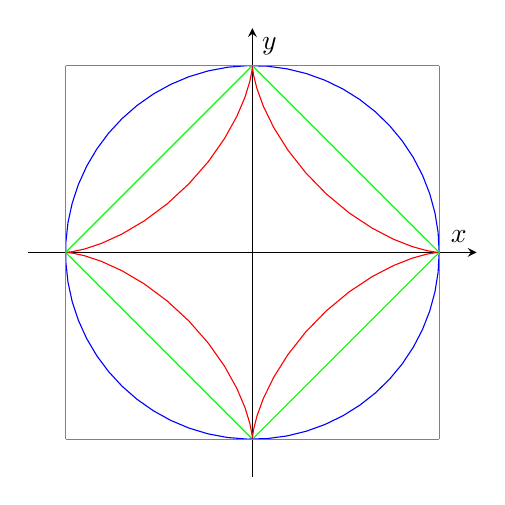
\begin{tikzpicture}
    \begin{axis}[
    axis equal image,
    axis lines = middle,
    enlargelimits,
    xtick=\empty,
    ytick=\empty,
    xlabel = {$x$},
    ylabel = {$y$},
    % legend pos = north east,
    % legend cell align = {left},
    % legend style = {draw=none}
  ]
    \addplot[domain=0:360, samples=60, red] ({cos(x)^(3)}, {sin(x)^(3)});
    % \addlegendentry{$p = 2/3$ (星形线)}
    \addplot[domain=0:360, samples=60, blue] ({cos(x)}, {sin(x)});
    % \addlegendentry{$p = 1$}
    \addplot[domain=0:360, samples=20, green] ({(cos(x)^(2))}, {sin(x)^(2)});
    \addplot[domain=0:360, samples=20, green] ({(-cos(x)^(2))}, {sin(x)^(2)});
    \addplot[domain=0:360, samples=20, green] ({(-cos(x)^(2))}, {-sin(x)^(2)});
    \addplot[domain=0:360, samples=20, green] ({(cos(x)^(2))}, {-sin(x)^(2)});
    % \addlegendentry{$p = 2$}
    \addplot[domain=-1:1, samples=2, cyan] (x,1);
    \addplot[domain=-1:1, samples=2, cyan] (x,-1);
    \addplot[domain=-1:1, samples=2, cyan] (1,x);
    \addplot[domain=-1:1, samples=2, cyan] (-1,x);
    % \addlegendentry{$p = 3$}
  \end{axis}
\end{tikzpicture}

\end{center}

注意其中的星形线$p = \frac{1}{3}$并不满足范数的定义,因为其不满足三角不等式

利用三角不等式的性质,我们能够说明在任何一个范数下,\textbf{单位圆都是凸的}

在1-范数空间内,$\pi = 4$

在$\infty$-范数空间内,$\pi = 4$

在2-范数空间内,$\pi \approx 3.1415\cdots$

如果作出一个$\pi$与$p$的关系图[先减后增],其中$2$-范数对应的$\pi$是最小值

等价范数:

如果存在$c_1,c_2$使得
\[c_1 \|\|_b \leq \|\|_a \leq c_2\|\|_b\]
则称范数$\|\|_a$和$\|\|_b$等价[这得益于齐次性]

\begin{definition}
  邻域
  \[U(x,r) \equiv \{y|d(x,y) < r\}\]
  去心邻域
  \[U(x,r) \equiv \{y|0 < d(x,y) < r\}\]
\end{definition}

\begin{definition}
  开集\\

  $E\subset X$,$\forall x \in E,\exists r$使得$U(x,r) \subset E$
\end{definition}
\begin{example}
  对于我们前面定义的平凡的距离空间,我们有任何集合都是一个开集
\end{example}

\begin{definition}
  收敛\\

  距离空间$(X,d)$中的点列$\{x_n\}$收敛到$x^\ast$,若$\forall \varepsilon > 0,\exists N > 0$使得$\forall n > N$都有$d(x_n,x^\ast) < \varepsilon$,我们记作
  \[\lim_{n \to +\infty} x_n = x^\ast\]
\end{definition}

\begin{definition}
  函数极限\\

  对于$f: X \to Y$,若$\forall \varepsilon >0$, $\exists \delta > 0$,使得当$d_1(x,x_0) < \delta$时,$d_2(f(x) - y_0) < \varepsilon$则称$x$趋近于$x_0$时$f(x)$收敛于$y_0$,记作
  \[\lim_{x \to x_0}f(x) = y_0\]
\end{definition}

\begin{definition}
  集合的聚点,孤立点\\

  集合$E$中的一个点称为聚点,若对$\forall r > 0$,$U_0(x,r) \bigcap E \neq \varnothing$

  集合$E$中的一个点称为孤立点,若对$\exists r > 0$,$U_0(x,r) \bigcap E = \varnothing$
\end{definition}

\begin{definition}
  集合的内点,外点,边界点\\

  内点:$\exists \delta >0$,$U(x,\delta) \subset E$
  
  所有内点组成的集合记为$\text{Int}(E)$

  外点: $\exists \delta > 0$,$U(x,\delta) \subset X \setminus E$

  所有外点的集合记为$\text{Ext}(E)$

  边界点: $\forall \delta >0$,使得$U(x,\delta) \bigcap E \neq \varnothing$并且$U(x,\delta) \bigcap X\setminus E \neq \varnothing$

  边界点的集合记为$\partial E$
\end{definition}

\begin{example}
  集合$\{\sqrt{2}m + n| m,n \in \NN\}$的边界点是全体实数
\end{example}

\begin{definition}
  闭集\\

  以下的两种定义是等价的:

  (1)开集的补集

  (2)$F \subset X$,任意的收敛点列$\{x_n\}$的极限都在集合中
\end{definition}

\begin{cproof}
  我们证明$1\to 2$,

  若不然,则$\lim_{n \to +\infty} x_n = x^\ast \in X\setminus F$,因此
  \[\forall \delta > 0,\exists x_n s.t. x_n \in U(x^\ast,\delta),x_n \notin X\setminus F\]
  这告诉我们$X\setminus F$不是开集,矛盾
\end{cproof}

\begin{definition}
  柯西列\\

  $\{x_n\} \subset X$,$\forall \varepsilon > 0$,$\exists N > 0$,使得$\forall n > N,p > 0$都有
  \[d(x_p,x_{n + p}) < \varepsilon\]
\end{definition}

\begin{theorem}
  收敛列是柯西列
\end{theorem}

\begin{cproof}
  $\forall \varepsilon > 0$,$\exists N$使得$\forall n > N$,$d(x_n,x^\ast)$,利用三角不等式,我们有
  \[d(x_n,x_{n + p} )\leq d(x_n,x^\ast ) + d(x^\ast,x_{n + p} ) < 2 \varepsilon\]
\end{cproof}

\subsection{空间的完备性}
\begin{definition}
  然而柯西列未必一定是收敛的,如果一个空间里所有柯西列都是收敛的,那么我们成这个空间为完备的\\
\end{definition}

注意这里的完备性是针对空间而言的,而之后的列紧,紧致等概念是针对集合的(虽然也可以对于全集)

\begin{definition}
  压缩映射\\

  映射$\varphi: X \to X$称为压缩映射,如果存在$0 < \alpha < 1$
  \[d(\varphi(x_1),\varphi(x_2)) \leq \alpha d(x_1,x_2)\]
\end{definition}

\begin{theorem}
  Banach不动点定理\\

  在完备距离空间$(X,d)$上的压缩映射有唯一不动点,也就是
  \[\exists! x^\ast \in X,~s.t. \varphi(x^\ast) = x^\ast\]
\end{theorem}

\begin{cproof}
  $\forall x_0 \in X$,$x_1 := \varphi(x_0)$,$\cdots$,$x_{n + 1} = \varphi(x_n)$,从而
  \[d(\varphi(x_{n + 1}), \varphi(x_n)) \leq \alpha d(\varphi(x_n),\varphi(x_{n - 1})) \leq \alpha^{n + 1} d(x_1,x_0)\]
  由于这个空间是完备的,从而任何一个柯西列都是收敛的,为此我们下面来构造一个柯西列
  \[
  \begin{aligned}  
    d(\varphi(x_{n + p}),\varphi(x_n)) &\leq d(\varphi(x_{n + p}),\varphi(x_{n + p - 1})) + \cdots + d(\varphi(x_{n + 1}),\varphi(x_n))\\
    &\leq(\alpha^{n + p} + \cdots + \alpha^{n + 1})\\
    &\leq \frac{\alpha^{n + 1}}{1 - \alpha} d(x_1,x_0) \\
  \end{aligned}  
  \]
  当$n\to +\infty$时,有上式$\to 0$,故前面我们构造的序列是柯西列,也是收敛序列

  \[d(\varphi(x^\ast),x^\ast) \leq d(\varphi(x^\ast),x_n) + d(x^\ast,x_n) \to 0\]
  这说明了$d(\varphi(x^\ast),x^\ast) = 0$ $\Rightarrow \varphi(x^\ast) = x^\ast$

  对于唯一性,我们假设还存在一个$y^\ast$,那么
  \[d(\varphi(x^\ast),\varphi(y^\ast)) = \alpha d(x^\ast,y^\ast) \]
  而又因为
  \[d(\varphi(x^\ast),\varphi(y^\ast)) =d(x^\ast,y^\ast) \]
  故$d(x^\ast,y^\ast) = 0$
\end{cproof}

\begin{theorem}
  $\RR^m(m > 1)$是一个赋范线性完备空间[Banach空间]
\end{theorem}
首先我们可以回忆$\RR$是完备的,即有对于任何柯西序列$\{x_n\}$满足,$\forall \varepsilon > 0, \exists N > 0,\forall n > N,p$使得
\[|x_n - x_{n + p} | < \varepsilon\]

都有$\{x_n\}$收敛,一种相对形象的理解方式是由于我们可以让$\varepsilon$每次缩小十倍,这样可以让极限一位位精确下去,从而实数域上的柯西序列一定收敛于某个实数

\begin{example}
  空间$\RR \setminus \QQ$不是完备的,因为$\frac{\sqrt{2}}{n} \notin \QQ$,但是极限$0 \in \QQ$
\end{example}

\begin{definition}
  $\RR$中的收敛点列\\

  对于$\{x_n\} \in \RR^m$,如果$\exists a \in \RR^m$,使得$\forall \varepsilon > 0,\exists N ,\forall n > N$都有
  \[\|x_n - a\| < \varepsilon\]
  使得
  \[\lim_{n \to +\infty} x_n = a\]
\end{definition}

\begin{theorem}
  $\{x_n\} \in \RR^m$ 收敛 $\Leftrightarrow$按坐标收敛
\end{theorem}
\begin{cproof}
  证明略
\end{cproof}

\begin{theorem}
  ``遗传定理'',例如
  
  (1)点列极限存在必唯一

  (2)线性运算和极限操作可交换

  (3)柯西收敛原理成立
\end{theorem}

\subsection{$\RR^m$空间中的函数}
\begin{definition}
  对于映射$f: \RR^m \to \RR$,集合$D \subset \RR^m$,$a$是$D$中的\textbf{聚点},如果$\exists A \in \RR$,对$U_0(a,  \eta) \cap d$上的$\forall $收敛序列$\{x_n\}$[注意这里必须包含所有收敛于$a$的点列],若
  \[\lim_{n \to +\infty}x_n = a\]
  都有
  \[\lim_{n \to +\infty }f(x_n) = A\]
  则称$f(x)$在$x$趋于$a$时沿$D$收敛到$A$
\end{definition}

\begin{definition}
  $\varepsilon-\delta$语言的定义

  $D \in \RR^m$,$a$是$D$中的\textbf{聚点},如果$\exists A \in \RR$,对$\forall \varepsilon > 0$,$\exists \delta > 0$,$\forall x \in D, \|x - a\| < \delta$,都有
  \[|f(x) - A| < \varepsilon\]
  则称
  \[{\lim_{x \to a}}_D f(x) = A\]
\end{definition}

利用遗传定理,我们可以证明这两种定义的等价性,我们省略

一个非常值得注意的是,极限是一个过程,要求了任意去心邻域含有其他点,否则无法产生这样一个趋近的过程
\begin{example}
  如何理解前面给出的``沿$D$收敛''

  \[f(x,y) = \begin{cases}
    \frac{xy}{x^2 + y^2}, &(x,y) \neq(0,0)\\
    0, &(x,y) = (0,0)\\
  \end{cases}\]

  当我们沿着$\frac{x}{y} = a$趋近于$(0,0)$时,我们发现
  \[f(x,y) = \frac{a}{1 + a^2}\]
  从而这个函数在$(0,0)$处的极限并不存在
\end{example}

\begin{theorem}
  函数乘积与复合函数的映射

  (1)若函数极限存在,则$\lim f \cdot g = \lim f g$

  (2)对于函数$f: \RR^m \to \RR$,$g: \RR \to \RR$,$g \circ f: \RR^m \to \RR$,若函数极限存在,且
  \[\lim_{x\to a}f(x) = b,\lim_{y \to b}g(y) = c\]

  则有
  \[\lim_{x\to a}g(f(x)) = c\]
\end{theorem}

\begin{definition}
  累次极限和重极限

  我们称$\lim_{x \to a}\lim_{y \to b} f(x,y)$形式的极限为累次极限[分多次取极限]

  称$\lim_{(x,y)\to(a,b)}f(x)$形式的极限为重极限\\

  当两个累次极限存在,重极限存在时,两个累次极限必然相等,因此如果两个累次极限存在但不相等时,重极限一定不存在

  累次极限只是重极限的一种特殊趋近方式,故重极限存在累次极限一定存在,反之不成立?对吗?

  不一定!先取极限的过程中,由于我们并没有连续性!先取的极限值和函数值并不一定相等!
\end{definition}
在不知道重极限是否存在的情况下慎用重极限换元法(求值的时候不存在问题)

极坐标变换要求极限过程对$\theta \in [0,2\pi)$是一致的

\begin{definition}
  多元函数的连续\\

  $a \in D \subset \RR^m$,$f(x)$在$U(a,\eta)\cap D$定义,若对$\forall U(a,\eta)\cap D$中的收敛点列$\{x_n\}$都有$\lim_{n \to +\infty}f(x_n) = f(a)$,则$f(x)$在$a$点处沿集合$D$连续
\end{definition}

\begin{definition}
  $\varepsilon-\delta$语言的定义\\

  $a \in D \subset \RR^m$,$f(x)$在$U(a,\eta)\cap D$定义,若对$\forall \varepsilon >0$,$\exists \delta > 0$,使得$\forall x \in U(a,\eta)\cap D, \|x - a\| < \delta$,都有
  \[|f(x) - f(a)| < \varepsilon\]
  则$f(x)$在$a$点处沿集合$D$连续,记作
  \[\lim_{x \to a}f(x) = f(a)\]
\end{definition}

\begin{definition}
  向量值函数的极限\\
  对于映射$f: \RR^m \to \RR^p$,集合$D \subset \RR^m$,$a$是$D$中的\textbf{聚点},如果$\exists A \in \RR^p$,对$\forall \varepsilon > 0$,$\exists \delta > 0$,$\forall x \in D, \|x - a\| < \delta$,都有
  \[\|f(x) - A\| < \varepsilon\]
  则称
  \[{\lim_{D \owns x \to a}} f(x) = A\]
\end{definition}
我们可以得出向量值函数极限存在/连续当且仅当各个分量函数极限存在/连续

\begin{theorem}
  开映射原理\\

  $f: \Omega \subset \RR^m \to \RR^p$,其中$\Omega$是一个开集,若$f \in C(\Omega) \Leftrightarrow \forall $开集$H \subset \RR^p$,其原像$f^{-1}(H)$也是开集
\end{theorem}

\begin{cproof}
  $\Rightarrow$:

  $\forall a \in f^{-1}(H)$,我们有$f(a) \in H$,而由于$H$是开集,故$\exists \eta \in \RR$,使得$U(f(a),\eta) \in H$,由于$f(x) \in C(\Omega)$,故对于$\eta$,$\exists \delta$使得$f(U(a,\delta)) \subset U(f(a),\eta) \subset H$
  故
  \[U(a,\delta) \subset f^{-1}(H)\]

  $\Leftarrow$:

  $\forall \varepsilon > 0,a \in \Omega$,定义$H := U(f(a),\varepsilon)$,由于$f^{-1}(H)$是一个开集,故$\exists \delta > 0$使得$U(a,\delta) \subset f^{-1}(H)$,故$f(U(a,\delta)) \subset H = U(f(a),\varepsilon)$,这个条件也就是函数连续性的定义
\end{cproof}

\subsection{有界闭集上连续函数的性质}

类比一元函数:闭区间连续函数有界,并且可以取到最大值和最小值

\begin{definition}
  集合的有界\\

  对$\RR^m$上的集合$E \subset \RR^m$,$\exists L \in \RR^+$使得$\forall x \in E$都有$\|x\| < L$ $\Leftrightarrow$ $\exists \tilde{L} \in \RR^+$使得$\forall x \in E$都有$|x^i| < L$ 
\end{definition}

\begin{theorem}
  B-W定理\\

  $\RR^m$中任意有界点列都有收敛子序列
\end{theorem}

\begin{cproof}
  这里的证明得益于此时空间维数的有限性,对从$1$到$m$的每个维度$k$,我们在原先$k - 1$个维度收敛的子序列的基础上取第$k$个维度也收敛的子列

  具体证明书写略
\end{cproof}

\begin{theorem}
  $E \subset \RR^m$是有界闭集,则$f\in C(E)$有界
\end{theorem}

\begin{cproof}
  反证法.若无界,则$\forall n$,$\exists x_n$使得$|f(x_n)| > n$,这样取$n = 1,2,\ldots$无限的取下去得到点列$\{x_n\}$,由于$E$有界,根据$B-W$定理,我们可以找到$\{x_n\}$的一个收敛子列,由于$E$是一个闭区间,则收敛子列收敛到的极限$x^\ast$也在$E$内,又由于$f$是一个连续函数
  \[\lim_{k\to +\infty} f(x_{n_k}) = f(x^\ast)\]
  这个极限是一个有限数,但这与$|f(x_{n_k})| > n_k$矛盾
\end{cproof}

\begin{theorem}
  $E\subset \RR^m$是有界闭集,$f\in C(E)$取到极值
\end{theorem}

\begin{cproof}
  $M = \sup_{x \in E} f(x)$,$\forall n$,$\exists x_n \in E$,使得
  \[M - \frac{1}{n} < f(x_n) < M\]
  并且对于有界闭集$E$,$\{x_n\}$存在一个收敛子列$\{x_{n_k}\}$当$k \to +\infty$时其收敛到$x^\ast \in E$.又由于$f\in C(E)$,我们有
  \[\lim_{k\to +\infty} f(x_{n_k}) = f(x^\ast)\]
  利用夹逼原理,我们知道
  \[M \leq \lim_{k\to +\infty} f(x_{n_k}) = f(x^\ast) \leq M\]
  极小值同理
\end{cproof}

\begin{theorem}
  $E \subset \RR^m$是有界闭集,$f\in C(E)$,则$f(x)$一致连续
\end{theorem}

\begin{cproof}
  反证法.假设$\exists \varepsilon_0$取$\delta = \frac{1}{n}$,$\exists x_n,x_n'$,$\|x_n - x_n'\| < \delta$但$|f(x_n) - f(x_n')| > \varepsilon_0$
  由$B-W$定理,按照前面的方式取序列,有$k\to +\infty$
  \[\|x_{n_k}' - x^\ast\| \leq \|x_{n_k}' - x_{n_k}\| + \|x_{n_k} - x^\ast\| \to 0\]
  利用$f$的连续性有,两个序列$f(x_{n_k})$和$f(x_{n_k}')$都收敛到相同的极限,这与我们前面的假设矛盾
\end{cproof}

\subsection{紧致性}
是什么东西给予了空间这样好的性质?

是因为其定义了一个比较好的距离度量

\begin{definition}
  列紧(sequential compactness)\\

  $E \subset X$是列紧的,若$\forall \{x_n\} \in E$,$\exists$收敛子列$\{x_{n_k}\}$,且$\lim_{k \to +\infty}x_{n_k} \in E$
\end{definition}

\begin{definition}
  覆盖\\

  $E \subset X$,若存在一族集合$\mathcal{V} = \{V_\alpha\}$,$V_\alpha \subset X$,$\forall x \in E$,$\exists V_\alpha$使得$x\in V_\alpha$,则我们称$\mathcal{V}$是$E$的一个覆盖

  若$V_\alpha$都是开集,则我们称$\mathcal{V}$是$E$的一个开覆盖
\end{definition}

\begin{definition}
  紧致\\

  $K \subset X$,若对$K$的任意开覆盖都有有限子覆盖
\end{definition}

\begin{lemma}
  有界闭集不一定是紧致集\\
\end{lemma}

\begin{example}
  对于有界闭集$X = \{\frac{1}{n}| n = 1,2,\ldots\}$,我们定义距离
  \[d = \begin{cases}
    0,x = y\\
    1,x\neq y\\
  \end{cases}\]
  我们构造一个开覆盖$\mathcal{V} = \{U(\frac{1}{n},\frac{1}{2}),n = 1,2,\ldots\}$,则不存在有限开覆盖
\end{example}

\begin{theorem}
  对于\textbf{任何一个距离空间},紧致$\Rightarrow$列紧$\Rightarrow$有界闭
\end{theorem}

\begin{cproof}
  紧致$\Rightarrow$列紧:

  反证法.假设不是列紧的,那么$\exists \{x_n\}$,其任意子列$\{x_{n_k}\}$都不收敛于$E$中的点,$\Rightarrow$ $\forall b \in E$,$\exists \eta_b$使得$U(b,\eta_b)$中只有$\{x_n\}$中的有限多元素.

  那么$\mathcal{V} = \{U(b,\eta_b),\forall b \in E\}$是$E$的开覆盖,利用紧致性,我们能从中选出一个有限子覆盖,而且每个集合中只有$\{x_n\}$中的有限个元素,也就是$E$中只有$\{x_n\}$中的有限个元素,矛盾.\\

  列紧$\Rightarrow$有界闭:

  (1)有界.反证:$\forall x_0 \in E$,$\forall n$,$\exists x_n$使得$d(x_0,x_n) > n$,由于$E$是列紧的,我们有$\exists \{x_{n_k} \to x^\ast \in E\}$.从而
  \[d(x_0,x_{n_k}) < d(x^\ast,x_0) + d(x^\ast,x_{n_k}) < d(x^\ast,x_0) + \varepsilon\]
  不等式最右边是一个有限数,这与前面的假设矛盾.\\

  (2)闭集.反证.$\exists \{y_n\} \in E$,$\{y_n\} \to b\notin E$,而利用列紧性,存在子列$\{y_{n_k}\} \to c \in E$,这就产生了矛盾[子列的极限必然和序列本身极限相等]
\end{cproof}

\begin{theorem}
  列紧$\Rightarrow$紧致
\end{theorem}

\begin{cproof}
  这个定理的证明省略
\end{cproof}

接下来我们回到$\RR^m$空间的情形考虑
\begin{theorem}
  Heine-Bord定理\\

  在$\RR^m$空间中,紧致$\Leftrightarrow$有界闭
\end{theorem}

\begin{cproof}
  $\Leftarrow$:根据有界的定义,存在正方体$I$使得$E \subset I$,我们首先证明$I$是紧致的\\

  \textbf{Step1:} $I$是紧致的.

  反证法:若不是,则$\exists$开覆盖$\mathcal{V}$,其没有有限子覆盖,我们参考一元情形的闭区间套原理,我们二分$I$的每个分量,得到$2^m$个有限子覆盖,则必然存在一个小方块$I_2$没有有限子覆盖,我们可以对$I_2$重复这样的过程,即有
  \[I = I_1 \supset I_2 \supset \cdots \supset I_n \supset \cdots\]
  于是$\forall n$,存在唯一的点$c \in I_n$[闭方块套原理,闭区间套原理的推广],由于$\mathcal{V}$是覆盖,那么一定存在$V^\ast$使得$c \in V^\ast$,由于$V^\ast$是一个开集,那么$\exists \delta$使得$U(c,\delta) \subset V^\ast$

  故$\exists N$,使得$\forall n > N$都有$I_n \subset U(c,\delta) \subset V^\ast$,这与$I_n$没有有限子覆盖矛盾\\

  \textbf{Step2:} 紧致集合的闭子集也是紧致的:利用$I$的紧致性证明$E$的紧致性

  对于有界闭集$E$的$\forall$ 开覆盖 $\mathcal{V}$,我们有$\tilde{\mathcal{V}} = \{\mathcal{V},\RR^m\setminus E\}$是$\RR^m$的开覆盖,[因为闭集的补集$\RR^m\setminus E$也是开集]
  
  显然$\RR^m$的开覆盖$\tilde{\mathcal{V}}$一定覆盖了$I$,又由于$I$是紧致集 $\Rightarrow$ 我们能从$\tilde{\mathcal{V}}$选出有限开覆盖 $\tilde{\mathcal{V}}^\ast = \{\mathcal{V}^\ast,\RR \setminus E\}$覆盖$I$,也就覆盖了$E$,由于$\RR^m \setminus E$对覆盖$E$没有任何帮助,故$\mathcal{V}^\ast$是$E$有限开覆盖\\

  重新反思我们的证明,事实上,再我们的Step2中并没有利用$\RR^m$的性质,事实上我们将$\RR^m$换成全空间$X$都是可以的,然而,在Step1中我们的闭区间块原理是依赖于$\RR^m$成立的:试想一下对于一个平凡的度量空间,每次将距离对半是不可操作的.
\end{cproof}

\begin{theorem}
  距离空间:紧致$\Rightarrow$完备[任意柯西列是收敛列]
\end{theorem}

\begin{cproof}
  对于柯西列$\{x_n\}$,$\forall \varepsilon > 0$,$\exists N > 0$,$\forall n > N,p > 0$,我们都有
  \[d(x_n - x_{n + p}) < \varepsilon\]

  紧致$\Rightarrow$列紧$\Rightarrow \exists$子列$\{x_{n_k}\} \to x^\ast$,利用三角不等式
  \[d(x_n,x^\ast) \leq d(x_n,x_{n_k}) + d(x_{n_k},x^\ast) < 2\varepsilon\]
  其中第一项小于$\varepsilon$,因为柯西收敛原理,第二项也小于$\varepsilon$,因为收敛子列的性质.
\end{cproof}

\begin{theorem}
  
  $(X,d)$是距离空间,$K \subset X$是紧致的,对于映射$f: K \to \RR$,$f \in C(K)$,则
  \begin{itemize}
    \item $f$有界
    \item $f$在$K$上取到极值
    \item $f$在$K$上一致连续
  \end{itemize}
  
\end{theorem}

\begin{cproof}
  (1)$f\in C(K) \Rightarrow \forall a \in K,\forall \varepsilon > 0,\exists \delta(a) > 0$,使得对$\forall x \in U(a,\delta(a)) \cap K$,有
  \[|f(x) - f(a)| < \varepsilon\]
  不妨取$\varepsilon = \varepsilon_0$,我们构造$\mathcal{V} = \{U(a,\delta(a)),a\in K\}$是$K$的开覆盖.\\

  因为$K$是紧致的,所以存在有限子覆盖$\tilde{\mathcal{V}} = \{U(a_i,\delta(a_i))\}_{i = 1,\ldots, N}$.

  任取$x \in K$,$\exists U(a_j,\delta(a_j))$使得$x \in U(a_j,\delta(a_j))$,
  \[|f(x)| \leq |f(a_j)| + \varepsilon \leq \max_{k = 1,\ldots,N} |f(a_k)| + \varepsilon\]
  最后使用了$f$的连续性以及我们子覆盖数量的有限性\\

  (2)不妨讨论极大值为例$M = \sup_{x\in K}f(x)$.利用上确界的定义,$\forall n$,$\exists x_n$使得
  \[M - \frac{1}{n} < f(x_n) \leq M\]

  紧致$\Rightarrow$列紧$\Rightarrow \exists$子列$\{x_{n_k}\} \to x^\ast \in K$,利用连续函数的性质
  \[\lim_{k \to +\infty}f(x_{n_k}) = f(\lim_{k \to +\infty} x_{n_k}) = f(x^\ast)\]

  反思我们在证明$\RR^m$中的有界闭集上取到极值的过程中使用的是B-W定理[而在一般的距离空间中,没有B-W定理,但是当集合为列紧集时,我们也有类似的性质]\\

  (3)$f\in C(K) \Rightarrow \forall a \in K,\forall \varepsilon > 0,\exists \delta(a) > 0$,使得对$\forall x \in U(a,\delta(a)) \cap K$,有
  \[|f(x) - f(a)| < \varepsilon\]

  我们取$\mathcal{V} = \{U(a,\frac{1}{2}\delta(a)),a\in K\}$作为$K$的开覆盖,利用$K$的紧致性,可知存在有限子覆盖$\tilde{\mathcal{V}} = \{U(a_i,\frac{1}{2}\delta(a_i))\}_{i = 1,\ldots,N}$.

  于是我们取$\forall x,x' \in K$,必然$\exists U(a_j,\frac{1}{2}\delta(a_j))$使得$x \in U(a_j,\frac{1}{2}\delta(a_j))$,于是我们取$\delta^\ast = \min_{j = 1,\ldots N} \frac{1}{2} \delta(a_j)$,于是$d(x,x') < \delta^\ast$可以推出
  \[d(a_j,x') \leq d(a_j,x) + d(x,x') < \frac{1}{2}\delta(a_j) + \delta^\ast < \delta(a_j)\]
  $\Rightarrow x' \in U(a_j,\delta(a_j))$,而根据我们前面所取得$\forall \varepsilon$,有$|f(x) - f(a_j)| < \varepsilon$.
  
  最后利用绝对值三角不等式,有
  \[|f(x) - f(x')| < |f(x) - f(a_j)| + |f(x') - f(a_j)| < 2\varepsilon\]
\end{cproof}

\subsection{连通性}

\begin{definition}
  路径\\

  如果对$E \subset \RR^m$,$x,y\in E$,若$\exists \gamma : [0,1] \to E$,$\gamma \in C[0,1]$且$\gamma(0) = x,\gamma(1) = y$,那么我们称$\gamma$是连接$x,y$的一条路径.
\end{definition}

\begin{definition}
  连通\\

  对于集合$E$,若$\forall x,y \in E$,都$\exists$ 路径$\gamma$连接$x,y$,则我们称$E$为路径连通的,简称连通.
\end{definition}

\begin{theorem}
  $E \subset \RR^m$是连通的,$f \in C(E)$,则$f$有介值性,即
  \[\forall A \in (\inf_{x \in E} f(x),\sup_{x\in E} f(x)),\exists x \in E ~s.t.~ f(x) = A\]
  这也可以表述为$\forall x,y \in E$,记$m = \min\{f(x),f(y)\},M = \max\{f(x),f(y)\}$,$\forall A \in [m,M]$,$\exists x \in E$使得$f(x) = A$
\end{theorem}

\begin{cproof}
  $E$连通$\Rightarrow \exists \gamma \in C[0,1]$使得$\gamma(0) = x,\gamma(1) = y$,那么$f \circ\gamma : [0,1] \to \RR$满足$(f \circ\gamma)(0) = f(x),(f \circ\gamma)(1) = f(y)$

  再利用一元连续函数的介值性我们知道$\forall A \in [m,M]$,$\exists c \in [0,1]$使得$(f \circ\gamma)(c) = A$,即在$\gamma(c)$上我们取到了这个介值
\end{cproof}

\begin{definition}
  区域\\

  开区域:$E$是开集且$E$连通

  闭区域:\textbf{开区域的闭包}
\end{definition}

\begin{example}
  在$\RR$中$(0,1)$是一个开区域;在$\RR^2$中$\{x\in(0,1),y = 0\}$不是一个开区域,因为其不是一个开集.
  
  在$\RR$中$[0,1]$是一个闭区域;在$\RR^2$中$\{x\in[0,1],y = 0\}$不是一个闭区域,因为$\{x\in(0,1),y = 0\}$不是一个开区域.
\end{example}

为什么我们要这么定义闭区域?

\begin{example}
  对于一个高维空间中的集合,两个部分之间如果只有一条一维的线相连,那么在很多时候并不``好用''
\end{example}

\begin{theorem}
  (开)闭区域上的连续函数有介值性[前面我们定义过程中只要求开区域是连通的,未要求闭区域一定连通]
\end{theorem}

\begin{cproof}
  若$x,y \notin \partial D$是显然的.\\

  我们考虑$x,y \in \partial D$的情况.若$m = M$,则情况显然,若$A = m$或$M$同样也是显然的.因此我们只考虑$A \in (m,M)$的情况.\\

  我们沿用前面的记号,由于$f(x)\in C(E)$,$\forall a \in D$,$\forall \varepsilon > 0$,$\exists \delta$,$\forall \tilde{x}\in U(a,\delta)$使得
  \[|f(\tilde{x}) - f(a)| < \varepsilon \]
  不妨取$\varepsilon = \frac{1}{2}(A - m)$,由于$D$是闭区域$\Rightarrow U(a,\delta) \cap \text{int} D \neq \varnothing$,也就$\exists x' \in U(a,\delta) \cap \text{int} D$,满足
  \[f(x') < f(a) + \varepsilon < A\]
  同理$x'' \in \text{int} D$使得
  \[f(x') > A\]
  再在$\text{int} D$内利用连通性证明介值性

\end{cproof}

\section{多元函数的导数}
\begin{definition}
  方向导数\\

  对于$\RR^m$中的向量$e$满足$\|e\| = 1$,我们定义$f(x)$在$e$方向上的方向导数为
  \[\frac{\partial f}{\partial e}(x) \equiv \lim_{t\to 0} \frac{f(x_0 + te) - f(x_0)}{t}\]
  
\end{definition}
对于这个定义,要注意的是我们这里定义的方向导数是利用直线而非射线定义的,也就是说本身强于由射线定义的方向导数,一种类比是,这种导数类似于一元情形下的导数,而由射线定义的方向导数则类似于一元情形下的单侧导数

\begin{definition}
  在$\RR^m$空间中,我们记第$i$个单位向量为$e_i$,那么我们将这些方向上的导数称为偏导数
  \[\frac{\partial f}{\partial x^i}(x) \equiv \frac{d}{dt}f(x + t e_i)|_{t = 0}\]
\end{definition}

根据这种基于直线的定义方式,我们知道各个方向导数存在则偏导数一定存在

\begin{definition}
  多元函数的梯度

  \[\nabla f = \parameter{\frac{\partial f}{\partial x^1},\frac{\partial f}{\partial x^2},\ldots,\frac{\partial f}{\partial x^m}}\]
\end{definition}

\begin{example}
  $f(x,y) = x^2 + y \sin x$

  \[\frac{\partial f}{\partial x} = 2x + y \cos x\]
  \[\frac{\partial f}{\partial y} = \sin x\]
  对于$e = (\cos \alpha,\sin \alpha)$,
  \[
    \begin{aligned}
      \frac{\partial f}{\partial e} &= \frac{d}{dt}f(x + t\cos \alpha,y + t\sin \alpha)|_{t = 0}\\
      &= \frac{d}{dt}|_{t = 0} \bracket{(x + t\cos \alpha)^2 + (y + t\sin \alpha) \sin (x + t\cos \alpha)}  \\
      &= \cos \alpha (2x + y \cos x) + \sin \alpha \sin x\\
      &= e\cdot \nabla f\\  
    \end{aligned}
    \]
\end{example}
是否对所有的函数都有这样好的性质呢?显然不是的
\begin{example}
  $f(x,y) = \begin{cases}
    0,x = 0 \text{或} y = 0\\
    x + y, otherwise\\
  \end{cases}$
  不难有
  \[\frac{\partial f}{\partial x}(0) = \frac{\partial f}{\partial y}(0) = 0\]
  然而我们取不沿坐标轴方向的$e = (\cos \alpha,\sin \alpha)$,则有
  \[\frac{\partial f}{\partial e} = \cos \alpha + \sin \alpha \neq e\cdot \nabla f\]
\end{example}

\begin{definition}
  可微\\

  对于函数$f:\RR^m\to \RR$和$x \in \RR^m$若在$x$的邻域内有
  \[f(x+h) = f(x) + L(x) h + o(h)\]
  其中$L(x)$为线性函数,$L(x) h = \sum_{i = 1}^{m} A^i(x) h^i$,$o(h) \equiv o(\|h\|)$则我们称$f(x)$在$x$可微
\end{definition}
  这里可微的内涵就是可以线性近似

  在我们进一步阐释之前,我们说明以下怎样的一个函数满足$o(h)$的情况:

\begin{example}
  对于$\RR^2$上的函数
  \[\varphi(h,k) = o(h) \Leftrightarrow \varphi(h,k) = \varepsilon(h) \sqrt{h^2 + k^2}~\text{或}~\varphi(h,k) = \alpha(h)h + \beta(h)k\]
  其中
  \[\lim_{(h,k)\to 0} \varepsilon,\alpha,\beta = 0\]
  这里上面一种情况也就是我们的定义本身,而上下两种情况的等价性需要我们的证明
\end{example}
\begin{cproof}
  第一种$\Rightarrow$:

  定义$\alpha \equiv \varepsilon\frac{h}{\|h\|}, \beta \equiv \varepsilon \frac{h}{\|h\|} \Rightarrow \varphi(h) = \alpha h + \beta k$\\

  第二种$\Leftarrow$:
  \[\frac{\varphi}{\|h\|} = \alpha\frac{h}{\|h\|} + \beta\frac{k}{\|h\|}\]
  我们在两式两侧取极限即可
\end{cproof}

在我们证明可微的过程中,我们通常利用$df$减去我们的线性部分也就是
\[f(x + h) - f(x) - \sum_{i = 1}^{m}A^i(x) h^i\]
来证明其是一个$o(h)$的量

\begin{theorem}
  可微$\rightarrow$连续
\end{theorem}

\begin{cproof}
  \[\lim_{h\to 0}\abs{f(x + h) - f(x)} = \lim_{h\to 0}\abs{L(x)h + o(h)} \leq \lim_{h \to 0} \parameter{\sum_{i = 1}^{m} |A^i(x)| |h^i| + |o(h^i)|} = 0\]
\end{cproof}

\begin{theorem}
  可微$\Rightarrow$可求方向导数
\end{theorem}

\begin{cproof}
  \[\frac{\partial f}{\partial e}(x) \equiv \frac{d}{dt}|_{t =  0} \parameter{\sum_{i = 1}^{m} A^i(x) t e^i + o(te^i)} = A^i(x)e^i\]
\end{cproof}

因此我们可以得出很多命题的强弱关系:

\begin{itemize}
  \item 可微$\Rightarrow$ 可方向导 $\Rightarrow$ 可偏导
  \item 可方向导$\nRightarrow$ 可微
  \item 可方向导$\nRightarrow$ 连续
\end{itemize}

\begin{theorem}
  对于 $\RR^2$ 空间上的函数$f(x) : \RR^2 \to \RR$和点$x_0 \in \RR^m$,若$\frac{\partial}{\partial x}f(x,y),\frac{\partial}{\partial y}f(x,y)$存在且在$x_0$处连续,则$f(x)$在$x_0$处可微
\end{theorem}

\begin{cproof}
  \[\begin{aligned}
    f(x_0 + h,y_0 + k) - f(x_0,y_0) &= f(x_0 + h,y_0 + k) - f(x_0 + h,y_0) + f(x_0 + h,y_0) - f(x_0,y_0)\\
    &= \frac{\partial f}{\partial y}(x_0+h,y_0)k + o(k) +\frac{\partial f}{\partial x}(x_0,y_0)h + o(h)\\
    &= \parameter{\frac{\partial f}{\partial y}(x_0,y_0) + o(h
    )}k + o(k) +\frac{\partial f}{\partial x}(x_0,y_0)h + o(h)\\    
    &=\parameter{\frac{\partial f}{\partial x}(x_0,y_0)h + \frac{\partial f}{\partial y}(x_0,y_0)k } + o(h)\\ 
  \end{aligned}\]
\end{cproof}

\begin{theorem}
  $f(x,y)$的两个偏导数$\frac{\partial f}{\partial x}$,$\frac{\partial f}{\partial y}$在$(x_0,y_0)$的某一邻域内存在且有界,则$f(x,y)$在$(x_0,y_0)$处\textbf{连续}(不是可微!)
\end{theorem}

\begin{cproof}
  我们记$\Delta x = h, \Delta y = k$
  \[\begin{aligned}
    \Delta f = f(x_0 + h,y_0 + k) - f(x_0,y_0) &= f(x_0 + h,y_0 + k) - f(x_0,y_0 + k) + f(x_0,y_0 + k) - f(x_0,y_0) \\
    &= \frac{\partial f}{\partial x}(x_0 + \theta_1h,y_0 + k)h + \frac{\partial f}{\partial y}(x_0,y_0 + \theta_2 k)k\\
  \end{aligned}\]
  利用一元函数的微分中值定理[这里是拉格朗日中值定理]

\end{cproof}

\begin{definition}
  $\Omega \subset \RR^m$中的区域,若$f$各偏导数存在且连续,那么则称$f$在$\Omega$上是连续可微的
\end{definition}

偏导数的几何意义在$f:\RR^2\to\RR$的情况下最为显著,我们每个偏导数都可以对应于一个曲面的切向量,即
\[\ve{u}_1 = (1,0,\frac{\partial f}{\partial x}),\ve{u}_2 = (0,1,\frac{\partial f}{\partial x})\]
我们可以利用叉乘的方法得到法向量
\[\ve{n} = (-\frac{\partial f}{\partial x},-\frac{\partial f}{\partial y},1)\]
利用法向量可以得到切平面


\begin{theorem}
  复合函数的导函数\\

  对于可微函数$f(x):\RR^m \to \RR ,\varphi(t): \RR \to \RR^m$,$f(\varphi(t))$的导数满足
  \[f'(\varphi(t)) = \sum_{i = 1}^{m} \frac{\partial f}{\partial x^i}\frac{d\varphi^i}{d t}  \]
\end{theorem}

\begin{cproof}
  我们记$x = \varphi(t)$,从而有$\Delta x = \varphi(t + \Delta t) - \varphi(t)$,那么利用一小段差
  \[\begin{aligned}
    f(\varphi(t + \Delta t)) - f(\varphi(t)) &= f(x + \Delta x) - f(x)\\
    &= \sum_{i = 1}^{m} \frac{\partial f}{\partial x^i} \Delta x^i + o(\Delta x)\\
    &= \sum_{i = 1}^m \frac{\partial f}{\partial x^i}\parameter{\frac{d \varphi^i}{dt}\Delta t + o(\Delta t)} + o(\Delta x)\\
    &= \sum_{i = 1}^m \frac{\partial f}{\partial x^i}\frac{d \varphi^i}{dt}\Delta t + o(\Delta t)\\
  \end{aligned}\]
\end{cproof}

当我们将$\varphi(t)$的定义域由$\RR$改为$\RR^n$时,我们可以进行类似的证明

\begin{theorem}
  复合函数的导函数\\

  对于可微函数$f(x):\RR^m \to \RR ,\varphi(t): \RR^n \to \RR^m$,$f(\varphi(t))$的导数满足
  \[f'(\varphi(t)) = \sum_{i = 1}^{m}\sum_{j = 1}^{n} \frac{\partial f}{\partial x^i}\frac{\partial \varphi^i}{\partial t^j}  \]
\end{theorem}
我们可以将这样的式子写成矩阵的形式
\[\begin{pmatrix}
  \dfrac{\partial y}{\partial t^1}&\dfrac{\partial y}{\partial t^2}&\cdots&\dfrac{\partial y}{\partial t^n}
\end{pmatrix} = \begin{pmatrix}
  \dfrac{\partial y}{\partial x^1}&\dfrac{\partial y}{\partial x^2}&\cdots&\dfrac{\partial y}{\partial x^m}
\end{pmatrix} \begin{pmatrix}
  \dfrac{\partial x^1}{\partial t^1}&\cdots&\dfrac{\partial x^1}{\partial t^n}\\
  \vdots&\ddots&\vdots\\
  \dfrac{\partial x^m}{\partial t^1}&\cdots&\dfrac{\partial x^m}{\partial t^n}\\
\end{pmatrix}\]

同理我们可以继续推广:

对于可微函数$f(x):\RR^m \to \RR^p ,\varphi(t): \RR^n \to \RR^m$,$f(\varphi(t))$的导数可以写成矩阵形式

\[\begin{pmatrix}
  \dfrac{\partial y^1}{\partial t^1}&\dfrac{\partial y^1}{\partial t^2}&\cdots&\dfrac{\partial y^1}{\partial t^n}\\
  \vdots&\vdots&\ddots&\vdots\\
  \dfrac{\partial y^p}{\partial t^1}&\dfrac{\partial y^p}{\partial t^2}&\cdots&\dfrac{\partial y^p}{\partial t^n}\\
\end{pmatrix}_{p \times n} = \begin{pmatrix}
  \dfrac{\partial y^1}{\partial x^1}&\dfrac{\partial y^1}{\partial x^2}&\cdots&\dfrac{\partial y^1}{\partial x^m}\\
  \vdots&\vdots&\ddots&\vdots\\
  \dfrac{\partial y^p}{\partial x^1}&\dfrac{\partial y^p}{\partial x^2}&\cdots&\dfrac{\partial y^p}{\partial x^m}\\
\end{pmatrix}_{p \times m} \begin{pmatrix}
  \dfrac{\partial x^1}{\partial t^1}&\cdots&\dfrac{\partial x^1}{\partial t^n}\\
  \vdots&\ddots&\vdots\\
  \dfrac{\partial x^m}{\partial t^1}&\cdots&\dfrac{\partial x^m}{\partial t^n}\\
\end{pmatrix}_{m \times n}\]

\subsubsection{复合函数的微分}
首先我们来看多元函数微分的本质

由于$f$可微:
\[f(x + \Delta x) - f(x) = \mathcal{L}_f \Delta x+ o(\Delta x)\]
本质上我们要构建一个从定义域某点处$x$的切空间$T\RR^m(x)$到值域某处$y$处切空间$T\RR(y)$的映射$df(x)$,则有

为什么我们要定义一个切空间?因为$dx$和$dy$分别是以$x$和$y$为原点的向量
\[df(x)(dx) = \mathcal{L}_f(x)\, dx = \frac{\partial f}{\partial x^i}(x) \, dx^i\]

\begin{theorem}
  微分的性质\\

  对于可微函数$f,g : \RR^m \to \RR$,$\lambda,\mu \in \RR$,我们构造$\lambda f + \mu g: \RR^m \to \RR$

  我们有
  \[\lambda df + \mu dg = d(\lambda f + \mu g)\]

  同理我们也可以证明: 
  \[d(fg) = g \, df + f \, dg\]
\end{theorem}

\begin{cproof}
  \[
    \begin{aligned}
      (\lambda f + \mu g)(x + \Delta x) - (\lambda f + \mu g)(x)&= \lambda(f(x+\Delta x) - f(x)) + \mu (g(x + \Delta x) - g(x))\\
      &= \lambda(\mathcal{L}_f(x) \Delta x + o(\Delta x)) + \mu (\mathcal{L}_g(x) + o(\Delta x))\\
      &= (\lambda\mathcal{L}_f(x) + \mu \mathcal{L}_g(x))\Delta x + o(\Delta x)\\
      &= \mathcal{L}_{\lambda f + \mu g}(x) \Delta x + o(\Delta x)\\
    \end{aligned} \]
\end{cproof}

\begin{theorem}
  复合函数的微分\\

考虑复合映射$\RR^n \to \RR^m \to \RR^p$,$f\circ \varphi$,我们的微分实质上在切空间上进行了如下的映射$T\RR^n(t) \to T\RR^m(x) \to T\RR^p(y)$

那么我们可以将每个切空间中的小向量表示为
\[dx = \mathcal{L}_{\varphi(t)} \, dt\]
\[dy = \mathcal{L}_{f(x)} \, dx = \mathcal{L}_{f(x)} \mathcal{L}_{\varphi(t)} \, dt \]

\end{theorem}
写成矩阵的形式也就是
\[\begin{pmatrix}
  dy^1\\
  dy^2\\
  \vdots\\
  dy^p\\
\end{pmatrix} = \begin{pmatrix}
  \dfrac{\partial y^1}{\partial x^1}&\dfrac{\partial y^1}{\partial x^2}&\cdots&\dfrac{\partial y^1}{\partial x^m}\\
  \vdots&\vdots&\ddots&\vdots\\
  \dfrac{\partial y^p}{\partial x^1}&\dfrac{\partial y^p}{\partial x^2}&\cdots&\dfrac{\partial y^p}{\partial x^m}\\
\end{pmatrix}_{p \times m} \begin{pmatrix}
  \dfrac{\partial x^1}{\partial t^1}&\cdots&\dfrac{\partial x^1}{\partial t^n}\\
  \vdots&\ddots&\vdots\\
  \dfrac{\partial x^m}{\partial t^1}&\cdots&\dfrac{\partial x^m}{\partial t^n}\\
\end{pmatrix}_{m \times n} \begin{pmatrix}
  dt^1\\
  dt^2\\
  \vdots\\
  dt^n\\
\end{pmatrix}\]

\begin{theorem}
  一阶微分的不变性\\

  当$x$是自变量时,我们有微分式
  \[d y^i = \frac{\partial y^i}{\partial x^j} d x^j\]

  当$x$是关于$t$的函数时,我们有微分式
  \[d y^i = \frac{\partial y^i}{\partial t^k} d t^k = \frac{\partial y^i}{\partial x^j}\frac{\partial x^j}{\partial t^k} d t^k = \frac{\partial y^i}{\partial x^j} dx^j\]
  无论$x$是否是自变量,我们都有同样的形式[注:这里我们使用了哑标求和]
\end{theorem}

\begin{example}
  对于
  \[\begin{cases}
    x = r \cos \theta\\
    y = r \sin \theta\\
  \end{cases}\]
  我们有偏导数的关系
  \[\begin{pmatrix}
    \frac{\partial f}{\partial r}&\frac{\partial f}{\partial \theta}\\
  \end{pmatrix} = \begin{pmatrix}
    f_x&f_y\\
  \end{pmatrix} \begin{pmatrix}
    \cos \theta & - r\sin \theta\\
    \sin \theta & r \cos \theta\\
  \end{pmatrix}\]
  写成微分的关系有
  \[\begin{pmatrix}
    dx\\
    dy\\
  \end{pmatrix} = \begin{pmatrix}
    \cos \theta & - r\sin \theta\\
    \sin \theta & r \cos \theta\\
  \end{pmatrix} \begin{pmatrix}
    dr \\
    d\theta\\
  \end{pmatrix}\]
  事实上我们利用$x,y$表示$r,\theta$可以得到
  \[\begin{pmatrix}
    dr \\
    d\theta\\
  \end{pmatrix}= \begin{pmatrix}
    \cos \theta & \sin \theta\\
    -\frac{1}{r}\sin \theta & \frac{1}{r} \cos \theta\\
  \end{pmatrix} \begin{pmatrix}
    dx\\
    dy\\
  \end{pmatrix} \]  
  以上两个Jacobi行列式互为逆,我们利用这个也可以证明一阶微分的不变性,在这里即是
  \[f_r \, dr + f_\theta\, d\theta = df = f_x \, dx + f_y \, dy\]
\end{example}

\begin{example}
  对于$\varphi$: 
  \[\begin{cases}
    p = x\\
    q = x + y\\
  \end{cases}\]
  和任意一个$f: \RR^2 \to \RR$,注意
  \[\frac{\partial f }{\partial p} = \frac{\partial f }{\partial x} \frac{\partial x}{\partial p} + \frac{\partial f }{\partial y} \frac{\partial y}{\partial p} = \frac{\partial f }{\partial x} - \frac{\partial f }{\partial y}\]
  但是我们知道$p = x$,那么是不是说
  \[\frac{\partial f }{\partial p} = \frac{\partial f }{\partial x} = \frac{\partial f }{\partial x} - \frac{\partial f }{\partial y}\]
  呢?

  并不是这样,要注意到本质上两套变量本质上提供了两组坐标,而求偏导的过程是在保持其余坐标变量不变的情况下对某个变量求导,然而,上面两个式子中保持不变的量是不同的,也就是事实上有
  \[\frac{\partial f }{\partial p}|_{(x,x+y)} = \frac{\partial f }{\partial x} = \frac{\partial f }{\partial x}|_{(x,y)} - \frac{\partial f }{\partial y}|_{(x,y)}\]
\end{example}
\subsection{高阶导数}

\begin{definition}
  定义高阶偏导数为
  \[\partial_x(\partial x f(x,y)) := \partial_{xx}f(x,y) := \frac{\partial f}{\partial x \partial x}(x,y) \]
  \[\partial_y(\partial x f(x,y)) := \partial_{xy}f(x,y) := \frac{\partial f}{\partial y \partial x}(x,y) \]
  \[\partial_x(\partial y f(x,y)) := \partial_{yx}f(x,y) := \frac{\partial f}{\partial x \partial y}(x,y) \]
  \[\partial_y(\partial y f(x,y)) := \partial_{yy}f(x,y) := \frac{\partial f}{\partial y \partial y}(x,y) \]
  注意右侧两种写法中的$x,y$的先后顺序.

  那么我们会考虑一件事,例如上面的第二种和第三种偏导数,它们的值相等吗?
\end{definition}

\begin{theorem}
  若$f_{xy}(x,y)$和$f_{yx}(x,y)$在$x_0$附近存在且在$x_0$连续,则$f_{xy}(x_0) = f_{yx}(x_0)$
\end{theorem}

\begin{cproof}
  \[f_x(x_0,y_0) = \lim_{h\to 0}\frac{f(x_0 + h,y_0) - f(x_0,y_0)}{h}\]
  \[f_{xy}(x_0,y_0) = \lim_{k\to 0}\frac{f_x(x_0,y_0 + k) - f_x(x_0,y_0)}{k}\]

  我们记目标函数为[这个式子可以通过将上面两个式子去除极限号然后移项来不严谨的得到]
  \[f(x_0 +h,y_0 + k) - f(x_0,y_0 + k) - f(x_0 + h,y_0) + f(x_0,y_0)\]
  我们记$\varphi(x) = f(x,y_0 + k) - f(x,y_0)$,从而我们可以把目标式子写作$\varphi(x_0 + h) - \varphi(x_0)$,由于
  利用微分中值定理,转化上式为
  \[
  \begin{aligned}
    &= \varphi_x(x_0 + \theta_1 h)h\\
    &= h\bracket{f_x(x_0 + \theta_1 h,y_0 + k) - f_x(x_0 + \theta_1 h,y_0)}\\
    &= hk f_{xy}(x_0 + \theta_1 h, y_0 + \theta_2 k)\\
  \end{aligned}  
  \]

  同理,上式也可以写作
  \[hk f_{yx}(x_0 + \theta_3 h,y_0 + \theta_4 k)\]
  由于$f_{xy}$和$f_{yx}$在$x_0$处连续,因此我们可以得到$\theta_1 h,\theta_2 k,\theta_3 h,\theta_4 k$都$\to 0$,从而也就证明了
  \[f_{xy}(x_0,y_0) = f_{yx}(x_0,y_0)\]
\end{cproof}
\begin{theorem}
  $f:\RR^m \to \RR$,$f\in C^{(k)}(\Omega)$,$\Omega \subset \RR^m$是开集,则
  \[\partial_{x^{i_1} \cdots x^{i_r}}f(x) = \partial_{x^{\tilde{i}_1} \cdots x^{\tilde{i}_r}}f(x)\]
  其中$\tilde{i}_1,\ldots,\tilde{i}_r$是对$i_1,\ldots,i_r$的重排,且有$r \leq k$
\end{theorem}

\begin{cproof}
  利用归纳法,其中$r = 2$的情况我们已经证明成立,假设$n = r$的情况成立,下面证明对于$n = r + 1 \leq k$的情况也成立
  \[
  \begin{aligned} 
    \partial_{x^{i_1} x^{i_2} \cdots x^{i_{k + 1}}} f &= \partial_{x^{i_1}}\parameter{\partial_{ x^{i_2} \cdots x^{i_{k + 1}}} f}\\
    &=\partial_{x^{i_1} } \partial_{x^{i_2} }\parameter{\partial_{ x^{i_3} \cdots x^{i_{k + 1}}} f}\\
    &=\partial_{x^{i_2} } \partial_{x^{i_1} }\parameter{\partial_{ x^{i_3} \cdots x^{i_{k + 1}}} f}\\
    &= \partial_{x^{i_2} x^{i_1} \cdots x^{i_{k + 1}}} f
  \end{aligned}  
   \]
   从而我们实现了其中两个偏导的位置交换,同理可以实现任意两个位置的兑换,从而实现所有的排列
\end{cproof}

\begin{definition}
  梯度的散度

  \[\nabla \cdot (\nabla f) = \nabla^2 f = \Delta f\]

  其中$\Delta$是拉普拉斯算子
\end{definition}

\begin{theorem}
  链式法则与高阶偏导数\\

  \[\frac{\partial y}{\partial t^i} = 
  \sum_{j = 1}^{m} \frac{\partial y}{\partial x^j}\frac{\partial x^j}{\partial t^i}\]

  那么二阶偏导数就有
  \[
  \begin{aligned}  
    \frac{\partial^2 y}{\partial t^k \partial t^i} = \frac{\partial}{\partial t^k}\parameter{\frac{\partial y}{\partial t^i}} &= \sum_{j = 1}^{m}  \frac{\partial}{\partial t^k}\parameter{\frac{\partial y}{\partial x^j}}\frac{\partial x^j}{\partial t^i} +\sum_{j = 1}^{m} \frac{\partial y}{\partial x^j} \frac{\partial}{\partial t^k}\parameter{\frac{\partial x^j}{\partial t^i}} \\
    &= \sum_{l = 1}^{m}\sum_{j = 1}^{m} \frac{\partial y^2}{\partial x^l \partial x^j} \frac{\partial x^l}{\partial t^i}\frac{\partial x^j}{\partial t^i} + \sum_{j = 1}^{m} \frac{\partial y}{\partial x^j} \frac{\partial^2 x^j}{\partial t^i \partial t^i}\\
  \end{aligned}  
  \]

  我们将这个结果写成矩阵的形式,对于一阶的情形,也就有
  \[\begin{pmatrix}
    \dfrac{\partial y}{\partial t^1}&\dfrac{\partial y}{\partial t^2}&\cdots&\dfrac{\partial y}{\partial t^n}
  \end{pmatrix} = \begin{pmatrix}
    \dfrac{\partial y}{\partial x^1}&\dfrac{\partial y}{\partial x^2}&\cdots&\dfrac{\partial y}{\partial x^m}
  \end{pmatrix} \begin{pmatrix}
    \dfrac{\partial x^1}{\partial t^1}&\cdots&\dfrac{\partial x^1}{\partial t^n}\\
    \vdots&\ddots&\vdots\\
    \dfrac{\partial x^m}{\partial t^1}&\cdots&\dfrac{\partial x^m}{\partial t^n}\\
  \end{pmatrix}\]

  对于二阶导数的情形,也就有
  \[
  \begin{aligned}
  \frac{\partial^2 y}{\partial t^k \partial t^i} = \begin{pmatrix}
    \dfrac{\partial x^1}{\partial t^k}&\cdots&\dfrac{\partial x^m}{\partial t^k}\\
  \end{pmatrix}&
  \begin{pmatrix}
    \frac{\partial^2 y}{\partial x^1 \partial x^1}&\cdots&\frac{\partial^2 y}{\partial x^1 \partial x^m}\\
    \vdots&\ddots&\vdots\\
    \frac{\partial^2 y}{\partial x^m \partial x^1}&\cdots&\frac{\partial^2 y}{\partial x^m \partial x^m}\\
  \end{pmatrix}
  \begin{pmatrix}
    \dfrac{\partial x^1}{\partial t^i}\\
    \vdots\\
    \dfrac{\partial x^m}{\partial t^i}\\
  \end{pmatrix}\\ &+ 
  \begin{pmatrix}
    \dfrac{\partial y}{\partial x^1}&\dfrac{\partial y}{\partial x^2}&\cdots&\dfrac{\partial y}{\partial x^m}
  \end{pmatrix}
  \begin{pmatrix}
    \frac{\partial^2 x^1}{\partial t^k \partial t^i}\\
    \vdots\\
    \frac{\partial^2 x^m}{\partial t^k \partial t^i}\\
  \end{pmatrix}
  \end{aligned}  
  \]
\end{theorem}

\begin{theorem}
  高阶微分的形式\\

  我们用高阶导数中的记号,我们就有
  \[\begin{aligned}
    d^2 y &= \sum_{i,j} \frac{\partial^2 y}{\partial x^i \partial x^j} d x^i d x^j\\
    &= \sum_{i,j,k,l} \frac{\partial^2 y}{\partial x^i \partial x^j} \frac{\partial x^i}{\partial t^k} \frac{\partial x^j}{\partial t^l} d t^k d t^l + \sum_{i,k,l} \frac{\partial y}{\partial x^j}\frac{\partial^2 x^j}{\partial t^k \partial t^l} d t^k d t^l\\
  \end{aligned}\]
\end{theorem}

\subsection{多元函数的泰勒公式}
\subsubsection{多元函数的泰勒公式}
回顾一元的泰勒公式
对于$f:\RR \to \RR$,例如定义$f(x) \in C^{(n + 1)}[x,x + \Delta x]$,那么我们可以进行如下的近似
\[f(x + \Delta x) = f(x) + f'(x) \Delta x+ \cdots = f(x) + \sum_{k = 1}^{n}f^{(k)}(x) \Delta x^k + R_{n + 1}\]

其中$R_{n + 1}$是余项,常见的余项有
\begin{itemize}
  \item Peano余项 $R_{n + 1} = o(\Delta x^n)$
  \item Lagrange余项 $R_{n + 1} = \frac{1}{(n + 1)!}f^{(n + 1)}(x + \theta \Delta x) \Delta x^{n + 1}, \theta \in (0,1)$
  \item 积分余项 $R_{n + 1} = \frac{1}{n!} \int_{0}^{1}(1 - t)^{n} f^{(n + 1)}(x + t\Delta x)\, dt$
  \item Cauchy余项 $R_{n + 1} = \frac{1}{n!} (1 - \theta)^n f^{(n + 1)}(x + \theta \Delta x) \Delta x^{n + 1}, \theta \in (0,1)$
\end{itemize}

我们怎样获得多元函数的泰勒公式呢?因为我们可以有多个方向.

对于一个多元函数$f: \RR^m \to \RR$我们的Idea是利用类似于方向导数一样的方法一样给定一个方向$\Delta x $,于是我们就可以定义一个$\varphi: \RR \to \RR$
\[\varphi(t) \equiv f(x + t \Delta x)\]

那么我们可以在$t = 0$处利用一元函数的泰勒公式,也就有
\[\varphi(t) = \varphi(0) + \sum_{k = 1}^{n} \frac{1}{k!}\varphi^{(k)}(0)t^k + R_{n + 1}\]

而我们知道
\[\varphi^{(1)}(t) = \Delta x \cdot \nabla f(x + t \Delta x)\]

推而广之也就有
\[\varphi^{(k)}(t) = (\Delta x \cdot \nabla)^k f(x + t \Delta x)\]

注意这里的$\Delta x \cdot \nabla$其实就是
\[\sum \Delta x^i \partial_{x^i}\]

那么我们怎样表示余项呢?不妨考虑积分余项

\[
\begin{aligned}
  R_{n + 1} &= \frac{1}{n!} \int_{0}^{1}(1 - t)^{n} \varphi^{(n + 1)}(x + t\Delta x)\, dt\\
  &= \frac{1}{n !} \int_{0}^{1}(1 - t)^n (\Delta x \cdot \nabla)^{n + 1} f(x + t\Delta x)\, dt\\
\end{aligned}  
\]

由于我们是在$t = 0$处展开的
\[f(x + \Delta x) = \sum_{k = 1}^{n} \frac{1}{k !}(\Delta x \cdot \nabla)^k f(x) + R_{n + 1}\]

我们可以利用中值定理将积分余项转化为柯西余项
\[\frac{1}{n !} (1 - \theta)^n (\Delta x \cdot \nabla)^{n + 1}f(x + \theta\Delta x),\theta \in (0,1) \]

拉格朗日余项同理可以导出

\[\frac{1}{(n + 1)!} (\Delta x \cdot \nabla)^{n + 1} f(x + \theta \Delta x),\theta \in (0,1)\]

主要是下面的Peano余项

\[\sum A^j \prod_{i = 1}^{m}(\Delta x^i)^{p_i^j}  (\sum_{i = 1}^{m}p_i^j = n + 1)\]

注意这里的$A^j$代表了我们的各$(n + 1)$阶偏导数,而最外层的求和代表遍历所有的$p_i$的分配方式.从而我们可以知道其是满足
\[o(\Delta x^n)\]
\subsubsection{有限增量公式}
当我们取$n = 0$时,我们就得到了多元情形的有限增量公式

\begin{theorem}
  \[f(x + \Delta x) = f(x) + \int_{0}^{1} \Delta x \cdot \nabla f(x + t\Delta x)\, dt\]

  或者写作拉格朗日余项
  \[f(x + \Delta x) = f(x) + \Delta x \cdot\nabla f(x + \theta\Delta x)\]
\end{theorem}

\begin{theorem}
  对于$f: \RR^m \to \RR$,在开区域$D \subset \RR^m$上可微,若$\nabla \cdot f = 0$,则$f(x) = const$
\end{theorem}
这个定理我们不能简单的使用有限增量公式来证明,因为我们取的$x + \theta \Delta x$未必在我们的区域内,因此我们需要利用开区域的连通性来给出证明
\begin{cproof}
  对于$D$上的任意两点$x,y$,我们可以找到连续的函数$\gamma$满足
  \[\gamma t = \begin{cases}
    x ,t = 0\\
    y, t = 1\\
  \end{cases}\] 

  要注意这条路径$\gamma$一定是连续的,但不一定是可微的!,因此不能简单的利用链式法则来处理\\

  (1)若$D = U(a,\delta)$开球,那么我们可以直接利用有限增量公式来证明,
  \[f(x + \Delta x) = f(x) + \Delta x \cdot \nabla f(x + \theta \Delta x) ,\theta \in (0,1)\]

  其中$x + \theta \Delta x$一定在我们的开球内,因此我们也就证明了我们的结论\\

  对于更广泛的情形,即

  (2)$D$是一般开区域,那么按照前面分析中的方法任取$x,y \in D$,构造我们的路径$\gamma$满足$\gamma(0) = x, \gamma(1) = y$

  我们运用反证法,假设我们的$f(x) \neq f(y)$,那么我们一定存在
  \[\sigma = \sup\{t|f(\gamma(t)) = f(x)\}\]

  又因为$D$是开的,那么在$\sigma$周围一定存在邻域$U(\sigma,\eta) \subset D$,那么利用前面我们证明的开球的情形,$\forall z \in U(\sigma,\eta)$,我们都有$f(z) = f(\gamma(\sigma))$,然而由于$\gamma$是连续的,因此一定存在$\tau > \sigma$使得$\gamma(\tau) \in U(\sigma,\eta)$,并且同样有$f(\gamma(\tau)) = f(x)$.

  这与我们之前取的上确界矛盾.故我们的$f(x) = f(y)$必然成立.又因为我们这里选的$x,y$是任取的,从而我们证明了$f$在$D$上是一个常值函数
\end{cproof}

\subsection{隐函数定理}

对于$F(x,y)$定义在$D \times E(x \in D,y \in E)$,若$\forall x, \exists ! y$使得$F(x,y) = 0$,称$F(x,y) = 0$唯一确定了一个从$D$到$E$的函数,那么在什么条件下有这样的性质成立呢?

如果$F(x,y)$是可微的,那么我们可以有
\[d F(x,y) = F_x \,dx + F_y \, dy\]

从而有
\[F(x + \Delta x, y + \Delta y) - F(x,y) = F_x \,dx + F_y \, dy + o(\Delta x)\]

那么我们可以形式的写出$\Delta y \approx - \frac{F_x}{F_y} \Delta x$,那么我们应该在这个邻域内有$F_y \neq 0$

\begin{theorem}
  隐函数定理\\

  对于$F:\Omega \to \RR$,$\Omega \subset \RR^2$,$(x_0,y_0) \in \Omega$,若有以下条件成立:
  \[(1)F\in C^{(1)}(\Omega),(2)F(x_0,y_0) = 0,(3)F_y(x_0,y_0) \neq 0\]

  则$\exists \alpha,\beta > 0$,$D = \{x\in \RR| |x - x_0| < \alpha\},E \{y\in \RR||y - y_0 | < \beta \}$,使得

  (1)$\forall x \in D$,$\exists ! y \in E$使得$F(x,y) = 0$也就是$\exists y = f(x)$

  (2)$f(x) \in C^{(1)}(D)$,且
  \[f'(x) = -\frac{F_x(x,y)}{F_y(x,y)}\]
\end{theorem}

\begin{cproof}
  \textbf{Step 1}我们首先要找到这个函数

  不妨设$F_y(x_0,y_0) > 0$,利用$F_y$的连续性,$\exists U(x_0,\delta)$使得$\forall x \in U(x_0,\delta)$都有
  \[F_y(x,y_0) > 0\]

  利用刚才偏导数的性质$\exists \beta$使得$F(x_0,y_0 - \beta) < F(x_0,y_0) = 0 < F(x_0,y_0 + \beta)$

  之后我们再重新考虑$x$方向,由于偏导数的连续性,我们有$\exists \alpha$[这个$\alpha$与$\beta$有关],使得$|x - x_0| < \alpha$时 
  \[F(x,y_0 - \beta) < 0 < F(x,y_0 + \beta) \]

  那么我们$\exists y$使得
  \[F(x,y) = 0\]

  也就是$\exists y = f(x)$\\

  \textbf{Step 2}我们要证明这个函数满足这些性质

  我们先证$f \in C(D)$.
  
  $\forall \varepsilon > 0$,我们可以取$0 < \beta < \frac{\varepsilon}{2}$,从而$\exists \alpha$使得$\forall |x - x_0| < \alpha$,
  \[|f(x) - f(x_0)| < 2\beta < \varepsilon  \]

  从而我们证明了$f$的连续性.

  下面证明其可微:

  我们记$\Delta y = f(x + \Delta x) - f(x)$,那么
  \[0 = F(x + \Delta x,y + \Delta y) - F(x,y)\]

  利用有限增量公式,也就有
  \[F_x(x + \theta \Delta x , y + \theta \Delta y) \Delta x + F_y(x + \theta \Delta x , y + \theta \Delta y) \Delta y,\theta \in (0,1)\]

  那么
  \[\frac{dy}{dx} = - \frac{F_x(x + \theta \Delta x , y + \theta \Delta y)}{F_y(x + \theta \Delta x , y + \theta \Delta y)}\]
  在$\Delta x \to 0$时,就有
  \[\frac{df}{dx} = -\frac{F_x}{F_y}\]
\end{cproof}

\begin{theorem}
隐函数定理(一般情形)\\

我们可以推广这里的结论,考虑$\RR^{m + n} \to \RR^n$的向量值函数,我们可以将其每个分量都单独写出来得到方程组
\[
\begin{cases}
  F^1(x^1,\ldots,x^m,y^1,\ldots,y^n) = 0\\
  \vdots\\
  F^n(x^1,\ldots,x^m,y^1,\ldots,y^n) = 0\\
\end{cases}  
\]

我们同样可以按照之前的方式对$x$求导,那么也就有
\[dx \cdot \nabla_x F + dy \cdot \nabla_y F = 0\]

写成矩阵的形式也就是
\[\begin{pmatrix}
  F^1_{y^1}&\cdots&F^1_{y^n}\\
  \vdots&\ddots&\vdots\\
  F^n_{y^1}&\cdots&F^n_{y^n}\\
\end{pmatrix}
\begin{pmatrix}
  dy^1\\
  \vdots\\
  dy^n\\
\end{pmatrix}
= - 
\begin{pmatrix}
  F^1_{x^1}&\cdots&F^1_{x^m}\\
  \vdots&\ddots&\vdots\\
  F^n_{x^1}&\cdots&F^n_{x^m}\\
\end{pmatrix}
\begin{pmatrix}
  dx^1\\
  \vdots\\
  dx^m\\
\end{pmatrix}
\]
我们记等式左侧的矩阵为$\frac{\partial F}{\partial y}$,右侧的矩阵为$\frac{\partial F}{\partial x}$,若
\[\det \parameter{\frac{\partial F}{\partial y}} \neq 0\]

则有
\[dy = - \parameter{\frac{\partial F}{\partial y}}^{-1} \frac{\partial F}{\partial x} dx\]
  
\end{theorem}
\begin{example}
  \[\begin{cases}
    x + y + u + v = 0\\
    x^2 + y^2 + u^2 + v^2 - 1 = 0\\
  \end{cases}\]
  我们用前面的记号也就是有
  \[F^1(x,u) = 0\]
  \[F^2(x,u) = 0\]

  我们想要求得函数$u(x,y)$相关性质如$u_x,u_{xx}$

  \textbf{Solution 1}\\

  例如我们想要求$u_x$,我们的一种做法是直接在上面两式中对$x$求导,也就有
  \[\begin{cases}
    1 + 0 + u_x + v_x = 0\\
    2x + 0 + 2u u_x + 2 v v_x = 0\\
  \end{cases}\]

  于是我们有
  \[x + u u_x - v(1 + u_x) = 0\]
  \[u_x = - \frac{x - v}{u - v}\]

  % 这里的$u - v$也就应该是某个矩阵,形式上放在分母表示其逆矩阵.

  我们可以检验一下我们的结果
  \[\begin{cases}
    dx + dy + du + dv = 0\\
    2x dx + 2y dy + 2u du + 2v dv = 0\\
  \end{cases}\]

  写成行列式形式,也就是
  \[\begin{pmatrix}
    1 & 1\\
    u & v\\
  \end{pmatrix}
  \begin{pmatrix}
    du\\
    dv\\
  \end{pmatrix}
  = -
  \begin{pmatrix}
    1 & 1\\
    x & y\\
  \end{pmatrix}
  \begin{pmatrix}
    dx\\
    dy\\
  \end{pmatrix}\]

  我们可以形式的写出[这里稍微滥用了一下Jacobi行列式的记号]
  \[\frac{\partial(u,v)}{\partial(x,y)} =  -\begin{pmatrix}
    1 & 1\\
    u & v\\
  \end{pmatrix}^{-1}
  \begin{pmatrix}
    1 & 1\\
    x & y\\
  \end{pmatrix}
  =
  -\begin{pmatrix}
    \frac{v}{v - u} & \frac{-1}{v - u}\\
    \frac{-u}{v - u} & \frac{1}{v - u}\\
  \end{pmatrix}
  \begin{pmatrix}
    1 & 1\\
    x & y\\
  \end{pmatrix}
  \]

  你可以检验上面矩阵乘积的$(1,1)$元就是我们想要的偏导数\\

  那么怎么求$u_{xx}$呢?按照上面的经验,我们可以再求一次偏导,也就是

  \[\begin{cases}
    u_{xx} + v_{xx} = 0\\
    2 + 2 u_x^2 + 2 u u_{xx} + 2 v_x^2 + 2 v v_{xx} = 0\\
  \end{cases}\]

  同理我们可以解出来
  \[u_xx = \frac{1 + u_x^2 + v_x^2}{u - v}\]

  之后我们只要代入之前再Jacobi矩阵中求得的一阶偏导数即可\\

  \textbf{Solution 2}\\

  我们的另一种处理方式是直接在微分式中运算,消去$dv$,也就得到
  \[(u - v)du = -(x - v)dx - (y - v)dy\]

  从这里的操作中其实我们不难发现隐函数中的$n$个因变量和$n$个方程正使得我们可以进行这样的消元直至仅剩一个因变量,也让我们能够形式的用矩阵来描述我们解这个方程组的过程.
  
  也就有
  \[\frac{\partial u}{\partial x} = -\frac{x - v}{u - v}\]

  在进行一阶微分时,我们不区分自变量和因变量

  然而\textbf{在处理二阶的情况时,由于我们没有形式不变性,因此要格外小心},也就是要注意如果$u$为因变量,$x$为自变量,此时有
  \[\begin{cases}
    d(dx) = 0\\
    d(du) = d^2 u\\
  \end{cases}\]

  于是我们可以在一阶微分式中再求一次微分,也就有
  \[\begin{cases}
    d^2 u + d^2 v = 0\\
    (dx)^2 + (dy)^2 + (du)^2 + u d^2 u + (dv)^2 + v d^2 v= 0\\
  \end{cases}\]

  我们解上面的方程,也就有
  \[(u -v)d^2 u = - (du)^2 - (dv)^2 - (dx)^2 - (dy)^2\]

  之后我们再将前面的一阶微分代入$du,dv$即可
  
\end{example}

\subsection{线性映射}
考虑$f : \RR^m \to \RR$,那么如果$f$可微,那么我们可以进行以下的线性逼近,即
\[f(x + \Delta x) = f(x) + \mathcal{L}_{f}(x) \Delta x + o(\Delta x)\]

同时有
\[\mathcal{L}_{f}(x)\Delta x  = \sum_{i = 1}^{m}\frac{\partial f}{\partial x^i} \Delta x^i\]

同理推广上述到向量值函数$f : \RR^m \to \RR^n$,那么如果$f$可微,那么
\[f(x + \Delta x) = f(x) + \mathcal{L}_{f}(x) \Delta x + o(\Delta x)\]

同时有
\[\mathcal{L}_{f^i}(x)\Delta x  = \sum_{j = 1}^{m}\frac{\partial f^i}{\partial x^j} \Delta x^j\]

这样的过程其实就相当于我们把$f$的每一个分量排成一个列向量,本质上是一致的,而我们合并后的$\frac{\partial f}{\partial x^j}$也就是一个矩阵.在代数中我们知道任何线性函数都可以写成矩阵的形式,我们怎样定量描述这个矩阵呢?

$f:X \to Y$其中$X,Y$都是有限维线性空间,$x \in X,y \in Y$,由于是线性空间,显然有性质
\[\lambda_1 x_1 +\lambda_2 x_2 \in X,\forall \lambda_1,\lambda_2 \in \RR\]

在有限维线性空间中,我们可以找到一组基,以$X$为例有基$\{e_i^{(x)}\}_{i = 1,\ldots,m}$,因此任何一个$x \in X$,我们都有
\[\hat{x} = \sum_{i = 1}^{m}x^i e_i^{(x)},x^i \in \RR\]
\[\hat{y} = \sum_{i = 1}^{n}y^i e_i^{(y)},y^i \in \RR\]

同理对$y$也是如此,因此$X \to Y$的映射本质上可以看作$\RR^m \to \RR^n$的映射[因为在基下的坐标是在$\RR^m,\RR^n$中的]

若$f$是线性的,那么有
\[f(\lambda_1 x_1 + \lambda_2 x_2) = \lambda_1 f(x_1) + \lambda_2 f(x_2)\]

我们也就能写成矩阵$A_{m \times n}$的形式,$A: \RR^m \to \RR^n$满足
\[\hat{y} = A \hat{x}\]

\begin{definition}
  $+$按元素加法

  $A + B = C$也就是$c_{ij} = a_{ij} + b_{ij}$\\

  $\cdot$数乘

  $c A = B$也就是$b_{ij} = c a_{ij}$
\end{definition}

\begin{definition}
  线性空间$L(\RR^m ,\RR^n)$

  其中的每一个元素都是一个$\RR^m \to \RR^n$的算子,在这里我们认为这些算子就是矩阵
\end{definition}

\begin{definition}
  矩阵的范数\\

  \begin{itemize}
    \item \[\|A\| \equiv \sqrt{\sum_{j = 1}^{n}\sum_{i = 1}^{m}a_{ij}^2}\]

    这种类似于$2-$范数的形式本质上没有考虑其形式,将其完全当作一个向量来看

    \item \[|\|A \|| \equiv \sup_{\|x\| = 1}\|Ax\|\]

    这种范数和我们在LADR中看到的线性映射的范数是一致的,其反映了我们映射的最大奇异值$\sigma_1$

    我们可以利用$n = 1$的退化形式验证我们的定义是合理的,此时$|\|A \|| = \|A\|$,等式右边为向量的$2-$范数
\end{itemize}

这种基于最大奇异值的范数我们换一种写法也就是
\[|\|A\|| = \sup_{\|x\| = 1}\sqrt{x^T A^T A x} = \sup_{\|y\| = 1} \sqrt{y^T \varLambda y}\]

其中
\[A^T A = P \varLambda P^{-1}, y = P^{-1}x\]
\end{definition}


由此我们可以对向量值函数做有限增量的估计

\begin{theorem}
  回顾:数值函数的有限增量公式\\

  $f : \RR^m \to \RR$,$f$可微
  \[f(b) - f(a) = (b - a) \cdot \nabla f(c), c^i \in [a^i,b^i]\]
\end{theorem}

从而我们有
\[|f(b) - f(a)| \leq \|\nabla f(c)\| \|b - a\|\]

相当于我们能够找出一个增量上界

同理对于多元向量值函数,我们也可以找到一个类似的结果
\begin{theorem}
  对于$f: \RR^m \to \RR^n$的可微函数
  \[\|f(b) - f(a)\| \leq |\| \nabla f(c)\|| \|b - a\|\]
\end{theorem}

\begin{cproof}
  我们定义$g: \RR^m \to \RR$
  \[g(x) \equiv (f(b) - f(a))\cdot f(x)\]

  于是我们就可以利用前面数值函数的有限增量公式,得到
  \[
  \begin{aligned}
    g(b) -g(a) &= (b - a) \cdot \nabla \parameter{(f(b) - f(a))\cdot f(c)} \\
    &= (b - a) \cdot \nabla f(c) \cdot (f(b) - f(a))\\
    &\leq \|b - a\|\cdot \| \nabla f(c) \cdot (f(b) - f(a))\|\\
    &\leq \|b - a\| \cdot|\| \nabla f(c)\||\cdot \|(f(b) - f(a))\|\\
  \end{aligned}  
  \]

  由于$g(b) -g(a) = \|f(b) - g(a)\|^2$,我们移项就可以得到
  \[\|f(b) - g(a)\| \leq |\| \nabla f(c)\||\cdot \|b - a\|\]
\end{cproof}

\subsection*{补充:常微分方程}

\begin{definition}
  对于$x: \RR \to \RR^n$
  \[\frac{dx}{dt} \equiv x',\frac{d^2x}{dt^2} \equiv x'',\frac{d^n x}{dt^n} \equiv x^{(n)}\]

  若有一个关于上述各导数的方程
  \[F(x,x',\ldots,x^{(n)})\]

  那么则称其为$n$阶常微分方程
\end{definition}

\begin{definition}
  一阶线性ODE

  满足$x' = A(t) x + g(t)$形式的方程称为一阶线性常微分方程
\end{definition}

一阶齐次常系数常微分方程

对于最简单的形式$x' = Ax$,其中$A$与$t$无关,且$g(t) \equiv 0$

若$n = 1$,那么我们从$x' = cx$可知$x = c e^{at}$,$c \in \RR$

但是更复杂的形式则没有那么简单.

再考虑简化的情况,如果$A$可对角化,也就是
\[A = P \varLambda P^{-1}, \varLambda = \begin{pmatrix}
  \lambda_1&&\\
  &\ddots&\\
  &&\lambda_n\\
\end{pmatrix}\]

如果$A$是可以对角化的,那么我们可将$n$各变量分离出来,变成我们能够处理的问题
\[Ax = P \varLambda P^{-1} P x\]
\[P^{-1} Ax' = \varLambda P^{-1} P x\]
\[(P^{-1} A)x' = \varLambda P^{-1} P x\]

于是我们就可以重新定义$y = P^{-1} x$,那么就有
\[y' = \varLambda y\]

也就是说
\[y_i' = \lambda_i y_i\]

我们能够解出
\[y_i = c_i e^{\lambda_i t}\]

注意到我们的$P$是由$\lambda_1,\ldots,\lambda_n$的特征向量$p_1,\ldots,p_n$排成的,故而有
\[x  = Py = \sum_{i = 1}^{n} p_i\cdot y_i = \sum_{i = 1}^{n} c_i e^{\lambda_i t} \cdot p_i\]

因而我们也可以形式的写作
\[x = e^{At} c\]

这里我们需要定义矩阵为指数的情况

\begin{definition}
  我们类比
  \[e^\alpha = 1 + \alpha + \frac{1}{2!} \alpha^2 + \cdots + \frac{1}{n !} \alpha^n\]

  定义
  \[e^A = I_{n} + A + \frac{1}{2!}A^2 + \cdots + \frac{1}{n!}A^n + \cdots\]
\end{definition}

我们接下来验证前面的定义可以推出
\[x' = \frac{d}{dt}\parameter{e^{At} c} = Ax\]

\[
\begin{aligned}
  e^{At} &= I + At + \frac{1}{2!} A^2 t^2 + \cdots + \frac{1}{n!} A^n t^n + \cdots\\
  &= P(I + \varLambda t + \frac{1}{2!}\varLambda^2 t^2 + \cdots + \frac{1}{n!} \varLambda^n t^n + \cdots) P^{-1}\\
  &= P \begin{pmatrix}
    e^{\lambda_1 t}&&\\
    &\ddots&\\
    &&e^{\lambda_n t}\\
  \end{pmatrix} P^{-1}\\
\end{aligned}  
\]

从而
\[
\begin{aligned}
  \frac{d}{dt}\parameter{e^{At} c} &= P \frac{d}{dt}\begin{pmatrix}
    e^{\lambda_1 t}&&\\
    &\ddots&\\
    &&e^{\lambda_n t}\\
  \end{pmatrix} P^{-1}c\\
  &= P\begin{pmatrix}
    \lambda_1 e^{\lambda_1 t}&&\\
    &\ddots&\\
    &&\lambda_n e^{\lambda_n t}\\
  \end{pmatrix} P^{-1}c\\
  &= P \varLambda \begin{pmatrix}
    e^{\lambda_1 t}&&\\
    &\ddots&\\
    &&e^{\lambda_n t}\\
  \end{pmatrix} P^{-1}c\\
  &= \parameter{P \varLambda P^{-1}}\parameter{P\begin{pmatrix}
    \lambda_1 e^{\lambda_1 t}&&\\
    &\ddots&\\
    &&\lambda_n e^{\lambda_n t}\\
  \end{pmatrix} P^{-1}c}\\
  &=Ax\\
\end{aligned}  
\]

同理再前面$A$可对角化的情况下,我们来研究一阶非齐次常系数常微分方程

\begin{equation}
  x' = Ax + b
\end{equation}
我们同时记
\begin{equation}
  x' = Ax
\end{equation}
若$x^\ast$是(1)的解,$x^+$是(2)的解,那么$x^\ast + x^+$也是(1)的解

我们就想要找到(1)式的一个特解
\[x' - Ax = b\]
\[e^{-At}(x' - Ax) =  e^{-At} b\]
\[\parameter{e^{-At}x}' = e^{-At} b\]

于是我们可以在两侧从$0$到$t$积分,也就得到
\[e^{-At}x^\ast - x(0) = \int_{0}^{t}e^{-A\tau}b d\tau\]

两侧左乘以$e^{-At}$的逆$e^{At}$从而我们得到
\[x^\ast = e^{At} \int_{0}^{t} e^{-A\tau}b \, d\tau + e^At x(0)\]

\subsection{多元函数的极值}

\subsubsection{普通极值}
回忆我们在一元函数的导数的讨论中,我们知道$f'(x) = 0$说明$x = 0$是我们的临界点,但我们不知道其究竟是否取到极值,我们需要依靠更高阶的导数,这样的过程中等效于我们利用泰勒公式
\[f(x_0 + h) = f(x_0) + f'(x_0)h + \frac{1}{2}f''(x_0)h^2 + o(h^2)\]

当然如果我们的$f''(x_0) = 0$,那么我们自然可以继续向上展开,利用更高阶的导数.


接下来我们考虑我们多元函数的情形,例如对于$f:\RR^m \to \RR$,但我们首先需要定义一下多元函数极值的概念

\begin{definition}
  (多元函数的极值)

  对于函数$f:\RR^m \to \RR$,若在$x_0$附近存在邻域$U(x_0)$,使得$\forall x \in U(x_0)$,都有$f(x) \leq f(x_0)(f(x) \geq f(x_0))$,那么称$f(x_0)$是极大(极小)值\\

  若在$x_0$附近存在去心邻域$U_0(x_0)$,使得$\forall x \in U_0(x_0)$,都有$f(x) < f(x_0)(f(x) > f(x_0))$,那么称$f(x_0)$是严格极大(严格极小)值\\
\end{definition}

\begin{theorem}
  对于函数$f:\RR^m \to \RR$,$f \in C^{(1)}$,若$f$在$x_0$处取到极值,则
  \[\nabla f(x_0) = 0\]
\end{theorem}

实质上:整个邻域的空间中的极值一定是特定方向上的极值.

\begin{definition}
  (临界点)

  如果$\nabla f(x_0) = 0$,则称$x_0$为$f$的临界点.
\end{definition}

对于多元函数,我们同样可以写出泰勒公式

\[f(x_0 + h) = f(x_0) + h \cdot \nabla f(x_0) + \frac{1}{2!} (h \cdot \nabla)^2 f(x_0) + o(\|h\|^2)\]

其中二阶的项可以写作
\[
  \begin{pmatrix}
    h^1&\cdots&h^m\\
  \end{pmatrix}
  \begin{pmatrix}
  \frac{\partial^2 f}{\partial x^1 \partial x^1}(x)&\cdots&\frac{\partial^2 f}{\partial x^1 \partial x^m}(x)\\
  \vdots&\ddots&\vdots\\
  \frac{\partial^2 f}{\partial x^m \partial x^1}(x)&\cdots&\frac{\partial^2 f}{\partial x^m \partial x^m}(x)\\
\end{pmatrix}
\begin{pmatrix}
  h^1\\
  \vdots\\
  h^m\\
\end{pmatrix}
\]

其中中间的矩阵称为Hessian矩阵,这样相当于得到了一个二次型,那么我们可以利用线性代数中的结论[特征值,顺序主子式]来获得其极值.

\begin{theorem}
  对于$f: \RR^m \owns U(x_0) \to \RR$,且$f \in C^{(2)} (U(x_0))$,$x_0$是临界点.
  
  (1)若$\nabla \nabla f =   \begin{pmatrix}
    \frac{\partial^2 f}{\partial x^i \partial x^j}(x)
  \end{pmatrix}$是正定的,则$f(x_0)$取极小值\\

  (2)若$\nabla \nabla f =   \begin{pmatrix}
    \frac{\partial^2 f}{\partial x^i \partial x^j}(x)
  \end{pmatrix}$是负定的,则$f(x_0)$取极大值\\

  (3)若$\nabla \nabla f =   \begin{pmatrix}
    \frac{\partial^2 f}{\partial x^i \partial x^j}(x)
  \end{pmatrix}$是不定的,则$f(x_0)$不取极值\\
\end{theorem}

注意这里我们没有考虑半正定的情况,如果有半正定等条件,我们需要更高阶来判断.

\begin{example}
  对于$f:\RR^2 \to \RR$,若我们有Hassian矩阵为$\begin{pmatrix}
    a&c\\
    c&b\\
  \end{pmatrix}$,我们接下来考察
  \[\begin{pmatrix}
    x&y\\
  \end{pmatrix}\begin{pmatrix}
    a&c\\
    c&b\\
  \end{pmatrix}\begin{pmatrix}
    x\\
    y\\
  \end{pmatrix}\]

  我们可以将中间的矩阵对角化,也就得到
  \[\begin{pmatrix}
    \tilde{x}&\tilde{y}\\
  \end{pmatrix}\begin{pmatrix}
    \lambda_1&0\\
    0&\lambda_2\\
  \end{pmatrix}\begin{pmatrix}
    \tilde{x}\\
    \tilde{y}\\
  \end{pmatrix}\]
  
  如果正定,那么也就是$\lambda_1,\lambda_2 > 0$,那么我们的图像形如一个正过来的碗,如果负定,那么图像形如一个倒过来的碗.

  而如果是不定,也就相当于有特征值大于$0$,有特征值小于$0$,那么就像是一个鞍点[投影到二维平面内等高线为一系列双曲线]

  而对于半正定等情形,我们没法通过单独的二阶导数得知机制关系,有如下例说明.
\end{example}

\begin{example}
  $f(x,y) = x^2 + y^3$,对$(0,0)$这一点,有
  \[\nabla \nabla f = \begin{pmatrix}
    2&0\\
    0&0\\
  \end{pmatrix}\]
  然而这个函数显然不取极值
\end{example}

\begin{example}
  $f(x,y) = x^2 + y^4$,对$(0,0)$这一点,有
  \[\nabla \nabla f = \begin{pmatrix}
    2&0\\
    0&0\\
  \end{pmatrix}\]
  然而这个函数却可以取到极值
\end{example}

我们可以和一元情况进行类比.

\begin{itemize}
  \item 正定$\sim f''(x_0) > 0$
  \item 负定$\sim f''(x_0) < 0$
  \item 半正定/半负定$\sim f''(x_0) = 0$
  \item 不定在一元函数中没有对应的情况
\end{itemize}

在一元函数中,我们为了从若干样本点拟合一条曲线,通常可以利用最小二乘(Least Square)法[利用$2-$范数],相当于是对于数据点$(x_1,y_1),\ldots,(x_n,y_n)$,我们想要用已知函数$y = f_1(x)$和$y = f_2(x)$,那么我们想要用这两个函数$f_1,f_2$的线性组合$y = a_1 f_1(x) + a_2 f_2(x)$来拟合数据.

我们就可以定义误差
\[E(a) \equiv \|(y(x_1) - y_1,\ldots,y(x_n) - y_n)\|_2\]

在这里我们能够调整的参数只有$a_1,a_2$,也就是$E$是一个关于$a = (a_1,a_2)$的函数$\RR^2 \to \RR$.\\

那么这里我们能做的是利用多元函数的极值.

我们先把$E(a)$的形式做一些转化,不妨将这个式子平方
\[E^2(a) = \sum_{i = 1}^n \parameter{a_1 f_1(x_i) + b_1 f_2(x_i) - y_i}^2\]

\[
\begin{aligned}
  \frac{\partial E^2}{\partial a_1} &= 2 \sum_{i = 1}^n \parameter{a_1 f_1(x_i) + b_1 f_2(x_i) - y_i} f_1(x_i)\\
  &= 2 \parameter{\sum_{i = 1}^{n}f_1^2(x_i)}a_1 + 2 \parameter{\sum_{i = 1}^{n}f_1(x_i)f_2(x_i)}a_2 - 2 \sum_{i = 1}^{n}f_1(x)y_i\\
  &= 0\\
\end{aligned}  
\]

同理我们可以得到关于$a_2$的偏导数,也就可以有
\[\begin{cases}
  2 \parameter{\sum_{i = 1}^{n}f_1^2(x_i)}a_1 + 2 \parameter{\sum_{i = 1}^{n}f_1(x_i)f_2(x_i)}a_2 - 2 \sum_{i = 1}^{n}f_1(x)y_i = 0\\
  2 \parameter{\sum_{i = 1}^{n}f_2^2(x_i)}a_1 + 2 \parameter{\sum_{i = 1}^{n}f_2(x_i)f_2(x_i)}a_2 - 2 \sum_{i = 1}^{n}f_2(x)y_i = 0\\
\end{cases}\]

我们也可以将其写作矩阵的形式

\[\begin{pmatrix}
  \sum_{i = 1}^{n}f_1^2(x_i)&\sum_{i = 1}^{n}f_1(x_i)f_2(x_i)\\
  \sum_{i = 1}^{n}f_1(x_i)f_2(x_i)&\sum_{i = 1}^{n}f_2^2(x_i)\\
\end{pmatrix}
\begin{pmatrix}
  a_1\\
  a_2\\
\end{pmatrix}
=
\begin{pmatrix}
  \sum_{i = 1}^{n}f_1(x_i)y_i\\
  \sum_{i = 1}^{n}f_2(x_i)y_i\\
\end{pmatrix}
\]

而我们也可以写出前面的矩阵的行列式,也就是
\[\det \mathcal{M} = \sum_{i = 1}^{n}f_1^2(x_i) \sum_{i = 1}^{n}f_2^2(x_i) - \parameter{\sum_{i = 1}^{n}f_1(x_i)f_2(x_i)}^2 \geq 0\]

我们接下来要考虑二阶导数
\[\nabla \nabla E = \begin{pmatrix}
  2 \sum_{i = 1}^{n}f_1^2(x_i)&2 \sum_{i = 1}^{n}f_1(x_i)f_2(x_i)\\
  2 \sum_{i = 1}^{n}f_1(x_i)f_2(x_i)&2 \sum_{i = 1}^{n}f_2^2(x_i)\\
\end{pmatrix}\]

我们发现这个行列式几乎和我们前面的矩阵相同,从而其行列式也$\geq 0$,并且我们知道当且仅当所有$f_1(x_i)/f_2(x_i)$全部相等时才可能取等,由于这在现实中基本上是不可能的,从而我们能取到极小值\\

\subsubsection{条件极值}

很多时候,我们想要求极值的定义域范围并不是$\RR^m$空间全体,而有可能有其他条件限制

\begin{example}
  对于$f(x,y)= xy$,显然在$\RR^2$上这个函数没有极值.但是如果我们加上限制$x + y = 1$,那么这个函数相当于$f(x,y) = x(1 - x)$,显然是有极值的.
\end{example}

在这里我们给出的限制条件非常简单,以至于我们能将部分变量用其他变量表示出来从而实现消元.

然而很多时候并不能显式地解出这样的形式,例如
\[\sin x + e^y = x\]

这样约束条件的求极值过程有一种直观的理解方式,我们不妨以极大值为例,那么我们设函数$f(x,y) = C$,$C$从无穷大处逐渐减小,起初这个曲线和我们的限制条件可能是没有交点的[说明取不到这么大的值],但当我们这个曲线$f(x,y) - C = 0$与我们的限制条件恰好相切时,我们就求得了极大值.\\

接下来我们给出较为一般情况的讨论.

\begin{theorem}
  条件极值的必要条件

  对于约束函数$F: \RR^m \to \RR^n$,目标函数$f: \RR^m \to \RR$在约束条件$F(x_1,\ldots,x_n) = 0$下在$x_0$取条件极值的必要条件是,$\exists \lambda \in \RR^n$使得$(x,\lambda)$是拉格朗日乘子函数
  \[L(x,\lambda) \equiv f(x) + \lambda \cdot F(x)\]
  的临界点
\end{theorem}

\begin{cproof}
  
限制条件$F(x) = 0$相当于给出了$n$个方程,定义了一个$m - n$维的曲面$Q \subset \RR^m$,那么实质上我们的``自由度''就从$m$变为了$m - n$.\\

设函数$f(x) = C$定义的曲面为$P$,限制条件$F(x) = 0$定义的曲面为$Q$.此时我们要找的临界点$x_0 \in Q$,任意取曲线$x(t) \in Q$,$t \in \RR$,满足$x(0) = x_0$.那么$f \circ x : \RR \to \RR$.根据前面的思想,函数在$x_0$邻域内的极值点一定是$x_0$邻域内某条曲线上的极值点,也就有$t = 0$是$f\circ x$的临界点,也就是
\[0 = \frac{d f(x(t))}{dt}\bigg|_{t = 0}  = \sum_{i = 1}^{m}\frac{\partial f}{\partial x_i}\frac{\partial x_i}{\partial t}\bigg|_{t = 0}  = \nabla f(x_0) \cdot \frac{dx}{dt}\bigg|_{t = 0}\]

% 等式的两边都是$t = 0$处切空间到$f(x_0)$处切空间的线性映射

% [这里的向量$\frac{dx}{dt}|_{t = 0}$的方向也就是$x(t)$在$t = 0$处切线的方向]

两侧同时乘上$dt$,就有
\[0 = \nabla f(x_0) \cdot dx\]

% 此时等式的两边都是从$x_0\in x(t) \subset Q$处的切空间到$f(x_0)$处的切空间的映射

上面的等式反映了一种正交关系:$\nabla f(x_0)$与$x(t)$上的$dx$正交,这也反映了$dx$在切空间$TP_x$内,因为
\[f(x_0 + dx) - f(x_0) = df(x_0) = \nabla f(x_0) dx = 0\]
% 上面的式子也间接反映了$x(t)$在$TP_x$内,

由于我们前面所取的曲线是$Q$中任意的曲线,故$TQ_x$所有的$dx$都在$TP_x$内,也即$Q$在$x_0$处的切空间$TQ_x$在$P$的切空间$TP_x$内.用符号来表述也就是
\[\forall dx \in TQ_x, dx \in T P_x \Rightarrow TQ_x \subset TP_x\]

我们也不难利用维度关系检验这个表达式.$TP_x$的维度有$m - 1$维,而$TQ_x$的维度有$m - n$维.\\

不难注意到对$Q$上任意曲线$x(t)$,有$F(x(t)) = 0$恒成立,故而同理就有(注意这里的梯度向量恰好是我们曲面在该点的法向量!)
\[0 = \nabla F^i(x_0) \cdot dx\]

故与$\nabla F^i(x_0)$(全部)垂直的元素一定与$\nabla f(x_0)$垂直.利用局部线性空间的性质,我们的$\nabla f(x_0)$可以表示为$\nabla F^i(x_0)$的线性组合,$\nabla f(x_0) = \sum_{i = 1}^{n}\lambda_i\nabla F^i(x_0)$,这样的条件是我们取到极值的\textbf{必要条件}

于是$\nabla f(x_0)$是$\nabla F^i(x_0)$的线性组合,这也就是
\[\nabla f(x_0) = \sum_{i = 1}^{n} \lambda_i \nabla F^i(x_0)\]

我们这里考虑函数
\[L(x,\lambda) \equiv f(x) + \lambda \cdot F(x)\]
称$\lambda$为Lagrange乘子.

注意到我们这里的取到条件极值需要满足``相切''的条件,也就有$\nabla F^i = 0$,进而
\[
\begin{cases}
  \frac{\partial L}{\partial x^i} = \frac{\partial f}{\partial x^i} + \sum_{j = 1}^{n} \lambda_j \frac{\partial F^j}{\partial x^i} &= 0\\
  \frac{\partial L}{\partial\lambda_j} = F^j(x) &= 0\\
\end{cases}
\]

变量$x_1,\ldots,x_m,\lambda_1,\ldots,\lambda_n$有$m + n$个,而我们的方程总数也有$m + n$个,因此这样的方程理论上是可解的.
\end{cproof}

\begin{example}
我们取$\RR^3$的情况,$x_0 = 0$,对于$\nabla f = (1,0,0)$,那么这里的切空间也就是$y-z$平面,如果$\nabla F^1 = (1,1,0),\nabla F^2 = (2,1,0)$,与其都垂直且经过$x_0$的向量是在$z$轴上的,也因此一定可以被$f$切空间中的向量线性表达.
\end{example}

但注意$L$的极值未必是$F$的极值.接下来我们来讨论极值的充分条件.

\begin{theorem}
  条件极值的充分条件

我们考虑把$\lambda$看成是某种常量,可以利用
\[L(x_0 + \Delta x,\lambda) - L(x_0,\lambda) = \Delta x \nabla_x L(x_0,\lambda) + \frac{1}{2}\parameter{\Delta_x \nabla_x}^2 L(x_0,\lambda) + o(\Delta x^2)\]

然而这看起来和我们的目标没什么关系,因为我们要的是函数$f(x)$的极值而不是$L(x,\lambda)$的极值.\\

我们可以添加条件$F(x_0 + \Delta x) = 0$,因为我们$\Delta x$的选取并不是自由的,条件极值只要考虑限制条件下的邻域,那么代入限制条件再看转化后二次型的极值,就可以发现这个函数是否取极值.

我们因此有
\[f(x_0 + \Delta x) - f(x_0) = L(x_0 + \Delta x,\lambda) - L(x_0,\lambda)\]
\[F(x_0 + \Delta x) = 0\]

我们考虑从$x$的自由度的角度来看,$x_1,\ldots,x_m$可以视作由$m - n$个独立参数所控制的,那么$\exists t \in \RR^{m - n}$使得$x(t) \in Q$

那么考虑原先的二次型中代入刚才的参数表达,那么有
\[\sum_{i,j} \frac{\partial^2 L}{\partial x^i \partial x^j} \Delta x^i \Delta x^j = \sum_{i,j,\alpha,\beta} \frac{\partial^2 L}{\partial x^i \partial x^j} \frac{\partial x^i}{\partial t^\alpha} \frac{\partial x^j}{\partial t^\beta} \Delta t^\alpha \Delta t^\beta\]

这里的式子的前三块我们可以理解为是矩阵的乘法,乘法得到的最终结果是一个矩阵

\[\begin{pmatrix}
  \frac{\partial x^1}{\partial t^1}&\cdots&\cdots&\frac{\partial x^m}{\partial t^1}\\
  \vdots&&&\vdots\\
  \frac{\partial x^1}{\partial t^{m - n}}&\cdots&\cdots&\frac{\partial x^m}{\partial t^{m - n}}\\
\end{pmatrix}_{(m - n) \times m}
\begin{pmatrix}
  \frac{\partial L^2}{\partial x^1 \partial x^1}&\cdots&\cdots&\frac{\partial L^2}{\partial x^m \partial x^1}\\
  \vdots&&&\vdots\\
  \vdots&&&\vdots\\ 
  \frac{\partial L^2}{\partial x^1 \partial x^m}&\cdots&\cdots&\frac{\partial L^2}{\partial x^m \partial x^m}\\
\end{pmatrix}_{m \times m}
\begin{pmatrix}
  \frac{\partial x^1}{\partial t^1}&\cdots&\frac{\partial x^1}{\partial t^{m - n}}\\
  \vdots&&\vdots\\
  \vdots&&\vdots\\
  \frac{\partial x^m}{\partial t^1}&\cdots&\frac{\partial x^m}{\partial t^{m - n}}\\
\end{pmatrix}_{m \times (m - n)}
\]

这里我们记$\sum_{i,j,\alpha,\beta} \frac{\partial^2 L}{\partial x^i \partial x^j} \frac{\partial x^i}{\partial t^\alpha} \frac{\partial x^j}{\partial t^\beta} = P$.

\begin{itemize}
  \item $P$正定时,取极小值
  \item $P$负定时,取极大值
  \item $P$不定时,不取极值
\end{itemize}

\end{theorem}

\begin{example}
  求$f(x,y) = x^2 - y^2$在$F = 2x - y - 3 = 0$约束下的极值.

  我们定义Lagrange乘子函数$L(x,y,\lambda) = x^2 - y^2 - \lambda(2x - y - 3)$

  利用必要条件
  \[\frac{\partial L}{\partial x} = 2x - 2\lambda = 0\]
  \[\frac{\partial L}{\partial y} = 2y + \lambda = 0\]
  \[\frac{\partial L}{\partial \lambda} = 2x - y - 3 = 0\]

  可知临界点为$x_0 = (2,1)$\\

  求二阶的相关偏导
  \[\frac{\partial^2 L}{\partial x^2} = 2,\frac{\partial^2 L}{\partial x \partial y} = 0,\frac{\partial^2 L}{\partial y\partial x} = 0,\frac{\partial^2 L}{\partial y^2} = -2\]

  那么我们得到
  \[\frac{\partial^2 L}{\partial(x,y)} = \begin{pmatrix}
    2&0\\
    0&-2\\
  \end{pmatrix}\]
  我们微分写出来就是
  \[2 dx^2 - 2 dy^2\]
  这说明不取极值吗?不一定,因为我们要考虑到我们的约束条件!我们可以对我们的约束条件再进行微分得到
  \[2 dx - dy = 0\]

  结合这个约束条件得到$- 6 \Delta x^2$,因为我们的自由度是$2 - 1 = 1$,故最后得到单个参数的表达式是合理的,因此我们这里的矩阵$P$是负定的,且取到极大值$f_{max} = 2^2 - 1^2 = 3$

  我们利用参数化的方法
  \[\begin{cases}
    dx = dt\\
    dy = 2 dt\\
  \end{cases}\]
  表示为矩阵的形式也就是
  \[dt\begin{pmatrix}
    1&2\\
  \end{pmatrix}
  \begin{pmatrix}
    2&0\\
    0&-2\\
  \end{pmatrix}
  \begin{pmatrix}
    1\\
    2\\
  \end{pmatrix}
  dt
  =
  dt \begin{pmatrix}
    -6\\
  \end{pmatrix}
  dt\]
\end{example}

  
  \begin{center}
    \begin{tikzpicture}
        \begin{axis}[
          axis lines=middle,
          xlabel=$x$,
          ylabel=$y$,
            xmin=-6, xmax=6,
            ymin=-4, ymax=4,
            width=\textwidth,
            height=8cm
        ]
          \addplot [domain=-5:5,samples = 2] {2*x - 3};
          \addplot [domain=-5:-1,samples = 50,color = red] {-sqrt(x^2 - 1)};
          \addplot [domain=1:5,samples = 50,color = red] {-sqrt(x^2 - 1)};
          \addplot [domain=-5:-1,samples = 50,color = red] {sqrt(x^2 - 1)};
          \addplot [domain=1:5,samples = 50,color = red] {sqrt(x^2 - 1)};

          \addplot [domain=-5:-1.732,samples = 90,color = blue] {-sqrt(x^2 - 3)};
          \addplot [domain=1.732:5,samples = 90,color = blue] {-sqrt(x^2 - 3)};
          \addplot [domain=-5:-1.732,samples = 90,color = blue] {sqrt(x^2 - 3)};
          \addplot [domain=1.732:5,samples = 90,color = blue] {sqrt(x^2 - 3)};
        \end{axis}
      \end{tikzpicture}

\end{center}
我们可以改变$x^2 - y^2 = c$中$c$的值来改变我们的曲面,我们的曲面和约束条件恰好相切时可以取到临界结果

\begin{example}
	求$f = x^2 - y^2 + z^2$在约束$F = 2 x - y - 3 = 0$\\

	要注意到定义域空间发生了改变.

	定义拉格朗日乘子函数$L(x,y,z,\lambda) = x^2 - y^2 + z^2 - \lambda(2x - y - 3)$,利用偏导数

	\[\frac{\partial L}{\partial x} = 2x - 2\lambda = 0\]
	\[\frac{\partial L}{\partial y} = 2y + \lambda = 0\]
	\[\frac{\partial L}{\partial z} = 2z = 0\]
	\[\frac{\partial L}{\partial \lambda} = 2x - y - 3 = 0\]

	可以解得临界点$x_0 = (2,1,0)$.

  我们接下来求各二阶偏导,可得矩阵
  \[\frac{\partial^2 L}{\partial(x,y,z)} = \begin{pmatrix}
    2 & 0 & 0\\
    0& -2 & 0\\
    0 & 0 & 2\\
  \end{pmatrix}\]

  注:如果这个矩阵已经是正定了,那么我们就不用再去看约束条件了.

  因此我们此时考虑约束条件,也就是利用参数化
  \[\begin{cases}
    dx = dt_1\\
    dy = 2dt_1\\
    dz = dt_2\\
  \end{cases}\]

  写成矩阵就有
  \[\begin{pmatrix}
    dt_1&dt_2
  \end{pmatrix}
  \begin{pmatrix}
    1&2&0\\
    0&0&1\\
  \end{pmatrix}
  \begin{pmatrix}
    2 & 0 & 0\\
    0& -2 & 0\\
    0 & 0 & 2\\
  \end{pmatrix}
  \begin{pmatrix}
    1&0\\
    2&0\\
    0&1\\
  \end{pmatrix}
  \begin{pmatrix}
    dt_1\\
    dt_2\\
  \end{pmatrix}
  =
  \begin{pmatrix}
    dt_1&dt_2
  \end{pmatrix}
  \begin{pmatrix}
    -6&0\\
    0&2\\
  \end{pmatrix}
  \begin{pmatrix}
    dt_1\\
    dt_2\\
  \end{pmatrix}
  \]

  因此是不定的
\end{example}

\subsection{多元微分的几何学应用}

\subsubsection{直线}
\paragraph{显示表达\\}

对于曲线$r(t) = (x(t),y(t),z(t)) \in C^{(1)}, \|r'(t)\| \neq 0 $

我们的切向量
\[r'(t) = \lim_{\Delta t \to 0} \frac{r(t + \Delta t) - r(t)}{\Delta t}\]

于是可以写出切线方程:
\[\frac{x - x_0}{x'(t_0)} = \frac{y - y_0}{y'(t_0)} = \frac{z - z_0}{z'(t_0)}\]

\paragraph{隐式表达\\}
\[\begin{cases}
  F(x,y,z) = 0\\
  G(x,y,z) = 0\\
\end{cases},F,G \in C^{(1)}, rank\begin{pmatrix}
  F_x&F_y&F_z\\
  G_x&G_y&G_z\\
\end{pmatrix} = 2\]

注:这里的对秩的要求可以使得任意一个二阶子式非零,于是满足隐函数定理的条件
% 在什么时候两条曲线可以表示出一个参数曲面?

\[\begin{cases}
  F_x dx + F_y dy + F_z dz = 0\\
  G_x dx + G_y dy + G_z dz = 0\\
\end{cases}
\Rightarrow
\begin{cases}
  dr \cdot \nabla F  = 0\\
  dr \cdot \nabla G  = 0\\
\end{cases}
\]

从而
\[dr \parallel \nabla F \times \nabla G = \det \begin{pmatrix}
  e_1&e_2&e_3\\
  F_x&F_y&F_z\\
  G_x&G_y&G_z\\
\end{pmatrix}\]

于是我们可以写出我们显示的直线
\[\frac{x - x_0}{\dfrac{\partial(F,G)}{\partial(y,z)}\bigg|_{r_0}} = \frac{y - y_0}{\dfrac{\partial(F,G)}{\partial(x,z)}\bigg|_{r_0}} = \frac{z - z_0}{\dfrac{\partial(F,G)}{\partial(x,y)}\bigg|_{r_0}}\]

\subsubsection{曲面}
\paragraph{显示表达\\}

参数化曲面$r(u,v)$的切面,曲面上一点$r_0 = (x_0,y_0,z_0)$,满足
\[rank \begin{pmatrix}
  x_u&y_u&z_u\\
  x_v&y_v&z_v\\
\end{pmatrix} = 2\]

我们可以在这个参数化曲面中选取曲线[例如固定某个量不变]

从而我们可以得到切面:
\[r = r_0 + u r_u(0) + v r_v(0)\]

另一种方式是找法向:
\[n = r_u \times r_v\]

于是切面就可以写成
\[(x - x_0)\cdot n = 0\]

\paragraph{隐式表达\\}
对于$F(x,y,z) = 0$,我们的法向即是$n = \nabla F$,于是可以写出切平面$(x - x_0)\cdot F(x_0)$\\

那么我们如何刻画一个曲面的其他性质,例如弯曲度呢?

\subsubsection{Frenet标架,曲率,挠率}
为了进一步去除我们曲线与自变量的关系,我们采用一个几何量来作为曲线参数:弧长$s$.\\

对于曲线$r(t),r'(t) \neq 0$,定义弧长$s$如下:
\[s(t) = \int_{t_0}^{t}\|r'(t)\| \,dt = \int_{t_0}^{t}\sqrt{\parameter{\frac{dx}{dt}}^2 + \parameter{\frac{dy}{dt}}^2 + \parameter{\frac{dz}{dt}}^2} dt\]

我们考虑$t$被$s$约束的情况.也就是我们考察映射$r(t(s))$

\[\dot{r} = \frac{dr}{ds} = \frac{dr}{dt} \frac{dt}{ds} = \frac{dr /dt}{ds / dt} = \frac{r'(t)}{\|r'(t)\|}\]

\begin{definition}
  不难注意到我们刚才的$\dot{r}$是一个单位向量,于是我们可以定义单位向量$T$
  \[T \equiv \dot{r}(s)\]
\end{definition}

\begin{lemma}
  对于一个长度不变的向量,其求导后的向量与原向量垂直
\end{lemma}

\begin{cproof}
  
我们不难有
\[\frac{d}{dt}(r \cdot r) = 2r' r\]

若$\|r\| = const$,那么$r \cdot r = const$,也就有
\[2r' r = 0\]
\end{cproof}

\begin{example}
  圆上的向量的切向量与其垂直.
\end{example}

不难发现向量$r'(t_0)$和$r'(t)$的夹角$\theta$其实反映了我们这样的曲线有多少弯曲,对于简单的圆上的情形.
\[s = R \Delta \theta\]

我们考察的就是
\[\frac{\Delta \theta}{\Delta s} = \frac{1}{R}\]

\begin{definition}
  对于一般的曲线$r(s)$,我们可以得到两个单位切向量$\dot{r}(s_0),\dot{r}(s)$,注意到此时这两个向量都是单位向量,也就都可以平移到单位圆上,于是我们定义
  \[\frac{d \dot{r}}{dS} = \ddot{r}\]

  我们需要的是其范数,我们定义曲线的曲率为$\ddot{r}$的范数
  \[\kappa \equiv \|\ddot{r}\|\]

  以及曲率半径为曲率的倒数
  \[\rho \equiv \frac{1}{\kappa}\]
\end{definition}

\begin{example}
  我们用圆$r = (a\cos t,a\sin t)$的情形检验一下我们的定义.

  我们的弧长$s = at$,于是我们可以表示
  \[r(s) = \parameter{a \cos \parameter{\frac{s}{a}},a \sin \parameter{\frac{s}{a}}}\]

  求一阶导数
  \[\dot{r}(s) = \parameter{- \sin \parameter{\frac{s}{a}}, \cos \parameter{\frac{s}{a}}}\]

  二阶导数
  \[\ddot{r}(s) = \parameter{- \frac{1}{a}\cos \parameter{\frac{s}{a}}, - \frac{1}{a}\sin \parameter{\frac{s}{a}}}\]

  于是就有
  \[\kappa = \|\ddot{r}\| = \frac{1}{a}\]

  故
  \[\rho = a\]

  这是符合我们的认知的.
\end{example}

\begin{example}
  对于直线$r(s) = r_0 + s \hat{e}$,求二阶导数就有
  \[\ddot{r}(s) = 0\]

  故其曲率为$0$.

  我们推广这个特例,事实上,
  \[\ddot{r} = 0 \Rightarrow \dot{r} = C \Rightarrow r = r_0 + se\]

  因此这属于是充分必要条件.
\end{example}

\begin{definition}
  在前面的讨论中,我们已经定义了一条曲线的\textbf{切向量}和\textbf{曲率},我们同样还可以定义曲线的\text{主法向}$N$,
  \[N \equiv \frac{\dot{T}}{\|\dot{T}\|} = \frac{\ddot{r}}{\|\ddot{r}\|} \]

  注:前面我们证明了,对于长度不变的向量,其求导的结果与其本身垂直.于是我们考虑对$T$求导后归一化得到$N$
\end{definition}

我们此时已经定义了两个彼此正交的单位向量,在$\RR^3$中,我们为什么在该点构造一个局部的坐标系呢?

\begin{definition}
  定义单位向量$B$
  \[B \equiv T \times N\]
\end{definition}

\begin{definition}
  我们定义$(T,N,B)$为Frenet标架,也就构成了我们的自然坐标系[类似于我们在物理中二维定义的自然坐标系,只是这里我们添加了三维的法向]
\end{definition}

由于我们研究的是$\RR^3$空间,因此我们想要知道的是$T,N,B$随我们的$t$的变化情况.

由于$T,N,B$构成了一组基,因此$\dot{T},\dot{N},\dot{B}$一定可以被我们线性表示出来,也就是
\[\begin{pmatrix}
  \dot{T}\\
  \dot{N}\\
  \dot{B}\\
\end{pmatrix}
=
\begin{pmatrix}
  0&\kappa&0\\
  ?&0&?\\
  ?&?&0\\
\end{pmatrix}
\begin{pmatrix}
  T\\
  N\\
  B\\
\end{pmatrix}
\]

\begin{lemma}
  对于任意的单位正交向量基$e_1(t),e_2(t),e_3(t)$,
  \[e'_i = \sum_{j = 1}^{3} w_{ij}e_j\]

  则$w_{ij} = w_{ji}$
\end{lemma}


\begin{cproof}
  \[
  \begin{aligned}  
    \frac{d}{dt}(e_i\cdot e_j) = 0 &= e'_i e_j + e_i e'_j\\
    &= e_j \sum_{k = 1}^{3}w_{ik} e_k + e_i \sum_{k = 1}^{3}w_{jk}e_{k}\\
    &= w_{ij} + w_{ji}\\
    &= 0\\
  \end{aligned}  
  \]

\end{cproof}
  
因此我们这里的系数是\textbf{反对称}的.

\begin{theorem}
  弗雷奈(Frenet)公式
\end{theorem}
我们前面的矩阵关系可以转化为
\[\begin{pmatrix}
  \dot{T}\\
  \dot{N}\\
  \dot{B}\\
\end{pmatrix}
=
\begin{pmatrix}
  0&\kappa&0\\
  -\kappa&0&\tau\\
  0&-\tau&0\\
\end{pmatrix}
\begin{pmatrix}
  T\\
  N\\
  B\\
\end{pmatrix}
\]

由于对称性,此时我们仅剩下唯一的一个自由度,我们定义$\tau$为\textbf{挠率}.

我们接下来考虑如何表示这个$\tau$与,我们首先做这个曲线关于弧长的泰勒展开
\[
\begin{aligned}
  r(s) &= r(s_0) + \dot{r}(s_0)(s - s_0) + \frac{1}{2}\ddot{r}(s - s_0)^2 + o((s - s_0)^2)\\
  &= r(s_0) + T(s - s_0) + \frac{1}{2}\kappa N (s - s_0)^2 + o((s - s_0)^2)\\
\end{aligned}  
\]
可以表示为$T,N$的线性组合,这表示了离我们的曲线最近的平面,我们称
\[r(s_0) + T(s - s_0) + \frac{1}{2}\kappa N (s - s_0)^2\]

所在的平面(因为上面仅一个变量,仅仅是曲线的近似)为曲线的\textbf{密切平面}.\\

我们的密切平面会随着我们的$s$而变化,如果我们的曲线只在某个二维平面内,那么我们的二阶小量应一定是$0$,因为前面两个方向已经足够表示我们的曲线了.

因此$\tau$就表达了曲线偏离了密切平面的程度\\

那么,如何计算我们的挠率呢?

\[\dot{r} = T,\ddot{r} = \dot{T} = \kappa N\]
\begin{equation}
  \dddot{r} = \dot{\kappa}N + \kappa\dot{N} = \dot{\kappa} N + \kappa(-\kappa T + \tau B) = -\kappa^2 T + \dot{\kappa} N + \tau \kappa B
  \label{eqddd}
\end{equation}

由于
\[B = T\times N = \dot{r} \times \frac{\ddot{r}}{\kappa}\]

故
\[\dot{r}\times \ddot{r} = \kappa B\]

等号两侧同乘以(\ref{eqddd})式,进而
\[\dddot{r} \cdot (\dot{r}\times \ddot{r}) = \kappa^2 \tau\]

整理得到
\[\tau = \frac{\dddot{r} \cdot (\dot{r}\times \ddot{r})}{\|\ddot{r}\|^2}\]

这个公式也可利用量纲来辅助记忆.\\

\subsubsection{曲率,挠率的其他表示方式}
然而,很多时候我们关于弧长$s$的参数曲线$r(s)$并不很好表示或者难求偏导,我们考虑如何利用关于$t$的参数曲线来求解$\tau$

\[r' = \frac{dr}{ds} \frac{ds}{dt} = \dot{r} s' = s' T\]

\[r'' = s'' T + (s')^2 \dot{T} = s'' T + \kappa (s')^2 N\]

\[r''' = s''' T + s' s'' \dot{T} + 2s' s'' \dot{T} + (s')^3 (-\kappa^2 T + \dot{\kappa} N + \tau \kappa B)\]

首先我们利用二阶导数来获取曲率
\[r' \times r'' = \kappa(s')^3 B, s' = \|r'\|\]

于是
\[\kappa = \frac{\|r' \times r''\|}{\|r'\|^3}\]

接下来利用三阶导数
\[r''' \cdot (r' \times r'') = \tau \kappa^2 (s')^6\]

于是
\[\tau = \frac{r''' \cdot (r' \times r'')}{\|r'\times r''\|^2}\]
\begin{example}
  考虑三维空间中的质点$\ve{r}(t)$,我们定义
  \[\ve{v} = \frac{d\ve{r}}{dt} = \ve{r}' v = \ve{T}\]
  \[
  \begin{aligned}  
    \ve{a} &= \frac{d\ve{v}}{dt} = v' \ve{T} + v \ve{T}' = v' \ve{T} + v^2 \dot{\ve{T}}\\
    &= v' \ve{T} + v^2 \kappa \ve{N}\\
    &= v' \ve{T} + \frac{v^2}{\rho} \ve{N}\\
  \end{aligned}  
  \]
\end{example}

\begin{example}
  我们接下来尝试验证对于一个二维的运动,其挠率为$0$

  对于$r = (a\cos t,a\sin t,0)$,
  \[r' = (-a\sin t,a\cos t,0)\]
  \[r'' = (-a\cos t,-a\sin t,0)\]
  \[r''' = (a\sin t,-a\cos t,0)\]

  我们可以得到
  \[r' \times r'' = (0,0,a^2)\]

  于是就有
  \[r'''\cdot (r'\times r'') = 0 \Rightarrow \tau = 0\]
\end{example}

\subsubsection{曲面第一标准形式}

对于曲面$r(\ve{u})$,其中$\ve{u} = (u,v)$,我们固定$u$或$v$不变,都可以得到平面上一条曲线,如果这两条曲线是不平行的,那么我们就可唯一确定这个曲面上的一个点

考虑$r(\ve{u}(t))$,利用链式法则可得
\[\frac{dr}{dt} = \frac{\partial r}{\partial u}\frac{\partial u}{\partial t} +  \frac{\partial r}{\partial v}\frac{\partial v}{\partial t} = r_u \frac{\partial u}{\partial t} +  r_v \frac{\partial v}{\partial t}\]

\[\frac{ds}{dt} = \sqrt{\frac{dr}{dt} \frac{dr}{dt}} = \sqrt{r_u r_u \parameter{\frac{du}{dt}}^2 + 2r_u r_v \frac{du}{dt} \frac{dv}{dt} + r_v r_v \parameter{\frac{dv}{dt}}^2}\]

于是我们就得到
\[ds = \sqrt{\frac{dr}{dt} \frac{dr}{dt}}dt = \sqrt{r_u r_u \parameter{\frac{du}{dt}}^2 + 2r_u r_v \frac{du}{dt} \frac{dv}{dt} + r_v r_v \parameter{\frac{dv}{dt}}^2} \, dt\]

这里的弧长公式相对于我们特殊情况(两个微分向量正交$dr,du$的情况)是一种推广,我们记
\[E := r_u r_u ,F = r_u r_v , G = r_v r_v\]

称
\[I(du,dv) = E du^2 + 2 F du dv + G dv^2\]
为曲面第一基本形式,这是一个二次型,写成矩阵形式即为
\[I(du,dv) = \begin{pmatrix}
  du & dv\\
\end{pmatrix}
\begin{pmatrix}
  E & F\\
  F & G\\
\end{pmatrix}
\begin{pmatrix}
  du\\
  dv\\
\end{pmatrix}\]

从而
\[ds = \sqrt{I\parameter{\frac{du}{dt},\frac{dv}{dt}}} dt\]

\subsubsection{曲面第二标准形式}
我们想要研究曲面上空间曲线的曲率问题:对于曲面上的每一条曲线,我们都可以定义出其曲率,我们可能可以计算出无穷多种曲率.

考虑曲面上参数化的曲线$r(u(s))$,因为曲率信息以弧长为自变量最为方便,首先考虑其二阶导的信息
\[\dot{r} = r_u \dot{u} + r_v \dot{v}\]
\[\ddot{r} =  (r_{uu} \dot{u} + r_{uv} \dot{v}) \dot{u} + r_u \ddot{u} + (r_{uv} \dot{u} + r_{vv} \dot{v}) \dot{v} + r_v \ddot{v}\]

我们这里不希望得到一阶导数的相应分量,由于$r_u,r_v$是切向量,二者叉乘得到法向量,于是考虑定义
\[n = \frac{r_u \times r_v}{\|r_u \times r_v\|}\]

将这个向量点乘到等式两侧
\[n \cdot \ddot{r} = n \cdot r_{uu} \dot{u} \dot{u} + 2 n \cdot r_{uv} \dot{u} \dot{v} + n \cdot r_{vv} \dot{v} \dot{v}\]

与此同时我们记
\[L := n \cdot r_{uu}, M:= n \cdot r_{uv}, N:= n \cdot r_{vv}\]

并称
\[II(du,dv) = L du^2 + 2 M du dv + N dv^2 = \begin{pmatrix}
  du & dv\\
\end{pmatrix}
\begin{pmatrix}
  L & M\\
  M & N\\
\end{pmatrix}
\begin{pmatrix}
  du\\
  dv\\
\end{pmatrix}\]

为\textbf{曲面第二基本形式}\\


曲面的第二基本形式与第一基本形式一起确定了曲面的弯曲程度:
\[n \cdot \ddot{r} = \frac{II}{I}\]

\begin{definition}
  
有了曲面的法向量之后,我们可以定义曲线沿方向$(du,dv)$方向的法曲率$\kappa_n$

\[n\cdot \ddot{r} = n \cdot \kappa N = \kappa \cos \theta := \kappa_n\]

同样我们可以定义法曲率半径
\[\rho_n = \frac{1}{\kappa_n} = \frac{\rho}{\cos \theta}\]

这里的$\theta$是曲面的法线方向$n$和曲线的法线方向$N$的夹角.\\
\end{definition}

利用切向$\dot{r}$,和$n$张成的\textbf{切平面}和我们曲面的交线称为法截线,前面我们表示的$\kappa_n$就是我们在这里定义的法截线的曲率.\\

\begin{example}
  对于一个球面上的例子,我们可以选取一个大圆,曲率半径为$R$,同时选取一个和这个大圆相切的小圆,曲率半径为$\rho$.

  在这个相切点处,我们考虑
  \[\ddot{r} = \kappa N = \frac{1}{\rho} N\]

  从而有
  \[\kappa_n = n \cdot \ddot{r} = \frac{\cos \theta}{\rho}\]

  这里的$\rho$对应于曲面与$n$和$\dot{r}$张成的平面(切平面)所交曲线的曲率半径.
\end{example}

\begin{theorem}
  梅尼埃定理

  在曲面上,过给定点且具有共同切方向的所有曲线中,法截线的曲率半径最长,其他曲线的曲率半径等于法曲率半径在该曲线的密切平面上的投影
  \[\rho_n \cos \theta = \rho\]
\end{theorem}
由于曲线是曲面的一部分,因此曲面的法线一定与曲线的切线垂直,也就有
\[n \cdot r' = 0\]

进而可以推出
\[n \cdot \dot{r} = 0\]

两侧对$ds$求偏导
\[\dot{n} \cdot \dot{r} + n \cdot \ddot{r} = 0\]

这某种程度上反映了当我们沿着这条曲线运动时,这个曲面有多不平

\[\dot{n} \cdot \dot{r} = - n \cdot \ddot{r}\]

结合前面Frenet标架中的
\[\dot{N} = - \kappa T + \tau B\]

我们就可以知道$\dot{n}\cdot \dot{r}$的意义的确就是曲率.

\section{重积分}

我们用类似一元积分的方式,将定义域做分割,在每个区域内取标志点.

为什么我们能做黎曼和?因为我们先考虑的是特殊的区域:

闭方块$Q = [a^1,b^1] \times [a^2,b^2] \times \cdots\times [a^m,b^m] \subset \RR^m$

因此我们可以在每个分量中做分割
\[P:\begin{cases}
  P^1 = \{x_0^1 = a^1,x_1^1,\ldots,x_{n_1}^1 = b^1\}\\
  P^2 = \{x_0^2 = a^2,x_1^2,\ldots,x_{n_2}^2 = b^2\}\\
  \vdots\\
  P^m = \{x_0^m = a^m,x_1^m,\ldots,x_{n_m}^m = b^m\}\\
\end{cases}\]

\[\sigma(f,\xi,P) = \sum_{J} f(\xi_J) Vol(Q_J)\]

我们要求的就是
\[\lim_{|P| \to 0} \sigma(f,\xi,P)\]

然而在多元的情况下和一元不同的一点是我们取极限的对象是$|P|$,但是我们在加权的时候使用的是$Vol(Q_J)$.

类似于一元的情形,我们也可以提出Darboux上和和Darboux下和

但是,难道我们多元积分只能定义在闭方块这样极其特殊的定义域上吗?\\

如何处理一个非闭方块的区域$D$呢,

对于$\dim D = m$的情况:可以将这个区域用闭方块$Q$包裹起来,令不属于$D$的函数值取$0$,那么直观上我们就可以在$Q$上积分,但是与边界相交的那部分分块的振幅可能是很大的,因此我们必须证明也存在分割使得这部分振幅和也小于任何值.

对于$\dim D < m$的情况:例如一个球面,我们可以考虑进行换元将其转化为其他坐标系中闭方块中的积分.

\begin{theorem}
  对于闭方块$Q$,如果$f\in C(Q)$,则$f \in R(Q)$\\
\end{theorem}

\begin{cproof}
  \[f \in R(Q)\Leftrightarrow \lim_{|P|\to 0} \Omega(f,P) = 0\]
  \[\Omega(f,P) = \sum_{J} \omega_J Vol(Q_J)\]
  \[f \in C(Q) \Rightarrow f\text{在}Q\text{一致连续} \Rightarrow \forall \varepsilon >0,\exists \delta,\forall x,x', \|x - x'\| < \delta, |f(x) - f(x')| < \varepsilon\]

  于是我们可以取分割满足$|P| < \frac{\delta}{m}$,于是
  \[\forall x,x' \in Q_j, \|x - x'\| < \delta \Rightarrow \omega_J < \varepsilon\]
  \[\Omega(f,P) < \varepsilon, \sum_{J} Vol(Q_J) = \varepsilon Vol(Q)\]
\end{cproof}

\begin{theorem}
  中值定理\\

  对于闭方块$Q \subset \RR^m$,$f(x),g(x)\in R(Q), g(x)$定号,且$m \leq f(x) \leq M$.则存在$m \leq \mu \leq M$使得
  \[\int_{Q} f(x)g(x)\, dx = \mu \int_{Q} g(x)\, dx\]

  若$f(x) \in C(Q)$,则还有$\exists \xi$使得$f(\xi) = \mu$
\end{theorem}

\begin{cproof}
  证明过程类似于一元积分中的证明,我们这里不再赘述.连续性的部分同时还要求连通性($Q$是闭方块),由于闭区域可以推出取到极值,同时连通性可以构造一条路径,于是我们就成功转化成了一元的情形,之后再利用介值性即可
\end{cproof}

如果我们有嵌套的闭方块$Q,\tilde{Q},Q \subset \tilde{Q}$,我们定义$f(x): Q \to \RR$,定义$\tilde{f}$满足:
\[\tilde{f}(x) = \begin{cases}
  f(x), x \in Q\\
  0, x \in \tilde{Q}\setminus Q\\
\end{cases}\]

$f$在$Q$上可积与$\tilde{f}$在$\tilde{Q}$是否等价呢?这将是我们进一步处理闭方块中更加复杂区域的前提.

我们需要明确的让$\tilde{Q}$的分割中包含$Q$的分割,否则可能有一些问题.

\begin{theorem}
  \[f(x) \in R(Q) \Leftrightarrow \tilde{f}(x) \in R(\tilde{Q})\]
\end{theorem}

\begin{cproof}
  $\Rightarrow$, $f(x) \in R(Q)$可知$\forall \varepsilon > 0$,$\exists P$使得
  \[\Omega(f,P) < \varepsilon\]

  构造扩充$\tilde{P}$使得$P \subset \tilde{P}$,于是[细分的性质]
  \[\Omega(\tilde{f},\tilde{P}) = \sum \omega_J Vol(\tilde{Q}_J) = \Omega(f,P) < \varepsilon\]

  $\Leftarrow$, $\tilde{f}(x) \in R(\tilde{Q})$可知$\forall \varepsilon > 0$,$\exists \delta$,使得$\forall |\tilde{P}| < \delta$,存在$I$使得
  \[|\sigma(\tilde{f},\tilde{\xi},\tilde{P}) - I| < \varepsilon\]

  于是$\forall P, |P| < \delta$,我们扩充得到$\tilde{P}$使得$|\tilde{P}| < \delta$.从而有
  \[\begin{cases}
    |\sigma(\tilde{f},\tilde{\xi},\tilde{P}) - I| < \varepsilon\\
    \sigma(\tilde{f},\tilde{\xi},\tilde{P}) = \sigma(f,\xi,P)
  \end{cases}\]
\end{cproof}

\subsection{重积分转化为累次积分}

\begin{theorem}
  对于函数$f(x,y) \in R([a,b]\times [c,d])$,且对于$\forall x$,$f(x,y) \in R [c,d]$,也就是说
  \[\exists g(x) = \int_{c}^{d}f(x,y)\, dy\]

  则
  \[\int_Q f(x,y)\, dx dy = \int_{a}^{b} g(x)\, dx = \int_{a}^{b}dx \int_{c}^{d}dy f(x,y)\]
\end{theorem}

\begin{cproof}
  作两个分量上的分割
  \[P^x = \{x_0 = a,x_1,\ldots,x_M = b\},P^y = \{y_0 = c,y_1,\ldots,y_N = d\}\]

  我们记$\xi_i$对应于$P^x$的标志点.
  \[\sum_{i,j}\int_{y_{j - 1}}^{y_j} f(\xi_i,y)dy \Delta x_i = \sum_{i} \int_{c}^{d} f(\xi_i,y)dy \Delta x_i = \sum_{i} g(\xi_i) \Delta x_i\]

  又由于$\forall x \in [a,b]$,$f(x,y) \in R([c,d])$,于是利用积分中值定理,$\exists \mu_{ij}$使得$m_{ij} \leq \mu_{ij} \leq M_{ij}$
  \[\int_{y_{i - 1}}^{y_i}f(\xi_i,y)\, dy = \mu_{ij} \Delta y_i\]

  于是
  \[\sum_{i,j}\int_{y_{j - 1}}^{y_j} f(\xi_i,y)dy \Delta x_i = \sum_{i,j} \mu_{ij} \Delta x_i \Delta y_j\]

  \[L(f,P) \leq \sum_{i,j} \mu_{ij} \Delta x_i \Delta y_j \leq U(f,P)\]

  我们就可以取$|P| \to 0$的极限
  \[\lim_{|P|\to 0} \sum_{i,j}\int_{y_{j - 1}}^{y_j} f(\xi_i,y)dy \Delta x_i = \int_{Q} f(x,y)\, dx dy\]

  另一方面
  \[\lim_{|P| \to 0}\sum_{i} g(\xi_i) \Delta x_i = \int_{a}^{b} g(x) \,dx\]

  综合整理则可得到我们的等式成立
\end{cproof}

\begin{theorem}
  若$f(x,y) \in C(Q)$,则
  \[\int_{Q} f(x,y)\, dx dy = \int_{a}^{b}dx\int_{c}^{d}dy f =  \int_{c}^{d}dx\int_{a}^{b}dx f\]
\end{theorem}

\begin{theorem}
  对于$Q = V \times W$,$Q \in \RR^{m + n}, V \in \RR^m,W \in \RR^n$,则同样在$f(x,y) \in R(Q)$,对于任意$x \in V$,$f(x,y) \in R(W)$,则有
  \[\int_{Q} f(x,y)\, dx dy = \int_{V} \parameter{\int_{W} f(x,y)\, dy}dx\]
\end{theorem}

至于一般情况下二者的存在性的关系,我们可以举出反例说明:

\[\exists \text{累次积分} \nLeftrightarrow \exists \text{重积分}\]

\paragraph{1.单个累次积分存在,重积分不存在}
\begin{example}
  我们定义$Q = [0,1]\times [0,1]$上的函数$f(x,y)$
  \[f(x,y) = \begin{cases}
    1, x \in \QQ\\
    2y, x \notin \QQ\\
  \end{cases}\]

  对于重积分来说,我们可类似于迪利克雷函数一样,发现在任意一个小分割中,都存在有理数和无理数,因此重积分不存在.\\

  但是我们考虑
  \[\int_{0}^{1}f(x,y) dy = \begin{cases}
    1 ,x \in \QQ\\
    1, x \notin \QQ\\
  \end{cases}\]

  就会得到
  \[\int_{0}^{1}dx \int_{0}^{1}dy f(x,y) = 1\]

  累次积分是存在的.
\end{example}

我们可以思考如果两个累次积分都存在时,重积分是否存在?

可能存在,见我们后面的例子!

\paragraph{2.累次积分不存在,重积分存在}
\begin{example}
  2D Riemann 函数
  \[f(x,y)= \begin{cases}
    0, x \in \QQ ~and~ y \in \QQ ~~or~~ x \notin \QQ ~and~ y \notin \QQ\\
    \frac{1}{p}, x  = \frac{r}{p}, (r,p) = 1, y \notin \QQ\\
    \frac{1}{q}, y = \frac{s}{q}, (s,q) = 1, x \notin \QQ\\
  \end{cases}\]

  我们可以类似的拆分得到,$\forall \varepsilon > 0$
  \[\Omega = \Omega_{f > \varepsilon} + \Omega_{f < \varepsilon}\]

  前面一部分我们可以让其体积小于任何值,故通过构造我们可以实现让整个振幅之和小于$\varepsilon$.因此其重积分存在.

  在$x \in \QQ$的情况,我们有
  \[f(x,y) = \begin{cases}
    0, y \in \QQ\\
    \frac{1}{p}, y \notin \QQ\\
  \end{cases} = \frac{1}{p} D(y)\]

  因此累次积分不存在
\end{example}

\paragraph{3.两个累次积分存在且相等,但重积分不存在}
\begin{example}

  设$x$为一有理数,则可把它表作 $p_x / q_x$, 其中 $p_x$, $q_x$ 是互质的整数且 $q_x > 0$.我们在$D = [0 , 1] \times [0 , 1]$上定义$f$如下
  \[f(x,y) = \begin{cases}
    1, &(x,y) \in \QQ \times \QQ ~and~ q_x = q_y\\
    0, &otherwise\\
  \end{cases}\]

  我们先证$f$在$D$上的两个累次积分均存在且相等,事实上,对固定的 $y \in [0,1]$,当 $y$ 为无理数时,$\varphi(x) = f(x,y) = 0$.因而 
  \[I(y) = \int_{0}^{1}f(x,y)\, dx = 0, y \in [0,1] \setminus \QQ\]

  当 $y$ 为有理数时,$y$ 可表作 $p/q$,而分母等于 $q$ 的有理数不超过$q$个,所以至多在 $q$ 个点上,$f(x,y) = 1$;而在其它的点上,$f(x,y) = 0$. 由此可见,$\varphi(x) = f(x,y)$ 在 $[0,1]$ 上可积,且
  \[I(y) = \int_{0}^{1} f(x,y)\, dx = 0, d \in \QQ\]

  故可得对于$\forall y \in [0,1]$,恒有
  \[I(y) = 0\]

  故
  \[\int_{0}^{1} dy \int_{0}^{1} f(x,y)dx = 0\]

  同理
  \[\int_{0}^{1} dx \int_{0}^{1} f(x,y)dy = 0\]

  然而这个函数的重积分是不存在的,因为满足$q_x = q_y$的有理点也是稠密的,类似于迪利克雷函数,上和与下和不相等.
\end{example}

\paragraph{4.两个累次积分存在且不相等,重积分不存在}
\begin{example}

  设
  \[f(x,y) = \begin{cases}
    \dfrac{x - y}{(x + y)^3}&, (x,y) \neq (0,0)\\
    0&,(x,y) = (0,0)\\
  \end{cases}\]
  为定义在$D = [0 , 1] \times [0 , 1]$上的函数.

  不难发现$f$在$(0,0)$附近无界,事实上,我们可以取点列
  \[\parameter{\frac{2}{n},\frac{1}{n}}\]

  从而有
  \[f\parameter{\frac{2}{n},\frac{1}{n}} = \frac{n^2}{27} \to \infty\]

  然而
  \[\int_{0}^{1} dx \int_{0}^{1} \frac{x - y}{(x + y)^3} dy = \int_{0}^{1} \frac{y}{(x + y)^2}\bigg|_0^1 \, dx  = \int_{0}^{1} \frac{1}{(x + 1)^2}\, dx = \frac{1}{2}\]
  \[\int_{0}^{1} dy \int_{0}^{1} \frac{x - y}{(x + y)^3} dy = \int_{0}^{1} \frac{-x}{(x + y)^2}\bigg|_0^1 \, dy  = -\int_{0}^{1} \frac{1}{(x + 1)^2}\, dy = -\frac{1}{2}\]
\end{example}

\subsection{若当可测集上的积分}
当我们的积分区域是一个闭方块时,前面的讨论说明了我们可以将其近乎完全转化为一元情形的黎曼积分来处理,但当这个区域不再是闭方块时,我们怎么处理?

我们要考虑边界上的点,这会造成边界上的不连续(而且这样的点似乎是不可数多的),我们要想办法处理不连续点,需要类似于测度的概念.

我们考察一个$\RR^2$中带状的区域,左右边界为$a,b$,上下界为两条连续函数$\psi(x),\varphi(x) : [a,b] \to [c,d]$,$\psi(x),\varphi(x) \in C[a,b]$,$\psi(x) \geq \varphi(x)$.

我们固然可以将这个区域$D = \{(x,y) | x \in [a,b],y \in [\psi(x),\varphi(x)]\}$放在一个闭方块$Q  = [a,b] \times [c,d]$中.

我们对$Q$作分割,我们可以发现很多和我们的曲线相交的小方块,它们会占多少面积呢?如果面积足够小[其实是可以任意小],那么我们可以某种意义上``忽略''它们的影响.\\

\paragraph{注意:\\}
这里的测度概念表面上和我们勒贝格测度很像,其实不然,因为Jordan零测集要求我们的区域通过\textbf{有限}分割成为一系列闭方块,包含特定点的闭方块总体积小于任意的$\varepsilon$;而勒贝格零测度则是我们用\textbf{任意形状的区域}覆盖,这些覆盖的总面积小于任意的$\varepsilon$,勒贝格测度下我们可以取\textbf{可数无穷}多个这样的覆盖.二者有很大的区别,不要弄混了!

\begin{lemma}
  对于$\varphi: [a,b] \to [c,d]$,$\varphi \in C[a,b]$,对于$\forall \eta > 0$,$\exists Q$的分割$P$使得
  \[\sum_{Q_J \cap \varphi(x) \neq \varnothing} Vol(Q_J) < \eta\]

  [注:这里的意思是我们始终可以找到一个分割使得边界上的面积小于任意小的数]
\end{lemma}

\begin{cproof}
  这里其实只用到了函数连续的条件.

  $\varphi \in C[a,b] \Rightarrow$ 一致连续,因此$\forall \varepsilon > 0,\exists \delta > 0, \forall x_1,x_2 \in [a,b],|x_1 < x_2| < \delta$,就有
  \[|\varphi(x_1) - \varphi(x_2)| < \varepsilon\]

  我们考虑作$N$等分
  \[P^y = \{c,c + \frac{d - c}{N} ,c + 2\frac{d - c}{N} \ldots,d\}\]

  取$\varepsilon = \frac{d - c}{N}$,取$P^x$使得$|P^x| < \delta$,于是对于任意一个$x$方向分割内,函数值的变化小于$\frac{d - c}{N}$,这意味着对于$\forall [x_i,x_{i + 1}]$中,$Q_J \cap \varphi(x) \neq \varnothing$的小方块至多有两个.

  于是
  \[\sum_{Q_J \cap \varphi(x) \neq \varnothing} Vol(Q_J) \leq 2(b - a) \times \frac{d - c}{N}\]

  这意味着对于$\forall \eta > 0$我们只要取$N = \bracket{\frac{2(b - a)(d - c)}{\eta}} + 1 = \bracket{\frac{2Vol(Q)}{\eta}} + 1$即可.
\end{cproof}

我们接下来推广如下的定义和结论:

\[\tilde{f}(x) = \begin{cases}
  f(x), x \in D\\
  0 ,x \in Q \setminus D\\
\end{cases}, D \subset Q\]

\[\int_{D} f(x)\, dx = \int_{Q} \tilde{f}(x)\, dx\]
现在我们重新回到我们的带状区域,我们来证明定理

\begin{theorem}
  在带状区域内,连续函数$f(x,y) \in C(D)$的积分存在,同时这个积分可以转化为累次积分[而且和我们选取的闭方块无关]

  在我们将要证明的二元情形里,也就是
  \[\int_{D} f(x,y)\, dxdy = \int_{a}^{b} \parameter{\int_{\varphi(x)}^{\psi(x)}f(x,y)\, dy}\, dx\]
\end{theorem}

\begin{cproof}
  我们对区域$Q$作分割,所有小方块可以分为以下$3$类:
  \begin{enumerate}
    \item 完全在$D$内
    \item 与边界相交
    \item 完全在$Q\setminus D$内
  \end{enumerate}

  (1) 我们先证明这么定义的积分存在
  \[
  \begin{aligned}
    \Omega(f,P) = \Omega_1 + \Omega_2 + \Omega_3 < \varepsilon[\text{连续函数黎曼可积}] + \varepsilon + 0[\text{振幅为}0]\\
  \end{aligned}  
  \]

  于是我们证明了积分的存在性[证明的是$\int_{Q} \tilde{f}(x,y)\, dx dy$的存在性]\\

  其中利用引理,我们可以有$Vol(Q_J)$任意小
  \[\Omega_2 = \sum_{2} \omega_J Vol(Q_J) < \omega Vol(Q_J) < \varepsilon\]

  (2)
  \[\forall x, \int_{c}^{d}\tilde{f}(x,y)\,dy = \int_{c}^{\varphi(x)}\tilde{f}(x,y)\,dy + \int_{\varphi(x)}^{\psi(x)}\tilde{f}(x,y)\,dy + \int_{\psi(x)}^{d}\tilde{f}(x,y)\,dy = \int_{\varphi(x)}^{\psi(x)}\tilde{f}(x,y)\,dy\]

  于是
  \[\int_{D} f(x)\, dx dy = \int_{Q} \tilde{f}(x,y)\, dx dy = \int_{a}^{b}dx \int_{c}^{d}\tilde{f(x,y)}\, dy = \int_{a}^{b}dx \int_{\varphi(x)}^{\psi(x)}\tilde{f(x,y)}\, dy \]
\end{cproof}

\begin{example}
  直锥
  \[V_m(x) = \{(t_0,t_1,\ldots,t_{m - 1})| 0 \leq t_0 \leq t_1 \leq \cdots \leq t_{m - 1} \leq x\}\]

  我们先考虑简化的二维情形
  \[V_2(x) = \{(t_0,t_1)| 0 \leq t_1 \leq t_2 \leq x\}\]

  \begin{center}
    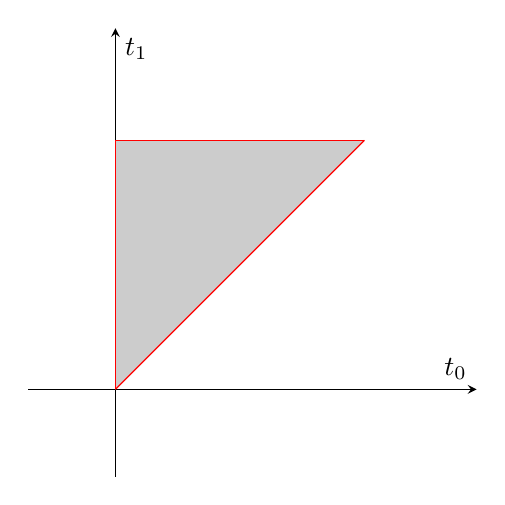
\begin{tikzpicture}
      \begin{axis}[
      axis equal image,
      axis lines = middle,
      enlargelimits,
      xtick=\empty,
      ytick=\empty,
      xlabel = {$t_0$},
      ylabel = {$t_1$},
        xmin = -0.2, xmax = 1.3,
        ymin = -0.2, ymax = 1.3,
      ]
      \fill[black!20] (axis cs:0,0) -- (axis cs:1,1) -- (axis cs:0,1) -- cycle;
      \addplot[domain=0:1, samples=2, red] ({x}, {1});
      \addplot[domain=0:1, samples=2, red] ({x}, {x});
      \addplot[domain=0:1, samples=2, red] ({0}, {x});
    \end{axis}
  \end{tikzpicture}
\end{center}


  我们固然可以将其看作一个带状区域,而我们有两种积分方式
  \[Vol(V_2(x)) = \int_{V_2(x)} 1 \, dx dy = \int_{0}^{x}\, dt_0 \int_{t_0}^{x}\, dt_1 = \int_{0}^{x} \, dt_1 \int_{0}^{t_1}\, dt_0\]

  \[
    \begin{aligned}
      &\quad\int_{V_2(x)} f(t_0)\, dt \\
      &= \int_{0}^{x}\, dt_0 \int_{t_0}^{x}\, dt_1 f(t_0) = \int_{0}^{x} dt_0 f(t_0) \int_{t_0}^x dt_1\\
      &= \int_{0}^{x}dt_1 \int_{0}^{x}dt_0 f(t_0)\\
    \end{aligned}  
    \]
    
  我们重新考虑一般的情形
  \[\begin{aligned}
    &\quad\int_{V_m(x)} f(t_0)\, dt\\
    &= \int_{0}^{x}dt_0 \int_{t_0}^{x}dt_1\cdots \int_{t_{m - 2}}^{x} dt_{m - 1}f(t_0) = \int_{0}^{x}\, dt_0 f(x_0) \int_{t_0}^{x}dt_1\cdots \int_{t_{m - 2}}^{x} dt_{m - 1} = \int_{0}^{x}\, dt_0 f(x_0) \frac{(x - t_0)^{m - 1}}{(m - 1)!}\\
    &= \int_{0}^{x}dt_{m - 1}\int_{0}^{t_{m - 1}}dt_{m - 2}\cdots \int_{0}^{t_1}dt_0 f(t_0)\\
  \end{aligned}\]

  注意到上下两种积分方式的求解难度完全不同,第一种方式要简单很多.
\end{example}

我们重新考虑我们的体积定义
\begin{definition}
  特征函数\\

  \[\chi_D = \begin{cases}
    1 , x\in D\\
    0 , x \notin D\\
  \end{cases}\]
\end{definition}

\begin{definition}
  Jordan测度\\

  \[Vol(D) = \int_{Q \supset D} \chi_D dx\]
\end{definition}

我们这里没有限定这是一个什么区域,我们尝试使用上和下和的方式来考察它

注意到我们的边界处的小方块,我们的标志点如果选在边界外,那么就是$0$,如果在边界内,就是$1$,我们接下来考察
\[U(\chi_D,P) - L(\chi_D,P) = \sum_{\partial D \cap Q_J \neq \varnothing} \omega_J Vol(Q_J) = \sum_{\partial D \cap Q_J \neq \varnothing} Vol(Q_J)\]

如果说这个区域的体积是存在的,那么就要求边界部分的体积为$0$.

\begin{definition}
  零测度集\\

  $Q \subset \RR^m$是一个闭方块,对于集合$\Lambda \subset Q$,若$\forall \varepsilon > 0$,$\exists Q$的分割$P$,使得
  \[\sum_{\Lambda \cap Q_J \neq \varnothing} Vol(Q_J) < \varepsilon\]
  则称$\Lambda$是零测集
\end{definition}

上述定义中的\textbf{维度}非常重要,我们可以使用一个例子说明

\begin{example}
  对于一条线段,在$\RR^1$中考虑,其测度显然不为$0$,但如果我们在$\RR^2$中考察它,那么正如我们前面考虑带状区域的引理中的证明,覆盖其集合的方块体积可以任意小,因此其测度为$0$
\end{example}

$Q \subset \RR^2$,$Q$中\textbf{有限长}线是零测集

闭方块内还能做无限长的线吗?我们接下来会讲到这一点.

\begin{theorem}
  若$f(x)$的不连续点是零测集(几乎处处连续) $\Rightarrow f(x) \in R(D)$
\end{theorem}

\begin{cproof}
  这里的证明过程本质上还是把小方块分成两部分,连续的部分其振幅可以小于任意数[一致连续],不连续的部分体积可以小于任何值[零测集的定义],因此二者加起来振幅和也可以小于任意小的值.具体证明过程省略.
\end{cproof}

\begin{definition}
  Jordan可测集\\

  对一个集合$D \subset Q \subset \RR^m$,若其边界$\partial D$是零测集,则称$D$是Jordan可测集[相当于是说我们在这个区域特征函数是可积的].
\end{definition}

\begin{definition}
  任意区域上的积分\\


  \[\tilde{f}(x) = f(x) \chi_D(x) = \begin{cases}
    f(x)\, x \in D\\
    0, x \notin D\\
\end{cases}\]

于是我们定义$D$上的积分为
\[\int_{D} f(x)\, dx \equiv \int_{Q} \tilde{f}(x)\, dx\]
\end{definition}

以下是一些常见的性质(相同)\\

\begin{theorem}
  在Jordan可测集上的函数具有线性性质[这里没有指明积分域是因为其对其他情形同样成立]
  \[\int \alpha f + \beta g = \alpha \int f + \beta \int g\]
\end{theorem}

\begin{theorem}
  单调性
\end{theorem}

\begin{theorem}
  中值定理\\
\end{theorem}

\begin{theorem}
  对于互不相交的集合$D_i$,$D_i \cap D_j = \varphi(i \neq j)$,则
  \[\int_{\cup_i D_i} f = \cup_i \int_{D_i} f\]
\end{theorem}

下面我们来回答前面为什么要规定$Q \subset \RR^2$,$Q$中\textbf{有限长}的线是零测集

\begin{example}
  
  Hilbert space-filling curve:
  
我们四等分方块,将四个方块的中心连成$n$形

继续四等分方块,利用这个方块内已有的半段继续作$n$形,然后再将四个方块内的线首尾相连,以此类推.

我们发现每一次递归,线的总长度可以变为原来的$2$倍以上,也就是说我们可以无限的做下去,得到无限长的曲线.

这样的曲线不是零测集,因为我们本质上递归过程是在做分割,而我们的分割使得每个小方块内都有曲线上的点,因此我们必须选取所有小方块才能覆盖这条线,其Jordan测度为$1$.这让我们思考Jordan测度是否有不完美的地方.
\end{example}

\subsection{重积分的变量代换}
对于一些复杂区域上的积分,我们可以考虑做变量代换,使得$x,y$空间中的不规则小区域$D_{J'}$可以由$u,v$空间中的规则闭方块映射而来

\[\sigma(f,\xi,P) = \sum_{J} \tilde{f}(J) Vol(Q_J) = \sum_{J'} f(\xi_{J'}) Vol(D_{J'})\]

当我们在$u,v$空间中时
\[\sum_{J'} f(\xi_J') Vol(D_J') = \sum_{J'} f(\varphi^{-1}(\xi_J)) Vol(D_J')\]

我们首先考虑一元的情形
$\varphi,f: \RR \to \RR \to \RR$,于是就有
\[\int_{\varphi(u_0)}^{\varphi(u_1)}f(x)\, dx = \int_{u_0}^{u_1} f(\varphi(u)) \varphi'(u)\, du\]

之后考虑二元的情形

$u-v$坐标系下的一个小方块$(u_0,v_0),(u_0,v_0 + \Delta v),(u_0 + \Delta u,v_0),(u_0 + \Delta u, v_0 + \Delta v)$将会由$\varphi$映射到$(x_0,y_0),(x_1,y_1),(x_2,y_2),(x_3,y_3)$,且有
\[(x_0,y_0) = \varphi(u_0,v_0),(x_1,y_1) = \varphi(u_0 + \Delta u,v_0),(x_2,y_2) = \varphi(u_0,v_0 + \Delta v),(x_3,y_3) = \varphi(u_0 + \Delta u,v_0 + \Delta v)\]

因为这里我们的$\Delta u,\Delta v$很小,我们可以将$(x_0,y_0),(x_1,y_1),(x_2,y_2),(x_3,y_3)$视作一个平行四边形,于是我们在局部可以将映射近似为一个线性映射

于是我们可以考虑泰勒展开
\[x_1 = x(u_0,v_0) + \Delta u~ x_u(u_0,v_0) + O(\Delta u^2)\]
\[y_1 = y(u_0,v_0) + \Delta u~ y_u(u_0,v_0) + O(\Delta u^2)\]
\[x_2 = x(u_0,v_0) + \Delta v~ x_v(u_0,v_0) + O(\Delta v^2)\]
\[y_2 = y(u_0,v_0) + \Delta v~ y_v(u_0,v_0) + O(\Delta v^2)\]

这样我么唯一确定了一个平行四边形,可以定义
\[\ve{a} = (x_1,y_1) - (x_0,y_0) = (x_u \Delta u,y_u \Delta u) + O(\Delta u^2), \ve{b} = (x_2,y_2) - (x_0,y_0) = (x_v \Delta v,y_v \Delta v) + O(\Delta v^2)\]

这个平行四边形的面积也就是
\[
\begin{aligned}
Vol(D) = \|\ve{a} \times \ve{b}\| &= |(x_u y_v - x_v y_u)| \Delta u \Delta v + O(\Delta u^2 \Delta v, \Delta v^2 \Delta u)\\
&= \det \left|\begin{pmatrix}
  x_u&x_v\\
  y_u&y_v\\
\end{pmatrix}\right| \Delta u \Delta v + O(\Delta u^2 \Delta v, \Delta v^2 \Delta u) \\
\end{aligned}  \]

也就是说我们近似的有
\[\Delta x \Delta y = \left|\frac{\partial (x,y)}{\partial(u,v)}\right| \Delta u \Delta v\]

我们前面对这个小区域做了一个估计,接下来我们要度验证这样的估计是可行的

我们假设对每个方向做$N$等分,注意我们的高阶量量阶为$\frac{1}{N^3}$,从而整体的体积量阶为$\frac{1}{N^2}$,因此可以认为其是可以忽略的.

\begin{theorem}
  对于映射$\varphi = (\varphi_1,\varphi_2) \in C^1(\Omega)$,其中$\Omega$是一个开集,$\varphi : \Omega \subset \RR^2 \to \RR^2$,且$E \subset \Omega$ Jordan可测,若
  \begin{enumerate}
    \item $\frac{\partial(\varphi_1,\varphi_2)}{\partial(u,v)} \neq 0,\forall (u,v) \in int(E)$
    \item $\varphi$是单的
  \end{enumerate}
  则$\varphi(E)$是若当可测的.若取$\forall f\in C(\varphi(E))$,则可做变量替换
  \[\int_{\varphi(E)} f(x)\, dx = \int_{E} f(\varphi(u)) \left|\frac{\partial \varphi}{\partial u}\right|\, du\]
\end{theorem}

这里证明的难点是
\[\varphi(\partial E) \neq \partial(\varphi(E))\]

这个难点我们可以使用以下的例子展示

\begin{example}
  对于区域
  \[\begin{cases}
    v \geq 0\\
    u^2 + v^2 = 1\\
  \end{cases}\]

  \begin{center}
  
    \begin{tikzpicture}
      \begin{axis}[
      axis equal image,
      axis lines = middle,
      enlargelimits,
      xtick=\empty,
      ytick=\empty,
      xlabel = {$u$},
      ylabel = {$v$},
      % legend pos = north east,
      % legend cell align = {left},
      % legend style = {draw=none}
    ]
      \addplot[domain=0:180, samples=60, red] ({cos(x)}, {sin(x)});
      \addplot[domain=-1:1, samples=2, red] (x,0);
      % \addplot[domain=-1:1, samples=2, cyan] (x,-1);
      % \addplot[domain=-1:1, samples=2, cyan] (1,x);
      % \addplot[domain=-1:1, samples=2, cyan] (-1,x);
    \end{axis}
  \end{tikzpicture}
  
  \end{center}
  我们做变量代换
  \[\begin{cases}
    x = u^2 - v^2\\
    y = 2uv\\
  \end{cases}\]

  那么原先的圆弧边界
  \[\begin{cases}
    u = r \cos \theta\\
    v = r \sin \theta\\
  \end{cases}\]

  就变成圆
  \[\begin{cases}
    x = r^2 \cos 2\theta\\
    y = r^2 \sin 2\theta\\
  \end{cases}\]
  \begin{center}
  
    \begin{tikzpicture}
      \begin{axis}[
      axis equal image,
      axis lines = middle,
      enlargelimits,
      xtick=\empty,
      ytick=\empty,
      xlabel = {$x$},
      ylabel = {$y$},
      % legend pos = north east,
      % legend cell align = {left},
      % legend style = {draw=none}
    ]
      \addplot[domain=0:360, samples=60, red] ({cos(x)}, {sin(x)});
      \addplot[domain=0:1, samples=2, red] (x,0);
      % \addplot[domain=-1:1, samples=2, cyan] (x,-1);
      % \addplot[domain=-1:1, samples=2, cyan] (1,x);
      % \addplot[domain=-1:1, samples=2, cyan] (-1,x);
    \end{axis}
  \end{tikzpicture}
  
  \end{center}

  原先的底边就不再是边界了
\end{example}

在什么情况下我们做变量代换呢?

当我们的积分区域是由若干个函数的等值线例如$u(x,y) = \alpha,u(x,y) = \beta, v(x,y) = \gamma,v(x,y) = \delta$所包围的区域时

\begin{example}
  对于曲线$y = qx,y = px(0 < p < q)$和曲线$xy = a,xy = b(0 < a < b)$围成的面积,我们即求积分
  \[\int_{D} ~1 d(x,y)\]

  我们做变量替换$u = xy,v = \frac{y}{x}$,从而有
  \[\frac{\partial(u,v)}{\partial(x,y)} = \det \begin{pmatrix}
    y & x\\
    -\frac{y}{x^2}&\frac{1}{x}\\
  \end{pmatrix} 2\frac{y}{x} = 2v\]

  注意我们需要的雅可比行列式其实是
  \[\frac{\partial(x,y)}{\partial(u,v)} = \frac{1}{\frac{\partial(u,v)}{\partial(x,y)}} = \frac{1}{2v}\]

  于是转化为
  \[V = \int_{[a,b]\times[p,q]} 1 \abs{\frac{1}{2v}}\, d(u,v) = \frac{1}{2 }(b - a) \ln\parameter{\frac{q}{p}}\]
\end{example}

\begin{example}
  极坐标变换

  $x = r\cos \theta,y = r \sin \theta$,于是
  \[\frac{\partial(x,y)}{\partial(r,\theta)} = \abs{\det\begin{pmatrix}
    \cos\theta & - r \sin \theta\\
    \sin \theta & r \cos \theta\\
  \end{pmatrix}} = r\]

  于是对于一个小弧元
  \[Vol = r \Delta r \Delta\theta\]
\end{example}

\begin{example}
  \[\begin{aligned}
    I = \int_{-\infty}^{+\infty} e^{-x^2}\, dx\\
  \end{aligned}\]

  我们这里可以利用放缩
  \[e^{-x^2} \leq \frac{1}{1 + x^2}\]

  先证明这个积分收敛,然后,我们记
  \[I(a) = \int_{-a}^{a} e^{-x^2}\, dx\]
  \[\begin{aligned}
    I^2(a) &= \int_{-a}^{a} e^{-x^2}\, dx\int_{-a}^{a} e^{-y^2}\, dy\\
    &= \int_{[-a,a]\times[-a,a]} e^{-x^2 - y^2} d(x,y)\\
  \end{aligned}\]

  我们可以将这个正方形区域的积分放缩为内切圆内和外接圆内的积分
  \[\int_{x^2 + y^2 \leq a^2} e^{-x^2 - y^2} \leq I^2(a) \leq  \int_{x^2 + y^2 \leq 2a^2} e^{-x^2 - y^2}\]

  于是就通过极坐标换元,左侧化为
  \[\int_{[0,a] \times [0,2\pi]} e^{-r^2} r\, d(r,\theta) = \int_{0}^{2\pi} d\theta \int_{0}^{a} e^{-r^2} r \, dr = \pi (1 - e^{-a^2})\]

  右侧化为
  \[\pi (1 - e^{-2a^2})\]

  于是取$a \to +\infty$的极限利用夹逼原理即可得到
  \[I(a) = \sqrt{\pi}\]
\end{example}

\begin{example}
  球坐标变换
  \[\begin{cases}
    x = r \cos \varphi \cos \theta\\
    y = r \cos \varphi \sin \theta\\
    z = r \sin \varphi\\
  \end{cases}\]

  注意这几个变量的范围
  \[\begin{cases}
    0 \leq r < +\infty\\
    -\frac{\pi}{2} \leq \varphi \leq \frac{\pi}{2}\\
    0 \leq \theta \leq 2\pi\\
  \end{cases}\]
  可以化简得到其雅可比行列式为
  \[\frac{\partial(x,y,z)}{\partial(r,\theta,\varphi)} = r^2 \cos \varphi\]
\end{example}

\begin{example}
  记$D$为$x^2 + y^2 + z^2 = a^2$与$z = \sqrt{x^2 + y^2}$围成的区域(这其实时是一个圆锥状的区域),我们做球坐标变换得到
  \[I = \int_{D} (x^2 + y^2 + z^2) \, d(x,y,z) = \int_{[0,a]\times [0,2\pi]\times [\frac{\pi}{4},\frac{\pi}{2}]} r^2 r^2 \cos \varphi d(r,\theta,\varphi)\]
\end{example}

\begin{example}
  我们推广这个例子,我们对于一个$n$维空间的球,我们涉及到$n - 1$个方位角,我们可以理解为
  \[x_1^2 + x_2^2 + \cdots + x_n^2 \leq r\]

  \[x_1^2 + x_2^2 + \cdots + x_{n - 1}^2 \leq r^2 - x_n^2 = (r \cos \theta_{n - 1}^2)\]

  我们成功将其降维成一个更低维的``球坐标''.

  例如我们考虑一个$4$维空间的球坐标$(x_1,x_2,x_3,x_4) \to (r,\theta_1,\theta_2,\theta_3)$,于是可以有
  \[\begin{cases}
    x_1 = r \sin \theta_3 \sin \theta_2 \cos \theta_1\\
    x_2 = r \sin \theta_3 \sin \theta_2 \sin \theta_1\\
    x_3 = r \sin \theta_3 \cos \theta_2\\
    x_4 = r \cos \theta_3\\
  \end{cases}\]

  我们可以尝试写出一个递推式
  \[
  \begin{aligned}
  \frac{\partial(x_1,x_2,x_3,x_4)}{\partial (r,\theta_1,\theta_2,\theta_3)} &= \left|\begin{matrix}
    \frac{\partial x_1}{\partial r}&\frac{\partial x_1}{\partial \theta_1}&\frac{\partial x_1}{\partial \theta_2}&\frac{\partial x_1}{\partial \theta_3}\\
    \frac{\partial x_2}{\partial r}&\frac{\partial x_2}{\partial \theta_1}&\frac{\partial x_2}{\partial \theta_2}&\frac{\partial x_2}{\partial \theta_3}\\
    \frac{\partial x_3}{\partial r}&\frac{\partial x_3}{\partial \theta_1}&\frac{\partial x_3}{\partial \theta_2}&\frac{\partial x_3}{\partial \theta_3}\\
    \frac{\partial x_4}{\partial r}&0&0&\frac{\partial x_4}{\partial \theta_3}\\
  \end{matrix} \right|\\
    &= -\cos \theta_3~ \frac{r \cos \theta_3}{\sin \theta_3} M_{3,3} - r\sin \theta_3 M_{3,3}\\
    &=  - r ~\frac{1}{\sin \theta_3} \sin^3 \theta_3^3 J_3\\
\end{aligned}
  \]

  注意到这个行列式中第一列和最后一列的前三个分量是共线的
  \[J_4 = - r \frac{1}{\sin\theta_3} \sin^3 \theta_3 J_3 = -  r \sin^2 \theta_3 J_3\]

  同理可得
  \[J_n = -r \sin^{n - 2} \theta_{n - 1} J_{n - 1}\]
\end{example}

\section{曲线积分}
\subsection{第一型曲线积分}
如果我们的积分区域的维度比空间维度小,那么我们如何处理这样的积分呢?

例如我们考虑$\RR^m$空间中的一个$n$维曲面$D$$(n < m)$,我们如果将这个曲面用闭方块包围,那么很显然在大多数情况下,我们的曲面的``体积''是$0$,因而无法达到我们的目的,因此我们考虑做变量代换,将其转化为一个低维空间中的区域$D'$,从而
\[\dim (D) = \dim (D') = n\]

在这样的新空间中我们使用闭方块将其包围,然后同理做分割即可.\\

我们以$\RR^3$的情形为例说明:

如果我们考虑空间中的一条线,我们可以考虑将其参数化后积分,本质上是一个一维的积分,只是我们是在三维空间中考虑它

\begin{definition}
对于$r: r(t), t\in [\alpha,\beta], \RR \to \RR^3$,我们称自身没有交点或者最多只有头尾一个交点的曲线[严格表述为:$\forall t_1,t_2 \in (\alpha,\beta)$, $t_1 \neq t_2, r(t_1) \neq r(t_2)$]为简单曲线.
\end{definition}

\begin{definition}
  如果还有$r(\alpha) = r(\beta)$,我们将其称为闭合曲线(若当曲线).\\
\end{definition}

我们对曲线$\gamma$做分割$\pi = \{t_1 = \alpha < t_2 < \cdots < t_N = \beta\}$,我们对于其中的每一小段,我们都可以定义割线[相当于对曲线做了一个二阶近似]

定义$\lambda = \sum_{i = 1}^{N} \|r(t_{i - 1})  - r(t_i)|$,这样的分割很像一个Dabourx\textbf{下和},因为我们的割线总是小于我们的实际长度,而且随着我们不断细分(添加分割点),我们的总长度不断递增以曲线长度为上确界.

于是我们定义
\[l(\gamma) = \sup_{\pi} \lambda(\gamma,\pi)\]

同样我们需要证明上确界与黎曼和$\lim_{|\pi|\to 0} \lambda(\gamma,\pi)$是否同时满足(也就是说$\pi \to 0$与$\lambda(\gamma,\pi)$趋近上确界是否一定同时发生?)

\begin{theorem}
  若$\gamma$是一个简单连续曲线,则
  \[\exists \sup_\pi \lambda(\gamma,\pi) \Leftrightarrow \lim_{|\pi| \to 0} \lambda(\gamma,\pi)\]
\end{theorem}

\begin{cproof}
  $\Leftarrow$,$\forall \varepsilon > 0, \exists \delta, \forall \pi', |\pi' | < \delta$,都有
  \[|\lambda(\gamma,\pi') - I| < \varepsilon\]

  我们任取一个$\pi$,对其做加细得到分割$\tilde{\pi}$使得$|\tilde{\pi}| < \delta$

  根据范数的三角不等式,我们有
  \[\lambda(\gamma,\pi) \leq \lambda(\gamma,\tilde{\pi}) < I + \varepsilon\]

  $\Rightarrow$,记$J$为$\sup_\pi \lambda(\gamma,\pi)$的上确界,从而有$\forall \varepsilon > 0 ,\exists \pi$使得
  \[J - \varepsilon < \lambda(\gamma,\pi) < J\]

  对于任取的$\varepsilon$,我们不妨取$\pi_0$作为满足上面条件的分割.同时由于$r$是闭区间上一致连续的函数,于是$\exists \delta,\forall t_1,t_2$,如果$|t_1  - t_2| < \delta$,就有
  \[\|r(t_1) - r(t_2)\| < \frac{\varepsilon}{N_0}\]
  其中$N_0$为$\pi_0$的分割数

  对于$\forall \pi$,$|\pi| < \delta$,我们定义$\pi_1 = \pi \cup \pi_0$,于是就有
  \[J - \varepsilon < \lambda(\gamma,\pi_0) \leq \lambda(\gamma,\pi_1) \leq J\]

  同时由于$\pi_1$是$\pi$的加细,因此我们可以将$\pi$的分割点形成的区间分为以下两类,一类是包含$\pi_0$分割点的区间,一类是不包含$\pi_0$分割点的区间
  \[\lambda(\gamma,\pi) = \sum_{\text{不含}\pi_0\text{分割点}} \|r(t_i) - r(t_{i - 1})\| + \sum_{\text{含有}\pi_0\text{分割点}} \|r(t_i) - r(t_{i - 1})\|\]
  \[\lambda(\gamma,\pi_1) = \sum_{\text{不含}\pi_0\text{分割点}} \|r(t_i) - r(t_{i - 1})\| + \sum_{\text{含有}\pi_0\text{分割点}} \|r(t_{i - 1}) - r(\tau_i)\| + \|r(\tau_i) - r(t_i)\|\]

  \[\lambda(\gamma,\pi_1) - \lambda(\gamma,\pi) < \sum_{\text{含有}\pi_0\text{分割点}} \|r(t_{i - 1}) - r(\tau_i)\| + \|r(\tau) - r(t_i)\| < 2\frac{\varepsilon}{N_0} N_0 = 2 \varepsilon\]

  从而有任意一个这样的分割$\pi,|\pi| < \delta$,就有
  \[J \geq \lambda(\gamma,\pi) > \lambda(\gamma,\pi_1) - 2\varepsilon > J - 3\varepsilon\]

  于是就有
  \[\lim_{|\pi| \to 0} \lambda(\gamma,\pi) = J\]
\end{cproof}

如果进一步增强条件,$r \in C^1[\alpha,\beta]$, $l(\gamma) = \int_{\alpha}^{\beta} \|r'(t)\|dt$,这里$\|r'(t)\|dt$也可以表示为前面所讲的$ds$


\begin{definition}
  第一型曲线积分\\

  对于一个可求长曲线$\gamma: r(t), t \in [\alpha,\beta]$,对于分割$\pi$,我们定义
  \[\Delta S_i = \|r(t_{i - 1}) - r(t_i)\|\]

  对于函数$f(x)$,我们定义曲线积分
  \[\int_{\gamma} f(r(s))\, ds \equiv \lim_{|\pi| \to 0} \sum_{i} f(Q_i) \Delta S_i\]

  其中标志点$Q_i \in \{r(t), t \in [t_{i - 1},t_i]\}$

  若$r(t) \in C^1$,那么还有
  \[\int_{\gamma} f(r(s))\, ds = \int_{\alpha}^{\beta}f(\gamma(t))\|r'(t)\| dt\]
\end{definition}

\begin{example}
  我们有一个形如弹簧的曲线[螺线]$r = (a\cos t,a \sin t,b t)$,我们定义曲线的密度$\rho = \rho + \rho_1 \sin t, t \in [0,T]$.

  我们首先可以对曲线做一阶导
  \[r' = (-a \sin t, a \cos t, b)\]
  
  从而
  \[\|r'(t)\| = \sqrt{a^2 + b^2}\]
  
  我们积分的质量也就是
  \[\int_{0}^{T}(\rho_0 + \rho_1 \sin t) \sqrt{a^2 + b^2}\, dt = \sqrt{a^2 + b^2}(\rho_0 T + \rho_1(\cos T - 1))\]
\end{example}

\subsection{第一型曲面积分}
接下来我们考虑曲面的积分,对于$S: r(\ve{u}), \ve{u} = (u,v)$.

我们定义
\begin{definition}
  \begin{itemize}
    \item 简单曲面$r(\ve{u})$:$r(\ve{u}) \in C$,且为单射
    \item 正则曲面
    \begin{equation}
      r(\ve{u}) :r \in C^1, r_u \times r_v \neq 0
    \label{regularcurve}
    \end{equation}[$r_u , r_v$不平行,这样才能``张成''一个面元]
    \end{itemize}
\end{definition}

在前面的曲线积分中,我们可以采用割线来近似我们的曲线,但在这里,我们的一个小面元,我们是否可以做一个内接的小平面来近似我们曲面的面积?我们这里采用了一个切平面来近似

我们考察一个小面元$r(u,v),r(u + \Delta u, v),r(u,v + \Delta v)$,考虑$r_u \Delta u,r_v \Delta v$这两个向量,它们张成的平行四边形面积和原本曲面的面积有什么关系?

\[\sigma(S_J) = \|r_u \times r_v\| \Delta u \Delta v\]

我们可以验证这两个面积的差是一个高阶小量$\Delta u^2 \Delta v + \Delta v^2 \Delta u$,于是我们就可以考虑黎曼和

\[\sigma(S) = \lim_{|\pi| \to 0} \sum_{J} \sigma(S_J)\]

前面我们的正则条件保证了小面元不是$0$.

我们先来考虑$r_u \times r_v$
\[r_u \times r_v = \abs{\begin{matrix}
  i & j & k\\
  x_u & y_u & z_u\\
  x_v & y_v & z_v\\
\end{matrix}} = \begin{pmatrix}
  \frac{\partial(y,z)}{\partial(u,v)} & \frac{\partial(z,x)}{\partial(u,v)} & \frac{\partial(x,y)}{\partial(u,v)}
\end{pmatrix}\]

这样的三个分量分别对应了我们的曲面在三个坐标平面上的投影面积,于是
\[\|r_u \times r_v\| = \sqrt{\parameter{\frac{\partial(y,z)}{\partial(u,v)}}^2 + \parameter{\frac{\partial(z,x)}{\partial(u,v)}}^2 + \parameter{\frac{\partial(x,y)}{\partial(u,v)}}^2}\]

利用叉乘的另外一种定义也就有
\[\|r_u \times r_v\| = \|r_u\| \|r_v\| |\sin \theta| \]

这样的小面元和我们的曲面第一基本形式有什么关联吗?

回顾曲面的第一基本形式
\[r_u \cdot r_v = \|r_u\| \| r_v\| \cos \theta\]

于是我们这里的叉乘也就可以转化为
\[\|r_u \times r_v\| = \sqrt{\|r_u\|^2 \|r_v\|^2 - (r_u \cdot r_v)^2} = \sqrt{E G - F^2}\]

\begin{definition}
  第一型曲面积分\\

  \[\int_{S} f(x) d\sigma = \int_{D} f(x(u)) \|r_u \times r_v\| d(u,v)\]

  其中$D$是我们$u,v$的定义域,注意$d\sigma$只是一种形式的记号,并不能简单写为$dxdy$这种东西
\end{definition}

在曲线的情形,我们让
\[\sup_\pi \lambda(\gamma,\pi) = \lim_{|\pi| \to 0} \lambda(\gamma,\pi)\]

那么这在曲面的情形下还成立吗?也就是说不同分割下曲面最大的面积与分割趋近于$0$时曲面的面积是否相等?

\begin{example}
  我们考虑一个半圆柱面,首先等式右边是存在的(极限显然就是我们曲面的面积),假设我们采用内接三角形来近似,那么我们也可以来考虑细分,每一个三角形的面积我们都可以投影到底面上,从而放缩可得
  \[\lambda_2 > 4 R^2 ,\cdots, \lambda_n > 2n R^2\]

  也就是说等式的左边的上确界不存在

  本质上是因右边的极限同时限制了两个分量,然而左侧的极限可能在一个分量取极限,另一个分量正常的情况下发散[上面就是这样]\\
\end{example}

\begin{example}
  我们考虑三维空间中的二维曲面$f(x,y) \in C^1$,$z = f(x,y)$,$(x,y) \in D$,于是有
  \[r(x,y) = \begin{cases}
    x = x\\
    y = y\\
    z = f(x,y)\\
  \end{cases}\]
  \[\begin{cases}
    r_x = (1,0,f_x)\\
    r_y = (0,1,f_y)\\
    r_u \times r_v = (f_x,-f_y,1)
  \end{cases}\]
  
  于是我们的曲面积分就转化为了平面上的积分
  \[\int_S 1 ~ d\sigma = \int_{D} \sqrt{f_x^2 + f_y^2 + 1} \, dx dy\]
\end{example}

\begin{example}
  球面面积\\
  
  对于一个半径为$a$的球,我们考虑使用球坐标来表达
  \[r = (a \cos \varphi\cos \theta,a\cos \varphi \sin \theta,a \sin \varphi), \theta \in [0,2\pi], \varphi \in \bracket{-\frac{\pi}{2},\frac{\pi}{2}}\]
  \[\begin{cases}
    r_\theta = (-a \cos\varphi \sin \theta,a \cos \varphi\cos \theta,0)\\
    r_\varphi = (-a\sin \varphi \cos \theta,-a \sin \varphi\sin \theta,a \cos \varphi)\\
    r_\theta \times r_\varphi = (a^2 \cos^2 \varphi\cos \theta,a^2 \cos^2\varphi \sin \theta,a^2 \sin \varphi,\cos\varphi)\\
  \end{cases}\]

  \[\|r_\theta \times r_\varphi\| = a^2 \cos \varphi\]

  于是球面积
  \[A = \int_{0}^{2\pi} d\theta \int_{-\frac{\pi}{2}}^{\frac{\pi}{2}} d\varphi a^2 \cos\varphi = 4 \pi a^2\]
\end{example}

\begin{example}
  螺旋面面积\\

  对于螺旋面$S : r = (a\cos t,a\sin t,bt)$,$t \in [0,T], a \in [0,R]$,我们计算$S$上函数$z$的积分.

  我们已知的有
  \[\begin{cases}
    r_t = (-a \sin t,a\cos t,b)\\
    r_a = (\cos t, \sin t,0)\\
    r_t \times r_a = (-b \sin t,b\cos t,a)\\
  \end{cases}\]
  于是
  \[\|r_t\times r_a \| = \sqrt{a^2 + b^2}\]

  积分
  \[\int_{S} z d\sigma = \int_{0}^{T}dt \int_{0}^{R} d t \sqrt{a^2 + b^2} da =bT \int_{0}^{R} \sqrt{a^2 + b^2} da\]
\end{example}

\subsection{第二型曲线积分}
第二型曲线积分的实际物理场景是变力做功
\begin{definition}
  
对于曲线$\Gamma: r(t): \RR \to \RR^3,t \in [t_0,t^\ast]$,且$r(t) \in C[t_0,t^\ast]$.我们在空间中存在向量场$F(x)$.

对于$[t_0,t^\ast]$,我们可以做分割,其中的任意一段如$[t_{i - 1},t_i]$,对应于曲线上的分割从$x_{i - 1} = r(t_{i - 1})$到$x_i = r(t_i)$,只要我们的分割够短,我们就可以用曲线的切线/割线作近似.

对于我们的标志点
\[Q_i \in \{r(t), t \in [t_{i - 1},t_i]\}\]

我们每一个小分割上的做功
\[F(Q_i) \cdot (x_i - x_{i - 1}) = F(Q_i) \cdot \Delta x_i\]

于是它们的总和就是
\[\sum_{i = 1}^{N} F(Q_i) \cdot \Delta x_i\]

我们可以设向量场为$F = (F^{(x)},F^{(y)},F^{(z)})$,取极限
\[\lim_{\|\Delta x\|\to 0} \sum_{i = 1}^{N} F(Q_i) \cdot \Delta x_i = \lim_{\|\Delta x\| \to 0} \sum_{i = 1}^{N}(F^{(x)} dx + F^{(y)}dy + F^{(z)} dz)\]

我们记
\[\int_\Gamma F\cdot dx \equiv \lim_{\|\Delta x\|\to 0} \sum_{i = 1}^{N} F(Q_i) \cdot \Delta x_i = \int_\Gamma \parameter{F\cdot \frac{dx}{ds}} ds = \int_{t_0}^{t^\ast} F\cdot \frac{dx}{dt}dt\]

注意这里的$\Gamma$不仅要给出曲线,还需要给出曲线的方向.
\end{definition}

其中$\int_\Gamma \parameter{F\cdot \frac{dx}{ds}} ds$也就是我们的被积函数的形式,我们把方向有关的信息都给了被积函数.\\

由于我们的第二型曲线积分本质上和黎曼积分没有什么区别,因此我们可以得到关于其的许多性质

\begin{theorem}
  线性
  \[\int_\Gamma (\alpha F + \beta G) dx = \alpha\int_\Gamma F dx + \beta \int_\Gamma Gdx\]
\end{theorem}

\begin{theorem}
  可加性
  \[\int_{\Gamma_1 + \Gamma_2}  = \int_{\Gamma_1} + \int_{\Gamma_2}\]

  其中$\Gamma_1,\Gamma_2$是两条曲线,且前后相接.

  同时我们定义
  \[\int_{\Gamma} = - \int_{-\Gamma}\]
\end{theorem}

\begin{example}
  我们考虑重力场$g$下沿曲线$\Gamma$从$(x_1,y_1,z_1)$到$(x_2,y_2,z_2)$的做功.

  \[W = \int_\Gamma (0,0,-mg)\cdot dx = \int_{z_A}^{z_B} -mg dz = -mg(z_B - z_A)\]
\end{example}

\begin{example}
  对于椭圆$\Gamma: \frac{x^2}{a^2} + \frac{y^2}{b^2} = 1$,我们定义向量场$F = \frac{1}{2}(x,-y)$

  \[\oint_\Gamma F \cdot dx = \frac{1}{2}\oint_\Gamma ydx - xdy\]

  我们可以考虑将$\Gamma$参数化为
  \[\begin{cases}
    x = a\cos \theta\\
    y = b\sin \theta\\
  \end{cases}\]

  于是就被转化为
  \[\frac{1}{2}\oint_\Gamma ydx - xdy = \frac{1}{2} \int_0^{2\pi} (b \sin \theta a \sin \theta + a \cos \theta b \cos \theta)\, d\theta = \pi ab\]

  这恰好等于椭圆的面积,这是一个巧合吗?之后我们会在``不同积分之间的关系''中讨论.事实上,对于任意的闭合区域,都有这样的``巧合''.
\end{example}

\begin{example}
  螺旋线
  \[\Gamma :\begin{cases}
    x = a\cos \theta\\
    y = a\sin \theta\\
    z = b\theta\\
  \end{cases},\theta \in [0,T]\]

  事实上当我们将曲线参数化时我们就定义了这个曲线的方向,这个方向为
  \[\frac{\frac{dx}{d\theta}}{\left\|\frac{dx}{d\theta}\right\|}\]

  我们考虑向量场$F = (x,y,z)$,此时的曲线积分为
  \[\int_\Gamma F\cdot dx = \int_\Gamma d \parameter{\frac{1}{2} \|x\|^2} = \parameter{\frac{1}{2}\|x\|^2}\bigg|_{\theta = 0}^{\theta = T} =  \frac{1}{2}\parameter{a^2 + b^2 \theta^2}\bigg|_{\theta = 0}^{\theta = T} = \frac{1}{2}b^2 T^2\]

  这与我们的$a$是无关的,因为无论$a$如何改变,向量场方向与螺线在$x-y$平面的投影方向都是垂直的,最总和贡献为$0$
\end{example}

\subsection{第二型曲面积分}
我们考虑实际问题中的流量问题,我们有
\[Q = \lim_{|P| \to 0} \sum_{J} v_J \cdot n_J \Delta \sigma_J = \int_S v \cdot dS = \int_S (v \cdot n) d\sigma \]

这相当于变成了一个第一型曲面积分.

$dS = n d\sigma$是一个有向面积(类比在Frenet标架中,我们有$dx = T ds$).

我们对曲面做一个参数化表示$S: r(u,v)$,$r(u,v) \in C^1$我们知道
\[n = \frac{r_u \times r_v}{\|r_u \times r_v\|}\]

为什么需要连续可微?因为例如正方体的表面,在其顶点和棱处,显然没办法找出法向来.\\

但是,我们仍然需要更加严格的定义方向

例如,我们可以将一个条带粘成环,这样的环是可以定向的,法向可以区分环的内外.然而,我们同样也可以将其粘成莫比乌斯带,虽然我们在每个局部都可以定义方向,但是从整体来看方向必然会产生冲突,我们怎样来参数表达它们的区别呢?

对于这个``筒'',我们可以定义
\[x = (a\cos u, a \sin u, v), a = const, u \in [0,2\pi], v \in [-b,b]\]

问题:$n|_{u = (0,0)}$与$n|_{u = (2\pi,0)}$是否相等?

我们只要考虑两点的法向就行
\[\begin{cases}
  r_u = (-a\sin u,a\cos u, 0)\\
  r_v = (0,0,1)\\
  r_u \times r_v = (a\cos u,a \sin u)\\
\end{cases}\]

因此
\[(r_u \times r_v)|_{u = (0,0)} = (a,0,0),(r_u \times r_v)|_{u = (2\pi,0)} = (a,0,0)\]

然而对于莫比乌斯带
\[r = ((a + v\sin \frac{u}{2})\cos u,(a + v\sin \frac{u}{2})\sin u, v\cos \frac{u}{2})\]

\[r_u = (-(a + v\sin \frac{u}{2})\sin u + \frac{v}{2}\cos \frac{u}{2}\cos u, (a + v\sin \frac{u}{2})\cos u + \frac{v}{2}\sin \frac{v}{2} \cos u,- \frac{v}{2}\sin \frac{v}{2})\]
\[r_v = (\sin \frac{u}{2}\cos u, \sin \frac{u}{2} \sin u, \cos \frac{u}{2})\]

我们可以求出
\[u = (0,0),\begin{cases}
  r_u = (0,a,0)\\
  r_v = (0,0,1)\\
  r_u \times r_v = (a,0,0)\\
\end{cases}, u = (2\pi,0),\begin{cases}
  r_u = (0,a,0)\\
  r_v = (0,0,-1)\\
  r_u \times r_v = (-a,0,0)\\
\end{cases}\]

于是我们需要对我们的区域做一些约束

\begin{definition}
  初等区域:边界是简单分段连续曲线[分段:允许有导数不存在的点]
\end{definition}

\begin{definition}
  初等曲面:定义在初等区域上的简单正则曲面(定义见\ref{regularcurve})
\end{definition}

\begin{definition}
  拼接

  \begin{enumerate}
    \item 至多两个曲面相交于一条曲线
    \item 多于三个曲面至多交于$1$点
  \end{enumerate}
\end{definition}

\begin{definition}
  诱导定向

  曲面$E$在$\partial E$的左侧
\end{definition}

\begin{definition}
  协调定向

  两个曲面\textbf{边界}$\partial E$的\textbf{定向相反}
\end{definition}

\begin{definition}
  全局正则

  任意两个曲面协调定向
\end{definition}

如果我们对莫比乌斯带进行这样的操作,那么总会有一个边界不是协调的,于是这个曲面不是全局正则的,我们不会在这种曲面上定义方向

\begin{definition}
  对于一个可定向的正则曲面$S$,我们记$n$为曲面的法向,定义一个向量$v = (v^{(1)},v^{(2)},v^{(3)})$
  \[\int_S v \cdot n d\sigma = \int_S v \cdot dS\]
  为第二型曲面积分
\end{definition}

\begin{definition}
  对于任何一个向量,我们可以记单位法向量与三个坐标轴$x,y,z$夹角为$\alpha,\beta,\gamma$,于是这个法向量也可以写作
  \[(\cos \alpha,\cos \beta,\cos \gamma)\]
\end{definition}

那么我们的小面元乘上这些余弦值的大小是什么?其实对应于我们的小面元投影$y-z,x-z,x-y$平面上的面积.我们也不难利用
\[dS = (\cos \alpha,\cos \beta,\cos \gamma) d\sigma\]
观察到这个结果

利用微分形式中的概念,我们可以得到
\[dS = (dy \wedge dz,dz \wedge dx, dx \wedge dy)\]

我们的第二型曲面积分
\[\int_S v \cdot dS = \int_S v^{(x)} dy \wedge dz + v^{(y)} dz \wedge dx + v^{(z)} dz \wedge dy\]

这样的形式上的东西很像我们的行列式.

由于这三个项相加我们可以独立的去计算,因此我们可以考虑将这个第二型曲面积分转化为第一型曲面积分.

我们在第一型曲面积分中知道
\[d\sigma = \|r_u \times r_v\| d(u,v)\]

因此有
\[
\begin{aligned}  
  \int_S v\cdot n d\sigma &= \int_D v \frac{r_u \times r_v}{\|r_u \times r_v\|} \|r_u\times r_v\| d(u,v)\\
  &= \int_D v \cdot \left|\begin{matrix}
    i & j & k\\
    x_u & y_u & z_u\\
    x_v & y_v & z_v\\
  \end{matrix}\right|\\
  &= \int_D v^{(x)} \frac{\partial(y,z)}{\partial(u,v)}d(u,v) + v^{(y)}\frac{\partial(z,x)}{\partial(u,v)}d(u,v) + v^{(z)}\frac{\partial(x,y)}{\partial(u,v)}d(u,v)
\end{aligned}  
\]

\begin{example}
  对于我们的半径为$a$的球面,我们积分其外侧,我们考虑
  \[I = \frac{1}{3} \iint_S r \cdot dS = \frac{1}{3} \iint_S r \cdot n d\sigma = \frac{1}{3} \iint_S r \cdot \frac{r}{\|r\|} d\sigma = \frac{4}{3}\pi a^3 \]

  为什么我们做的是曲面积分却得到了一个体积?这是巧合吗?不是,我们接下来在``各类积分的关系''中讨论.
\end{example}

\subsection{各型积分的关系}
\subsubsection{格林公式}
\begin{example}
  我们再举一个例子来验证我们的猜想,对于曲面$S$
  \[S = \{(x,y,z) | |x| \leq a,|y| \leq a, |z| \leq a\}\]
  同时我们取其外侧,我们的积分依然是
  \[I = \frac{1}{3}\iint_S r\cdot dS\]

  我们可以分成$6$个面分别来积分,最终可以得到
  \[I = 6 \cdot \frac{4}{3} a^3 = 8a^3\]
\end{example}

\begin{example}
  对于任意的椭球$S : \frac{x^2}{a^2} + \frac{y^2}{b^2} + \frac{z^2}{c^2} = 1$,我们同样可以验证积分
  \[\frac{1}{3}\iint_S r \cdot dS = \frac{4}{3}\pi abc\]
\end{example}

前面的例子中反映了什么特点?一个边界的积分转化为了一个区域上的积分,这和我们的微积分基本定理(牛顿莱布尼茨公式)十分相似,后者同样是将边界[区间端点]和区域[区间]关联起来.

\begin{example}
  第二型曲线积分与面积分的关联

  做一个边界为$x = a,x = b$的$X$型区域$D$,其上下分别为$y_1(x),y_0(x)$这两条曲线.并且规定$y_0(x) < y_1(x)$,$y_0(x),y_1(x) \in C^1[a,b]$
  \[D = \{(x,y)| x \in [a,b] ,y \in [y_0(x),y_1(x)]\}\]

  我们做第二型曲线积分
  \[
  \begin{aligned}
    \int_{\partial D} P(x,y)\, dx &= \int_{\gamma_0} P(x,y)dx + \int_{\gamma_1} P(x,y)dx\\
    &= \int_{a}^b P(x,y_0(x))\, dx + \int_b^a P(x,y_1(x))\, dx\\
    &= \int_a^b \parameter{P(x,y_0(x)) - P(x,y_1(x))} dx\\
    &= \int_a^b \parameter{\int_{y_0(x)}^{y_1(x)} - \frac{\partial P(x,y)}{\partial y} dy}dx\\
    &= \int_a^b \int_{y_0(x)}^{y_1(x)} \parameter{-\frac{\partial P}{\partial y}(x,y)}d(x,y)\\
    &= \int_D \parameter{-\frac{\partial P}{\partial y}(x,y)}d(x,y)\\
  \end{aligned}  
  \]
\end{example}

我们先来考虑区域$D$更加复杂的情况,我们可以对区域$D$进行横向和纵向的分割得到多个带状区域$D_1,D_2,D_3,D_4$,这时我们就必须考虑划分得到的边界的处理.回顾我们的\textbf{协调定向}的概念,我们的边界处积分方向相反,因而它们的和为$0$,最后剩余的部分就是我们这个区域$D$的第二型曲线积分
\[\int_{\partial D} P\, dx = \int_{\cup_i \partial D_i} P \, dx = \sum_{i} \int_{\partial D_i} P\, dx = \sum_{i} \int_{D_i} \parameter{-\frac{\partial P}{\partial y}} d(x,y) = \int_D \parameter{-\frac{\partial P}{\partial y}} d(x,y)\]

注意这里的积分是第二型的,因为方向是很重要的,否则不能抵消!

前面我们讨论了$X$型区域,那么对于$Y$型区域也是如此,只是符号上有所差别:对于区域$D = \{(x,y)| y\in [c,d], x \in [x_0(y),x_1(y)]\}$

\[
  \begin{aligned}
    \int_{\partial D} Q(x,y)dy &= \int_{\gamma_0}Q(x,y)\, dy + \int_{\gamma_1}Q(x,y)\, dy\\
    &= -\int_{c}^d Q(x_0(y),y)\, dy + \int_c^d Q(x_1(y),y)\, dy\\
    &= \int_{c}^d \parameter{Q(x_1(y),y) - Q(x_0(y),y)}\, dy \\
    &= \int_c^d \int_{x_0(y)}^{x_1(y)} \parameter{\frac{\partial Q}{\partial x}(x,y)}dx dy\\
    &= \int_D \frac{\partial Q}{\partial x}d(x,y)\\
  \end{aligned}
  \]

对于更加复杂的区域,我们可以进行分割得到$X$型区域和$Y$型区域,将所有小区域的结果相加起来根据前面定向的讨论,就可以得到

\begin{theorem}
  格林公式\\

  对于$\Omega \subset \RR^2$,设其为由有限条连续曲线围成的闭区域,函数$P(x,y),Q(x,y) \in C^1(\Omega)$,则
  \[\int_{\partial \Omega} Pdx + Qdy = \int_{\Omega} \parameter{\frac{\partial Q}{\partial x} - \frac{\partial P}{\partial y}} d(x,y) = \int_{\Omega} \left|\begin{matrix}
    \partial_x & \partial_y\\
    P & Q\\
  \end{matrix}\right| d(x,y)\]

  注意这里的$\partial \Omega$需要取边界曲线的正向:若一个人沿着$\Omega$的某个方向前进时,若$\Omega$始终在其\textbf{左侧}

  关于定向,我们可考虑下面的示意图:
  \begin{center}
    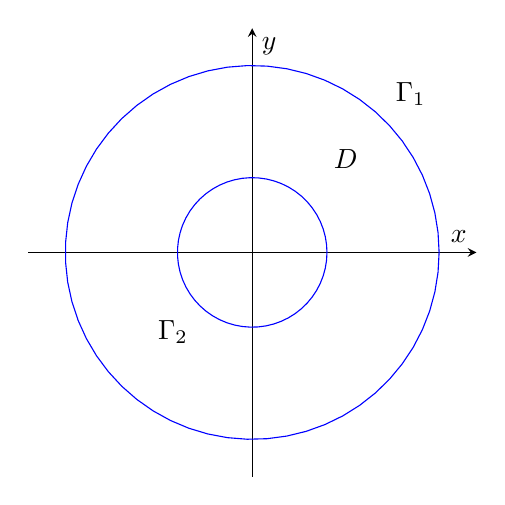
\begin{tikzpicture}
        \begin{axis}[
            axis equal image,
            axis lines = middle,
            enlargelimits,
            xtick=\empty,
            ytick=\empty,
            xlabel = {$x$},
            ylabel = {$y$},
        ]
            \addplot[domain=0:360, samples=60, blue] ({cos(x)}, {sin(x)});
            \addplot[domain=0:360, samples=60, blue] ({0.4 * cos(x)}, {0.4 * sin(x)});

            \node at (axis cs:0.5,0.5) {$D$};
            \node at (axis cs:{1.2*cos(45)},{1.2*sin(45)}) {$\Gamma_1$};
            \node at (axis cs:{0.6*cos(225)},{0.6*sin(225)}) {$\Gamma_2$};
        \end{axis}
    \end{tikzpicture}
\end{center}
这里中间的$D$是我们的积分区域,外侧的$\Gamma_1$的正向是逆时针方向,而内侧$\Gamma_2$的正向则是顺时针方向
\end{theorem}

我们怎样理解和记忆这样的公式呢?其实可以利用行列式
\[\left|\begin{matrix}
  i & j & k\\
  \partial_x & \partial y & 0\\
  x & y & 0\\
\end{matrix}\right| = (0,0,\partial_x Q - \partial_y P)\]

注意等式的两边``量纲''必须一致,因此右侧一定要有导数的项

\begin{example}
  对于积分
  \[I_C = \oint_C \frac{xdy - ydx}{x^2 + y^2}\]
  假设
  \begin{itemize}
    \item $C : x^2 + y^2 = a^2$
  \end{itemize}
  那么我们可以做变量代换
  \[\begin{cases}
    x = a\cos \theta\\
    y = a\sin \theta\\
  \end{cases},\theta\in[0,2\pi]\]

  \[I_C = \int_{0}^{2\pi} \frac{a\cos \theta a\cos \theta + a\sin \theta a\sin \theta}{a^2 \cos^2\theta + a^2 \sin^2 \theta} d\theta= 2\pi\]

  这里背后的几何意义是什么?
  \begin{center}
  
    \begin{tikzpicture}
      \begin{axis}[
      axis equal image,
      axis lines = middle,
      enlargelimits,
      xtick=\empty,
      ytick=\empty,
      xlabel = {$x$},
      ylabel = {$y$},
      % legend pos = north east,
      % legend cell align = {left},
      % legend style = {draw=none}
    ]
      \addplot[domain=0:360, samples=60, blue] ({cos(x)}, {sin(x)});
      % \addplot[domain=-1:1, samples=2, cyan] (x,1);
      % \addplot[domain=-1:1, samples=2, cyan] (x,-1);
      % \addplot[domain=-1:1, samples=2, cyan] (1,x);
      % \addplot[domain=-1:1, samples=2, cyan] (-1,x);
    \end{axis}
  \end{tikzpicture}
  
  \end{center}
  我们考虑向量$F = \parameter{\frac{x}{x^2 + y^2},\frac{-y}{x^2 + y^2}}= \frac{1}{a}(\cos \theta,\sin \theta)$,其方向是我们圆上的切线,而我们$(dx,dy)$的方向与其平行.

  \begin{itemize}
    \item 我们的曲线不包围原点时
  \end{itemize}
  我来考虑其他区域,如果我们的区域不包含原点,我们的$\theta$应该会回到原来的大小

  \begin{center}
  
    \begin{tikzpicture}
      \begin{axis}[
      axis equal image,
      axis lines = middle,
      enlargelimits,
      xtick=\empty,
      ytick=\empty,
      xlabel = {$x$},
      ylabel = {$y$},
      % legend pos = north east,
      % legend cell align = {left},
      % legend style = {draw=none}
    ]
      \addplot[domain=0:360, samples=60, blue] ({-1 + cos(x)/3}, {1 + sin(x)/3});
      % \addplot[domain=-1:1, samples=2, cyan] (x,1);
      % \addplot[domain=-1:1, samples=2, cyan] (x,-1);
      % \addplot[domain=-1:1, samples=2, cyan] (1,x);
      % \addplot[domain=-1:1, samples=2, cyan] (-1,x);
    \end{axis}
  \end{tikzpicture}
\end{center}
  当我们的区域不包含原点时,此时没有了$(0,0)$这一个瑕点[因为我们的黎曼积分要求函数有界],因此我们可以使用格林公式
  \[I_C  = \int_E \bracket{\frac{\partial}{\partial x}\parameter{\frac{x}{x^2 + y^2}} - \frac{\partial}{\partial y} \parameter{\frac{-y}{x^2 + y^2}}} d(x,y) = 0\]

  \begin{itemize}
    \item $C$包围原点时
  \end{itemize}
  当我们的区域包围$(0,0)$点时,我们可以在这个区域内作一个圆,在这个区域内挖掉一个圆.内部圆的边界为$C$,于是
  \[\int_{C + C'} F\cdot dx = \int_G = 0\]

  因此
  \[\int_C F \cdot dx = - \int_{C'} F\cdot dt = 2\pi\]

  注意这里的$C'$的定向和我们最初讨论$C$是包围原点的圆时的定向不同
\end{example}
\subsubsection{高斯公式}

在本节中,我们考虑曲面$D$围成的区域,记其$\partial D$的侧为$D$的\textbf{外侧}!这一点非常重要,意味着如果我们积分的是曲面的内侧则要\textbf{添加负号}!\\

我们考虑$\RR^3$中的一个桶状区域,我们的区域$\Omega$位于曲面$z = z_0(x,y)$与$z = z_1(x,y)$之间,其中$(x,y) \in D$.我们考虑边界上的曲面积分.\\

首先我们先考虑在$x-y$平面的投影,因此我们侧面的部分对这部分积分没有贡献,我们记顶面和底面分别为$\partial \Omega_1,\partial \Omega_0$,注意它们的定向是相反的
\[
\begin{aligned}  
  \oiint_{\partial \Omega} F(x,y,z) dx \wedge dy &= \iint_{\partial \Omega_1} F(x,y,z)dx\wedge dy +\iint_{\partial \Omega_2} F(x,y,z)dx\wedge dy\\
  &= \iint_D F(x,y,z_1(x,y)) d(x,y) - \iint_D (F(x,y,z_0(x,y)))d(x,y)\\
  &= \iint_D \parameter{\int_{z_0}^{z_1} \frac{\partial F}{\partial z}(x,y,z) dz}\, dx dy\\
  &= \iiint_{\Omega} \frac{\partial F}{\partial z}(x,y,z)d(x,y,z)\\
\end{aligned}  
\]

对于两个曲面的公共边界,它们的法向是相反的,因此它们这个面上的曲面积分可以相互抵消.\\

同理我们可以作$z-x$,$y-z$平面上的积分,
\[\iint_{\partial \Omega}G dz \wedge dx = \iiint_{\Omega} \frac{\partial G}{\partial y} d(x,y,z)\]
\[\iint_{\partial \Omega} H dy \wedge dz = \iiint_{\Omega} \frac{\partial H}{\partial z} d(x,y,z)\]
我们可以最终得到高斯公式
\begin{theorem}
  对于$F = (F^{(x)},F^{(y)},F^{(z)}) \in C^1(\Omega)$,则有
  \[\oiint_{\partial \Omega} F\cdot dS = \iiint_{\Omega} \nabla \cdot F dx\]
\end{theorem}

\begin{example}
  我们回顾一下之前的一个例子
  \[\frac{1}{3} \oiint_{\partial \Omega} (x,y,z) \cdot dS = \frac{1}{3} \iiint_{\Omega} 3 d(x,y,z) = Vol(\Omega)\]
\end{example}

我们继续考虑如何参数化,我们假设边界可以描述为$r(u,v)$,于是
\[\frac{1}{3} \oiint_{\partial \Omega} (x,y,z)\cdot dS = \frac{1}{3} \iint_{u \in D} (x,y,z) \cdot (r_u\times r_v)d(u,v) = \frac{1}{3} \iint_D\left|\begin{matrix}
  x & y & z\\
  x_u & y_u & z_u\\
  x_v & y_v & z_v\\
\end{matrix}\right|\]

这里面的系数其实是一个与维度相关的系数,这个行列式代表的体积其实是一个斜着的圆筒的体积,我们想要的其实是一个从原点出发的斜圆锥的体积,因此我们这里会有系数$\frac{1}{3}$.
\subsubsection{斯托克斯公式}
我们前面考虑了一个$\RR^2$中的曲面[区域]与其边界之间的关系,如果我们考虑$\RR^3$中的二维曲面及其边界,我们应该也能有类似的结论.

我们考虑这个曲面边界上的第二型曲线积分,我们假设这个曲面是正则的,也就是说我们可以将其参数化映到$u-v$空间中的一个区域.

\[
\begin{aligned}  
  \oint_{\partial E}P(x,y,z) dx &= \oint_{\partial D} P(x(u,v),0,0) \parameter{\frac{\partial x}{\partial u} du + \frac{\partial x}{\partial v} dv}\\ 
  &= \oint_{\partial D} Px_u du + P x_v dv\\
  &= \iint_D \parameter{\partial_u(P x_v) - \partial_v(P x_u)}d(u,v)\\
  &= \iint_D \parameter{P_u x_v - P_v x_u}d(u,v)\\
  &= \iint_D \bracket{(x_u \cdot \nabla P) x_v - (x_v \cdot \nabla P)x_u} d(u,v)\\
  &= \iint_D \bracket{(x_u P_x + y_x P_y + z_y P_z)x_v - (x_v P_x + y_v P_y + z_v P_z)x_u} d(u,v)\\
  &= \iint_D \bracket{(y_u x_v - y_v x_u)P_y + (z_u x_v - z_v x_u)P_z} d(u,v)\\
  &= \iint_D - P_y \frac{\partial(x,y)}{\partial(u,v)}d(u,v) + P_z \frac{\partial(z,x)}{\partial(u,v)}d(u,v)\\
  &= \iint_E -P_y dx\wedge dy + P_z dz\wedge dx\\
\end{aligned}  
\]

注意前面符号的记忆方式:我们这里讨论的是$x$的情况,那么当形如$dx\wedge dy$这种$y$在后的项时,取负号,而形如$dz\wedge dx$这种$z$在前的项时,取正号\\

前面我们只考虑了$x$的情况,我们类似可以得到
\[\oint_{\partial E} Q dy = \int_E -Q_z dy \wedge dz + Q_x dx\wedge dy \]
\[\oint_{\partial E} R dz = \int_E -R_x dz \wedge dx + R_y dy\wedge dz \]

在斯托克斯公式中,我们需要我们的变量是$C^2$的,这究竟是否必要的[我们在这里的证明中利用了$x_{uv} = x_{vu}$]
\begin{theorem}
  斯托克斯公式
  \[\oint_{\partial E} v \cdot dx = \int_E \nabla \times v \cdot dS\]

  其中
  \[\nabla \times v = \left|\begin{matrix}
    i & j & k\\
    \partial_x & \partial_y & \partial_z\\
    v^{(x)} & v^{(y)} & v^{(z)}\\
  \end{matrix}\right|\]

  我们可以对照我们前面的各分量结果验证我们这里的结论.

  注意这里边界的定向规则如下:我们由法向$n$确定$E$的一侧,当一个人\textbf{站立与}$n$\textbf{一致}时沿某个方向前进时,曲线围成的区域$E$始终在其\textbf{左侧},则称这个方向为边界的正向[不难理解其实我们在$\RR^2$上的格林公式其实是默认取法向为$n = (0,0,1)$]
\end{theorem}

注意在三维空间中任意一条若当曲线可以产生无穷多种曲面,这里的结果意味着我们不管取什么样的曲面都有曲面积分相同,我们任取$E_1,E_2$这两个曲面,合并它们得到一个闭合曲面,那么我们能否使用高斯公式将其继续转化?
\[
  \begin{aligned}  
    \int_{\partial E} \cdot dx - \int_{\partial E} v\cdot dx &= \iint_{E_1} \nabla \times v \cdot dS - \iint_{E_2} \nabla \times v \cdot dS\\
    &= \iint_{\partial \Omega} \nabla \times v\cdot dS\\
    &= \iiint_{\Omega} \nabla \cdot(\nabla \times v )d(x,y,z)\\
  \end{aligned}
  \]
这意味着
\[\nabla \cdot (\nabla \times v) = 0\]

这是应当成立的,因为行列式的两项已经相等了

\subsection{微分形式简介}
我们这里想要得到的结论是
\[\int_{\partial \Omega} \omega = \int_{\Omega}d\omega\]

这将说明我们的牛顿莱布尼茨公式,斯托克斯公式,高斯公式本质上是一样的.

\begin{definition}
  在$\RR^n$空间中,我们定义$p$次微分形式($p-$形式)
  \[\omega = \sum_{i_1,i_2,\ldots,i_p} a_{i_1,i_2,\ldots,i_p} dx^{i_1}\wedge dx^{i_2}\wedge \times \wedge dx^{i_p}, i_1,i_2,\ldots,i_p\in \{1,2,\ldots,n\},a_{i_1,i_2,\ldots,i_p} \in \RR\]
\end{definition}

\begin{example}
  举例一些常见的形式
  \begin{itemize}
    \item $f(x)$为$0$形式
    \item $v\cdot dv$为$1$形式
    \item $F\cdot dS$为$2$形式
  \end{itemize}
\end{example}

\begin{definition}
  (1)线性
  \[\alpha \sum_{i} a_i dx^{i_1}\wedge \cdots \wedge dx^{i_p} + \beta \sum_{i} b_i dx^{i_1}\wedge \cdots \wedge dx^{i_p} = \sum_i (\alpha a_i+ \beta b_i) dx^{i_1}\wedge \cdots \wedge dx^{i_p}\]

  (2)外积(楔积)$\wedge$,满足如下性质
  \begin{enumerate}
    \item $dx^{i} \wedge dx^{i} = 0$
    \item $dx^{i} \wedge dx^{j} = -dx^{j} \wedge dx^{i}$
  \end{enumerate}
\end{definition}

\begin{example}
  对于$0-$形式$f$和$p-$形式$\omega$,有
  \[f\wedge \omega = f\omega = \omega \wedge f\]

  对于$p-$形式$\omega$,$q-$形式$\mu$,
  \[\omega = \sum_{i} a_i dx^{i_1}\wedge \cdots \wedge dx^{i_p} , \mu = \sum_i b_j dx^{j_1}\wedge \cdots \wedge dx^{j_q} \]

  则得到一个$p + q-$形式
  \[\omega\wedge \mu = \sum_{i,j} = a_i b_j dx^{i_1}\wedge \cdots \wedge dx^{i_p}\wedge dx^{j_1}\wedge \cdots \wedge dx^{j_q}\]
\end{example}

我们的外积具有如下性质:
\begin{theorem}
  线性:
  \[(f_1\omega_1 + f_2 \omega_2) \wedge \mu = f_1\omega_1  \wedge \mu + f_2 \omega_2 \wedge \mu\]

  反交换律:
  \[\omega \wedge \mu = (-1)^{pq}\mu \wedge \omega\]

  结合律
  \[(\omega \wedge \mu)\wedge \gamma = \omega \wedge (\mu \wedge \gamma)\]
\end{theorem}
我们不难有,在$\RR^m$空间中,任意$n > m$,都有$n-$形式为$0$

我们的$1-$形式只有$n$个,我们假设
\[\omega^i = \sum_{j = 1}^{n} a_j^i dx^{j}\]
于是我们就有
\[\omega^1 \wedge \omega^2 \wedge \cdots \wedge \omega^n = \det(a_j^i) dx^1 \wedge dx^2 \wedge\cdots \wedge dx^n\]

这里需要一定的证明,但是我们可以直观的感受到反对称性以及其他性质与行列式的相似性.

我们知道
\[\omega^i = \sum_{j = 1}^{n} \frac{\partial f^i}{\partial x^j} dx^j\]

于是
\[\omega^1 \wedge \omega^2 \wedge \cdots \wedge \omega^n = \frac{\partial(f^1,\ldots,f^n)}{\partial(x_1,\ldots,x_n)} dx^1 \wedge dx^2 \wedge\cdots \wedge dx^n\]

我们考虑$d$这个算子,若$f$是一个$0-$形式,那么
\[df = \sum_{i} \frac{\partial f}{\partial x^i} d x^i\]

若$\omega$是一个$p-$形式,则
\[d\omega = \sum d a_{i_1 i_2\cdots i_p} \wedge dx^{i_1}\wedge \cdots\wedge dx^{i_p}\]

相当于我们的$d$是一个从$p-$形式到$(p + 1)-$形式的算子

不难发现其满足以下性质
\begin{theorem}
  \begin{enumerate}
    \item $d(\omega_1 + \omega_2) = d\omega_1 + d\omega_2$
    \item 对于$p-$形式$\omega$,$q-$形式$\mu$,有$d(\omega \wedge \mu) = d\omega \wedge \mu + (-1)^p \omega \wedge d \mu$
    \item $dd \omega = 0$
  \end{enumerate}
\end{theorem}

\begin{cproof}
  (3)
  \[d\omega = \sum_{i,r} \frac{\partial a_i}{\partial x^r} dx^r \wedge (dx^{i_1} \wedge \cdots \wedge dx^{i_p})\]
  \[
  \begin{aligned}
    dd \omega &= \sum_{i,r,s} \frac{\partial^2 a_i}{\partial x^r \partial x^s} dx^s \wedge dx^r \wedge (dx^{i_1} \wedge \cdots \wedge dx^{i_p})\\
    &= \sum_{i,r,s} \frac{\partial^2 a_i}{\partial x^s \partial x^r} dx^r \wedge dx^s \wedge (dx^{i_1} \wedge \cdots \wedge dx^{i_p})\\
    &= - \sum_{i,r,s} \frac{\partial^2 a_i}{\partial x^r \partial x^s} dx^r \wedge dx^s \wedge (dx^{i_1} \wedge \cdots \wedge dx^{i_p})\\
    &= 0
    \end{aligned}
  \]
\end{cproof}


我们接下来讨论以下
\[\begin{aligned}
  d(v\cdot dx) &= d(v^{(x)} dx + v^{(y)} dy + v^{(z)} dz)\\
  &= (v^{(x)}_x dx + v^{(x)}_y dy + v^{(x)}_z dz) \wedge dx\\
  &+ (v^{(y)}_x dx + v^{(y)}_y dy + v^{(y)}_z dz) \wedge dy\\
  &+ (v^{(z)}_x dx + v^{(z)}_y dy + v^{(z)}_z dz)\wedge dz\\
  &= (v_y^{(z)} - v_z^{(y)}) dy\wedge dz + (v_z^{(x)} - v_x^{(z)}) dz \wedge dx + (v_x^{(y)} - v_y^{(x)}) dx \wedge dy\\
\end{aligned}\]

也就是有
\[\oint_{\partial D} v\cdot dx = \int_D d(v\cdot dx)\]

同理我们也可以利用外微分来证明我们的高斯公式
\[\iint_{\partial \Omega} v\cdot dS \int_\Omega d(v\cdot dS)\]

推广到一般的情况也就是
\[\int_{\partial \Omega} \omega = \int_\Omega d\omega\]

\subsection{场论入门}

\begin{definition}
  定义哈密尔顿算符$\nabla = (\partial_x, \partial_y,\partial_z)$
\end{definition}
\subsubsection{数量场的梯度}
\begin{definition}
对于一个数量值函数$f$,其梯度为$\nabla f$,记作$\text{grad}~ f$.

\end{definition}
如果$e$是等值线$f = C$的切向量,则有
\[e \cdot \nabla f = 0\]

\subsubsection{向量场的散度}
\begin{definition}
  对于一个向量值函数$v$,其散度定义为$\nabla \cdot v$,记作$\text{div}~ v$.

  我们不妨考虑高斯公式中
  \[\oiint_{\partial \Omega} v \cdot dS = \iiint_{\Omega} \nabla \cdot v d\ve{x}\]

  我们就可以考虑
  \[\lim_{L \to 0} \frac{1}{Vol(\Omega)} \iiint_{\Omega} \nabla \cdot v dx = \nabla \cdot v(x_0)\]
\end{definition}

\subsubsection{向量场的旋度}
\begin{definition}
  对于一个向量值函数$v$,其旋度定义为$\nabla \times v$,记作$curl v$

  我们不妨考虑一个环路中的斯托克斯公式
  \[ \oint_{\partial D} v\cdot d\ve{x} = \iint_D \nabla \times v \cdot dS\]

  于是可以定义旋度为
  \[\lim_{L \to 0}\frac{1}{Area(D)} \iint_{D} \nabla \times v\cdot dS\]
\end{definition}

\subsubsection{部分场论公式的证明}

\begin{theorem}
  \[\nabla \cdot (F \times G) = - F \cdot (\nabla \times G) + (\nabla \times F) \cdot G\]
\end{theorem}
\begin{cproof}
  \[\begin{aligned}
    \nabla \cdot (F \times G) &= \sum_{l,m,n} \partial_l(F_m G_n) e_l \cdot (e_m \times e_n)\\
    &= \sum_{l,m,n}  (\partial_l F_m) G_n \varepsilon_{lmn} + (\partial_l G_n) F_m\varepsilon_{lmn}\\
    &= (\nabla \times F) \cdot G - (\nabla \times G) \cdot F\\
  \end{aligned}\]

  其中利用了
  \[(\nabla \times F)_n=\varepsilon_{lmn}\partial_{l}F_{m}, (\nabla \times G)_m =\varepsilon_{lnm} \partial_{l}G_{n}= -\varepsilon_{lmn}\partial_{l}G_{n}.\]
\end{cproof}  

\begin{theorem}
  \[\nabla \times (F \times G) = (F \cdot \nabla) G - (G \cdot \nabla) F + (\nabla \cdot G) F - (\nabla \cdot F)G\]
\end{theorem}

\begin{cproof}
  \[\begin{aligned}
    \nabla \times (F \times G) &= \sum_{l,m,n}\partial_l (F_m G_n) e_l \times (e_m \times e_n)\\
    &= \sum_{l,m,n} \partial_l (F_m G_n) (\delta_{ln} e_m - \delta_{lm} e_n)\\
    &= \sum_{l,m}\partial_l(F_m G_l) e_m - \sum_{l,m}\partial_l(F_l G_m) e_m\\
    &= \sum_{l,m} \partial_l(F_m G_l - F_l G_m)e_m\\
    &= \sum_{l,m}(\partial_l F_m e_m)G_l + (\partial_l G_l)F_m e_m - (\partial_l F_l) G_m e_m - (\partial_l G_m e_m)F_l\\
    &= \sum_{l,m} (\partial_l F_m e_m)G_l - (\partial_l G_m e_m) F_l + (\partial_l G_l)F_m e_m - (\partial_l F_l)G_m e_m\\
    &= \sum_{l} (\partial_l F)G_l - (\partial_l G)F_l + (\partial_l G_l) F - (\partial_l F_l)G\\
    &= (G\cdot \nabla) F - (F\cdot \nabla)G + (\nabla \cdot G) F -(\nabla \cdot F)G\\
  \end{aligned}\]

  % 其中最后的转化为
  % \[\sum_l (\partial_l F)G_l = \sum_{l}\begin{pmatrix}
  %   F^1_l\\
  %   F^2_l\\
  %   F^3_l\\
  % \end{pmatrix}G_l\]
\end{cproof}


% 利用爱因斯坦求和标记,我们可以有
% \[\nabla \times v = \varepsilon_{ijk} \partial_j v_k e_i\]

% 从而有
% \[
% \begin{aligned}
%   \nabla \times (\mu \times v) &= \varepsilon_{mni} \partial_n(\varepsilon_{ijk} u_j v_k) e_m\\
%   &= \varepsilon_{imn} \varepsilon_{ijk} \partial_n(u_j v_k) e_m\\
%   &= (\delta_{mj}\delta_{nk} - \delta_{mk} \delta_{nj})\partial_n(u_j v_k) e_m\\
%   &= \partial_k (u_j u_k) e_j - \partial_j (u_j v_k)e_k\\
%   &= (\partial_k u_j) u_k e_j + u_j \partial_k u_k e_j - (\partial_j u_j)v_k e_k - u_j \partial_j v_k e_k\\
%   &= v \cdot \nabla u + (\nabla \cdot v) u - (\nabla \cdot u) v - u\cdot \nabla v\\
% \end{aligned}
% \]

% 其中
% \[\varepsilon_{ijk} = \begin{cases}
%   1, i,j,k\text{为}1,2,3\text{的轮换}\\
%   -1, i,j,k\text{为}2,1,3\text{的轮换}\\
%   0, otherwise\\
% \end{cases}\]


\begin{example}
  数值函数的梯度场: 有势无旋的矢量场

  首先考虑梯度场的散度
  \[\nabla \cdot (\nabla f) = \partial_{xx} f + \partial_{yy} f + \partial_{zz} f\]

  外力有势的含义是$\exists \varPhi$使得
  \[F = \nabla \varPhi\]

  再考虑梯度场的旋度
  \[\nabla \times \nabla f = 0\]

  这可以利用行列式来理解
  \[\left|\begin{matrix}
    i & j & k\\
    \partial_x & \partial_y & \partial_z\\
    \partial_x f& \partial_y f& \partial z f\\
  \end{matrix}\right|\]

  这告诉我们一个有势的力的做功与路径无关.

  \[\int_{\Gamma_1} F\cdot dx - \int_{\Gamma_2} F \cdot dx = \oint_{\Gamma} F \cdot dx = \iint_D \nabla \times F \cdot dS = \iint_D \nabla \times \nabla \varPhi \cdot dS = 0\]
\end{example}

\begin{example}
  旋度场的散度与旋度
  \[\nabla \cdot (\nabla \times v) = \begin{pmatrix}
    \partial_x & \partial_y & \partial_z\\
  \end{pmatrix}\begin{pmatrix}
    i & j & k\\
    \partial_x & \partial_y & \partial_z\\
    P & Q & R\\    
  \end{pmatrix} =  \begin{pmatrix}
    \partial_x & \partial_y & \partial_z\\
    \partial_x & \partial_y & \partial_z\\
    P & Q & R\\    
  \end{pmatrix} = 0\]

  这是因为相当于我们做了两次外微分,第一次相当于是斯托克斯公式,第二次相当于是高斯公式,将$\omega$转换为了$d^2 \omega$.最后结果显然为$0$

  \[
  \begin{aligned}  
  \nabla \times (\nabla \times v) &= \sum_{l,m,n} \partial_{l} \partial_{m} v_n e_l \times (e_m \times e_n)\\
  &= \sum_{l,m,n} \partial_{l} \partial_{m} v_n(\delta_{ln} e_m - \delta_{lm} e_n)\\
  &= \sum_{l,m} \partial_{l}\partial_{m} v_m e_m - \sum_{l,m} \partial_{l} \partial_{l} v_m e_m\\
  &= \nabla (\nabla \cdot v) - \sum_{l} \partial^2_l v\\
  &= \nabla (\nabla \cdot v) - \Delta v\\
  \end{aligned}
  \]

\end{example}
\subsubsection{正交曲线坐标系}
空间中的点也可以使用曲线坐标$(q_1,q_2,q_3)$来表示
\[\begin{cases}
  q_1 = q_1(x,y,z)\\
  q_2 = q_2(x,y,z)\\
  q_3 = q_3(x,y,z)\\
\end{cases}\]

于是我们原先的坐标又可以表示为
\[\begin{cases}
  x = x(q_1,q_2,q_3)\\
  y = y(q_1,q_2,q_3)\\
  z = z(q_1,q_2,q_3)\\
\end{cases}\]

如果有$\frac{\partial r}{\partial q_1},\frac{\partial r}{\partial q_2},\frac{\partial r}{q_3}$彼此正交,那么我们称上述由$q_1,q_2,q_3$确定的坐标系为\textbf{正交曲线坐标系}.

定义$\hat{e}_1,\hat{e}_2,\hat{e}_3$为空间任意一点$M$点的曲线坐标$q_1,q_2,q_3$在该点的切线单位矢量,并且指向我们$q_1,q_2,q_3$增大的方向.

% 在某一条坐标线$q_i$上,其余的坐标是给定的,于是
% \[\begin{cases}
%   x = x(q_i)\\
%   y = y(q_i)\\
%   z = z(q_i)\\
% \end{cases} \Rightarrow r = r(q_i)\]

% 从而就利用曲线各分量导数与切向量的关系得到
我们将这些切向量单位化得到
\[\frac{\partial r}{\partial q_i} = h_i \hat{e}_i\]

其中我们的$h_i$称为拉维系数.不难发现我们对偏导得到的向量取模即可得到拉维系数的值\\

需要注意的是,这里的$\hat{e}_i,h_i$等都是随着位置的变化而变化的,类似于Frenet标架.\\

\paragraph{梯度在正交曲线坐标系下得表示\\}
我们先来考虑数值函数的梯度在新的基下的表示[注:以下过程中默认采用爱因斯坦求和约定]

首先我们得梯度本身可以表示为
\[\nabla f = \frac{\partial f}{\partial x_i}e_i \]
之后我们考虑将$e_i$在我们新的一组基上作正交投影,也就是
\[
\begin{aligned}  
\nabla f &= \frac{\partial f}{\partial x_i} (e_i \cdot \hat{e}_j) \hat{e}_j\\
&= \frac{\partial f}{\partial q_k} \frac{\partial q_k}{\partial x_i} (e_i \cdot \hat{e}_j) \hat{e}_j\\
&= \frac{\partial f}{\partial q_k} \parameter{\nabla q_k\cdot \hat{e}_j} \hat{e}_j\\
\end{aligned}
\]

注意到我们的新的坐标系是正交的,也就是说
\[\frac{\partial q_k}{\partial q_l} = \delta_{kl} = \frac{\partial q_k}{\partial x_i} \frac{\partial x_i}{\partial q^l} = \nabla q_k \cdot h_l \hat{e}_l\]

不难有
\[\nabla q_k = \frac{1}{h_k} \hat{e}_k\]

于是代回就有
\[\nabla f = \frac{\partial f}{\partial q_k} \frac{1}{h_k}(\hat{e}_k \cdot \hat{e}_j) \hat{e}_j = \frac{1}{h_j} \frac{\partial f}{\partial q_j} \hat{e}_j\]


\begin{example}
  对于$x = r\cos \theta,y = r\sin\theta$,于是我们有
  \[h_r = \left\|\frac{\partial \ve{r}}{\partial r}\right\| = \sqrt{\cos^2\theta + \sin^2\theta} = 1\]
  \[h_\theta = \left\|\frac{\partial \ve{r}}{\partial \theta}\right\| = \sqrt{r^2\cos^2\theta + r^2 \sin^2 \theta} = r\]

  于是我们代入前面的式子
  \[\nabla f = \frac{\partial f}{\partial r} \hat{e}_r + \frac{1}{r}\frac{\partial f}{\partial \theta} \hat{e}_\theta\]
\end{example}

我们再从微分形式的角度来考虑$f$的梯度
\[
\begin{aligned}
  dr = dx_i e_i &= dq^j \frac{\partial x_i}{\partial q^j} e_i\\
  &= dq^j \frac{\partial r}{\partial q^j}\\
  &= dq^j h_j \hat{e}_j\\
  \end{aligned}
\]
\[
\begin{aligned}  
df &= dr \cdot \nabla f = dq \cdot \nabla f = dq^j \frac{\partial f}{\partial q^j}\\
&= dq^j h_j \hat{e}_j \cdot \nabla f\\
\end{aligned}
\]

再次利用我们$\hat{e}_j$的正交性,我们可以得到
\[\nabla f = \frac{1}{h_j} \frac{\partial f}{\partial q^j}\hat{e}_j\]

\paragraph{散度在正交曲线坐标系下的表示\\}
我们同样尝试在新的坐标下表示我们向量值函数的散度:
% 我们考虑向量值函数$v$,其在原始坐标系下可以表示为
% \[v^{(x)}dy \wedge dz + v^{(y)}dz \wedge dx + v^{(z)} dx \wedge dy\]

% 为了进一步的证明方便,我们先证明一个引理
% \begin{lemma}
%   \[\begin{aligned}
%     \nabla \cdot \parameter{\frac{\hat{e}_1}{h_2 h_3}} &= \nabla \cdot \parameter{\frac{\hat{e}_2}{h_2} \times \frac{\hat{e}_3}{h_3}}\\
%     &= \nabla \cdot (\nabla q_2 \times \nabla q_3)\\
%     &= (\nabla \times (\nabla q_2))\cdot \nabla q_3 - \nabla q_2 \cdot (\nabla \times (\nabla q_3))\\
%     &= 0\\
%   \end{aligned}\]
% \end{lemma}

假设这个向量函数在原坐标系下可以表示为
\[v = (v^{(x)},v^{(y)},v^{(z)})\]

在新的坐标系下的坐标可以表示为
\[v = (v^{(1)},v^{(2)},v^{(3)})\]

% 于是
% \[\nabla \cdot v = \nabla \cdot \parameter{v^{(1)} h_2 h_3 \frac{\hat{e}_1}{h_2 h_3} + v^{(2)} h_3 h_1 \frac{\hat{e}_2}{h_3 h_1} + v^{(3)} h_1 h_2 \frac{\hat{e}_3}{h_1 h_2}}\]

% \[\frac{\partial v^{(1)}}{\partial q_1} = \frac{\partial v^{(1)}}{\partial x^j} \frac{\partial x^j}{\partial q_1y}\]
% \[\nabla \cdot v = \frac{\partial v^{(i)}}{\partial x_i} = \frac{\partial v^{(i)}}{\partial p^j} \frac{\partial p^j}{\partial x^i}\]

我们再从微分形式的角度考虑散度:

首先如果在原坐标系下表示,则有
\[\omega = v^{(x)} dy \wedge dz + v^{(y)} dz \wedge dx + v^{(z)}dx \wedge dy\]

注意这里的$dy \wedge dz$其实已经隐含了方向的信息为$x$方向,而之后转换坐标系后的$dq_2 \wedge dq_3$隐含了方向的信息为$\hat{e}_1$方向.此时如果我们转换坐标系到正交曲线坐标系下,则有

\[
\begin{aligned}
  \omega &= v^{(1)} \frac{\partial(y,z)}{\partial (q_2,q_3)} dq_2 \wedge dq_3 + v^{(2)} \frac{\partial (z,x)}{\partial (q_3,q_1)}dq_3 \wedge dq_1 + v^{(3)} \frac{\partial (x,y)}{\partial(q_1,q_2)}dq_1 \wedge dq_2\\
  &= v^{(1)} h_2 h_3 dq_2 \wedge dq_3 + v^{(2)} h_3 h_1 dq_3 \wedge dq_1 + v^{(3)} h_1 h_2 dq_1 \wedge dq_2\\
\end{aligned}
\]

注意我们计算雅可比行列式是在新的变量下计算的,其中在新的基下有
\[\begin{pmatrix}
  \partial_{q_1} x & \partial_{q_2} x & \partial_{q_3} x\\ 
  \partial_{q_1} y & \partial_{q_2} y & \partial_{q_3} y\\ 
  \partial_{q_1} z & \partial_{q_2} z & \partial_{q_3} z\\ 
\end{pmatrix} = \begin{pmatrix}
  h_1 & 0 & 0\\
  0 & h_2 & 0\\
  0 & 0 & h_3\\
\end{pmatrix}\]

\[
\begin{aligned}
  d\omega &= \bracket{\partial_{q_1}(v^{(1)} h_2 h_3) + \partial_{q_2}(v^{(2)} h_3 h_1) + \partial_{q_3}(v^{(3)} h_1 h_2)} dq_1 \wedge dq_2 \wedge dq_3\\
  &= \bracket{\partial_{q_1}(v^{(1)} h_2 h_3) + \partial_{q_2}(v^{(2)} h_3 h_1) + \partial_{q_3}(v^{(3)} h_1 h_2)} \frac{1}{h_1 h_2 h_3} dx \wedge dy \wedge dz\\
\end{aligned}
\]

注意我们最后从$dq_1 \wedge dq_2 \wedge dq_3$代换到$dx \wedge dy \wedge dz$只是一种大小上的修正(应该认为这里的$dx,dy$和前面出现的基的转换中的不同),并不意味着我们的基变回了原先的$e_1,e_2,e_3$,不难注意到我们其他的量都是我们的$\hat{e}_1,\hat{e}_2,\hat{e}_3$下表示的!

\paragraph{旋度在正交曲线坐标系下的表示\\}
接下来我们考虑旋度:

在原始的基下,我们的微分形式可以表示为
\[\omega = v^{(x)} dx + v^{(y)} dy + v^{(z)}dz\]

之后进行变量代换就得到

\[\omega = v^{(1)}h_1 dq_1 + v^{(2)} h_2 dq_2 + v^{(3)} h_3 dq_3\]
\[
\begin{aligned}
  d\omega &= (\partial_{q_1} v^{(1)} dq_1 + \partial_{q_2} v^{(1)}dq_2 + \partial_{q_3} v^{(1)} dq_3 ) \wedge h_1 dq_1\\
  &+(\partial_{q_1} v^{(2)} dq_1 + \partial_{q_2} v^{(2)}dq_2 + \partial_{q_3} v^{(2)} dq_3 ) \wedge h_2 dq_2\\
  &+(\partial_{q_1} v^{(3)} dq_1 + \partial_{q_2} v^{(3)}dq_2 + \partial_{q_3} v^{(3)} dq_3 ) \wedge h_3 dq_3\\
  &=  (\partial_{q_2} h_3 v^{(3)} - \partial_{q_3} h_2 v^{(2)}) dq_2\wedge dq_3 + (\partial_{q_3} h_1 v^{(1)} - \partial_{q_1} h_3 v^{(3)}) dq_3 \wedge dq_1 + (\partial_{q_1} h_2 v^{(2)} - \partial_{q_2} h_1 v^{(1)})dq_1 \wedge dq_2 \\
  &= \left|\begin{matrix}
    dq_2 \wedge dq_3 & dq_3 \wedge dq_1 & dq_1 \wedge dq_2\\
    \partial q_1 & \partial q_2 & \partial q_3\\
    h_1 v^{(1)} & h_2 v^{(2)} & h_3 v^{(3)}\\
  \end{matrix}\right| = \frac{1}{h_1 h_2 h_3}\left|\begin{matrix}
    h_1 y \wedge z & h_2  z \wedge x & h_3 x \wedge y\\
    \partial q_1 & \partial q_2 & \partial q_3\\
    h_1 v^{(1)} & h_2 v^{(2)} & h_3 v^{(3)}\\
  \end{matrix}\right|\\
\end{aligned}
\]

于是我们得到旋度
\[\nabla \times v = \frac{1}{h_1 h_2 h_3} \left|\begin{matrix}
  h_1 \hat{e}_1 & h_2 \hat{e}_2 & h_3 \hat{e}_3\\
  \partial q_1 & \partial q_2 & \partial q_3\\
  h_1 v^{(1)} & h_2 v^{(2)} & h_3 v^{(3)}\\
\end{matrix}\right|\]

同样注意我们这里从$dq_2\wedge dq_3$转换到$y \wedge z$也只是一种大小上的修正

\begin{example}
  考虑球坐标
  \[\begin{cases}
    x = r\cos \varphi \cos \theta\\
    y = r\cos \varphi \sin \theta\\
    z = r\sin \varphi\\
  \end{cases}\]
  于是就有
  \[\frac{\partial \ve{r}}{\partial r} = (\cos \varphi \cos \theta, \cos \varphi \sin \theta, \sin \varphi), h_r = \left\|\frac{\partial \ve{r}}{\partial r}\right\| = 1\]

  \[\frac{\partial \ve{r}}{\partial \theta} = (- r\cos \varphi \sin \theta, r \cos \varphi \cos \theta, 0), h_\theta = \left\|\frac{\partial \ve{r}}{\partial \theta}\right\| = r\cos \varphi\]

  \[\frac{\partial \ve{r}}{\partial \varphi} = (- r \sin \varphi \cos \theta, - r \sin \varphi \sin \theta, r \cos \varphi), h_\varphi = \left\|\frac{\partial \ve{r}}{\partial \varphi}\right\| = r\]
  % \[\begin{cases}
  %   h_r = 1\\
  %   h_\theta = r\cos \varphi\\
  %   h_\varphi = r\\
  % \end{cases}\]
  其实这里间接告诉了我们在球坐标系这个正交曲线坐标系中的三个基向量
  \[\begin{cases}
    \hat{r} = (\cos \varphi \cos \theta, \cos \varphi \sin \theta, \sin \varphi)\\
    \hat{\theta} = (-  \sin \theta, \cos \theta, 0)\\
    \hat{\varphi} = (- \sin \varphi \cos \theta, - \sin \varphi \sin \theta,\cos \varphi)\\
  \end{cases}\]

  这其实是很大的认知的改变,因为我们在笛卡尔坐标系下,三个单位向量本身是不需要基本变量表示的,而这里的基向量是三个基本变量的表达式\\

  于是我们就可以得到
  \[\nabla f = \parameter{\frac{\partial f}{\partial r},\frac{1}{r \cos \varphi} \frac{\partial f}{\partial \theta},\frac{1}{r} \frac{\partial f}{\partial \varphi}}\]
  \[\nabla \cdot v = \frac{1}{r^2 \cos \varphi} \parameter{\frac{\partial}{\partial r} (r^2 \cos \varphi v^{(1)}) + \frac{\partial}{\partial \theta} (r v^{(2)}) + \frac{\partial}{\partial \varphi} (r \cos \varphi v^{(3)})}\]
  \[\nabla \times v = \frac{1}{r^2 \cos \varphi}\left|\begin{matrix}
    \hat{e}_1 & r\cos \varphi \hat{e}_2 & r \hat{e}_3\\
    \partial_r & \partial_\theta & \partial_\varphi\\
    v^{(1)} & r \cos \varphi v^{(2)} & r v^{(3)}\\
  \end{matrix}\right|\]
\end{example}

% 思考:为什么我们在计算梯度时会在正交曲线坐标系内表示梯度,而在处理散度和旋度时却最终又将坐标系转换回我们的笛卡尔坐标系呢?
% \begin{itemize}
%   \item 梯度:在任何坐标系中,梯度都是指向函数增加最快的方向的向量。在正交曲线坐标系中,我们可以直接计算每个坐标的偏导数来得到梯度。[事实上梯度操作作用于数量场效果简单以至于我们如果把坐标系变换回去,整个形式就变回去了,等于没有操作]
%   \item 散度和旋度:散度描述的是向量场的“源”或“汇”的强度,而旋度描述的是向量场的“旋转”或“涡旋”的强度。在正交曲线坐标系中,散度和旋度的计算涉及到更复杂的微分运算,因此在计算完成后,我们通常会将结果转换回原始坐标系,以便于理解和解释。
% \end{itemize}

拉普拉斯算子
\[\Delta = \nabla \cdot \nabla\]
\end{CJK}
\end{document}
\begin{itemize} 
\end{itemize}